%!TEX TS-program = xelatex 
%!TEX encoding = UTF-8 Unicode
% 
%  my_title
%
%  Created by David Perez on march 2010.
%  Copyright (c) David Perez 2010. All rights reserved.
% 
          
  
  
  
% -*- Mode:TeX -*- 
   


%% The documentclass options along with the pagestyle can be used to generate
%% a technical report, a draft copy, or a regular thesis.  You may need to
%% re-specify the pagestyle after you \include  cover.tex.  For more 
%% information, see the first few lines of mitthesis.cls. 
  
%\documentclass[12pt,vi,twoside]{mitthesis_fork_une}
%%
%%  If you want your thesis copyright to you instead of MIT, use the
%%  ``vi'' option, as above.
%%
%\documentclass[12pt,twoside,leftblank]{mitthesis_fork_une}
%%
%% If you want blank pages before new chapters to be labelled ``This
%% Page Intentionally Left Blank'', use the ``leftblank'' option, as
%% above. 

%For the final thesis
\documentclass[12pt,vi]{mitthesis_fork_une}
\pagestyle{plain}

%for technical report
%\documentclass[12pt,vi,twoside]{mitthesis_fork_une}
%\pagestyle{plain}

%for draft
%\documentclass[11pt,singlespace,draft]{mitthesis_fork_une}
%\pagestyle{drafthead}


%%package for TODO lists, comments, annotations on pdf, with colors
%\usepackage[enable, spanish, colorinlistoftodos]{todonotes}
%%el comando de abajo hace el trabajo automaticamente identificando si es un
%%draft
%\usepackage[obeyDraft]{todonotes}
%%los posibles COLORES usados para \todo[color=green!40]{test12} son:
%%green, red, blue!20!white (para mezclar dos colores)
%%la UBICACION del comentario, en el borde o entre parrafos:
%%\todo[noline]{A note with no line ...} noline o line o inline
%%\missingfigure[figwidth=6cm]{Testing a long text string}


%\usepackage[pdfborder={0 0 0}]{hyperref}
\usepackage[disable, colorinlistoftodos, textwidth=2.8cm, shadow]{todonotes}
\usepackage{amsmath} 
\usepackage[displaymath, tightpage]{preview}
 
 
\usepackage{tabularx,colortbl}
\usepackage{multirow}
\usepackage{float}
 
\usepackage[latin1]{inputenc}
\usepackage[spanish]{babel}


\usepackage{lastpage}


\usepackage{lgrind}

%% in case I include .eps versions of all figures for those w/o pdftex
%\usepackage{ifpdf}
%\ifpdf
%\usepackage[pdftex]{graphicx}
%\else
\usepackage{graphicx} 
\usepackage{epstopdf} %esto es para convertir de epd a pdf 
%\fi


\usepackage{amsmath,amssymb,amsfonts} % easily align arrays of equations
%\usepackage[pdfborder={0 0 0}]{hyperref} % hyperlinks  
\usepackage{hyperref} % hyperlinks
\usepackage{subfig} % multi-part figures
\usepackage{pdfpages} % makes it easy to insert all those nsigmapi fits



%%%%%%%%%%%%%%%%%%%%%%%%%%%%%%%%%%%%%%%%%%%%%%%%%%%%%%%%%%%%%%%%%%%%%%%%%%
%%%%Paquete usado para rotar la pagina,
%%%%encontrado en http://texblog.wordpress.com/2007/11/10/landscape-in-latex/
\usepackage{pdflscape}


%%%%%%%%%%%%%%%%%%%%%%%%%%%%%%%%%%%%%%%%%%%%%%%%%%%%%%%%%%%%%%%%%%%%%%%%%%
%%%%Paquete usado para el glosario y los acronimos,
%%%%encontrado en http://www.ctan.org/tex-archive/macros/latex/contrib/glossaries/
%\usepackage[nonumberlist]{glossaries}
%\usepackage[style=long,toc]{glossaries}
\usepackage[style=altlist, % use altlist style
            %toc, % add the glossary to the table of contents
            sanitize={description=false},% want to use description in main
%            document description% acronyms have a user-supplied description
           ]{glossaries}

%\makeglossaries
%\loadglsentries{glossaries/database1}
\makeglossaries
\loadglsentries{glossaries/acronyms}
%\printglossaries




%%%%%%%%%%%%%%%%%%%%%%%%%%%%%%%%%%%%%%%%%%%%%%%%%%%%%%%%%%%%%%%%%%%%%%%%%%
%%%%%%%%%%%%%%%%%%%%begin code formatting%%%%%%%%%%%%%%%%%%%%%%%%%%%%%%%%%
%paquete para agregar codigo fuente
%\usepackage{listings}
\usepackage{listings}
\usepackage{courier}
\renewcommand{\lstlistlistingname}{Lista de c�digos fuente} 
\renewcommand{\lstlistingname}{C�digo fuente} 
\lstset{
         basicstyle=\footnotesize\ttfamily, % Standardschrift
         %numbers=left,               % Ort der Zeilennummern
         numberstyle=\tiny,          % Stil der Zeilennummern
         %stepnumber=2,               % Abstand zwischen den Zeilennummern
         numbersep=5pt,              % Abstand der Nummern zum Text
         tabsize=2,                  % Groesse von Tabs
         extendedchars=true,         %
         breaklines=true,            % Zeilen werden Umgebrochen
         keywordstyle=\color{red},
                frame=b,         
 %        keywordstyle=[1]\textbf,    % Stil der Keywords
 %        keywordstyle=[2]\textbf,    %
 %        keywordstyle=[3]\textbf,    %
 %        keywordstyle=[4]\textbf,   \sqrt{\sqrt{}} %
         stringstyle=\color{white}\ttfamily, % Farbe der String
         showspaces=false,           % Leerzeichen anzeigen ?
         showtabs=false,             % Tabs anzeigen ?
         xleftmargin=17pt,
         framexleftmargin=17pt,
         framexrightmargin=5pt,
         framexbottommargin=4pt,
         %backgroundcolor=\color{lightgray},
         showstringspaces=false      % Leerzeichen in Strings anzeigen ?        
 }
\lstloadlanguages{XML, Java}  
\usepackage{caption}
\DeclareCaptionFont{white}{\color{black}}
\DeclareCaptionFormat{listing}{\colorbox{lightgray}{\parbox{\textwidth}{\hspace{15pt}#1#2#3}}}
\captionsetup[lstlisting]{format=listing,labelfont=white,textfont=white, singlelinecheck=false, margin=0pt, font={bf,footnotesize}}
 
%%%%%%%%%%%%%%%%%%%%end code formatting%%%%%%%%%%%%%%%%%%%%%%%%%%%%%%%%%%%%%%%%
%%%%%%%%%%%%%%%%%%%%%%%%%%%%%%%%%%%%%%%%%%%%%%%%%%%%%%%%%%%%%%%%%%%%%%%%%%%%%%%
 


% \lstloadlanguages{% Check Dokumentation for further languages ...
%         %[Visual]Basic
%         %Pascal
%         %C
%         %C++
%         XML
%         %HTML
%         Java 
%}
    %\DeclareCaptionFont{blue}{\color{blue}} 

  %\captionsetup[lstlisting]{singlelinecheck=false, labelfont={blue}, textfont={blue}}
 



%estos paquetes son para el corte de las palabras, para que salgan bien
\usepackage[T1]{fontenc}
\usepackage{lmodern}
\hyphenation{co-rres-pon-dien-tes 
di-gi-ta-li-za-ci\'on 
hi-dro-el�c-tri-cas
in-te-ro-pe-ra-bi-li-dad 
mo-ni-to-ring 
pro-pues-to 
pro-yec-ta-do 
o-rien-ta-do
actua-li-za-ci�n
Alexis
Es-ta-bi-li-dad
Arr�a 
com-pu-ta-do-ras
do-cu-men-tos
des-crip-ta
Abstract
ex-pe-rien-cia
de-li-mi-ta-cio-nes
Au-to-ma-ti-za-ci�n
re-gu-la-dor
di-fe-ren-tes
Commu-ni-ca-tion
con-fi-gu-ra-ci�n
mo-dels
classes
dis-tri-bu-ted
si-mi-la-res
rea-li-zen
abs-trac-ci�n
ge-ne-ra-do-ra
ge-ne-ra-do
des-cri-ben
des-cri-bir
hi-dro-e-l�c-tri-cas
mo-di-fi-ca-cio-nes
}

 
 
\begin{document}
%\section{SCL object model}
\label{sec:ch-scl--SCL-object-model}
As explained in the section \ref{sec:ch-scl--SCL-definition}, 
the SCL describes the SAS by modelling objects.
The standard IEC 61850-6 \cite{IEC61850-6:2004} object model 
structure and constraints are described in terms of the 
\gls{XSD}.

The \gls{XSD} of the \gls{SCL} are structured as depicted 
in the figure \href{fig:pdf-SCL-uml-deept2}. 

\begin{center}
	\begin{figure}
	  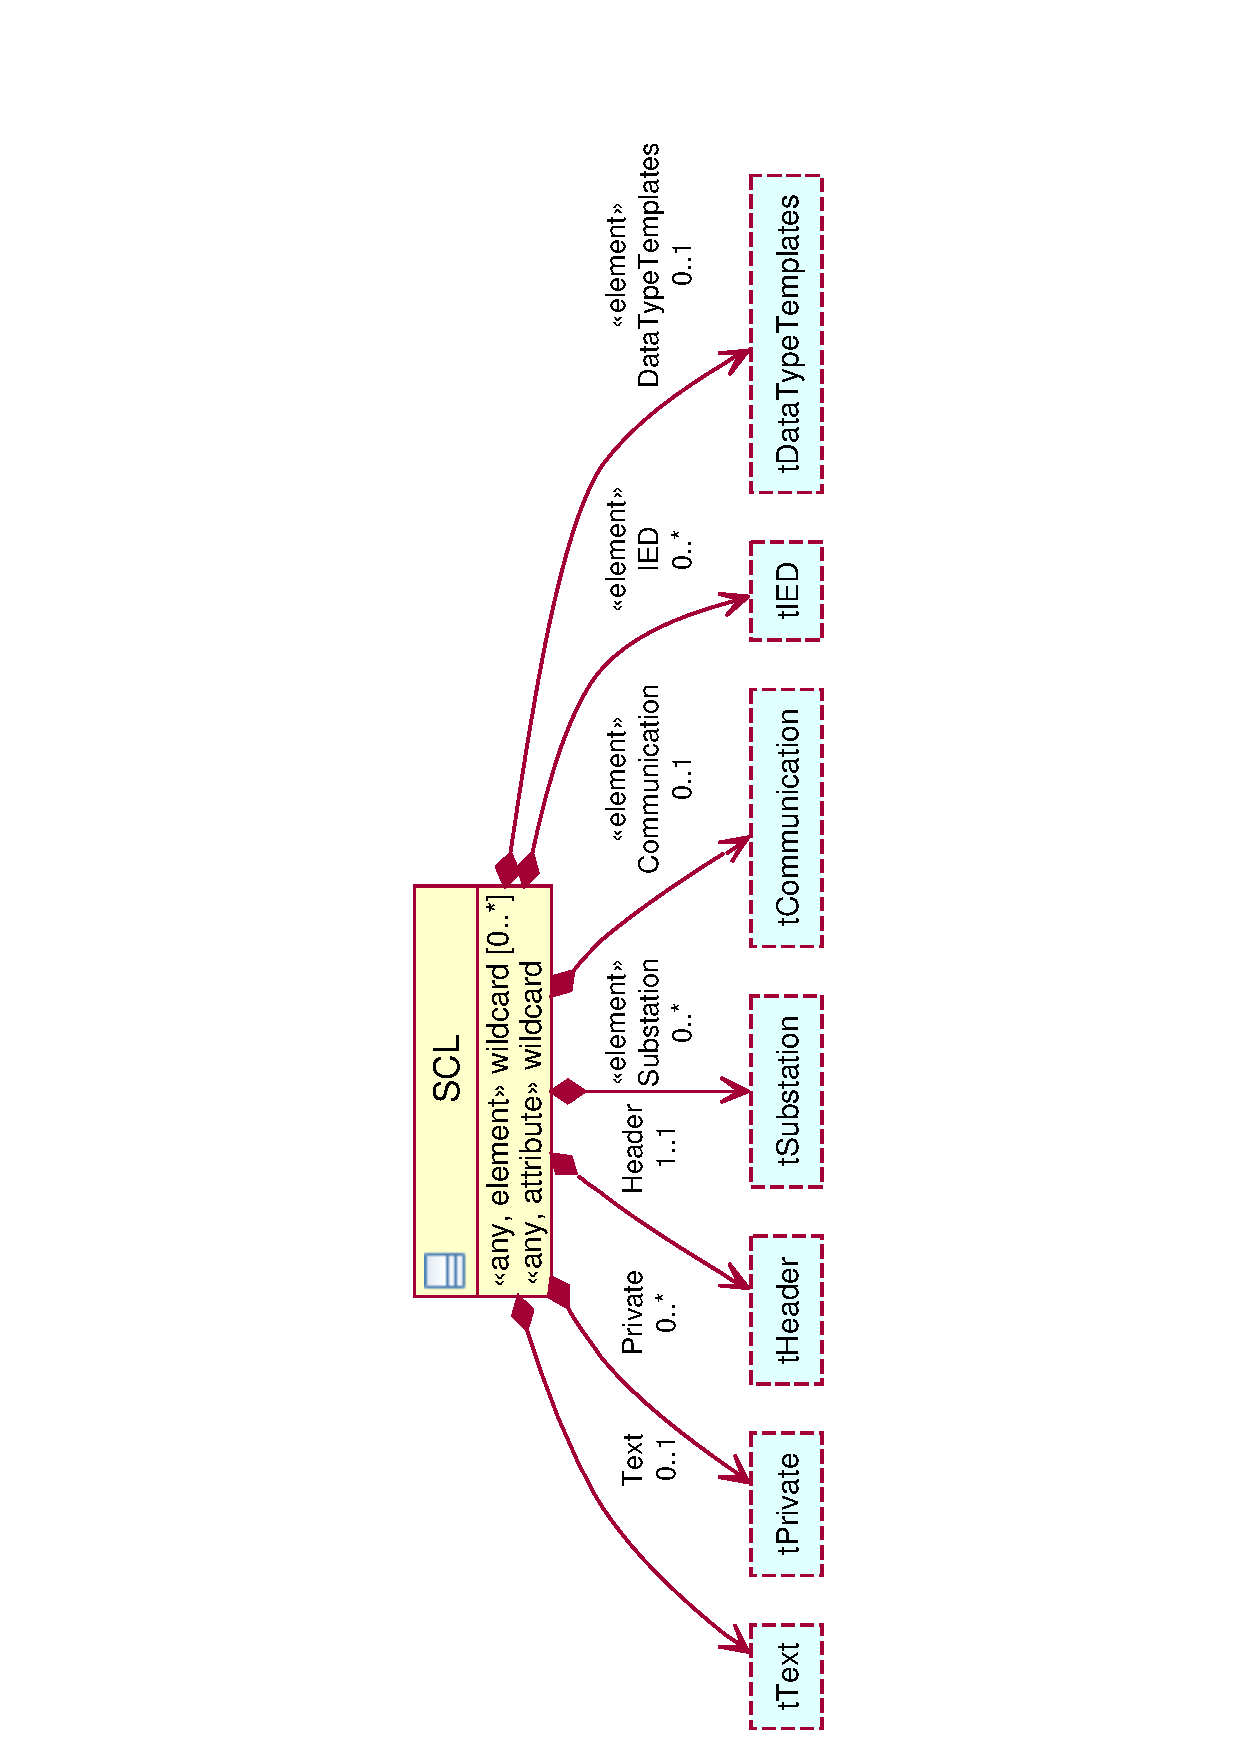
\includegraphics[
						angle=-90,	  
	  					width=1.0\textwidth 
	  				   ]{chapters/ch-scl/figures/SCL-uml-Deept2}
	  \caption{SCL object model}  
	  \label{fig:pdf-SCL-uml-deept2}
	\end{figure}
\end{center}
 
%\begin{landscape}
%\end{landscape}


Basically, it is composed by: 
\todo[color=green!40]{61850, parte6, cl6.1, \textparagraph 5}



\begin{itemize}
  \item The substation model: the object model of the primary power structure
  		(a instance of tSubstation) with their designations structured according to 
  		IEC 61346-1 \cite{IEC61346-1:1996}. 
  \item The communication model: the object model of the IED 
  		communication system configuration, 
  		i.e.,
  		the the networks, subnetworks, ports informations
  		\todo[color=green!40]{61850, parte6, cl6.1, \textparagraph 5},
  		the communication connection relations of IEDs to 
  		subnetworks, the routing for another subnetworks informations, 
  		and clocks configuration information and locations for 
  		time synchronisation (the gateways are not considered here, 
  		a gateway has to be modelled as another IED)
  		\todo[color=green!40]{61850, parte6, cl6.1, \textparagraph 8}.
  \item The product model: Contains the IEDs objects and their 
  		logical node implementations. 
  \todo[inline]{averiguar la funcion del DataTypeTemplates para agregar aca
  si corresponde}
\end{itemize}

All the structures are derived from differents 
parts depicted in the figure \ref{fig:pdf-SCL-uml-deept2}. 
In this figure, each class represent the top level 
of their structure, e.g., the substation class 
mentioned here has voltage levels, 
connectivity nodes and tranformers.   
Theses classes are completely decoupled 
(the most notable decoupling are the diferentiation of  
Logical node classes on the 
IED -t\gls{LN}- and Substation -t\gls{LNode}- structure), 
allowing the separation of the \gls{SCL} development 
by the differents engineering process 
described in the section \ref{sec:SCL-engineering-parts}.


The \gls{SCL} relationship are based in a 
ring \gls{O-O} architecture between Substation,
IED, Header, Communication, and DataTypeTemplate classes,
and it are based in a hierarchical structure under each of the 
mentioned classes.



\subsection{SCL modelling steps}
\todo[inline]{esta seccion la dejo pendiente,
debo escribirlo con detenimiento para 
que queden en concordancia la 
figura \ref{fig:pdf-SCL-uml-deept2} 
y lo que tengo escrito en esta seccion}

The figure \ref{fig:SCL-development-process} 
show the detailed SAS engineering 
process depicted with 
the autor interpretation of the step 
mentioned in the standard by 
using an \gls{UML} secuence diagram.

The more usual approach for the \gls{SAS} description 
with \gls{SCL} begin with the 
single line drawing process where the 
substation topology are defined using a 
system configurator tool. The system configurator tool, 
described in the section \ref{sec:ch-scl--System-configurator-tool}, 
creates the \gls{SSD} file containing the \glspl{LNode}
and their allocation in the substation. 
The class diagram provided by the author 	 
are based on the \gls{SCL} 
\gls{XSD}['s] of the substation. (figures  
\ref{fig:pdf-SCL-uml-substation-Deept2} and 
\ref{fig:pdf-SCL-uml-substation-Deept2-inherited}).

The \glspl{LNode} objects SCL models 
(from the substation section) is used to map 
the \gls{IED} object model references  
(figure \ref{}
\todo{apuntar a label{fig:pdf-SCL-uml-IED-Deept2}}) 
that describes 
the \gls{IED} objects are used to mapping 
\todo{terminar bien este parrafo\ldots}


\todo[inline]{a este le falta
expandir la clase correspondiente hasta que muestre el transformador }
\begin{figure}
  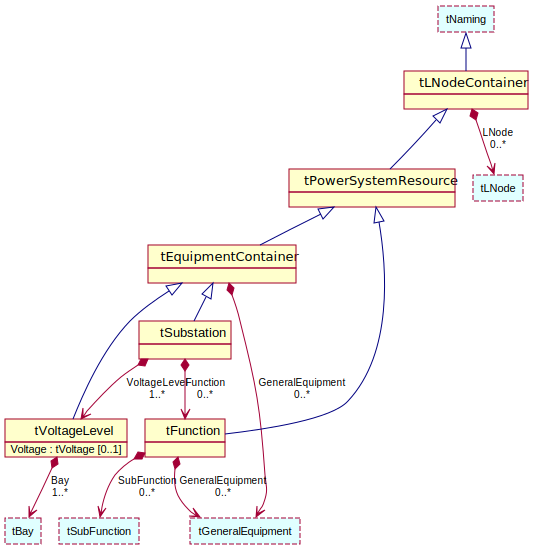
\includegraphics[width=1.0\linewidth]{chapters/ch-scl/figures/SCL-uml-substation-Deept2}
  \caption{SCL Substation class diagram with heritance 
  details} 
  \label{fig:pdf-SCL-uml-substation-Deept2}
\end{figure}


\todo[inline]{a este le valta
  expandir la clase correspondiente hasta que muestre el transformador }
\begin{figure}
  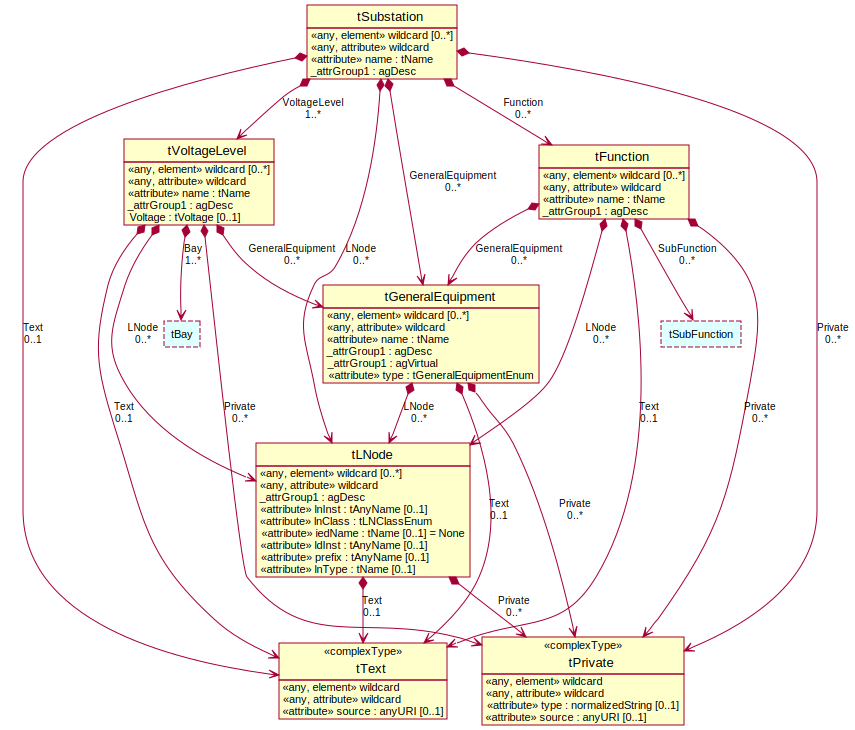
\includegraphics[width=1.0\linewidth]{chapters/ch-scl/figures/SCL-uml-substation-Deept2-inherited}
  \caption{SCL Substation class diagram inherited  }
  \label{fig:pdf-SCL-uml-substation-Deept2-inherited}
\end{figure}


\begin{figure}
  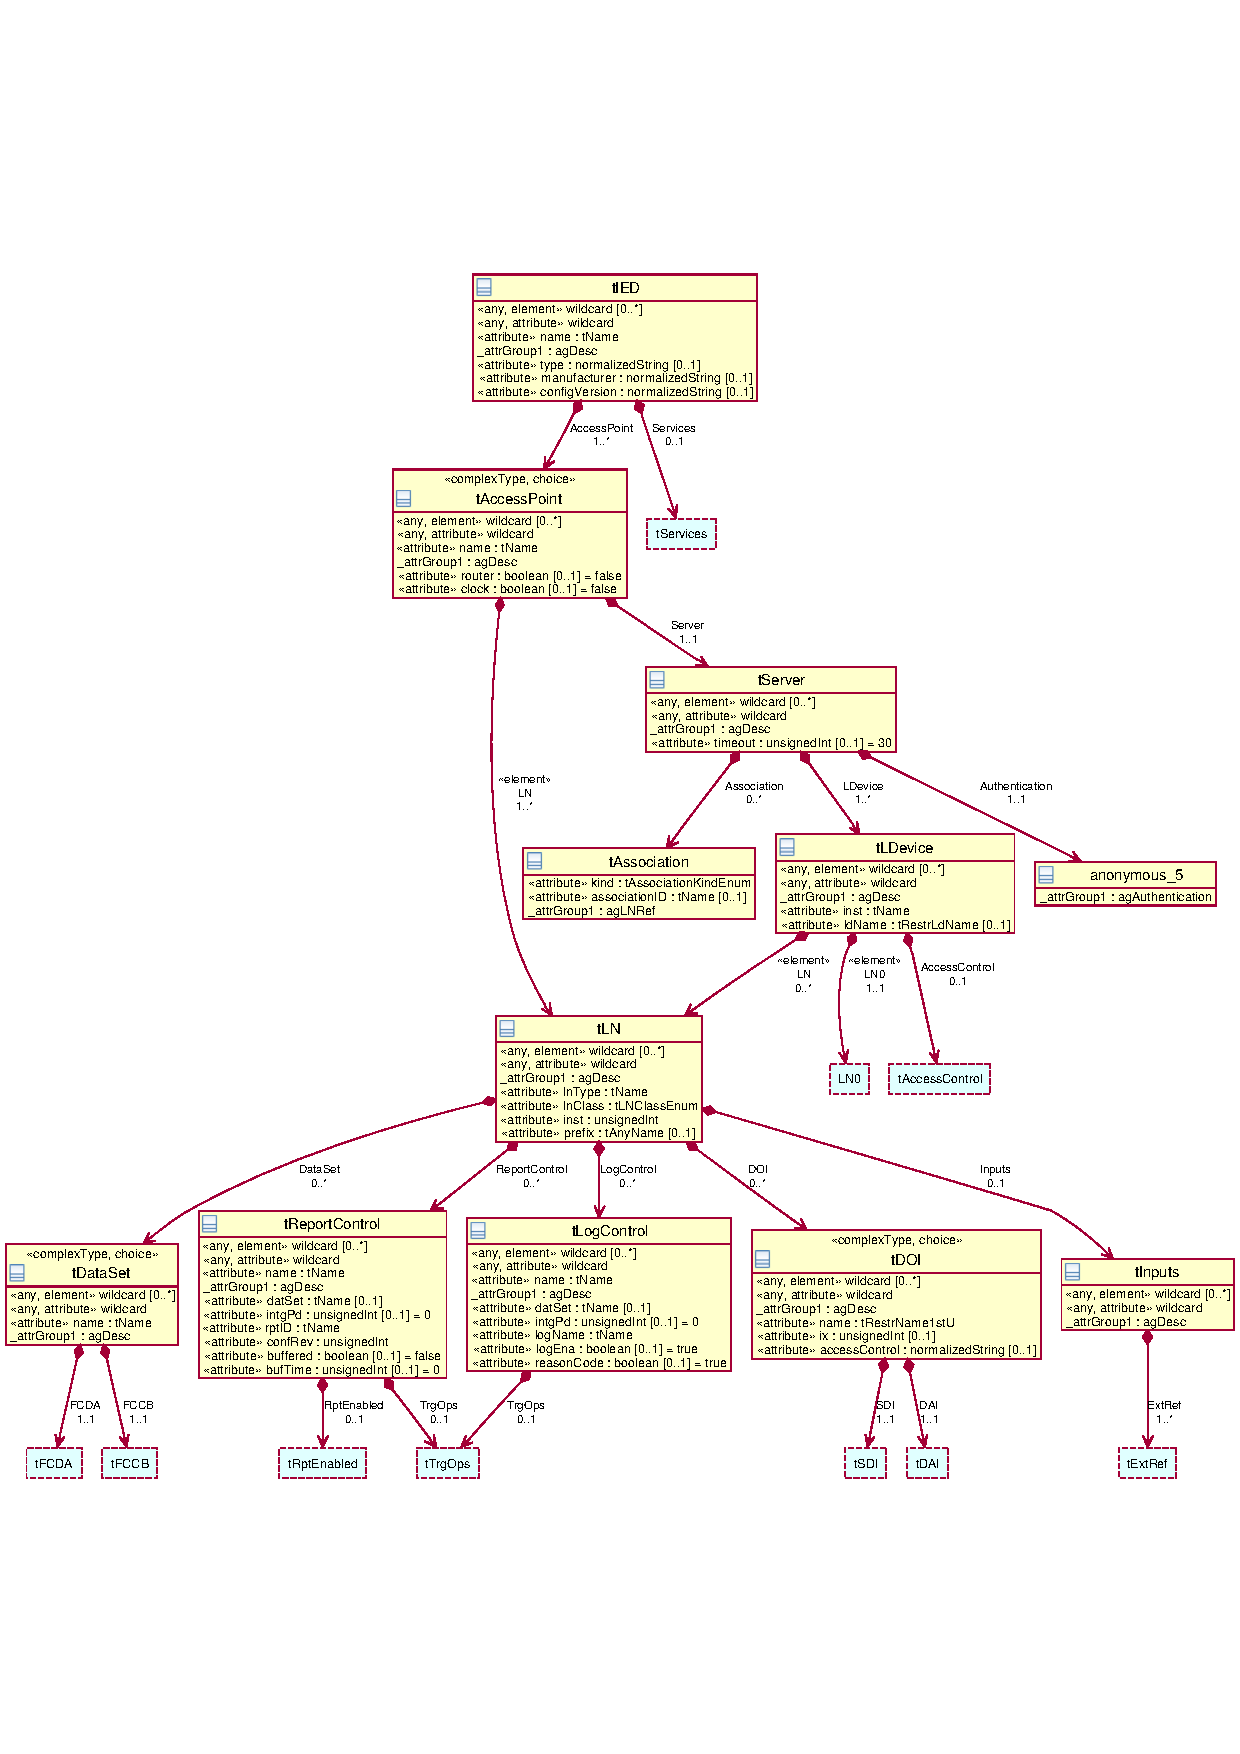
\includegraphics[width=1.0\linewidth]{chapters/ch-scl/figures/SCL-uml-IED-Deept2-inherited}
  \caption{SCL Substation class diagram inherited  }
  \label{fig:pdf-SCL-uml-IED-Deept2-inherited}
\end{figure}

%\begin{figure}
% 
%  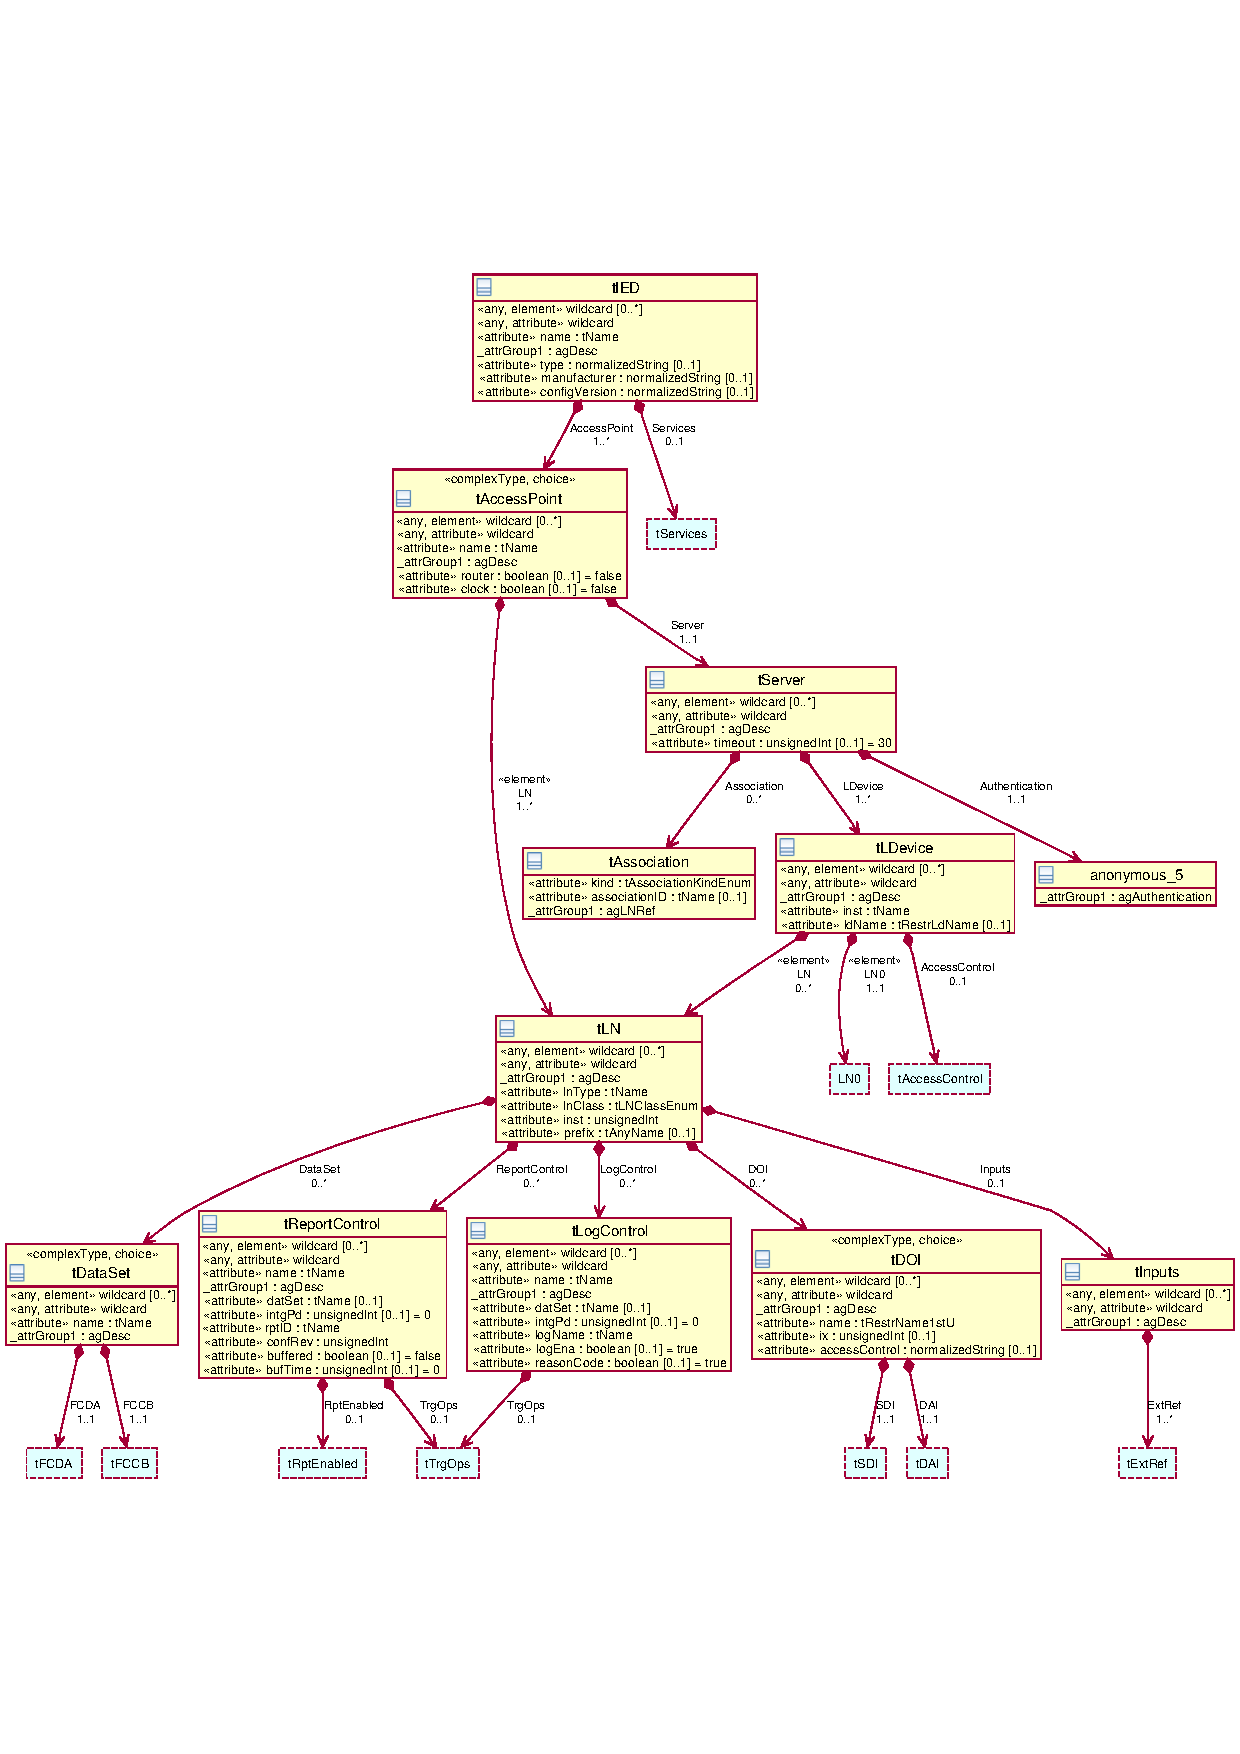
\includegraphics[width=1.0\linewidth]{chapters/ch-scl/figures/SCL-uml-IED-Deept2-inherited}
%  \caption{SCL Substation class diagram inherited  }
%  \label{fig:pdf-SCL-uml-IED-Deept2}
%\end{figure}
\missingfigure[color=green!40]{aqui falta el uml del IED con detalles de
herencia}



\todo[inline]{debo agregar aca la explicacion de los demas modelos
descriptos mediance los XSDs, pues esos tres 
items que menciona la norma son solo los mas
importantes, pero no da para entender y saber leer 
los archivos scl sabiendo solo eso. Los tres items mencionados arriba
son solo la base. Falta principalmente el DATypeTemplate
que corresponden a los objetos a serializar correspondientes 
a las instancias de las clases de la parte 7-x}



\begin{landscape}
	\begin{figure}
	  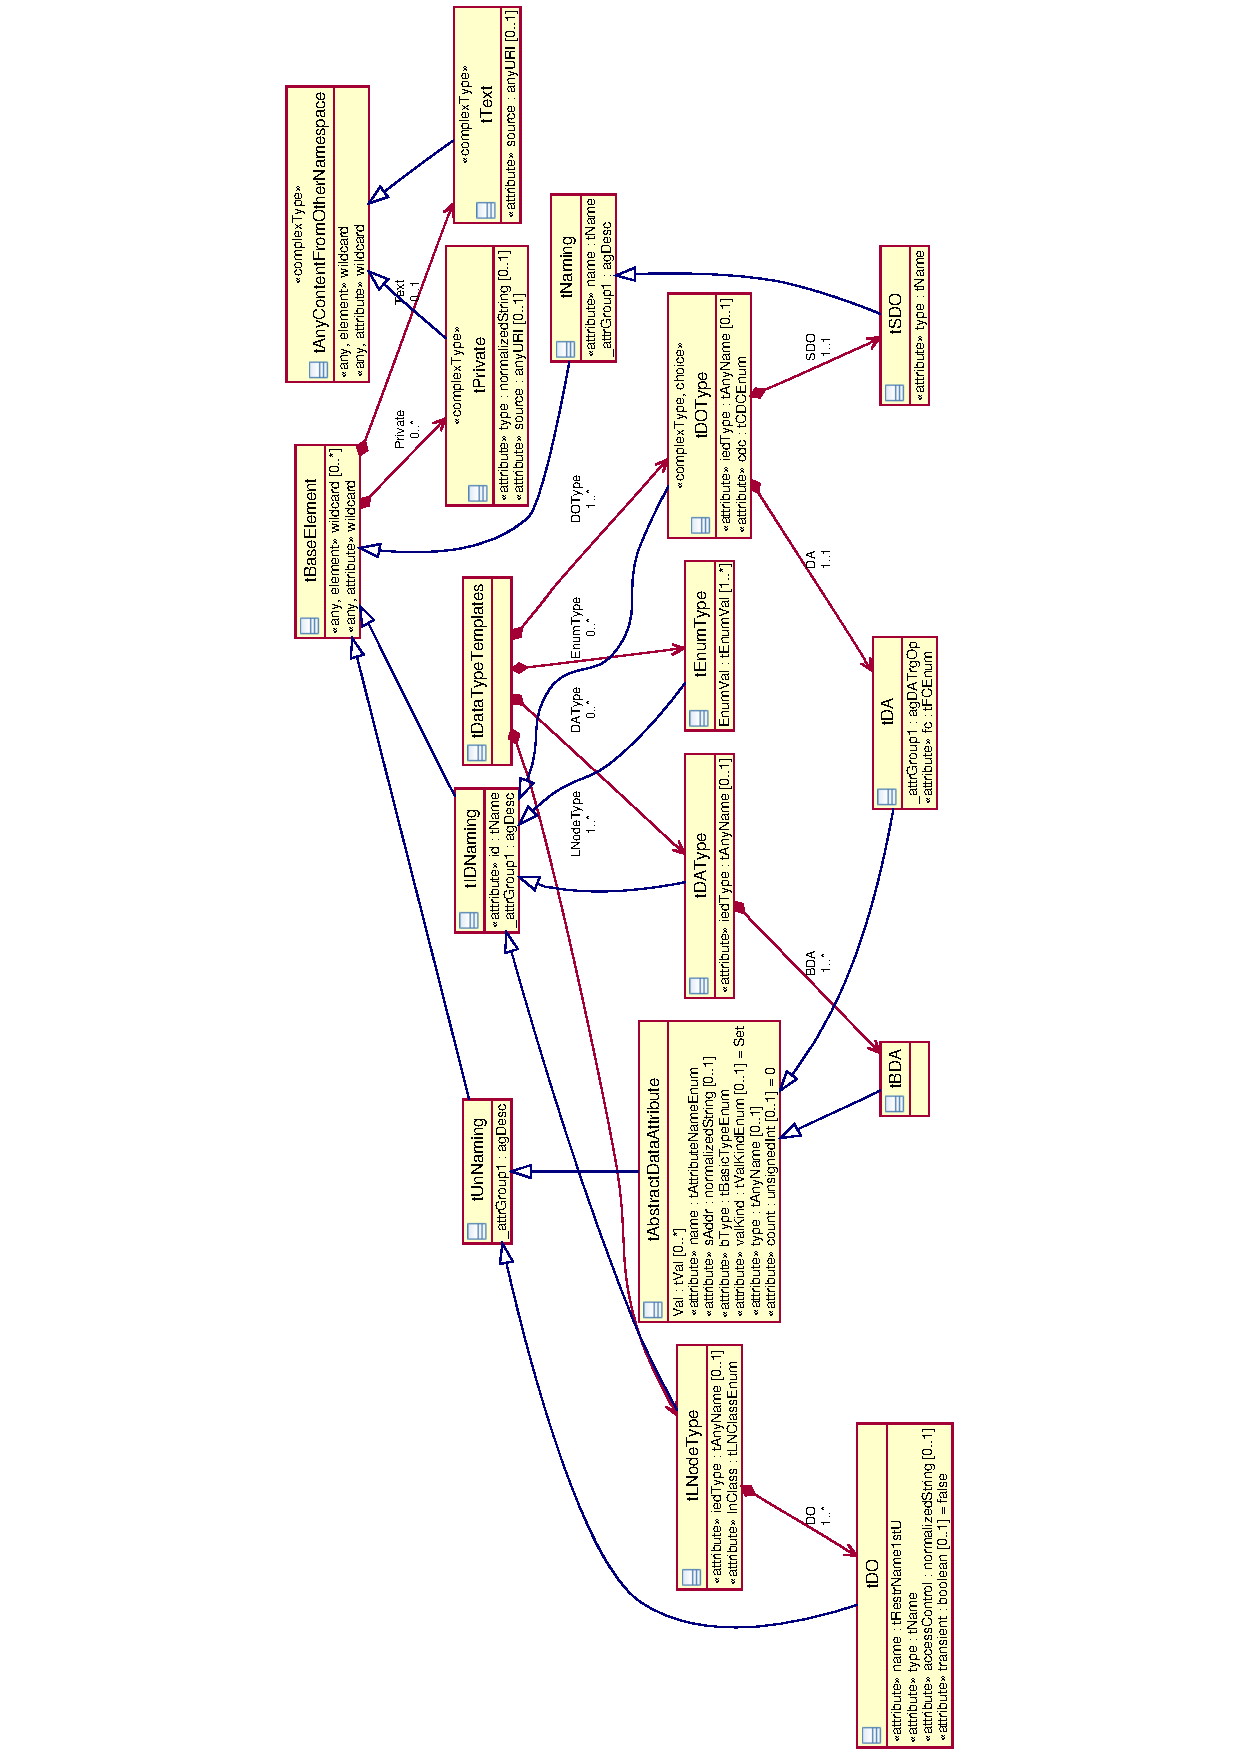
\includegraphics[angle=-90, width=1.0\linewidth]{chapters/ch-scl/figures/SCL-uml-DATypeTemplate-Deept2}
	  \caption{DAType class diagram template with heritance details}  
	  \label{fig:pdf-SCL-uml-DATypeTemplate-Deept2}
	\end{figure}
\end{landscape}

\begin{landscape}
	\begin{figure}
	  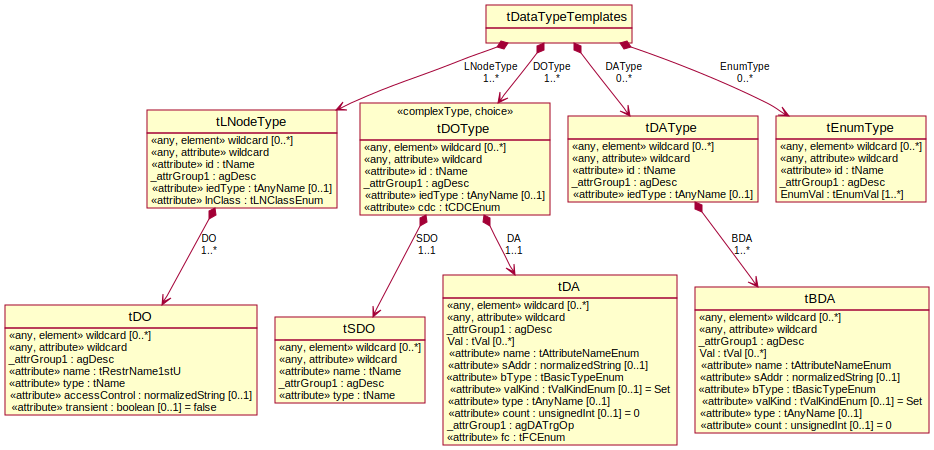
\includegraphics[angle=-90, width=1.0\linewidth]{chapters/ch-scl/figures/SCL-uml-DATypeTemplate-Deept2-inherited}
	  \caption{DAType class diagram template inherited}  
	  \label{fig:pdf-SCL-uml-DATypeTemplate-Deept2-inherited}
	\end{figure}
\end{landscape}

\begin{landscape}
	\begin{figure}
	  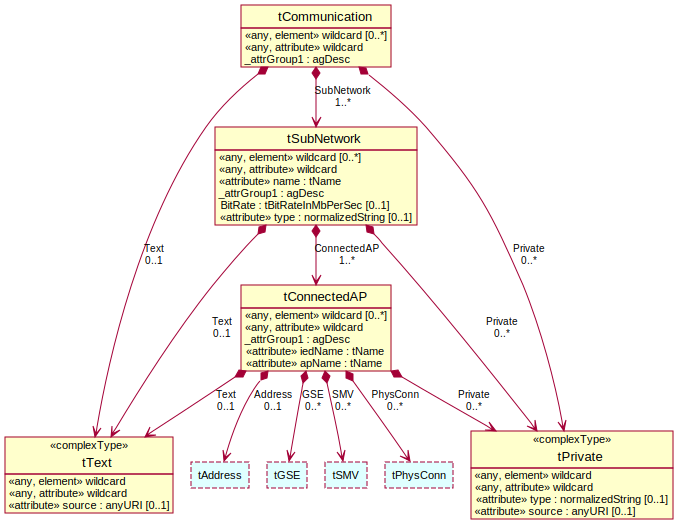
\includegraphics[angle=-90, width=1.0\linewidth]{chapters/ch-scl/figures/SCL-uml-communication-Deept3}
	  \caption{SCL Communication class diagram}  
	  \label{fig:pdf-SCL-uml-communication-Deept3}
	\end{figure}
\end{landscape}


The UML of the 
figure \ref{fig:SCL-uml-Resumen} 
is a resume of
the SCL model, where is evident the 
key importance of the Logical Node for  
the information topology description (see 
the composition of the Substation 
class). The Logical Node is  
the transition object to 
connect the diferent structures of the SAS 
\todo[color=green!40]{61850, parte6, cl6.1, \textparagraph 9} 
that are defined by IEC 61341-1 \cite{IEC61346-1:1996}.


\begin{landscape}

\begin{figure}
  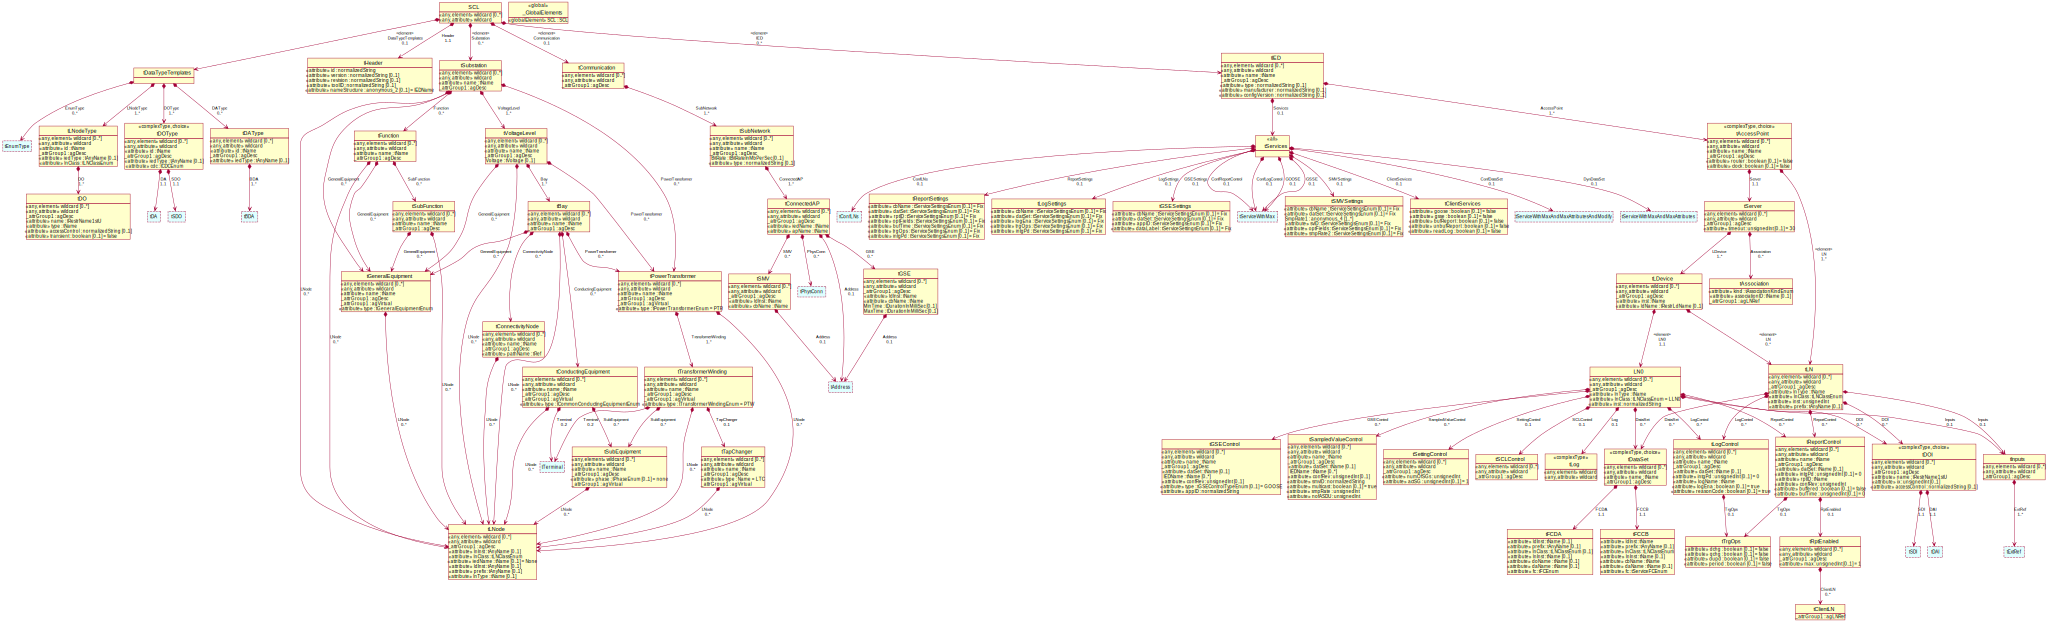
\includegraphics[angle=-90,
  width=1.0\linewidth]{chapters/ch-scl/figures/SCL-uml-Resumen-inherited}
  \caption{Resume of SCL shema represented by a UML class diagram}
  \label{fig:SCL-uml-Resumen}
\end{figure}
\end{landscape}


\renewcommand{\glossaryname}{Glosario}
\renewcommand{\listtablename}{�ndice de tablas} 
\renewcommand{\tablename}{Tabla} 


\thispagestyle{empty}

\vspace*{-1cm}
{\bf
\begin{center}
\large
\hspace*{0cm}\large Universidad Nacional del Este \\
\hspace*{0cm}\large Facultad Polit\'ecnica \\
\hspace*{0cm}\large Carrera de Ingenier\'ia El\'ectrica\\
\end{center}
}

\vspace{0.0cm}
{
\noindent
\begin{center}
\Large \bf Dise�o del modelo IEC 61850 del regulador de velocidad de una unidad generadora t�pica de la Central Hidroel�ctrica Itaipu.
\end{center}
}

\begin{minipage}[t]{-1cm}
\end{minipage}\\[0cm]
{
\flushright\begin{minipage}[b]{10cm}
\large%Trabajo final de grado presentado a la Facultad Polit\'ecnica de la  \textit{Universidad Nacional del Este - U.N.E}, como requisito parcial para la obtenci\'on del grado de Ingeniero Electricista.
Presentado a la Facultad Polit\'ecnica en cumplimiento parcial de los requisitos para obtener el grado de Ingeniero Electricista en la Universidad Nacional del Este.
\end{minipage}\\[0cm]
}
\vspace{1cm}
{ 
\begin{center}
\small por\\
\textbf{\Large David Daniel P\'erez Sosa}
\end{center}
\vspace{0.5cm}   %%%%%2
Orientador: Prof. Ing. Enrique Ram�n Chaparro Viveros, D.Sc.\\
Co-orientador: Prof. Ing. Juan Manuel Ramirez Duarte.\\
Co-orientador: Prof. Ing. Rodrigo Andr�s Ramos, M.Sc.\\
Co-orientador: Prof. Ing. Ladislao Aranda Arriola, M.Sc. \\
}%\\[6mm]

\vspace{1.0cm}   %%%%%2
\begin{center}
{\large {\bf Ciudad del Este, Alto Paran\'a, Paraguay}\\
Diciembre de 2010}\\
\small \copyright David Daniel P�rez Sosa, 2010 - 2012. Todos los derechos reservados.
\end{center}
\newpage
%
\hyphenation{}

% Ficha Catalogr\'afica
\hspace{8em}\fbox{
\begin{minipage}{10cm}
\\
David Daniel P\'erez Sosa

\hspace{2em} Dise�o del modelo IEC 61850 del regulador de velocidad de una unidad generadora t�pica de la Central Hidroel�ctrica Itaipu


\hspace{2em} \pageref{LastPage} p\'aginas

\hspace{2em}Disertaci\'on (Grado) - Facultad Polit\'ecnica - Universidad Nacional del Este. Departamento de Ingenier\'ia El\'ectrica.

\begin{enumerate}
\item Norma IEC 61850.
\item Automatizaci\'on de Centrales Hidroel\'ectricas.
\end{enumerate}

Universidad Nacional del Este. Facultad Polit\'ecnica. \\Departamento de Ingenier\'ia El\'ectrica.
\end{minipage}
}
%\newpage
%%%%%%%%%%%%%%%%%%%%%%%%%%%%%%%%%%%%%%%%%%%%%%%%%%%%
%\begin{minipage}{10cm}

%\end{minipage}
%%%%%%%%%%%%%%%%%%%%%%%%%%%%%%%%%%%%%%%%%%%%%%%%%%%%
\thispagestyle{empty}
\newpage

Certifico que el presente Trabajo Final de Grado titulado  ``Dise�o del modelo IEC 61850 del regulador de velocidad de una unidad generadora t�pica de la Central Hidroel�ctrica Itaipu'' ha sido realizado por David Daniel P\'erez Sosa, bajo mi orientaci\'on.

El mismo es producto del esfuerzo personal y original del graduando, de lo que doy fe y en mi opini\'on re\'une los m\'eritos para su aprobaci\'on y defensa ante la mesa examinadora designada por la instituci\'on.


\begin{flushright}
Ciudad del Este,.........de..................................de 2012
\end{flushright}

\vspace*{1cm}
{\raggedleft
\begin{minipage}[t]{16cm}
\setlength{\baselineskip}{0.25in}
\begin{center}
...............................................................................
 
    Prof. Ing. Enrique R. Chaparro V., D.Sc.
		
		Orientador de Trabajo Final de Grado
\end{center}
\end{minipage}\\[1cm]
}

Nosotros, los miembros de la Mesa Examinadora del Trabajo Final de Grado de la carrera de Ingenier\'ia El\'ectrica de la Facultad Polit\'ecnica de la Universidad Nacional del Este, hacemos constar que el presente Trabajo Final de Grado titulado ``ise�o del modelo IEC 61850 del regulador de velocidad de una unidad generadora t�pica de la Central Hidroel�ctrica Itaipu'' ha sido evaluado en forma y evaluado por esta Mesa, la que por .........................................ha resuelto conceder la calificaci\'on ...................................

\begin{flushright}
Ciudad del Este,.........de..................................de 2012
\end{flushright}


\begin{table}[h]
	\centering
		\begin{tabular}{cc}
		& \\
		
.........................................................&........................................................\\
Prof. Ing.  &Prof. Ing. \\
Miembro de la Mesa Examinadora&Miembro de la Mesa Examinadora\\
&    \\
&    \\
.........................................................& \\
Prof. Ing.&    \\
Miembro de la Mesa Examinadora &
		\end{tabular}
\end{table}



%\newpage
\thispagestyle{empty}
%%%%%%%%%%%%%%%%%%%%%%%%%%%%%%%%%%%%%%%%%%%%%%%%%%%%
\begin{minipage}{10cm}

\end{minipage}
%%%%%%%%%%%%%%%%%%%%%%%%%%%%%%%%%%%%%%%%%%%%%%%%%%%%

% -*-latex-*-
% $Log: cover.tex,v $
% Revision 1.8  2008/05/13 15:02:15  jdreed
% Degree month is June, not May.  Added note about prevdegrees.
% Arthur Smith's title updated
%
% Revision 1.7  2001/02/08 18:53:16  boojum
% changed some \newpages to \cleardoublepages
%
% Revision 1.6  1999/10/21 14:49:31  boojum
% changed comment referring to documentstyle
%
% Revision 1.5  1999/10/21 14:39:04  boojum
% *** empty log message ***
%
% Revision 1.4  1997/04/18  17:54:10  othomas
% added page numbers on abstract and cover, and made 1 abstract
% page the default rather than 2.  (anne hunter tells me this
% is the new institute standard.)
%
% Revision 1.4  1997/04/18  17:54:10  othomas
% added page numbers on abstract and cover, and made 1 abstract
% page the default rather than 2.  (anne hunter tells me this
% is the new institute standard.)
%
% Revision 1.3  93/05/17  17:06:29  starflt
% Added acknowledgements section (suggested by tompalka)
% 
% Revision 1.2  92/04/22  13:13:13  epeisach
% Fixes for 1991 course 6 requirements
% Phrase "and to grant others the right to do so" has been added to 
% permission clause
% Second copy of abstract is not counted as separate pages so numbering works
% out
% 
% Revision 1.1  92/04/22  13:08:20  epeisach

% NOTE:
% These templates make an effort to conform to the MIT Thesis specifications,
% however the specifications can change.  We recommend that you verify the
% layout of your title page with your thesis advisor and/or the MIT 
% Libraries before printing your final copy.
\title{An Optimizing Compiler for Low-Level Floating Point Operations}

\author{Lucien William Van Elsen}
% If you wish to list your previous degrees on the cover page, use the 
% previous degrees command:
%       \prevdegrees{A.A., Harvard University (1985)}
% You can use the \\ command to list multiple previous degrees
%       \prevdegrees{B.S., University of California (1978) \\
%                    S.M., Massachusetts Institute of Technology (1981)}
\department{Department of Electrical Engineering and Computer Science}

% If the thesis is for two degrees simultaneously, list them both
% separated by \and like this:
% \degree{Doctor of Philosophy \and Master of Science}
\degree{Bachelor of Science in Computer Science and Engineering}

% As of the 2007-08 academic year, valid degree months are September, 
% February, or June.  The default is June.
\degreemonth{June}
\degreeyear{1990}
\thesisdate{May 18, 1990}

%% By default, the thesis will be copyrighted to MIT.  If you need to copyright
%% the thesis to yourself, just specify the `vi' documentclass option.  If for
%% some reason you want to exactly specify the copyright notice text, you can
%% use the \copyrightnoticetext command.  
%\copyrightnoticetext{\copyright IBM, 1990.  Do not open till Xmas.}

% If there is more than one supervisor, use the \supervisor command
% once for each.
\supervisor{William J. Dally}{Associate Professor}

% This is the department committee chairman, not the thesis committee
% chairman.  You should replace this with your Department's Committee
% Chairman.
\chairman{Arthur C. Smith}{Chairman, Department Committee on Graduate Theses}

% Make the titlepage based on the above information.  If you need
% something special and can't use the standard form, you can specify
% the exact text of the titlepage yourself.  Put it in a titlepage
% environment and leave blank lines where you want vertical space.
% The spaces will be adjusted to fill the entire page.  The dotted
% lines for the signatures are made with the \signature command.
\maketitle

% The abstractpage environment sets up everything on the page except
% the text itself.  The title and other header material are put at the
% top of the page, and the supervisors are listed at the bottom.  A
% new page is begun both before and after.  Of course, an abstract may
% be more than one page itself.  If you need more control over the
% format of the page, you can use the abstract environment, which puts
% the word "Abstract" at the beginning and single spaces its text.

%% You can either \input (*not* \include) your abstract file, or you can put
%% the text of the abstract directly between the \begin{abstractpage} and
%% \end{abstractpage} commands.

% First copy: start a new page, and save the page number.
\cleardoublepage
% Uncomment the next line if you do NOT want a page number on your
% abstract and acknowledgments pages.
% \pagestyle{empty}
\setcounter{savepage}{\thepage}
\begin{abstractpage}
% $Log: abstract.tex,v $
% Revision 1.1  93/05/14  14:56:25  starflt
% Initial revision
% 
% Revision 1.1  90/05/04  10:41:01  lwvanels
% Initial revision
% 
%
%% The text of your abstract and nothing else (other than comments) goes here.
%% It will be single-spaced and the rest of the text that is supposed to go on
%% the abstract page will be generated by the abstractpage environment.  This
%% file should be \input (not \include 'd) from cover.tex.
In this thesis, I designed and implemented a compiler which performs
optimizations that reduce the number of low-level floating point operations
necessary for a specific task; this involves the optimization of chains of
floating point operations as well as the implementation of a ``fixed'' point
data type that allows some floating point operations to simulated with integer
arithmetic.  The source language of the compiler is a subset of C, and the
destination language is assembly language for a micro-floating point CPU.  An
instruction-level simulator of the CPU was written to allow testing of the
code.  A series of test pieces of codes was compiled, both with and without
optimization, to determine how effective these optimizations were.

\end{abstractpage}

% Additional copy: start a new page, and reset the page number.  This way,
% the second copy of the abstract is not counted as separate pages.
% Uncomment the next 6 lines if you need two copies of the abstract
% page.
% \setcounter{page}{\thesavepage}
% \begin{abstractpage}
% % $Log: abstract.tex,v $
% Revision 1.1  93/05/14  14:56:25  starflt
% Initial revision
% 
% Revision 1.1  90/05/04  10:41:01  lwvanels
% Initial revision
% 
%
%% The text of your abstract and nothing else (other than comments) goes here.
%% It will be single-spaced and the rest of the text that is supposed to go on
%% the abstract page will be generated by the abstractpage environment.  This
%% file should be \input (not \include 'd) from cover.tex.
In this thesis, I designed and implemented a compiler which performs
optimizations that reduce the number of low-level floating point operations
necessary for a specific task; this involves the optimization of chains of
floating point operations as well as the implementation of a ``fixed'' point
data type that allows some floating point operations to simulated with integer
arithmetic.  The source language of the compiler is a subset of C, and the
destination language is assembly language for a micro-floating point CPU.  An
instruction-level simulator of the CPU was written to allow testing of the
code.  A series of test pieces of codes was compiled, both with and without
optimization, to determine how effective these optimizations were.

% \end{abstractpage}

\cleardoublepage

\section*{Acknowledgments}

This is the acknowledgements section.  You should replace this with your
own acknowledgements.

%%%%%%%%%%%%%%%%%%%%%%%%%%%%%%%%%%%%%%%%%%%%%%%%%%%%%%%%%%%%%%%%%%%%%%
% -*-latex-*-


\pagestyle{plain}
  % -*- Mode:TeX -*-
%% This file simply contains the commands that actually generate the table of
%% contents and lists of figures and tables.  You can omit any or all of
%% these files by simply taking out the appropriate command.  For more
%% information on these files, see appendix C.3.3 of the LaTeX manual. 


\tableofcontents
\newpage
\printglossaries
%\printglossary[title={Acronyms}]
\newpage
\listoffigures
\newpage
\listoftables


  
%\chapter*{Annotations}

Auxiliary chapter (not is part of this document content).
En esta parte explico sobre la plataforma latex que utilizo, sobre la
sistematizaci\'on que utilizo para redactar este documento, por ejemplo, que
significan los comentarios que hago con el comando TODO, etc.

\section{Convenci\'on de colores para los comentarios hechos en este documento}
	Un comentario de color 
	\emph{NARANJADO}
	\todo{Ejemplo}   
	indica las cosas que me faltan hacer.\\

	Un comentario de color 
	\emph{VERDE CLARO}
	\todo[color=green!40]{green!40}
	indica en que parte de la norma IEC 61850 se est\'a utilizando la teor\'ia
	comentada. Indica la relaci\'on del contenido bibliogr\'afico de conceptos con
	la norma. 
	Un ejemplo de uso de este tipo de comentarios en mi trabajo:
	En redes, cuando hablo de un concepto, por ejemplo, \emph{network
	reliability}, eso se habla en la norma, en la parte IEC 61850-xx, entonces yo
	indico en el comentario de que ese concepto se menciona en la tesis. 
	Esto es \'util para mi pues me sirve para justificar por que inclu\'i la 
	descripci\'on de alg\'un concepto en el trabajo, principalmente en el marco
	te\'orico, que utilizar\'e para describir todos los conocimientos necesarios
	para abordar la norma (por ejemplo: Redes, Programaci\'on orientada a
	objetos, UML).\\
	
	Los colores en \emph{LILA}
	\todo[inline, color=blue!50!red!50]{color=blue!50!red!50}
	indican peque\~nas variaciones de palabras que podr\'ia hacer pero no son de
	alta prioridad ni obligatorias de corregir (a mi punto de vista), pero
	la modificaci\'on de las partes comentadas mejorar\'ia la redacci\'on del
	texto, o bien explican por que hice esas mejoras o ubique, redacte, 
	o modifique de esa 	manera un determinado parrafo.
	

\section{Im\'agenes por agregar al trabajo}
	Por convenci\'on, utilizar\'e la siguiente imagen
	\missingfigure[color=green!40]{prueba del comando de falta de figura}
	para indicar de que est\'a faltando incluir la imagen en este lugar. Durante
	el proceso de redacci\'on se ir\'a agregando el contenido faltante




%%Agrega la lista de cosas (comentarios) que hay que hacer
\listoftodos


%\listoftodos

\chapter{Informaciones generales}
\label{ch:informaciones-generales}
%\include{chapters/sample}
%\section{Introduction}
%For comming\ldots
\section{Introducci�n}

La energ�a en todo el mundo mueve por lo menos siete billones de d�lares
anuales, y es un negocio en expansi�n, afectando profundamente nuestra econom�a,
sociedad y entorno \cite{Dukert:2009ab}, debido a esto, existe una constante
investigaci�n en el sector y han surgido nuevas tecnolog�as y normas 
que est�n llev�ndonos hacia la nueva era de los sistemas de potencia:
los sistemas el�ctricos inteligentes (en ingl�s, \emph{Smart Grids}).
En este contexto, la automatizaci�n y el tratamiento de la informaci�n de los
sistemas de potencia se constituyen como infraestructuras estrat�gicas en el
desarrollo de los pa�ses, muchos de los cuales ya han comenzado el proceso de
actualizaci�n tecnol�gica.

Este proceso de actualizaci�n tecnol�gica del sector el�ctrico est� siendo
proyectado y ejecutado a nivel mundial, introduci�ndose nuevos paradigmas
en el proceso de ingenier�a de los sistemas el�ctricos, apoyado en nuevos
pilares que resaltan por su sofisticaci�n, integraci�n
multidisciplinar, innovaci�n y pueden atender las exigencias globales del
consumo de energ�a, ayudando al ser humano en la construcci�n de un mundo
mejor.

En la automatizaci�n de los sistemas de energ�a se destaca el proceso de
digitalizaci�n de la informaci�n gracias a la amplia utilizaci�n de 
dispositivos basados en uno o varios microprocesadores
\cite{Santoso:2000} integrados llamados \Glspl{IED},
los cuales aprovechan una serie de tecnolog�as de redes de comunicaci�n que
son adecuadas para cubrir las necesidades de monitoreo, supervisi�n,
automatizaci�n, control y protecci�n de los sistemas el�ctricos.

El intercambio de informaci�n entre \Glspl{IED} de diferentes fabricantes se ha
vuelto muy complejo, costoso, y a veces imposible, es por ello que la
industria ha comenzado a desarrollar normas internacionales en forma
colaborativa, y as� conseguir interoperabilidad, confiabilidad
y mayor calidad en el intercambio de informaci�n dentro del sistema de
automatizaci�n de los procesos el�ctricos de potencia.

La norma internacional IEC 61850 \emph{``Comunication Networks and Systems in
Substations''} provee soporte para una interoperabilidad a prueba
de futuro en el intercambio de la informaci�n a trav�s de la especificaci�n de: 
	\begin{itemize}
	  \item un modelo orientado a objetos y sem�ntico de toda la estructura de la informaci�n,
	  \item m�todos de intercambio de la informaci�n con interfaces permanentes y bien definidas,
	  \item mapeo de estas interfaces a protocolos de comunicaci�n acordes al estado del arte de las tecnolog�as de comunicaci�n,
	  \item y un lenguaje de configuraci�n de los IEDs y de las redes de comunicaci�n de los procesos el�ctricos.
	\end{itemize}

La norma IEC 61850, en la actualidad, no se enfoca �nicamente a subestaciones,
tambi�n es aplicable y extensible para satisfacer las necesidades 
de comunicaci�n de casi la
totalidad de la cadena de suministro de energ�a, entre los cuales destacamos
los sistemas de transmisi�n, distribuci�n y generaci�n (e�lica, hidroel�ctrica
y fotovoltaica)\cite{Schwarz:2008} y 
varios proyectos pilotos tales como aplicaciones de la norma a
coches el�ctricos \cite{Germany:2009}.

La correcta utilizaci�n del modelo jer�rquico de la informaci�n especificado en
la norma IEC 61850 a trav�s de nodos l�gicos es una cuesti�n clave y debe
adaptarse a la filosof�a de la planta. Las agrupaciones de los nodos l�gicos de
forma adecuada representan funciones o equipos utilizados en los sistemas de potencia. Cada nodo l�gico provee una
lista de informaci�n bien designada y organizada. Los objetos y servicios
definidos en la parte IEC 61850--7--2 \cite{IEC61850-7-2:2003} de la norma
permiten el intercambio de esta informaci�n.

En julio del 2007 las extensiones de los nodos l�gicos a centrales
hidroel�ctricas han sido aprobadas, publicadas y est�n listas para su uso, en
el apartado IEC 61850--7--4--10: \emph{``Hydroelectric Power Plants -- Communication
for monitoring and control''}; agregando 60 nodos l�gicos y 350 Data Objects a
la serie IEC 61850 \cite{IEC61850-7-410:2007}.

Este trabajo consiste en la aplicaci�n de la norma IEC 61850, en especial de la 
elecci�n de nodos l�gicos definidos en la parte 7--4--10 -- \emph{Hydro Power Plants} y de
los servicios de comunicaci�n para la automatizaci�n del regulador de
velocidad de una unidad generadora t�pica de Itaipu, y la realizaci�n de una
propuesta al TC57 (International Electrotechnical Commission, Technical
Committee 57) para la complementaci�n o extensi�n de nodos l�gicos de la norma
que actualmente son insuficientes para las unidades generadoras de Itaipu. Este
trabajo de investigaci�n se basa en el �tem del documento \emph{``Proposta de
Temas para Monografias de Especializa\c c\~ao - Automa\c c\~ao, Controle e
Supervis\~ao do Processo El�trico Baseado na Norma  IEC 61850 -- A--4 -- Automa\c
c\~ao de Unidades Geradoras -- Modelagem Completa da Unidade Geradora''} de la
Itaipu Binacional, redactado por Marcos Fonseca Mendes, Antonio Sertich
Koehler y Ladislao Aranda Arriola, funcionarios de la Itaipu Binacional.


\section{Objetivos de la investigaci�n}
\label{sec:objetivos-investigacion}
\subsection{Objetivos generales}
Dise�ar el modelo de informaci�n y servicios de intercambio 
de informaci�n entre IEDs conformes a la norma IEC 61850 para  
las funciones de monitoreo y control
del regulador de velocidad de una unidad generadora t�pica de Itaipu.

\subsection{Objetivos espec�ficos}
	\begin{itemize}
	  \item Definir las funciones de monitoreo y control requeridas por el
	  regulador de velocidad.
	  \item Implementar en \gls{SCL} los nodos l�gicos del apartado IEC
	  61850--7--4--10 necesarios para las funciones de monitoreo 
	  y control del regulador de velocidad.
	  \item Identificar los servicios de comunicaci�n del apartado IEC 61850--7--2
	  necesarios para el regulador de velocidad de las turbinas de Itaipu.
	  \item Implementar el modelo IEC 61850 del sistema considerando sus
	  ubicaciones centralizadas y/o distribuidas en la red 
	  de automatizaci�n mediante
	  herramientas de ingenier�a adecuadas para el efecto.
	  \item Proponer la extensi�n/complementaci�n de nodos l�gicos para una
	  unidad generadora t�pica de Itaipu.
    \end{itemize}
    
\section{Justificativa}

La norma IEC 61850 cubre las necesidades
de modernizaci�n de los sistemas y redes de comunicaci�n
de subestaciones y centrales hidroel�ctricas.

La Itaipu Binacional se encuentra 
actualmente en proceso de actualizaci�n 
tecnol�gica, motivo por el cual,
el modelo IEC 61850 del sistema
de comunicaci�n del regulador de 
velocidad de una unidad generadora t�pica
de la Central Hidroel�ctrica Itaipu 
podr� ser utilizada durante el proceso de dise�o 
de especificaciones t�cnicas para la   
compra de IEDs de monitoreo y control 
de regulaci�n de velocidad 
para las turbinas de Itaipu, que
estar�n en conformidad con la norma IEC 61850.
 


%\todo[inline]{falta completar la justificativa de la investigaci�n}



% \section*{Declaraci�n de originalidad de este
trabajo de \\investigaci�n}

Yo, David Daniel P�rez Sosa, declaro que este
Trabajo Final de Grado titulado 
\emph{
Dise�o del modelo IEC 61850 del regulador de velocidad 
de una unidad generadora t�pica de la 
Central Hidroel�ctrica Itaipu
}
no contiene materiales que han sido 
publicados previamente, en forma completa
o en partes, para la obtenci�n de ning�n 
otro grado acad�mico o diploma. 

Salvo donde indico lo contrario, esta
investigaci�n es fruto de mi propio trabajo.
\\  
\\ 

\par\noindent Autor \dotfill\null\\*
  {\raggedleft David Daniel P�rez Sosa \par}


\section{T�cnicas y metodolog�a de investigaci�n}

	\subsection{Investigaci�n bibliogr�fica}
	La investigaci�n bibliogr�fica consisti�
	en el estudio de la norma IEC 61850, en especial las
	definiciones de modelos de informaci�n definidos en la parte IEC 61850--7--4--10
  	\emph{``Basic communication structure for substation and feeder equipment -- 
  	Compatible logical node classes and data classes -- Hydro Power Plants''}, 
  	de los servicios de intercambio de informaci�n para diferentes funciones 
	definidos en el apartado IEC
  	61850--7--2 \emph{``Basic communication structure for substation and feeder
  	equipment -- Abstract communication service 
  	interface (ACSI)''} \cite{IEC61850-7-2:2003}, la
  	implementaci�n de dichos servicios de comunicaci�n a trav�s de protocolos
  	especificados en la parte IEC 61850--8--1 \emph{``Specific Communication
  	Service Mapping (SCSM) Mappings to MMS (ISO 9506--1 and ISO 9506--2) and to
  	ISO/IEC 8802-- 3''} \cite{IEC61850-8-1:2004} y 
  	la configuraci�n y descripci�n
  	formal de todas ellas a trav�s del apartado IEC 61850--6 \emph{``Basic communication structure
  	for substation and feeder equipment -- Configuration description language
  	for communication in electrical 
  	substations related to IEDs''} \cite{IEC61850-6:2004} 	
  	para las necesidades de la unidad generadora, y otros
  	documentos, normas, y tecnolog�as relacionadas.
  	Tambi�n se ha accedido la base de datos de ACM a trav�s 
  	del Portal de la Capes.
  	
	\subsection{Investigaci�n de campo}
		Incluy� el levantamiento de informaciones del
		generador de Itaipu, la identificaci�n de las funciones de automatizaci�n
		inherentes al regulador de velocidad de la unidad generadora y otras
		documentaciones y estad�sticas relacionadas al caso en estudio. 
% 		Tambi�n
% 		incluye la simulaci�n en una red IEC 61850 utilizando las herramientas de
% 		ingenier�a disponibles en el mercado para tal efecto.
% 		\todo[inline]{eso de la simulaci�n en una red est� por verse. Es probable de
% 		que quite eso de ac�} - YA QUIT�
	\subsection{An�lisis de herramientas de ingenier�a}
		Incluy� el an�lisis de herramientas de 
		ingenier\'ia especializadas en la norma IEC
		61850 disponibles en el mercado.

	\subsection{Propuesta de extensi\'on/complementaci\'on de los nodos l\'ogicos}
		%e ICDs} 
		Preparaci�n de una propuesta de extensi�n de los nodos l�gicos
		para cubrir las necesidades de la Itaipu Binacional.
		
% 		Por ejemplo, ZAXN, insuficiente para la alimentaci\'on AC y DC de los
% 		servicios auxiliares de Itaipu. 
% 		\todo[inline, color=blue!50!red!50]{este nodo logico 
% 		es solo un ejemplo, 
% 		la idea es que, si se encuentran funcionalidades no contempladas  
% 		por la norma, pero son necesarias, sea propuesta en los tissues.
% 		El ZAXN es solo un ejemplo, pero en realidad voy a cambiar este 
% 		ejemplo, o dejo asi, no se todavia, dado que no voy a modelar 
% 		nada de los servicios auxiliares.		
% 		esto debo revisarlo mas adelante, no tiene 
% 		prioridad inmediata y es un punto que dejare pendiente
% 		para esta primera mitad del tiempo de mi investigacion}

	%\subsection{Metodolog\'ia de aplicaci\'on }
	\subsection{Enfoque de la ingenier�a IEC 61850}
		Se estructur� una propuesta de metodolog\'ia de aplicaci\'on
		de la norma IEC 61850 en la automatizaci\'on de hidroel\'ectricas
		a trav�s de la combinaci�n de 
		herramientas de ingenier\'ia (disponibles en el mercado) que mejor se
		adapten a la automatizaci\'on de unidades generadoras en conformidad con 
		esta norma.


\section{Organizaci�n de este documento}

El formato y la estructura de este documento 
fueron elaborados siguiendo las directrices 
dadas por la norma IEC 61802 -- \emph{Preparation 
of documents used in electrotechnology} \cite{IEC61082-1:2004} y 
el layout escrito en \LaTeXe,  de \emph{Athena Online -- 
Massachusetts Institute of Technology} \cite{MIT-athena:2010}.  


Este documento est� organizado 
de la siguiente forma:

El cap�tulo \ref{ch:informaciones-generales} 
provee una introducci�n sobre este trabajo, 
los objetivos de este trabajo, la justificativa, 
y otras informaciones relacionadas al 
proceso de investigaci�n.

El cap�tulo \ref{ch:introduction}
realiza una breve introducci�n general 
a la norma IEC 61850, 
resaltando su uso en las Centrales 
Hidroel�ctricas, de modo a que 
el lector sin experiencia en la norma IEC 61850
pueda seguir leyendo los cap�tulos posteriores. Tambi�n 
presenta los aspectos t�cnicos de un regulador de velocidad 
utilizado actualmente en Itaipu.

El planteamiento del problema a ser resuelto en 
este trabajo, como as� tambi�n la descripci�n 
de los desaf�os encontrados son presentados 
en el 
cap�tulo \ref{cap:planteamiento-del-problema}.
En este cap�tulo, respondiendo directamente
a la identificaci�n de los problemas, 
se comenta 
la importancia de resolver estos 
problemas de dise�o encontrados 
al aplicar la norma IEC 61850 en 
centrales hidroel�ctricas.

En el cap�tulo \ref{ch:enfoque-del-autor}
se describe como el autor 
ha enfocado el proceso de dise�o 
del modelo IEC 61850 (descripto en las 
secci�n \ref{sec:objetivos-investigacion})
y como ha resuelto los problemas planteados 
en el cap�tulo anterior.

En el cap�tulo \ref{cap:model}
se presentan los resultados: 
el dise�o del modelo IEC 61850 
del regulador de velocidad 
de una unidad generadora t�pica de la 
Central Hidroel�ctrica Itaipu. 

Finalmente, en el cap�tulo \ref{ch:conclusiones}
se discuten las conclusiones 
y el futuro alcance de esta 
investigaci�n. 



\section{Delimitaciones}

Para alcanzar los objetivos de esta investigaci�n fueron definidas algunas
delimitaciones. La descripci�n de esas delimitaciones son importantes para una
mayor comprensi�n de este documento. Las delimitaciones son:

\begin{itemize}
  \item Las instancias de los tipos de datos definidos por la norma IEC
  61850 utilizadas en el dise�o est�n limitadas a los correspondientes al
  regulador de velocidad de una unidad generadora t�pica de Itaipu.
  \item Se enfoc� el esfuerzo hacia la ingenier�a de automatizaci�n IEC
  61850 aplicado a sistemas de potencia, no cubriendo el mantenimiento ni la
  operaci�n de los mismos y simplific�ndose aspectos, notaciones y
  representaciones utilizadas en otras disciplinas tales como ingenier�a de
  software y telecomunicaciones.
  \item El dise�o del modelo IEC 61850 se realiz� utilizando 
  exclusivamente los modelos de informaci�n y servicios abstractos
  definidos a trav�s del \gls{ACSI} y sus capas superiores
  (\Glspl{CDC} y nodos l�gicos),
  conforme a las indicaciones de la norma, no profundizando 
  en los \Glspl{PDU}. Por lo tanto, no se utilizaron 
  herramientas de ingenier�a para an�lisis de la red.
  \item El regulador de velocidad de Itaipu tiene un lazo de control con el
  regulador de tensi�n. En este trabajo se realizaron simplificaciones 
  para eliminar las dependencias con dichas partes, de modo a simplificar 
  el levantamiento de los requisitos funcionales IEC 61850.
\end{itemize} 
\section{Etapas de la investigaci�n}

Esta investigaci�n tom� como punto de partida los conocimientos adquiridos en
la carrera de ingenier�a el�ctrica de la Facultad Polit�cnica -- UNE, y en forma
complementaria se estudiaron las normas, tecnolog�as y otras �reas de 
conocimiento mencionados a continuaci�n
y se siguieron los pasos descriptos en la 
metodolog�a de investigaci�n en el siguiente orden:

	\subsection{Norma IEC 61850}	
		Lectura e interpretaci�n de la norma IEC  61850 en forma paralela a todas las
		dem�s lecturas, durante todo el proceso de investigaci�n: Incluyendo las
		partes 1, 2, 4 (solamente la cl�usula 5), 6, 7--1, 7--2, 7--3, 7--4, 8--1 y 9--2.
		
	\subsection{Sistemas orientados a objetos}
		\begin{itemize}
          \item	Clases, m\'etodos, atributos.
          \item Objeto.
          \item Instanciaci\'on.
          \item Herencia.
          \item Abstracci\'on.
          \item Encapsulaci\'on.
          \item Polimorfismo.
          \item Interfaces.
          \item Recursividad.
          \item Tipos de datos.
        \end{itemize}
	\subsection{Unified Modeling Language -- UML}
		\begin{itemize}
          \item Diagrama de clases.
          \item Diagrama de secuencias.
          \item Diagrama de casos de uso.
        \end{itemize}
	\subsection{XML -- Extensible Markup Language}
		\begin{itemize}
          \item \gls{XML}
          \item DTD (\emph{Document Type Definition}).
          \item \gls{XSD}.
          \item Conversi�n de XML Shema a UML utilizado herramientas de
          ingenier�a inversa.
        \end{itemize}
    \subsection{Lenguajes de programaci�n}
    	\begin{itemize}
          \item Java, incluyendo JAXB y JPA.
          \item Python, incluyendo la API xml.dom.*
          \item C
          \item \LaTeX
        \end{itemize}
	\subsection{Automatizaci�n 	de Sistemas
	El�ctricos de Potencia}
	Conceptos de:
		\begin{itemize}
          \item Sistema de automatizaci\'on de unidades generadoras. 
          \item Topolog\'ia de red del sistema de automatizaci\'on.
          \item Funciones del sistema de automatizaci\'on de una unidad generadora: comando, 
			adquisici\'on de datos, supervisi\'on, alarmas, secuencia de eventos,
			enclavamientos y bloqueos.
        \end{itemize}
	\subsection{Comunicaci�n en el
	Sistema de Automatizaci�n El�ctrico}
	Identificaci�n b�sica de las tecnolog�as de comunicaci�n en el
	Sistema de Automatizaci�n El�ctrico.  
		\begin{itemize}
          \item Redes de �rea local.
          \item Tecnolog�as de red, en especial las implementaciones de la
          norma IEEE 802.3,  IEEE 802.1p e IEEE 802.1Q. 
          \item Servicios: Connection--Oriented y Connectionless.
          \item Relaciones y diferencias entre servicios y protocolos.
          \item Modelo de referencia \emph{Open System Interconnection} (OSI).
          \item Medios de transmisi�n de informaci�n, en especial fibra
          �ptica.
          \item Control, flujo, correcci�n y detecci�n de errores.
          \item Algoritmos de enrutamiento: broadcast y multicast.
          \item Arquitecturas cliente-servidor, \emph{peer-to-peer}.
%           \item Abstract Syntax Notation One (ASN.1).%           \item Programaci�n de sockets berkley de la API Linux con C.
          \item Manufacturing Message Specification (MMS).
        \end{itemize}
	\subsection{Arquitecturas de comunicaci�n en el
	Sistema de Automatizaci�n El�ctrico}
	Se identificaron las arquitecturas, los elementos y modelos de
	comunicaci\'on utilizados en un Sistema de Automatizaci\'on de Usinas.
		\begin{itemize}
          \item Topolog�as de red.
          \item Redundancia.
        \end{itemize}
	\subsection{Arquitectura de red del regulador de velocidad de Itaipu}
		Breve estudio de la arquitectura de red necesaria para la automatizaci�n del 
		regulador de velocidad implementando la norma IEC 61850.
	\subsection{Funciones espec�ficas del regulador de velocidad de Itaipu}
		Estudio del funcionamiento y las caracter�sticas particulares del
		regulador de velocidad de una unidad generadora t\'ipica de Itaipu a trav�s
		de la identificaci�n de las funciones de automatizaci�n con ayuda de
		especialistas de la m�quina y documentos t�cnicos adecuados. Desglose de cada
		funci�n de automatizaci�n en los nodos l�gicos correspondientes.
	\subsection{Modelado del sistema}
		\begin{itemize}
          \item Modelado de los nodos l�gicos normalizados del apartado IEC
          61850--7--4--10 \emph{Hydro Power Plants} utilizando herramientas de
          ingenier�a m�s adecuadas que est�n disponibles en el mercado. 
          \item Identificaci�n y modelado de los servicios de comunicaci�n
          necesarios para el regulador de velocidad. Apartado 7--2 de la norma
          IEC 61850.
        \end{itemize}

\section{Partes interesadas}

Esta secci�n presenta a los interesados o partes que han apoyado el desarrollo
de esta investigaci�n.

	\subsection{Itaipu Binacional}
	La Itaipu Binacional es una central hidroel�ctrica 
	construida en el r�o Paran�, entre el Paraguay y el Brasil.

	Dos especialistas en la norma IEC 61850, del 
	�rea de ingenier�a de la Itaipu han orientado
	la elaboraci�n de este Trabajo Final de Grado.  
	  
	\subsection{Fundaci�n Parque Tecnol\'ogico Itaipu -- MD}
	La Fundaci�n Parque Tecnol�gico Itaipu (FPTI), a trav�s de su 
	Centro de Innovaci�n en Automatizaci�n y Control (CIAC).
	Parte de este trabajo fue realizado en las instalaciones 
	del PTI.
	
	\subsection{Universidad Nacional del Este}
	La Universidad Nacional del Este es una de las universidades 
	m�s grandes del Paraguay. La Facultad Polit�cnica es 
	parte de la UNE, y tiene
	como objetivo la capacitaci�n cient�fica--t�cnica de sus alumnos.
	
	Un especialista en la norma IEC 61850 
	de la UNE ha orientado la elaboraci�n de este Trabajo Final de Grado. 
	El autor de este trabajo ha cursado las materias de ingenier�a el�ctrica,
	impartidas en la Facultad Polit�cnica.
	 
	
   
\chapter{Una breve introducci�n a la norma IEC 61850 aplicada a centrales hidroel�ctricas
y a los aspectos t�cnicos de un regulador de velocidad t�pico de Itaipu}
%\chapter{Una breve introducci�n a la norma IEC 61850 y su aplicaci�n a
%centrales hidroel�ctricas}
\label{ch:introduction}

\section{IEC 61850: Una norma para todo el sistema de comunicaci�n del proceso
el�ctrico}

Para resolver los pr�ximos desaf�os del sector de la energ�a en todo el mundo,
se est� realizando un importante trabajo en la integraci�n de las tecnolog�as
de informaci�n y comunicaci�n digital a las tecnolog�as del sector el�ctrico
\cite{Kruimer:2003}. Este proceso tiene como caracter�stica principal la
consolidaci�n y adopci�n de nuevas normas t�cnicas internacionales, entre las
cuales la IEC 61850 cumple un papel fundamental. Uno de los requisitos m�s
importantes en el dise�o de los modernos 
sistemas el�ctricos de potencia es la interoperabilidad
sint�ctica y sem�ntica entre los equipamientos de automatizaci�n y control
utilizados. Esto s�lo puede ser alcanzado estableciendo protocolos comunes,
basados en normas. La interoperabilidad sem�ntica referida anteriormente
establece una congruencia en t�rminos y significado de la informaci�n del
sistema, mientras que la interoperabilidad sint�ctica permite la codificaci�n,
decodificaci�n, el transporte y el direccionamiento preciso de la informaci�n
intercambiada entre los equipamientos a trav�s de la red de comunicaci�n del
sistema el�ctrico.             

La norma IEC 61850, desarrollada en conjunto por m�s de 60 expertos de Am�rica
y Europa, es la primera norma adoptada a nivel global en el �rea de las
comunicaciones en subestaciones. Gran parte de la aceptaci�n de esta norma se
debe a que, adem�s de especificar la utilizaci�n y la combinaci�n adecuada de
una pila de protocolos de comunicaci�n ya existentes, provee una interfaz
dise�ada en forma abstracta, logrando as� el desarrollo de proyectos m�s
sofisticados y a prueba de futuro \cite{Mackiewicz:2006}. La norma IEC 61850
tambi�n define el proceso de ingenier�a a ser implementado en el dise�o del sistema de
automatizaci�n, las caracter�sticas b�sicas de las herramientas a utilizar para
dicho proceso, y los procedimientos precisos para la configuraci�n de los
aspectos de comunicaci�n de los dispositivos.          



%The IEC 61850 is a standard for communication networks and systems 
%and the related system requirements for the whole electrical system
%used by \Glspl{IED} to perform the required functions for the secundary
%equipments.


%\begin{figure}
%  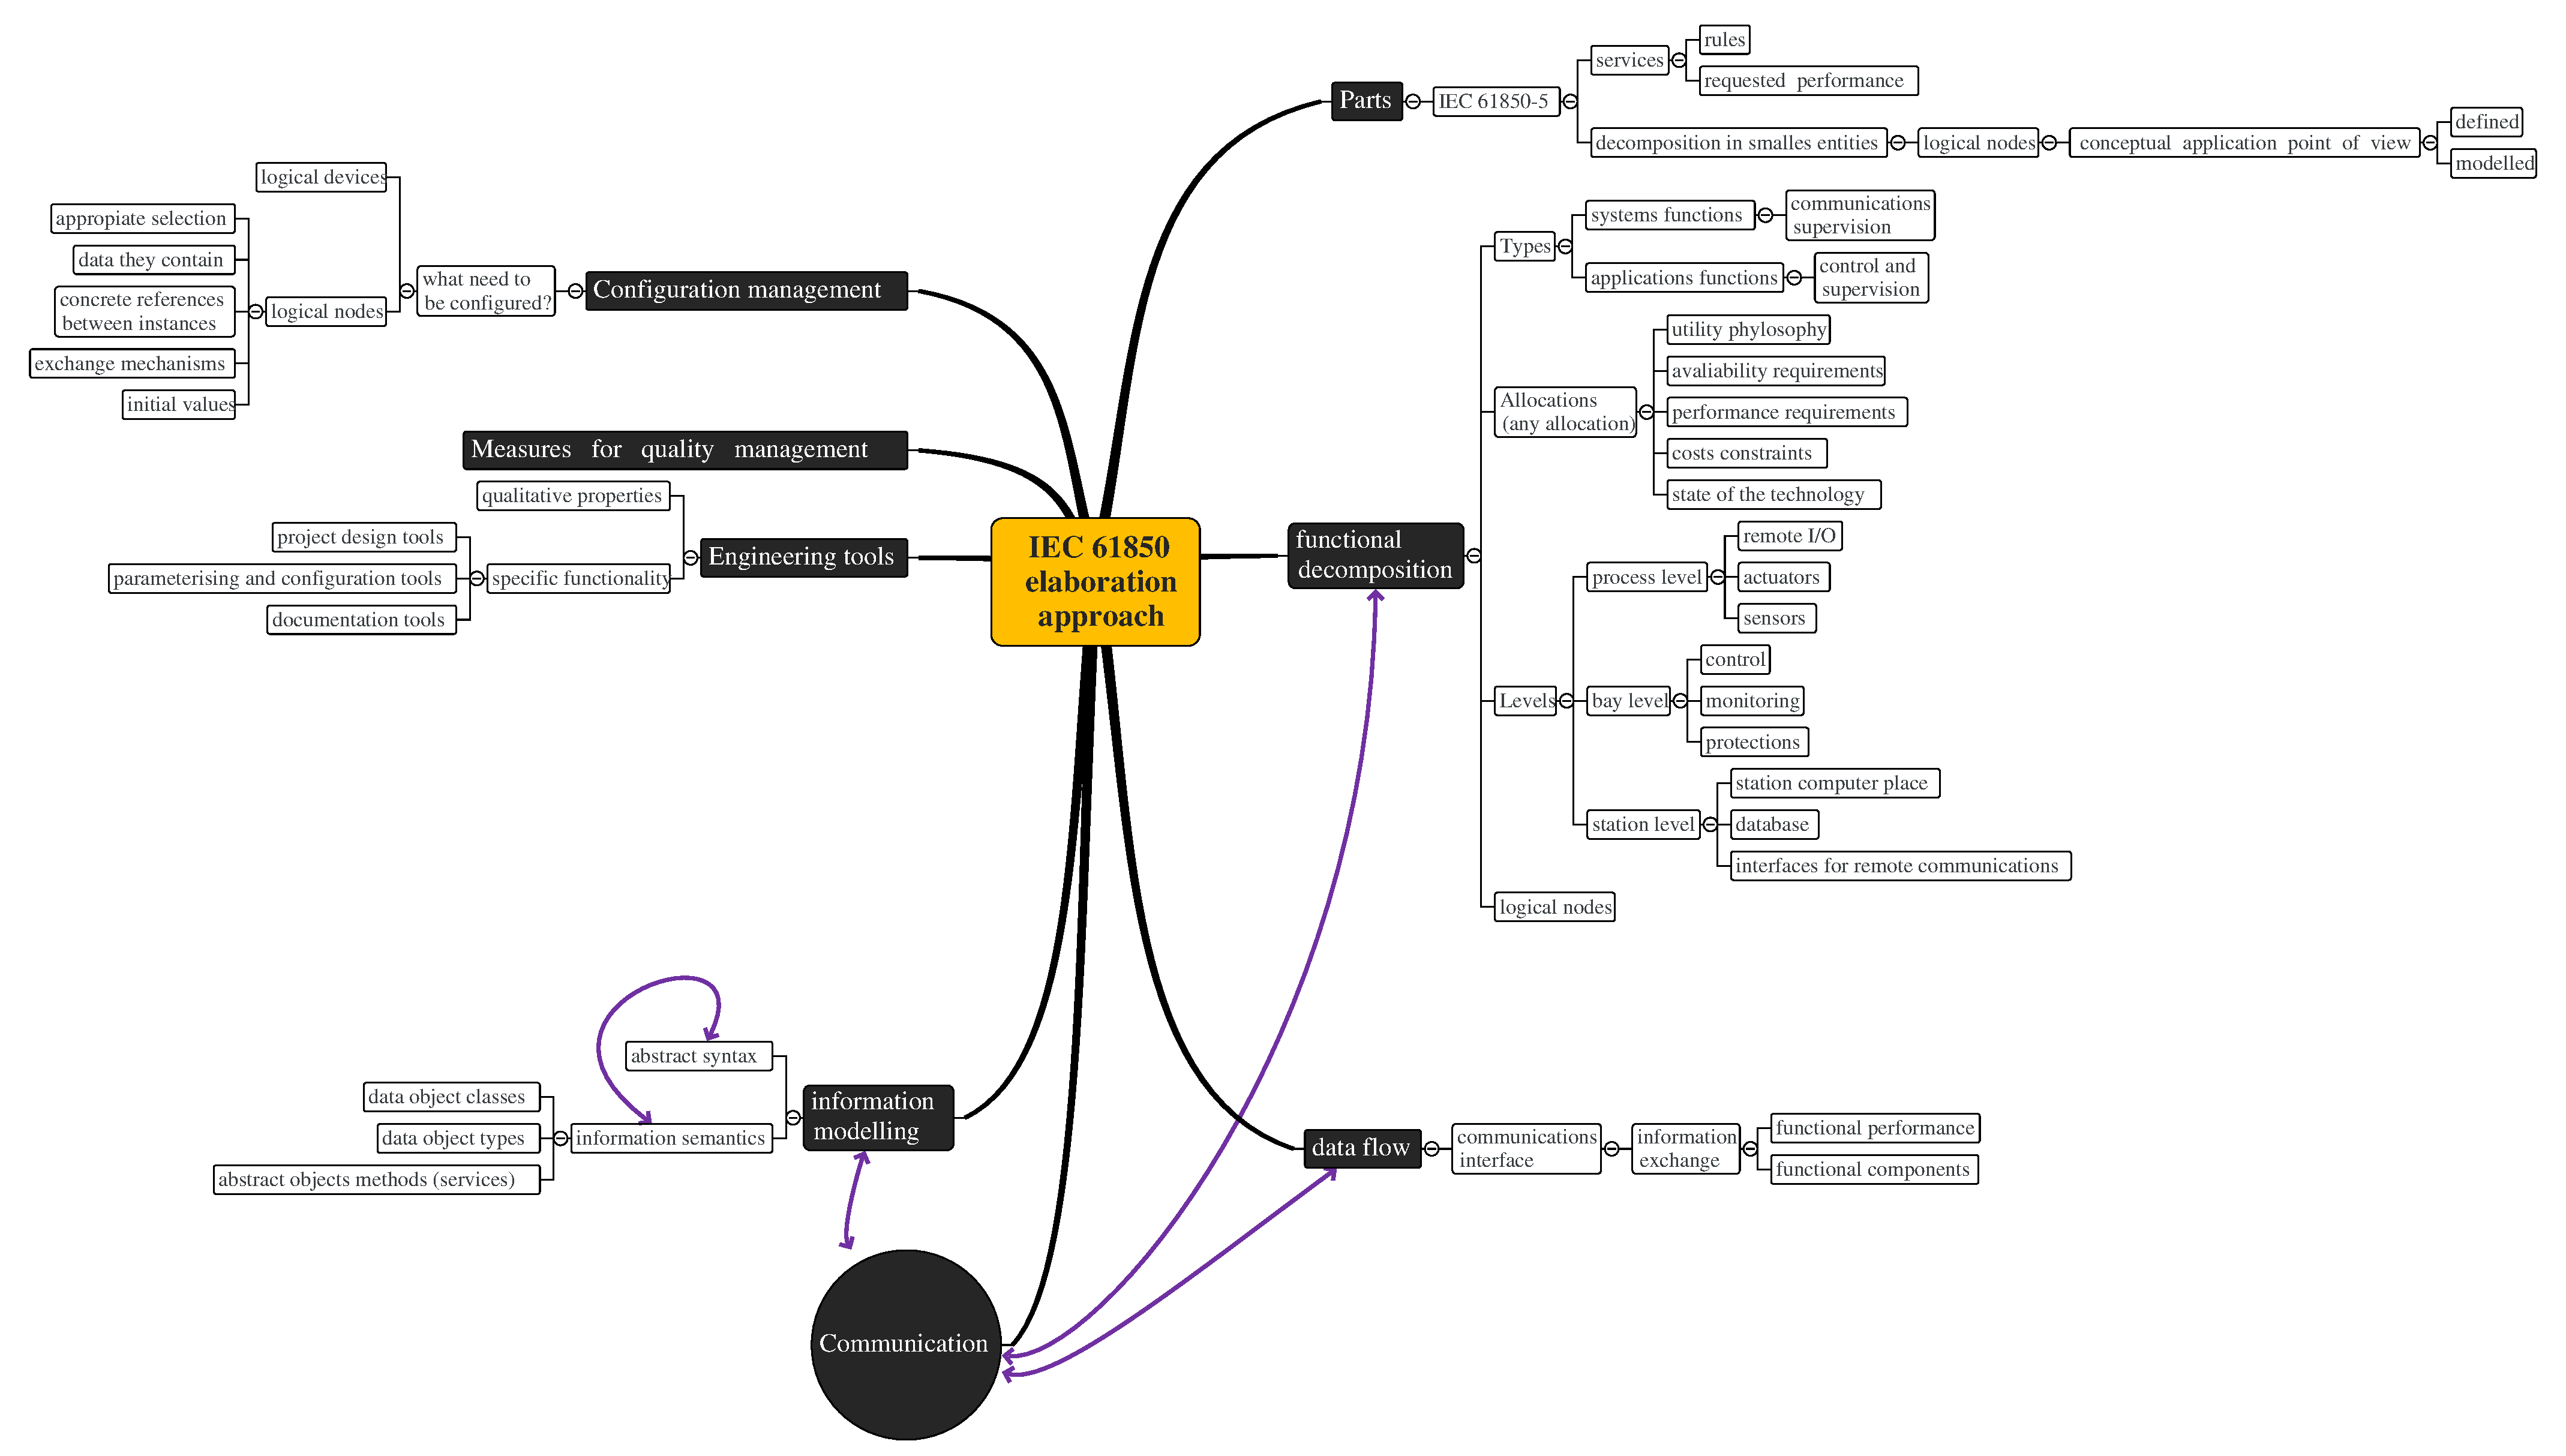
\includegraphics[width=1.0\textwidth]{appendices/IEC61850approach}
%  \caption{Borrador - Esquema del futuro capitulo }
%  \label{fig:lan-networks-topologies-fig3}
%\end{figure}


\section{Objetivos de la norma IEC 61850}

%El objetivo principal de la norma IEC 61850 es la normalizaci�n 
%de la comunicaci�n utilizada en la automatizaci�n de los 
%sistemas el�ctricos de potencia. 

 
El objetivo de la norma IEC 61850 es 
permitir la interoperabilidad entre IEDs
de diferentes fabricantes utilizados en la automatizaci�n de los 
sistemas el�ctricos del sistema el�ctrico. En este caso, 
la interoperabilidad se define como la habilidad de que 
los IEDs operen en la misma red de comunicaci�n compartiendo informaci�n y comandos,
respetando los requisitos funcionales y de desempe�o requeridos, y 
soportando futuros avances tecnol�gicos.

Este objetivo es alcanzado a trav�s de la descomposici�n 
de las interfaces de comunicaci�n en nodos l�gicos
dotados de sintaxis abstractas y sem�nticas 
de la informaci�n a ser intercambiada.
\section{Interoperabilidad}

El requisito m�s importante para la
construcci�n de los grandes sistemas el�ctricos  
acorde a las necesidades actuales es la interoperabilidad en el intercambio de
la informaci�n entre los dispositivos del sistema 
de automatizaci�n de subestaciones.

Gracias a la norma IEC 61850, dos o m�s \Glspl{IED}
del mismo fabricante, o de diferentes fabricantes, tienen
la habilidad de intercambiar informaci�n y utilizar dicha 
informaci�n para la ejecuci�n correcta de funciones espec�ficas
\cite{IEC61850-1:2003}.



\section{Tecnolog�as de comunicaci�n y redes}

La norma IEC 61850 est� dise�ada utilizando especificaciones y normas 
internacionales  de comunicaci�n basadas en Ethernet que permiten la
codificaci�n, decodificaci�n, el transporte y el direccionamiento preciso de la
informaci�n intercambiada entre los equipamientos a trav�s de la red de
comunicaci�n del sistema el�ctrico.      

La figura \ref{fig:pila-protocolos} presenta la pila de protocolos utilizada 
actualmente en la norma IEC 61850.


\begin{figure}
\begin{center}
  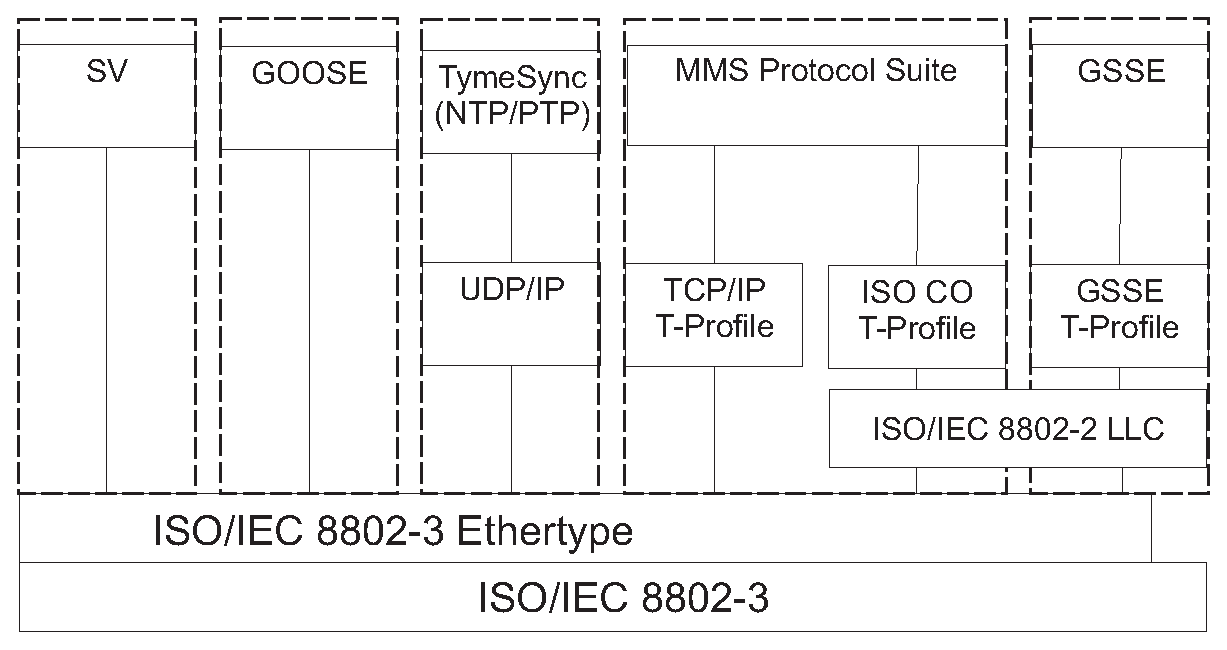
\includegraphics[width=1.0\textwidth]{chapters/introduction/figures/pila-de-protocolos.eps}
  \caption{Pila de protocolos utilizados en la norma IEC 61850}
  \label{fig:pila-protocolos}
\end{center}
\end{figure}

	
\section{Modelo de la informaci�n}
\label{sec:Modelo-informacion-61850}
La norma IEC 61850 define un modelo de informaci�n 
orientado a objetos, y organiza dicho modelo en 
tres niveles: nivel 1, nivel 2 y nivel 3. Este modelo
de informaci�n provee una estructura normalizada
de datos que cubre las necesidades del 
sistema el�ctrico \cite{Ozansoy:2009}. En las figuras
\ref{fig:Intro-LNs} y 
\ref{fig:virtualizacion-LNs} 
se presentan  
el modelo de informaci�n existente en sistemas
de potencia reales, sus equipamientos, 
y la representaci�n virtual del sistema el�ctrico
a trav�s del modelo IEC 61850 que 
responde con el mismo comportamiento que
en el mundo real, pero ejecut�ndose por software.

%\begin{landscape}
\begin{figure}
\begin{center}
  \includegraphics[width=1.0\linewidth]{chapters/introduction/figures/nodos-logicos.eps}
  \caption{Nodos l�gicos}
  \label{fig:Intro-LNs}
\end{center}
\end{figure}
%\end{landscape}

\begin{figure}
\begin{center}
  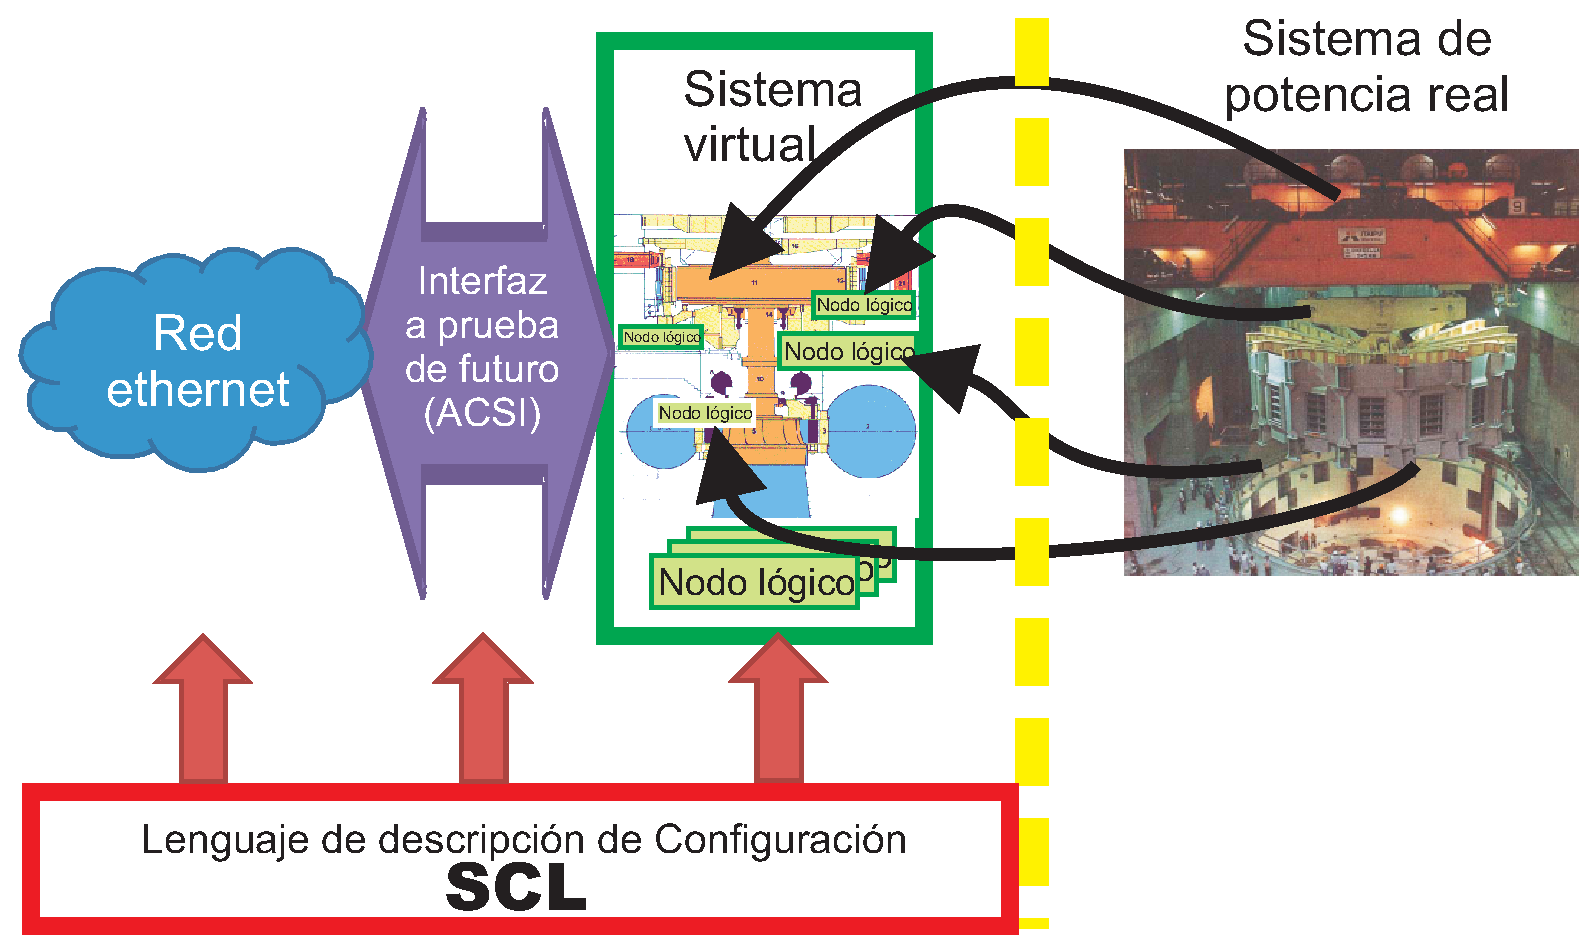
\includegraphics[width=1.0\linewidth]{chapters/introduction/figures/virtualizacion.eps}
  \caption{Virtualizaci�n en el contexto de la norma IEC 61850}
  \label{fig:virtualizacion-LNs}
\end{center}
\end{figure}


	\subsection{Niveles del modelo de la informaci�n}
%	\todo[inline]{agregar algo aca}
	El nivel 1, o \gls{ACSI}, provee las definiciones
	b�sicas de la estructura de la informaci�n, 
	sin vincularlos con ninguna informaci�n del dominio el�ctrico.
	Los niveles 2 y 3 son modelos espec�ficos del dominio el�ctrico 
	utilizados en los objetos de los IEDs. A continuaci�n, se
	describen en forma breve cada uno de estos niveles. 
	
		\subsubsection{Nivel 1: ACSI}
			\label{sec:INTRO-acsi-concepto}
		
		El \gls{ACSI} tiene el rol de sentar las bases
		para un modelo m�s preciso, y a la vez m�s simple de
		la informaci�n.
		%, siendo esta la capa de software
		%que sirve de interfaz con la pila de protocolos utilizados.	
		
		La abstracci�n y el encubrimiento de la informaci�n
		son los pilares fundamentales de todo software 
		orientado a objetos \cite{Levy:1984}. La norma IEC 
		61850-7-2 \cite{IEC61850-7-2:2003} realiza el primer paso
		para la abstracci�n de la informaci�n en base a tecnolog�as 
		orientadas a objetos para proveer  
		una descripci�n simplificada del sistema el�ctrico
		enfatizando algunos detalles o propiedades del sistema,
		y eliminando otros detalles \cite{Shaw:1984}.

		Los pilares del \textbf{ACSI} son: 
		      \begin{itemize}
		        \item El modelo de informaci�n abstracto: Las clases
		        abstractas que definen la estructura 
		        de toda la informaci�n.
		        \item El modelo de servicios abstractos: 
				Las interfaces abstractas definidas en el 
				apartado IEC 61850--7--2 \cite{IEC61850-7-2:2003}
				declaran un grupo de m�todos de clase que permiten
				a los \Glspl{IED} comunicar las instancias de la clase 
				con otras instancias.
				Los servicios abstractos definidos en el \gls{ACSI} 
				sirven al proyectista para 
				conocer los siguientes aspectos de los 
				servicios de comunicaci�n: 
				su comportamiento, 
				sus entradas, salidas, y opcionalmente 
				el tratamiento de los errores si fuere el caso,
				pero sin la necesidad de conocer como 
				ese comportamiento est� implementado
				en el \gls{IED} (el fabricante de \Glspl{IED} es 
				el responsable del mapeo de los servicios
				\gls{ACSI} a la pila de protocolos 
				seleccionados por la norma IEC 61850).
		      \end{itemize}
			
		\subsubsection{Nivel 2: Clases de Datos Comunes o \textbf{CDC}}
			En el apartado IEC 61850--7--3 \cite{IEC61850-7-3:2003}
			los \Glspl{CDC} extienden las clases abstractas 
			que se emplearon para crear la estructura b�sica 
			del modelo de informaci�n definido en el
			\gls{ACSI}.
			
		\subsubsection{Nivel 3: Nodos L�gicos y Clases de Datos compatibles}
			Este nivel del modelo de la informaci�n est� definido
			en el apartado IEC 61850--7--4, y ya es utilizado 
			para situaciones espec�ficas en el contexto el�ctrico 
			(en t�rminos de dise�o \gls{O-O-es} ser�an
			las definiciones de las clases finales).
			Los modelos del nivel 3 son definidos como
			\emph{modelos de objetos compatibles} seg�n 
			la IEC 61850,
			a trav�s de tipos de nodos l�gicos compatibles
			y tipos de datos compatibles (por ejemplo, posici�n del 
			interruptor con estampa de tiempo de calidad del dato).
			Son estas definiciones las que proveen la sem�ntica
			al modelado de la informaci�n de los sistemas el�ctricos
			realizada en la norma IEC 61850.  





\section{Funciones del Sistema de Automatizaci�n de Subestaciones}

Las funciones del \gls{SAS} son las tareas que 
tienen que ser realizadas
dentro de la hidroel�ctrica.

En las centrales hidroel�ctricas existen funciones 
para monitorear, controlar y proteger 
los equipamientos del sistema. Tambi�n 
existen funciones para la configuraci�n del sistema,
gerenciamiento de la comunicaci�n,
o gerenciamiento del software. \cite{IEC61850-5:2003}.



\subsection{Libre ubicaci�n de funciones}

	Desde hace m�s de 20 a�os han 
	surgido las necesidades (y se comenz� a investigar al respecto)
	de tener la libertad de distribuir efectivamente
	en diferentes equipamientos 
	los objetos (virtuales) que realizan 
	tareas computacionales.
	
	Estas frases fueron extraidas de la investigaci�n
	de Jazayeri, de 1988 \cite{Jazayeri:1988}:


%	The effective distribution of Logical Nodes 
%	on diferents IEDs  
%	is a reality thanks to researches about 
%	the structure of distributed systems. More 
%	than 20 years ago emerged requirements 
%	for the object paradigm to suport the 
%	design and development of distributed systems.
	
%	Theses quotes were extracted from Jazayeri 
%	1988 research:
	
	\emph{
	``An object on one node can send a (multicast) message 
	to several other objects \ldots''
	} \cite{Jazayeri:1988} (Hoy en d�a esto es una realidad a trav�s de 
	las asociaciones \textbf{MCAA} y los mensajes \textbf{GSE}
	definidos en las clases \textbf{ACSI})
	
	\emph{
	`` \ldots The ability to group 
	a set of objects and address them as one entity 
	is important in many applications both from an 
	efficiency point of view and from a program 
	structuring point of view \ldots'' 
	} \cite{Jazayeri:1988} (este aspecto tambi�n 
	es una realidad, en la norma 
	IEC 61850 se utilizan \textbf{DATA--SETs} \cite{Ozansoy:2009b}, 
	\textbf{FCD},
	\textbf{FCDA}, entre otros).
	
	\emph{
	`` \ldots a final 
	difference is that our objects are active and 
	not reactive, in the sense that they can start 
	up spontaneosly performing operations, not 
	necessarily only in response to method invocations.
	Such a facility is useful, for example, to allow objects 
	to monitor the enviroment and change their behavior based 
	on changes in the enviroment \ldots'' 
	} \cite{Jazayeri:1988} (En el contexto de la norma IEC 61850
	los objetos activos ser�an las clases abstractas
	(utilizadas como interfaz para el env�o de los mensajes)
	\textbf{URCB}, \textbf{BRCB}  a trav�z de 
	sus opciones de \textbf{trigger}) \cite{Jazayeri:1988}.
	 
%	Some active objects 
%	are GOOSE, URCB and some passive object 
%	are \todo{completar y ver si esta bien})
	
	
	
	Las especificaciones de la norma IEC 61850,
	basadas en
	tecnolog�as orientadas a objetos ya maduras,
	consiguen atender 
	los requisitos de disponibilidad,
	la filosof�a de la central hidroel�ctrica,
	requisitos de performance,
	costos,
	y el estado del arte de la tecnolog�a. 
	
	
\subsection{Clasificaci�n de las funciones seg�n los niveles}
	Seg�n los niveles en el cual el IED se desempe�a,
	sus funciones pueden ser clasificadas en 3 grupos: 
	
	\begin{itemize}
	  \item Nivel de proceso: I/O remotas, actuadores, sensores.
	  \item Nivel de bay: IEDs de control, monitoreo y protecci�n
	  \item Nivel de estaci�n: Estaci�n de ingenier�a de la subestaci�n,
	  base de datos, interfaces para comunicaci�n remota.  
	\end{itemize}
	
	

%\section{Virtualizaci�n}


\section{Lenguaje de descripci�n de Configuraci�n de Subestaciones -- SCL}

%El proceso de ingenier�a IEC 61850 de todo el sistema de automatizaci�n de
%subestaciones el�ctricas se realiza utilizando el Lenguaje de Configuraci�n de
%Subestaciones.     

El \gls{SCL} tiene como objetivo describir la
estructura de los equipamientos primarios del sistema
de potencia, el sistema de comunicaci�n y la comunicaci�n
a nivel de aplicaci�n.

A nivel de aplicaci�n, el \gls{SCL} permite describir 
c�mo los \textbf{Data Objects} est�n agrupados para
su env�o, c�mo el \gls{IED} despacha el intercambio de 
la informaci�n (\textbf{Trigger}), cu�les servicios 
se eligieron durante el dise�o del sistema,
qu� datos de entrada de otros IEDs son necesitados,
qu� dispositivos l�gicos 
est�n configurados en cada \gls{IED}, sus nodos l�gicos con
sus respectivas plantillas e instancias.

A continuaci�n, se enumeran los principales
usos del \gls{SCL}.
\begin{itemize}
	\item Definici�n de la estructura del modelo de la informaci�n del sistema.
	\item Descripci�n del sistema a trav�s de nodos l�gicos. 
	\item V�nculo de los nodos l�gicos del sistema con los nodos l�gicos de los
	IEDs.
	\item Creaci�n de las conexiones l�gicas.
	\item Definici�n de los m�todos de intercambio de la informaci�n.
	\item Configuraci�n de los par�metros de la red.
	\item Documentaci�n formal del proceso de ingenier�a.
\end{itemize}

%\begin{figure}
%  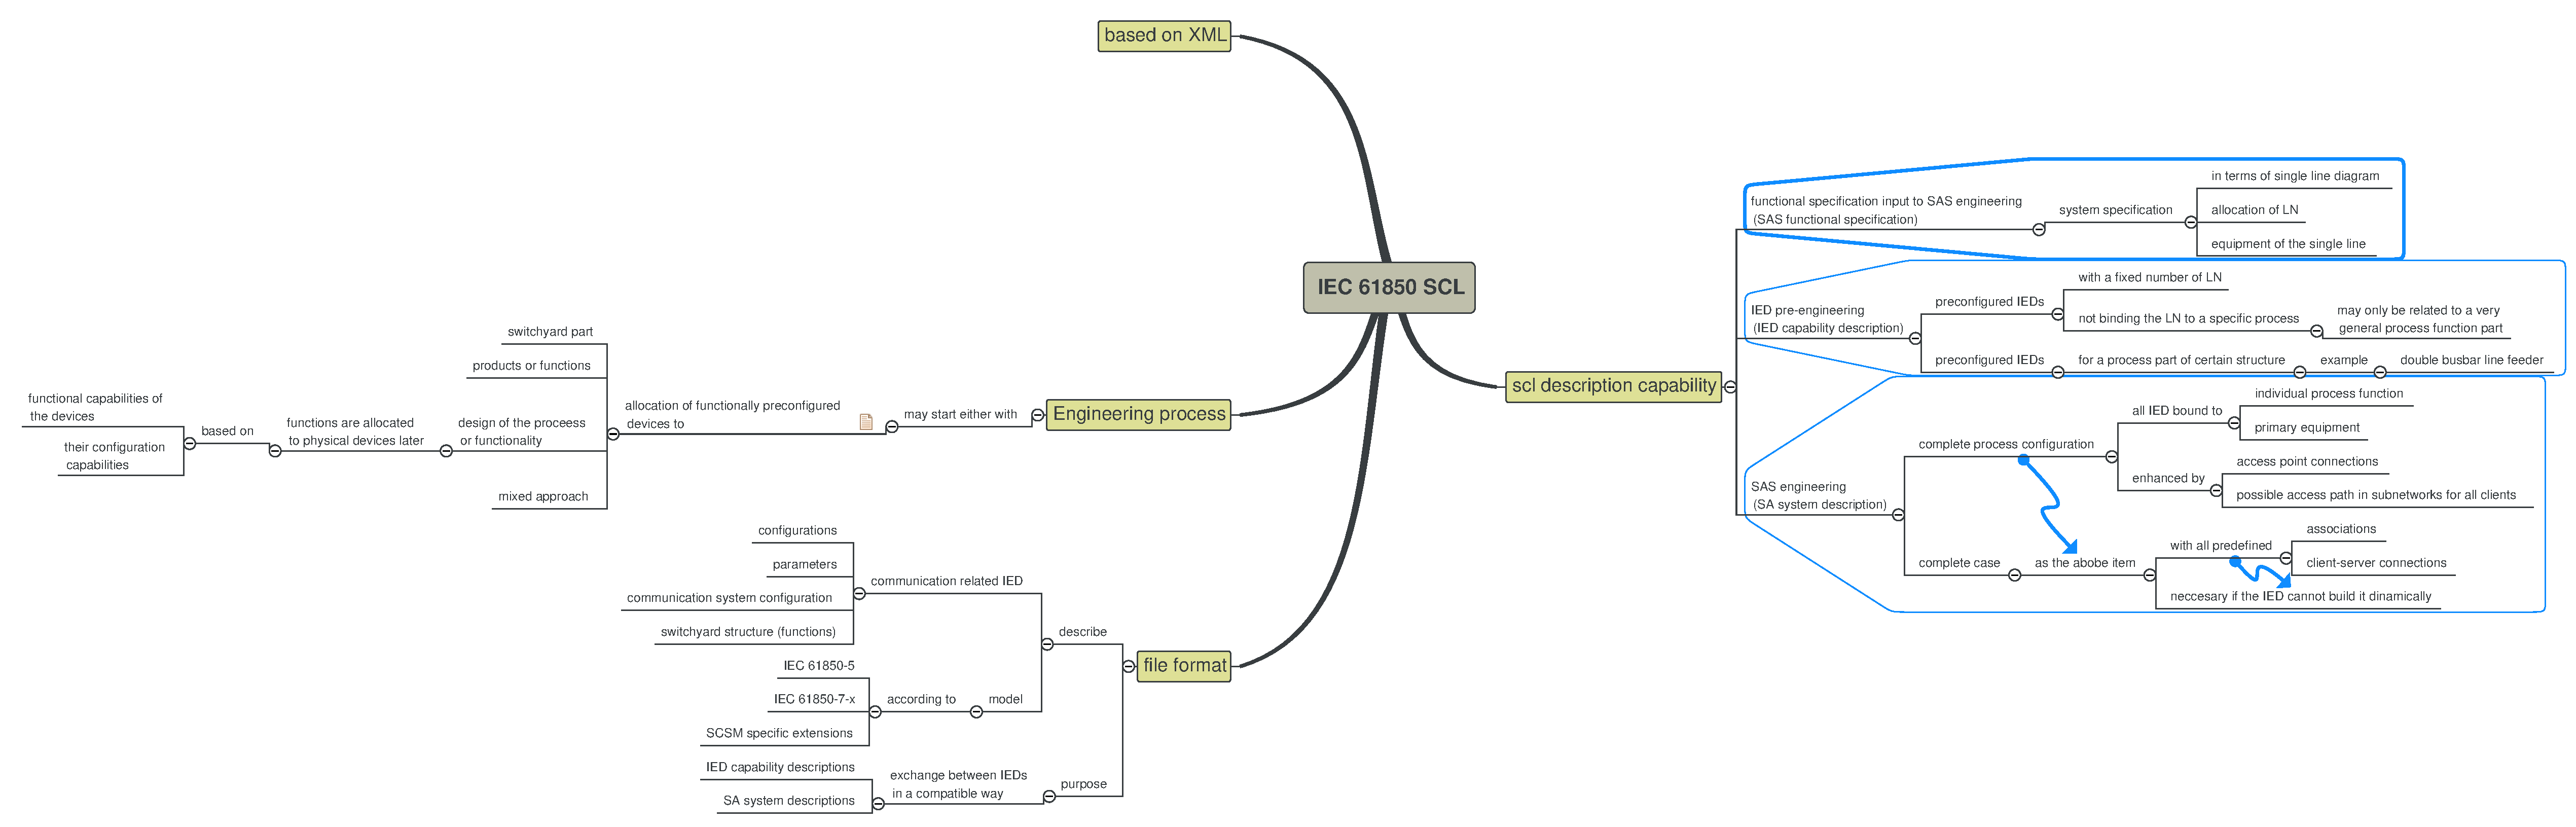
\includegraphics[width=1.0\textwidth]{appendices/IEC61850SCL}
%  \caption{Borrador - Esquema del futuro capitulo }
%  \label{fig:lan-networks-topologies-fig4}
%\end{figure}

\subsection{Variantes SCL}

Los archivos \gls{SCL}, dependiendo de su contenido, 
seg�n la IEC 61850--6 (Edici�n 1) \cite{IEC61850-6:2004} 
se clasifican en:

\begin{itemize}
  \item SSD: La variante SSD (\emph{System Specification Description}) 
  contiene el diagrama unifilar de la subestaci�n (a trav�s de los elementos
  \textbf{Header}, \textbf{Substation} y opcionalmente el elemento
  \textbf{DataTypeTemplates}).
  \item ICD: La variante ICD (\emph{IED Capability Description}) 
  describe las capacidades de los IEDs (IEDs a�n no configurados)
  (A trav�s de los elementos \textbf{IED}, \textbf{Communication},
  \textbf{Header} y \textbf{DataTypeTemplates}).
  \item CID: La variante CID (\emph{Configured IED Description}) 
  es la descripci�n de configuraci�n
  de un IED. Incluye todas las configuraciones IEC 61850 
  que puedan ser configurables: asociaciones, parametrizaciones
  de la red, entre otros.   (A trav�s de los elementos \textbf{IED}, 
  \textbf{Communication}, \textbf{Header} y \textbf{DataTypeTemplates}).
  A diferencia de la variante ICD, un CID tambi�n contiene 
  datos de los dem�s IEDs con los cuales se comunica.
  \item SCD: La variante SCD (\emph{Substation Configuration Description}) 
  contiene los archivos CID y su 
  relaci�n con respecto a la estructura del sistema el�ctrico
  descripto en el SSD, que tambi�n est� incluido en el SCD.
  (Contiene todos los elementos SCL, que pueden ser observados en 
  la figura \ref{fig:SCL-main-parts}.  
\end{itemize}
 
\section{Herramientas de ingenier�a}

Como apoyo fundamental para la ejecuci�n de estas tareas, la norma IEC 61850
contempla y define las llamadas herramientas de ingenier�a, que son programas
altamente especializados concebidos para elaborar los archivos necesarios para
especificar y configurar el sistema de automatizaci�n de una subestaci�n
el�ctrica que incorpore a la norma IEC 61850 como patr�n de comunicaciones [2].
Estas herramientas deber�an ofrecer una amplia gama de funcionalidades, como,
por ejemplo, la posibilidad de configurar dispositivos de marcas diferentes que
integren un mismo sistema, con base en las caracter�sticas de interoperabilidad
perseguidas por la norma \cite{PTI:SESEP2010}.


De acuerdo a esta norma, las herramientas de ingenier�a necesarias para los
proyectos realizados en conformidad con la misma deben posibilitar la creaci�n
y documentaci�n de los procesos de ingenier�a, tales como: gerenciamiento del
proyecto, parametrizaci�n de dispositivos y documentaci�n del sistema de
automatizaci�n de subestaciones por medio de la utilizaci�n del \gls{SCL}.         


\section{Partes de la norma IEC 61850}

La norma IEC 61850 consta de varias 
partes. En cada una de ellas se trata 
un aspecto espec�fico sobre 
las redes y sistemas de comunicaci�n 
de subestaciones, y por extensi�n, 
de hidroel�ctricas.  
A continuaci�n, se citan las 
partes de la norma IEC 61850 
y su estado de publicaci�n
en la fecha de realizaci�n de este trabajo:

\begin{itemize}
  \item IEC 61850--1:2003 	\cite{IEC61850-1:2003}:
	Introduction and overview (TR Ed1:2003--04).


  \item IEC 61850--2:2003		\cite{IEC61850-2:2003}: 
	Glossary (TS Ed1:2003--08).

	
  \item IEC 61850--3:2002		\cite{IEC61850-3:2002}:  
	General requirements(IS Ed1:2002--02).
  
  
  \item IEC 61850--4:2002		\cite{IEC61850-4:2002}: 
	System and project management  (IS Ed1:2002--01).
  
  
  \item IEC 61850--5:2003		\cite{IEC61850-5:2003}:  
	Communication requirements for 
	functions and device models  (IS Ed1:2003--07).
  
  
  \item IEC 61850--6:2004		\cite{IEC61850-6:2004}:   
	Configuration description language
	for communication in electrical
	substations related to IEDs  (IS Ed1:2004--03).
  
  
  \item IEC 61850--7--1:2003	\cite{IEC61850-7-1:2003}:  
	Basic communication structure -- Principles and models  (IS Ed1:2003--07).
  
  
  \item IEC 61850--7--2:2003	\cite{IEC61850-7-2:2003}:  
	Basic communication structure -- 
	Abstract communication service interface (ACSI)  (IS Ed1:2003--05).
	  
  
  \item IEC 61850--7--3:2003	\cite{IEC61850-7-3:2003}:  
	Basic communication structure -- Common data classes  (IS Ed1:2003--05).
  
  
  \item IEC 61850--7--4:2003	\cite{IEC61850-7-4:2003}:  
	Basic communication structure -- 
	Compatible logical node classes and data classes  (IS Ed1:2003--05).
  
  
  \item IEC 61850--7--410:2007	\cite{IEC61850-7-410:2007}:  
	Hydroelectric power plants -- 
	Communication for monitoring and control  (IS Ed1:2007--08).
  
  
  \item IEC 61850--7--420:2009	\cite{IEC61850-7-420:2009}:  
	Communications systems for distributed 
	energy resources (DER) -- Logical nodes  (IS Ed1:2009--03).
  
  
  \item IEC 61850--7--430 \cite{IEC61850-7-430:200-X}:  
	Communication system for distribution 
	feeder and network equipment  (57/954/NP).
  
  
  \item IEC 61850--7--5:2010	\cite{IEC61850-7-5:2010}:  
Basic communication structure --� 
Usage of information models for substation
automation applications  (DC 2010-08).
  
  
  \item IEC 61850--7--500:2010	\cite{IEC61850-7-500:2010}:  
	Use of logical nodes to model functions 
	of a substation automation system  (DC 2010--08).
  
  
  \item IEC 61850--7--510:2009	\cite{IEC61850-7-510:2009}:  
	Use of logical nodes to model 
	functions of a hydro power plant  (DC 2009--12).
  
  
  \item IEC 61850--7--520:2010	\cite{IEC61850-7-520:2010}:  
	Use of logical nodes to model functions 
	of distributed energy resources  (Draft 2010).
  
  
  \item IEC 61850--7--10:2009	\cite{IEC61850-7-10:2009}: 
	Web--based and structured access to the 
	IEC 61850 information models  (DC 2009--12).
  
  
  \item IEC 61850--8--1:2004	\cite{IEC61850-8-1:2004}: 
	Specific communication service 
	mapping (SCSM) -- 
	Mappings to MMS (ISO/IEC 9506--1 and 
	ISO/IEC 9506--2) and to ISO/IEC 8802--3  (IS Ed1:2004--05).
	  
  
  \item IEC 61850--9--1:2003	\cite{IEC61850-9-1:2003}:
	Specific communication service mapping (SCSM) -- 
	Sampled values over serial unidirectional
	multidrop point to point link  (IS Ed1:2003--05).
  
  
  \item IEC 61850--9--2:2004	\cite{IEC61850-9-2:2004}:
	Specific communication service mapping (SCSM) -- 
	Sampled values over ISO/IEC 8802--3  (IS Ed1:2004--04).

  
  \item IEC 61850--80--1 \cite{IEC61850-80-1:200-XXXXXX}:
	Guideline to exchanging information from a 
	CDC--based data model using IEC 60870--5--101 or IEC
	60870--5--104  (TS Ed1:2008--12).
  
  
  \item IEC 61850--90--1 \cite{IEC61850-90-1:200-XXXXXX}:
	Using IEC 61850 for the communication 
	between substations  (TS Ed1:2009--08).
  
  
  \item IEC 61850--90--2 \cite{IEC61850-90-2:200-XXXXXX}:
	Using IEC 61850 for the communication 
	between substations and control centres  (Draft 2010--01).
  
  
  \item IEC 61850--90--3 \cite{IEC61850-90-3:200-XXXXXX}:
	Using IEC 61850 for Condition Monitoring  (Draft 2010--06).
  
  
  \item IEC 61850--90--4 \cite{IEC61850-90-4:200-XXXXXX}:
	Network Engineering Guidelines  (Draft 2010--04).
  
  
  \item IEC 61850--90--5 \cite{IEC61850-90-5:200-XXXXXX}:
	Using IEC 61850 to transmit 
	synchrophasor information according to IEEE C37.118  (Draft 2010--06).
  
  
\end{itemize}
 
 
Cada parte de la norma est� compuesta por cl�usulas 
(en los Tissues \cite{IEC61850:tissues} se utiliza este nombre para las
secciones de cada parte de la norma), y nuevamente, 
cada cl�usula posee uno o m�s p�rrafos. En este trabajo,
al realizar las citaciones de esta norma, el autor 
referencia las cla�sulas (en caso que sea necesario) de la siguiente 
forma: \cite[cl. 1]{IEC61850-1:2003}.


\section{Partes de la norma IEC 61850 utilizadas para modelar la informaci�n de centrales hidro--el�ctricas}

De entre las partes mencionadas en la secci�n anterior destacamos las m�s importantes para este trabajo de modelado de la informaci�n 
del sistema de regulaci�n de una unidad generadora t�pica de Itaipu:

\begin{itemize}
  \item IEC 61850--7--4:2003	\cite{IEC61850-7-4:2003}:  
	Basic communication structure -- 
	Compatible logical node classes and data classes  (IS Ed1:2003--05).
  \item IEC 61850--7--410:2007	\cite{IEC61850-7-410:2007}:  
	Hydroelectric power plants -- 
	Communication for monitoring and control  (IS Ed1:2007--08).
\end{itemize}

La parte 7--4--10 define formalmente los nodos l�gicos para centrales hidroel�ctricas, mientras que la parte 7--4 
define los nodos l�gicos m�s generales, utilizados tanto en hidroel�ctricas, subestaciones, u otra �rea del sistema el�ctrico. 

Este apartado tiene relaci�n con la utilizaci�n de los nodos l�gicos en hidroel�ctricas, pero 
durante la realizaci�n de este trabajo este documento a�n se encontraba en proceso de redacci�n, 
y el autor de este trabajo no ha tenido acceso al borrador.
\begin{itemize}
  \item  IEC 61850--7--510:2009	\cite{IEC61850-7-510:2009}:  
	Use of logical nodes to model 
	functions of a hydro power plant  (DC 2009--12).
\end{itemize}


\section{Descripci�n del regulador de velocidad actual de una unidad generadora t�pica de Itaipu}

Los generadores hidroel�ctricos de la Itaipu est�n interconectados a los sistemas el�ctricos del Paraguay y del Brasil. Uno 
de los requisitos m�s importantes para dicha interconexi�n es que los generadores deben estar sincronizados a la frecuencia 
del sistema. Para ello, los sistemas de regulaci�n de velocidad abren o cierran las paletas del distribuidor de la turbina para controlar su rotaci�n  
en funci�n a la carga, controlando asi la variaci�n de frecuencia hasta l�mites permitidos. El regulador de velocidad tambi�n 
controla la velocidad de rotaci�n sin carga de la unidad durante la fase de puesta en marcha, 
permitiendo una r�pida sincronizaci�n con el sistema. El papel del regulador puede extenderse 
a su participaci�n en la regulaci�n secundaria de un esquema de intercambio de cargas de potencia/frecuencia entre �reas.

Estos regualadores de velocidad se clasifican como reguladores electro-hidr�ulicos 
anal�gicos del tipo acelero-tacom�trico con estatismo y constan de circuitos hidr�ulicos encargados 
de mover las paletas del distribuidor (tanques, v�lvulas, servomotores), 
circuitos neum�ticos que acumulan energ�a potencial en forma de aire comprimido que poseen un 
transductor electro-hidr�ulico que sirve como interfaz de comando
y de circuitos electr�nicos que controlan el desv�o y la rapidez de variaci�n de la velocidad de rotaci�n de la unidad generadora 
a trav�s de una acci�n proporcional, integral y derivativa (PID). 

El documento \cite{Itaipu:195860C8841ER0} describe la estructura del regulador de velocidad de la siguiente manera:
\emph{``El regulador de velocidad `Rapid 77' posee una
estructura en dos niveles jer�rquicos, en la cual el sector
de la regulaci�n de velocidad y de carga se halla f�sica y
funcionalmente separado del sector de posicionamiento.
La realimentaci�n para el PID es tomada desde la se�al
el�ctrica suministrada a la v�lvula principal de distribuci�n
del aceite, y el circuito hidr�ulico de los servomotores,
que sirve para posicionar los �labes del distribuidor,
posee sus propios medios de realimentaci�n por v�a de
una se�al tomada de los transductores ubicados sobre
el mecanismo de operaci�n de los �labes y sobre el
husillo de la v�lvula principal de distribuci�n, v�ase la
figura \ref{fig:estructura-rv-rapid77}. Esta estructura en dos niveles facilita la
configuraci�n del regulador de velocidad, asiste al
mantenimiento y mejora la confiabilidad operacional.''}
La tabla \ref{table:esquema-funcional-rv} describe este esquema de la figura \ref{fig:estructura-rv-rapid77}.

\begin{figure}
\begin{center}
  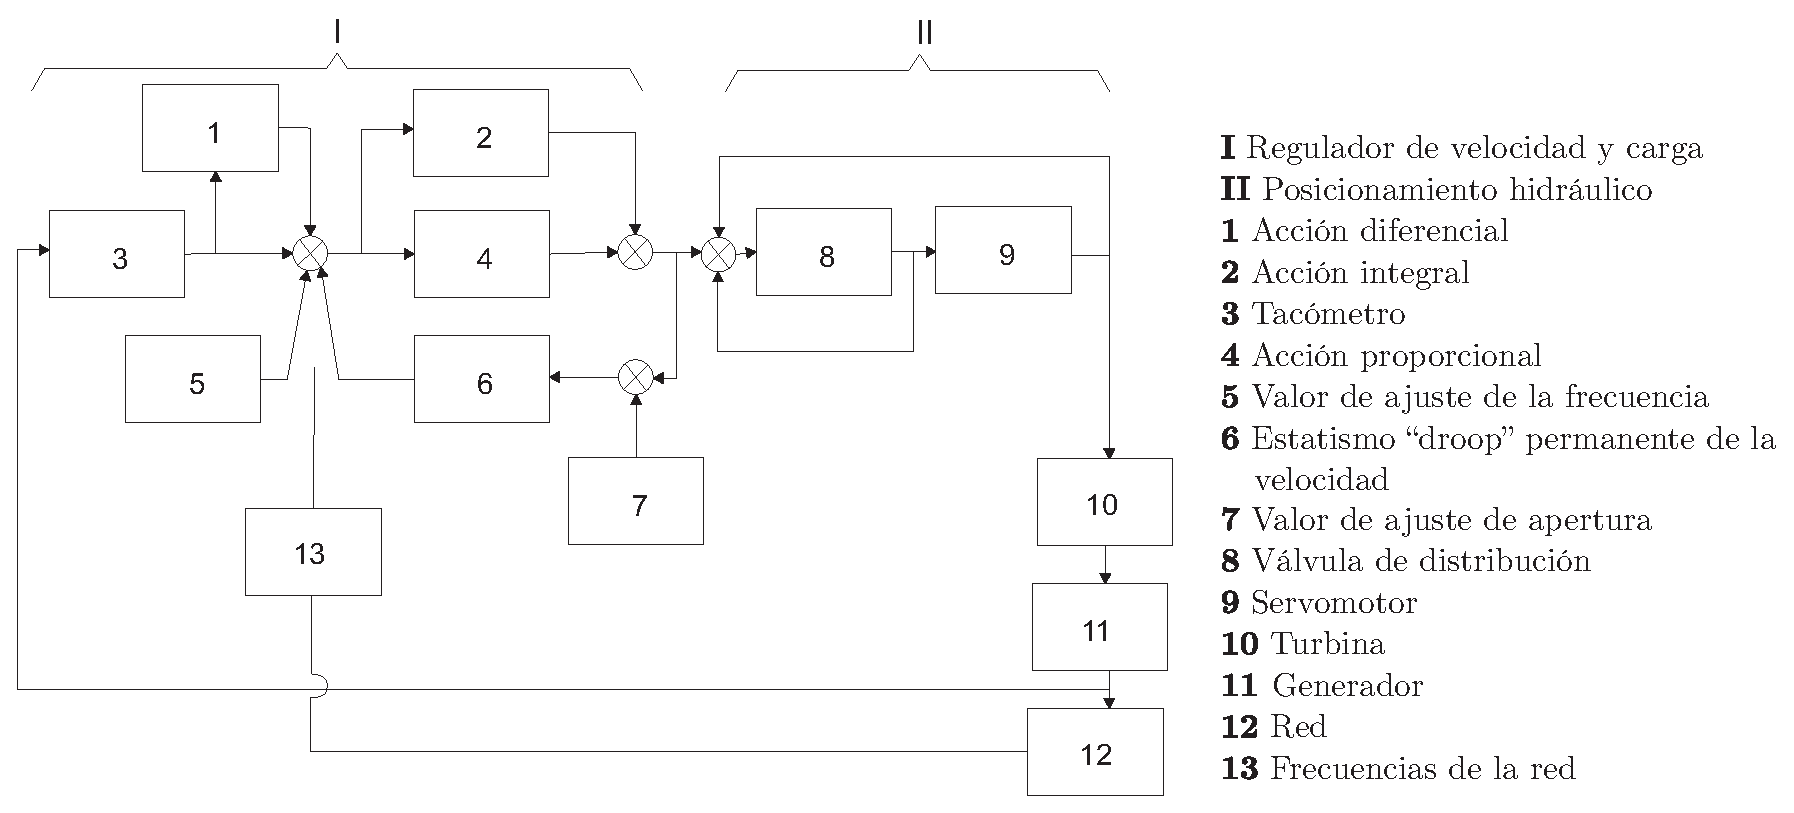
\includegraphics[width=1.0\linewidth]{chapters/introduction/figures/estructura-rv-rapid77.eps}
  \caption{Estructura funcional del regulador Rapid 77}
  \label{fig:estructura-rv-rapid77}
\end{center}
\end{figure}


\subsection{Caracter�sticas b�sicas}

El sistema de regulaci�n actual est� constituido por tres circuitos: El circuito hidr�ulico, el circuito de aire comprimido,
y el circuito regulador electr�nico, cuyo esquema funcional es indicado en la figura \ref{fig:esquema-funcional-rv-rapid77}.

\subsubsection{El circuito regulador electr�nico}
B�sicamente, est� compuesto de:
\begin{itemize}
	\item Circuitos sensibles a la frecuencia del grupo
	\item Dispositivos de regulaci�n de carga -- frecuencia y retroalimentaciones de potencia y de apertura.
	\item Mezclador general y amplificador de potencia.
	\item Limitador de apertura o de potencia.
	\item Circuito posicionador y amplificador de potencia.
	\item Circuito taquim�trico auxiliar.
\end{itemize}

\subsubsection{El circuito hidr�ulico}
El principio de funcionamiento y su conjunci�n con el circuito el�ctrico se encuetra esquem�ticamente descripto en 
la figura \ref{fig:cadena-hidraulica-del-rv}. Sus componentes b�sicos son:


\begin{itemize}
	\item Transductor electro -- hidr�ulico (Actuador)
	\item V�lvula distribuidora
	\item Servomotor
	\item Tanques de aire/aceite
	\item Bombas de aceite
	\item V�lvula de aislamiento
	\item Sistema de amortiguamiento
	\item Sobrevelocidad hidromec�nica
	\item Tanque de aceite (tanque sin presi�n)
\end{itemize}


\subsubsection{El sistema de aire comprimido}
\begin{itemize}
	\item Grupo moto--compresores de alta presi�n (3 etapas).
	\item Tanque de aire comprimido
	\item Eletrov�lvula BE
\end{itemize}

\begin{figure}
\begin{center}
  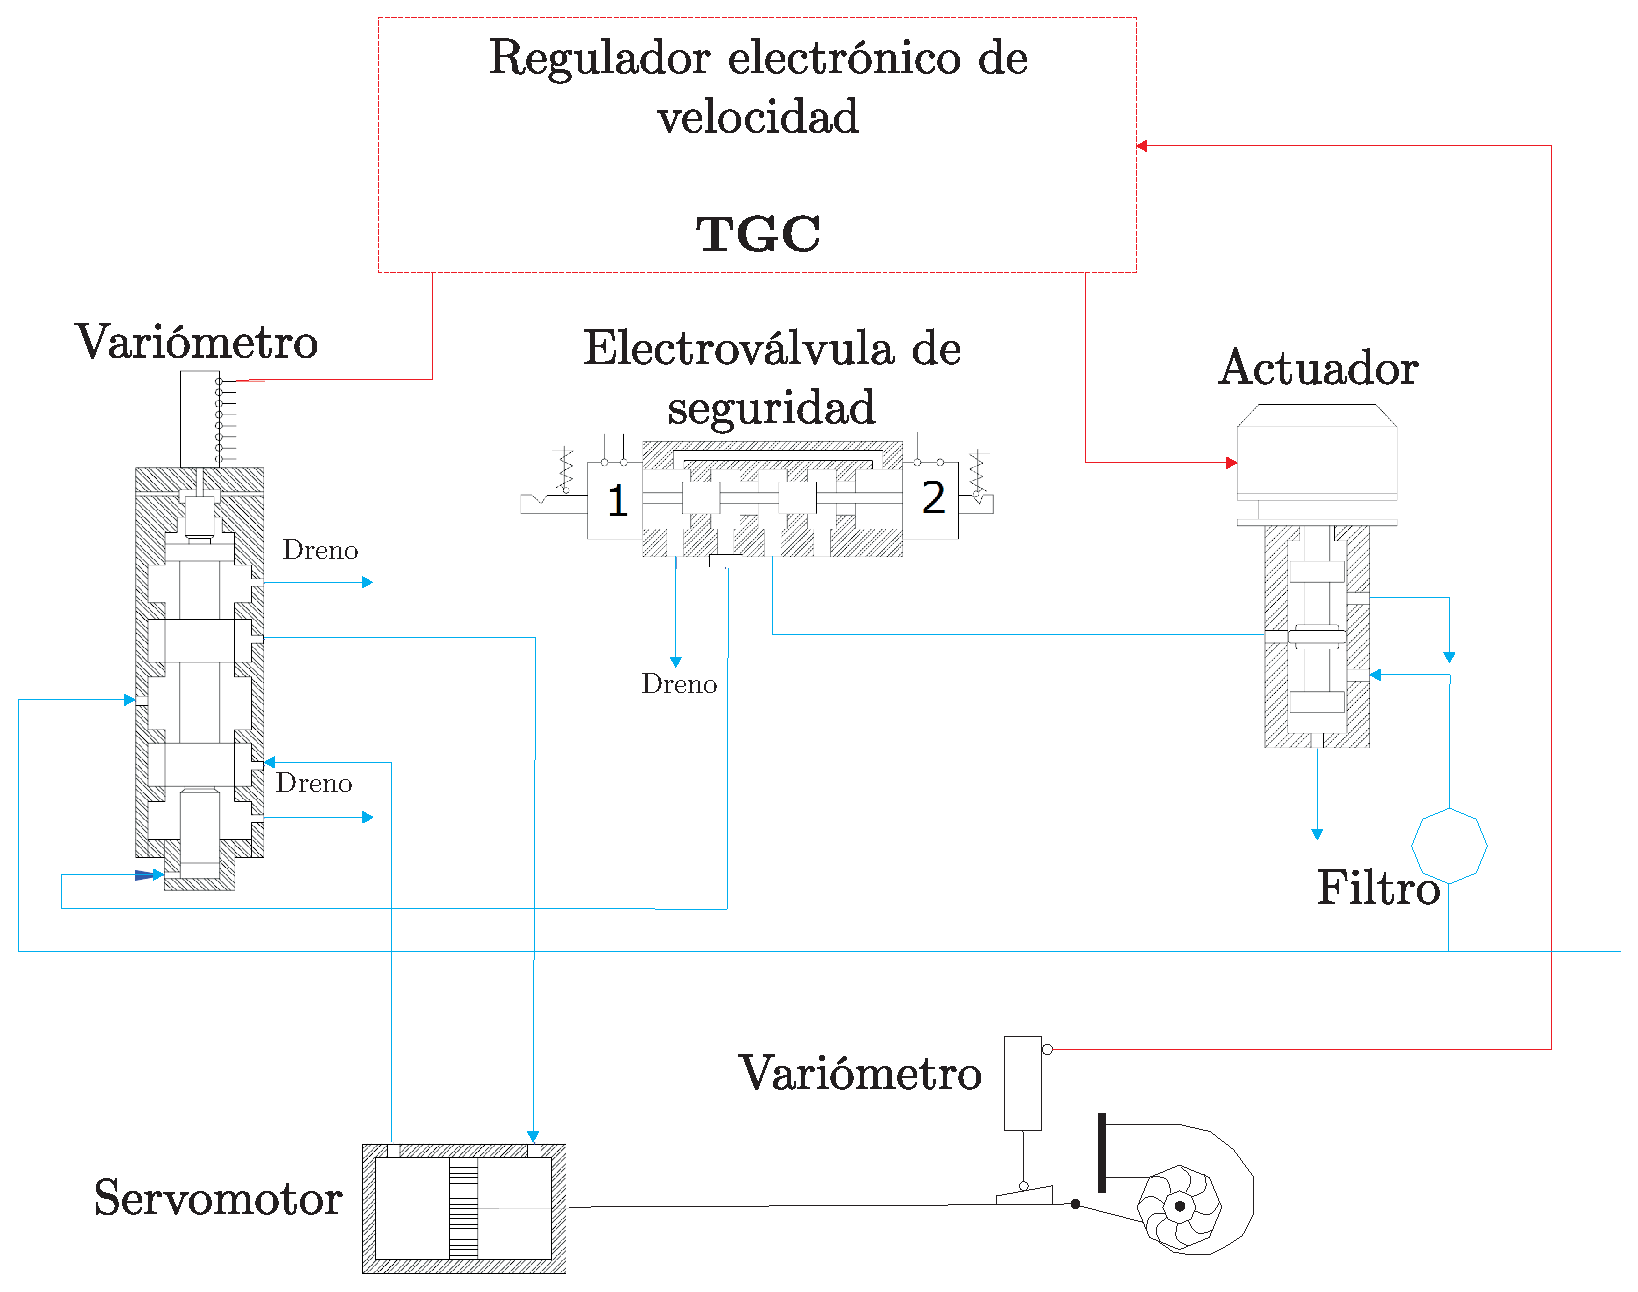
\includegraphics[width=1.0\linewidth]{chapters/introduction/figures/cadena-hidraulica-del-rv.eps}
  \caption{Esquema funcional del conjunto electro-hidr�ulico del regulador}
  \label{fig:cadena-hidraulica-del-rv}
\end{center}
\end{figure}


\begin{figure}
\begin{center}
  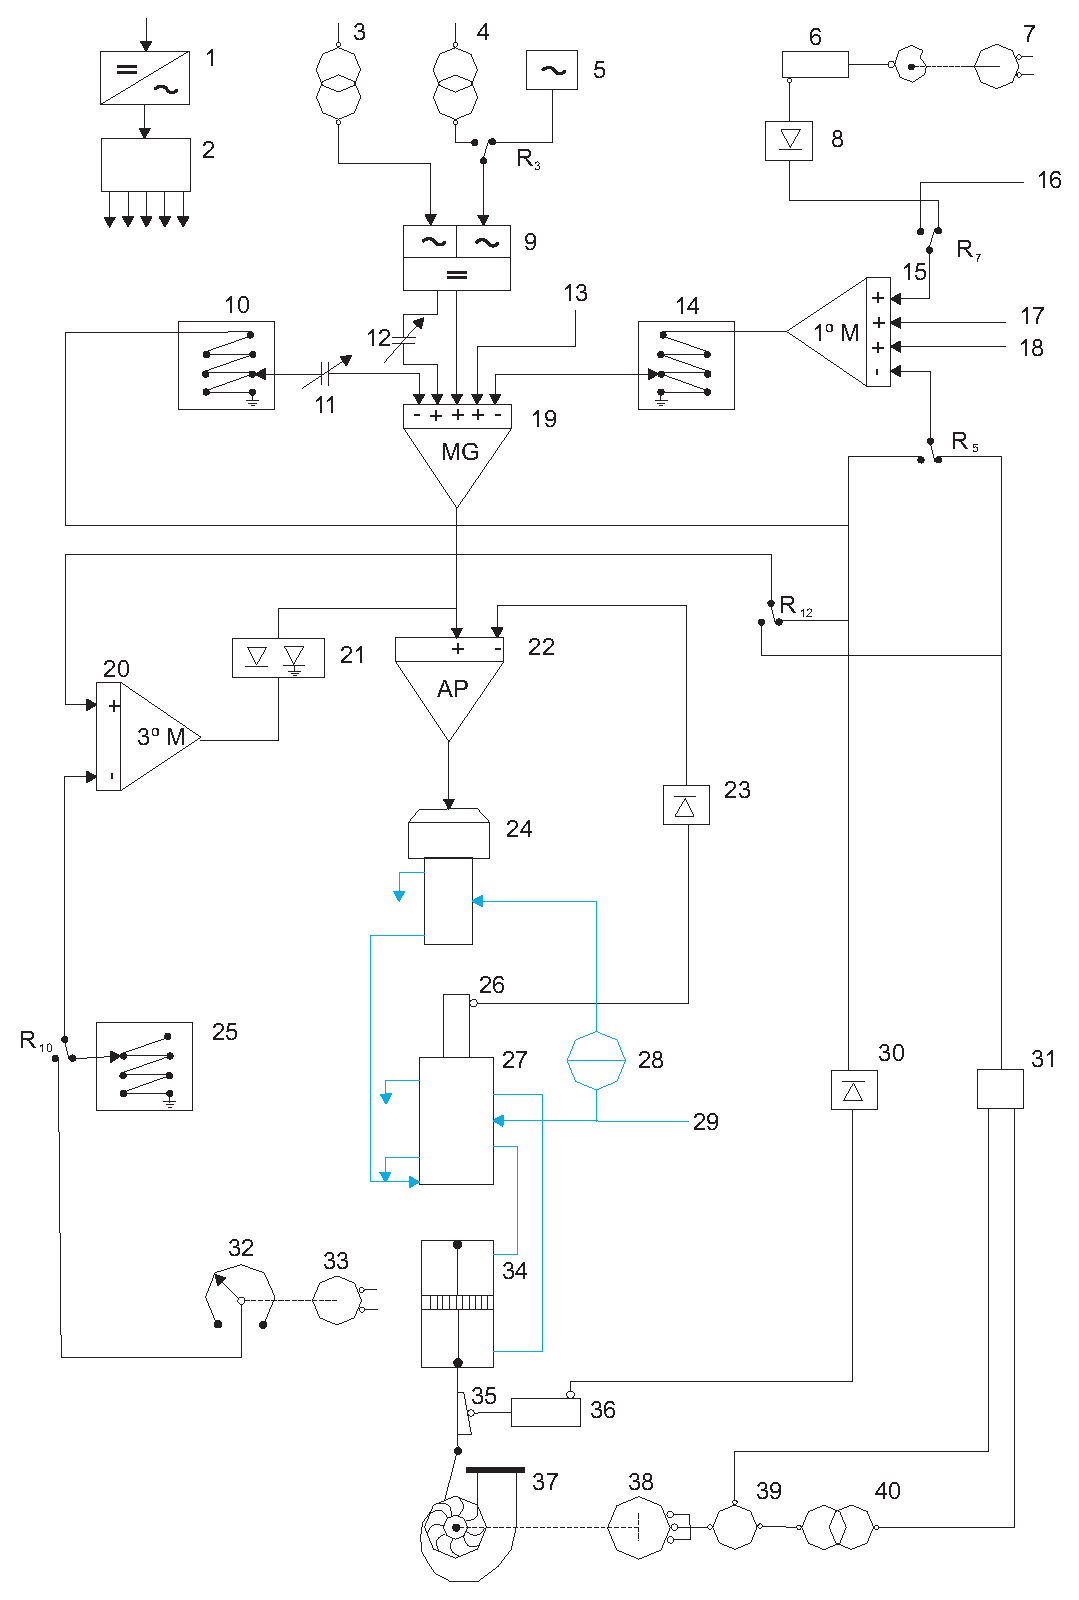
\includegraphics[width=1.0\linewidth]{chapters/introduction/figures/esquema-funcional-rv-rapid77.eps}
  \caption{Esquema funcional del conjunto electro-hidr�ulico del regulador.}
  \label{fig:esquema-funcional-rv-rapid77}
\end{center}
\end{figure}



\begin{table}[H]
\begin{center}
\begin{tabular}{|p{0.7cm}|p{6.5cm}|p{0.8cm}|p{7.5cm}|}
	\cellcolor[gray]{0.8} \textbf{Nro.} & \cellcolor[gray]{0.8} \textbf{Descripci�n} & \cellcolor[gray]{0.8} \textbf{Nro.} & \cellcolor[gray]{0.8} \textbf{Descripci�n}\\
	\hline
	1 & Convertidor est�tico  & 24 & Actuador \\
	\hline
	2 & Repartidor de tensi�n & 25 & Polarizaci�n de marcha en vac�o \\
	\hline
	3 & Transformador de tensi�n del grupo & 26 & Vari�metro de retroceso del distribuidor \\
	\hline
	4 & Transformador de tensi�n de la red & 27 & Distribuidor hidr�ulico \\
	\hline
	5 & Cuarzo patr�n de frecuencia & 28 & Filtro de aceite \\
	\hline
	6 & Vari�metro de carga - frecuencia & 29 & Circuito hidr�ulico de regulaci�n \\
	\hline
	7 & Motoreductor & 30 & Detecci�n \\
	\hline
	8 & Detecci�n & 31 & Transductor vatim�trico \\
	\hline
	9 & Circuito frecuencim�trico & 32 & Potenci�metro de consigna del limitadorde abertura \\
	\hline
	10 & Regulaci�n del estatismo transitorio & 33 & Moto reductor \\
	\hline
	11 & Regulaci�n del Tr del estatismo transitorio & 34 & Servomotor \\
	\hline
	12 & Regulaci�n del Tv del aceler�metro & 35 & Leva \\
	\hline
	13 & Orden exterior & 36 & Vari�metro de retroceso del servomotor \\
	\hline
	14 & Regulaci�n del estatismo permanente & 37 & Turbina \\
	\hline
	15 & Primer mezclador & 38 & Alternador \\
	\hline
	16 & Programa & 39 & TC del alternador \\
	\hline
	17 & Teleregulaci�n & 40 & TP del alternador \\
	\hline
	18 & Orden exterior & R3 & Rel� de sincronizaci�n \\
	\hline
	19 & Mezclador general & R5 & Elecci�n de retroalimentaci�n de potencia o de abertura \\
	\hline
	20 & Comparador limitador & R7 & Programa o carga - frecuencia \\
	\hline
	21 & Circuito limitador & R10 & En reposo antes de acoplar \\
	\hline
	22 & Amplificador de potencia & R12 & Elecci�n entre limitador de abertura o de potencia \\
	\hline
	23 & Detecci�n  &  &  \\
	\hline
\end{tabular}
\caption{Descripci�n de �tems del esquema funcional del conjunto electro-hidr�ulico del regulador}
\label{table:esquema-funcional-rv}
\end{center}
\end{table}








 
\chapter{Planteamiento del problema}

\label{cap:planteamiento-del-problema}

%En este cap�tulo hablo del problema a ser resuelto.
%\include{chapters/sample}
%\section{Introduction}
%For comming\ldots
\section{Introducci�n}

Este cap�tulo plantea el problema abordado en esta investigaci�n: el dise�o de
los modelos de nodos l�gicos y servicios de comunicaci�n a 
ser utilizados en el sistema de regulaci�n de velocidad de una
unidad generadora t�pica de Itaipu. El 
planteamiento del problema se realiza a trav�s de 
una serie de requisitos que debe cumplir el dise�o. 
Estos requisitos fueron formulados 
despu�s de la finalizaci�n del anteproyecto y,
una vez obtenidos los conocimientos m�s 
relevantes de la norma IEC 61850. Es 
el resultado del an�lisis del sistema.

El proceso de ingenier�a IEC 61850 
en centrales hidroel�ctricas 
presenta nuevos retos que no se encuentran 
en el �mbito de subestaciones. Los 
desaf�os encontrados son citados en este cap�tulo.


\section{Requisitos del dise�o}

En esta secci�n se identifican las necesidades 
y condiciones que debe
satisfacer el dise�o del modelo de nodos l�gicos 
y servicios de comunicaci�n de los sistemas 
de automatizaci�n del regulador de velocidad.
Estos requisitos fueron elaborados acorde 
a las directrices de gerenciamiento
de proyecto dadas en la IEC 61850--3 \cite{IEC61850-4:2002} y procedimientos
b�sicos recomendados para la especificaci�n de 
requisitos de software conforme a la norma IEEE 830 \cite{IEEE:830-1998}  
(En la ingenier�a de software se utiliza el 
t�rmino \emph{``Especificaci�n de requisitos de software''} 
para contenidos similares a esta secci�n, 
sin embargo, 
en este trabajo se utiliza simplemente el 
t�rmino \emph{``Requisitos del dise�o''}
o \emph{``Definici�n de los requisitos de dise�o''} 
debido a que en el contexto de la 
automatizaci�n de sistemas de energ�a el�ctrica el t�rmino 
\emph{``Especificaci�n''} es utilizado 
con un significado y un contexto bien definidos, 
distintos a lo expuesto en esta secci�n). 

%\todo[inline]{Leer http://bloqnum.com/pfc/proyecto/node11.html} 


\subsection{Requisitos para la obtenci�n del dise�o de este modelo en
conformidad con la norma IEC 61850}
	\begin{itemize}
	  \item Los nodos l�gicos deben ser obtenidos de las partes 7--4
	  \cite{IEC61850-7-4:2003} y 7--4--10 \cite{IEC61850-7-410:2007} de la norma
		IEC 61850.
	  \item Las nomenclaturas t�cnicas para la designaci�n de los objetos 
	  en los dise�os de ingenier�a y la identificaci�n de se�ales \cite[cl.
	  8.4]{IEC61850-6:2004} deben estar en armon�a con las directrices definidas
	  por la Itaipu Binacional en el marco de actualizaci�n tecnol�gica de la
	  central. En el caso que no sea posible obtener dichas
	  informaciones se utilizar� la norma IEC 61346 \cite{IEC61346-1:1996} para el
	  efecto.
	  \item Los archivos SCL generados durante el proyecto deben ser validados
	  acorde al XML Shema definido en la norma IEC 61850-6 \cite{IEC61850-6:2004}.
 	  Para este trabajo, no es requisito la conformidad con los Tissues
 	  \cite{IEC61850:tissues}.
	\end{itemize}

\subsection{Requisitos tecnol�gicos}
Los dise�os realizados en este trabajo, en la medida de lo  posible,  deben
tener en cuenta el estado del arte de 
las implementaciones de la norma IEC 61850 existentes en el
mercado (para subestaciones, debido a que a�n no existen implementaciones
comerciales de los nodos l�gicos de monitoreo y control para hidroel�ctricas).
La identificaci�n (a grandes rasgos) de los problemas t�cnicos existentes para
la fabricaci�n de dispositivos que implementen 
las definiciones de la norma IEC 61850 ayuda al
proceso de especificaci�n de equipos, pues de esta forma  
el mercado podr� ofertar el producto deseado en los plazos 
establecidos. \footnote{No todos los nodos l�gicos ni servicios de comunicaci�n
definidos por la norma IEC 61850 est�n implementados en el mercado}

Para ello, las siguientes consideraciones son necesarias:
	\begin{itemize}
      \item Identificaci�n de los servicios de comunicaci�n
      definidos por la norma IEC 61850 que ya est�n 
      implementados en dispositivos totalmente funcionales
      y disponibles en el mercado, o bien est�n en proceso 
      de consolidaci�n.
      \item Los nodos l�gicos podr�n ser utilizados en su totalidad, sin
      limitarse a la utilizaci�n de nodos l�gicos disponibles en el mercado,
      debiendo evitarse en lo posible la utilizaci�n de los 
      nodos l�gicos del grupo G de la 
      IEC 61850-7-4 \cite[cl. 5.7]{IEC61850-7-4:2003} si existen los nodos
      l�gicos especializados, adecuados para el efecto \footnote{Dicho
      requisito se debe a que la utilizaci�n de 
      los nodos l�gicos gen�ricos pierden las definiciones
      sem�nticas (congruencia de la informaci�n en t�rminos y significado) 
      que se intenta establecer con la implementaci�n de los nodos
      l�gicos especializados definidos en toda la 
      IEC 61850--7--4--x \cite{IEC61850-7-4:2003}, \cite{IEC61850-7-410:2007},
      \cite{IEC61850-7-420:2009}, \cite{IEC61850-7-430:200-X} }.
      \item En caso que no existan los nodos l�gicos que cubran las
      necesidades del dise�o del modelo del regulador de velocidad de Itaipu se
      se deber� proponer la extensi�n o complementaci�n de los nodos l�gicos de
      la norma IEC 61850.
    \end{itemize}

\subsection{Requisitos para la documentaci�n del dise�o}
Se requiere documentar adecuadamente todo el proceso de ingenier�a aplicado
durante el proyecto a trav�s de:
	\begin{itemize}
      \item Planos de la arquitectura referencial del sistema y del modelo IEC
      61850.
	  \item Tablas de la plantilla de los nodos l�gicos utilizados, identificando
	  inclusive los Data Objects seleccionados.
	  \item Descripci�n formal en SCL de la plantilla de los nodos l�gicos
	  utilizados, identificando los Data Objects seleccionados.
	  \item Tablas de las instancias de los nodos l�gicos, en sus correspondientes
	  Logical Devices e IEDs.
	  \item Descripci�n formal en SCL de las instancias de los nodos l�gicos, en
	  sus correspondientes Logical Devices e IEDs.
	\end{itemize}
\section{Desaf�os encontrados al realizar el dise�o}

Debido a que durante el transcurrir de este trabajo no se ha encontrado en el
mercado ning�n IED regulador de velocidad de turbinas hidroel�ctricas que
implemente la norma IEC 61850-7-4-10 \cite{IEC61850-7-410:2007} se ha vuelto 
dif�cil hallar un punto de partida para 
definir los procesos de ingenier�a adecuados para el efecto. De
hecho, las herramientas de ingenier�a tampoco proporcionan un soporte completo
para los proyectos IEC 61850 en hidroel�ctricas.      

Otro problema importante fue la falta literatura sobre la norma IEC
61850--7--4--10 \cite{IEC61850-7-410:2007}. A la fecha de culminaci�n de este
trabajo no se encontraban disponibles documentos p�blicos oficiales publicados por la IEC que describan
la combinaci�n adecuada de los nodos l�gicos definidos por la norma IEC
61850--7--4--10 \cite{IEC61850-7-410:2007} para conformar las funciones de
monitoreo y control correspondientes. En el 
�mbito de subestaciones las cl�usulas 8, 9 y 11 de la
IEC 61850--5 \cite{IEC61850-5:2003} proveen un punto de partida muy importante
para el modelado de las funciones del 
sistema gracias a la combinaci�n correcta de los nodos l�gicos
definidos en la IEC 61850--7--4 \cite{IEC61850-7-4:2003}. El autor de este
trabajo tiene entendido que los documentos oficiales que describen aspectos relevantes 
del  dise�o de modelos de sistemas IEC 61850 para hidro�ctricas est�n en proceso
de elaboraci�n, y ser�n publicados bajo la serie IEC 61850--7--510 \cite{IEC61850-7-510:2009}.

%\section{Justificativa de la realizaci�n del trabajo}
\section{Importancia de la resoluci�n del problema propuesto}


La norma IEC 61850 define un modelo de informaci�n capaz de ajustarse a
filosof�a de la empresa generadora de energ�a. Debido a ello, la definici�n de
las plantillas de tipos de datos basados en las definiciones de modelos de
informaci�n de la norma IEC 61850 y sus respectivas instancias implementadas en
el sistema de monitoreo y control que se adapten al desempe�o particularmente
estricto de la regulaci�n de velocidad de las unidades generadoras de Itaipu,
que son muy importantes para el sistema interconectado Paraguay--Brasil,
contribuyen al proceso de ingenier�a IEC 61850 que formar�a parte de la
especificaci�n de los nuevos IEDs reguladores de velocidad que ser�n adquiridos
en el marco de actualizaci�n tecnol�gica de la Itaipu Binacional.            

\chapter{Enfoque del proceso de ingenier�a IEC 61850 
propuesto por el autor para la resoluci�n del problema} 
\label{ch:enfoque-del-autor}
 

\section{Introducci�n}

La norma IEC 61850 propone, de manera flexible, 
una serie de pasos alternativos para abordar el proceso 
de construcci�n de los sistemas y redes de comunicaci�n 
en las subestaciones. Un mismo problema puede ser resuelto 
de diversas maneras, y esto puede ser evidenciado 
analizando el flujo de trabajo propuesto por las 
herramientas de ingenier�a disponibles actualmente 
en el mercado.



%Este cap�tulo describe como el autor 
%de este trabajo ha resuelto 
%el problema descripto en el 
%cap�tulo \ref{cap:planteamiento-del-problema}.

Tras la experiencia obtenida 
en el PTI durante la realizaci�n 
de este trabajo \cite{PTI:SESEP2010}, 
el autor ha seleccionado  
el proceso de ingenier�a que m�s se adapte 
a las necesidades encontradas para 
la elaboraci�n del modelo adecuado 
para los sistemas de comunicaci�n y redes 
del regualdor de velocidad de una unidad generadora 
t�pica de Itaipu.


El enfoque que se presenta en este cap�tulo 
trata de adecuarse a la realidad del entorno 
de mercado y de los recursos disponibles, 
con el objetivo de obtener un dise�o 
que en un futuro ayude a la construcci�n
del nuevo sistema IEC 61850 en las
unidades generadoras de Itaipu Binacional. 
Un enfoque adecuado permite obtener un dise�o 
que cubra las necesidades reales del sistema,
y haciendo realidad la promesa de la norma IEC 61850:
sistemas a prueba de futuro. 

El dise�o de las plantillas de tipos de datos 
y la definici�n de sus correspondientes instancias en los 
IEDs se puede realizar de diversas formas. El
enfoque presentado en este trabajo tiene como 
objetivo estar en armon�a con el enfoque 
utilizado en la Itaipu Binacional en  
la primera especificaci�n de equipos IEC 61850 
para la linea de 500KV \cite{Itaipu:linea500KV}, 
cuya licitaci�n internacional se ha hecho 
p�blica en octubre del 2010. Adem�s se 
propone enriquecer dicho enfoque con la 
especificaci�n de los Data Objects 
y sus respectivas instancias en IEDs, 
los cuales, seg�n la visi�n del autor de este trabajo, 
ayudar�a a mejorar el dise�o 
de sistemas a prueba de futuro. 

El modelo de informaci�n de la norma IEC 61850 
se clasifica como un sistema 
\gls{O-O-es}. Es necesario tener 
una clara comprensi�n de la tecnolog�a \gls{O-O-es} 
para aplicar correctamente el proceso de ingenier�a
propuesto en este cap�tulo. Por esta raz�n, 
esta secci�n describe en forma bien selectiva la
tecnolog�a \gls{O-O-es} en la cual 
la norma IEC 61850 
se ha apoyado. No se describen todos los principios 
orientados a objetos, s�lo se presentan 
los fundamentos necesarios para entender el modelo 
de informaci�n con el cual se contruy� la 
norma IEC 61850. Se provee una descripci�n detallada de 
los fundamentos del paradigma \gls{O-O-es}  seleccionados
a trav�s de implementaciones pr�cticas en lenguajes de 
programaci�n \gls{O-O-es} populares \cite{Java:specification},  
\glsentrytext{UML-es}  \cite{UML2:2009}
y se proveen materiales de referencia 
para su profundizaci�n.  
















\section{Estado del arte del proceso de ingenier�a IEC 61850}
	\label{sec:ENFOQUE-estado-del-arte-herramientas}

Durante la experiencia adquirida 
con el uso de herramientas de ingenier�a IEC 61850 \cite{PTI:SESEP2010}, 
el autor ha observado que 
el uso de estas herramientas como apoyo a la elaboraci�n
de especificaciones y proyectos ejecutivos es un campo muy nuevo en el �rea de
la ingenier�a el�ctrica. Todas las herramientas disponibles en el mercado se
encuentran en sus primeras versiones estables, y existen muchas teor�as,
discusiones y debates vigentes respecto de las caracter�sticas necesarias en
una herramienta de este tipo para soportar el proceso de ingenier�a IEC 61850.       

Las diversas herramientas tercerizadas existentes en el mercado implementan lo
establecido abstractamente por la IEC61850 usando metodolog�as y flujos de
trabajo diferentes en mayor o menor grado, en ocasiones con interpretaciones
diferentes de lo establecido por la norma. Esto es natural, considerando la
complejidad de la misma y que estas son las primeras implementaciones pr�cticas
disponibles hoy en d�a como productos comerciales. 

Las herramientas Helinks y Visual SCL
proponen utilizar flujos de trabajo similares. Dichas 
herramientas han sido dise�adas para asistir el proceso de
ingenier�a denominado \emph{``Top down engineering''}, 
que consiste b�sicamente en la especificaci�n del sistema 
a trav�s de la variante SSD, la selecci�n e inclusi�n 
de los ICDs que realizen las funciones definidas en el SSD,
y la configuraci�n completa del sistema a trav�s de 
la variante SCD donde se realizan referencias cruzadas 
entre los archivos ICD y el SSD.

La herramienta H\&S STS fue dise�ada para trabajar con 
el mismo flujo de trabajo que las dos herramientas arriba 
mencionadas, pero como paso alternativo, propone
que el proyectista dise�e los 
de ICDs en modo gr�fico a partir del SSD, 
para especificar los IEDs (con sus ICDs)
a ser comprados para el proyecto. De hecho, esto tambi�n puede
ser realizado en las herramientas anteriores, pero no fueron 
optimizadas para ello, por lo tanto, no dan mucha asistencia 
al proyectista.   

La herramienta Kalkitech SCL Manager tambi�n propone el mismo 
flujo de trabajo que las dos primeras herramientas mencionadas,
y adem�s tiene un m�dulo para crear variantes ICD. 

La herramienta de ingenier�a Atlan61850 propone iniciar 
el proceso de ingenier�a con la inclusi�n de los ICDs 
en el proyecto, omitiendo el uso de la variante SSD, 
y creando directamente los CIDs
correspondientes. A este enfoque se lo denomina
\emph{``Bottom up engineering''}.

El autor de este trabajo ha analizado las posiblidades de 
utilizar estas herramientas durante el proceso de ingenier�a,
pero debido a las dificultades encontradas (Helinks no posee 
el nodo l�gico \textbf{KTNK}, en la versi�n demo de Kalkitech SCL Manager
no es posible guardar el proyecto, en la versi�n demo de H\&S STS
se habilitan menos de una decena de nodos l�gicos de subestaciones,
y la herramienta Atlan61850 acepta los ICDs y XSDs desarrollados por el 
autor pero requiere la profundidad del ICD hasta los \textbf{DAI}
para manejar todos los puntos del sistema)
el autor no ha utilizado una sola herramienta, 
sino que utiliza un enfoque mixto 
usando varias herramientas para definir un nuevo enfoque, 
adecuado al problema planteado, que ser� explicado en este cap�tulo.


\section{Documentaci�n autom�tica de este trabajo}
\label{sec:doc-automatica}

La norma IEC 61082 \cite{IEC61082-1:2004} recomienda una serie de
principios para la generaci�n 
autom�tica de documentos sobre electrotecnolog�a.

Las ventajas de este enfoque son muy claras:
\emph{``Cuando la informaci�n es guardada en un formato 
independiente de cualquier presentaci�n, 
esta informaci�n puede ser accesible 
con diferentes vistas y formatos en el momento 
en que sea necesitado y en la forma m�s adecuada 
para los fines previstos.''} \cite{IEC61082-1:2004}

El proceso puede ser observado en la 
figura \ref{fig:Enfoque-documentos-generados-iec61082.eps}. 

\begin{figure}
\begin{center}
  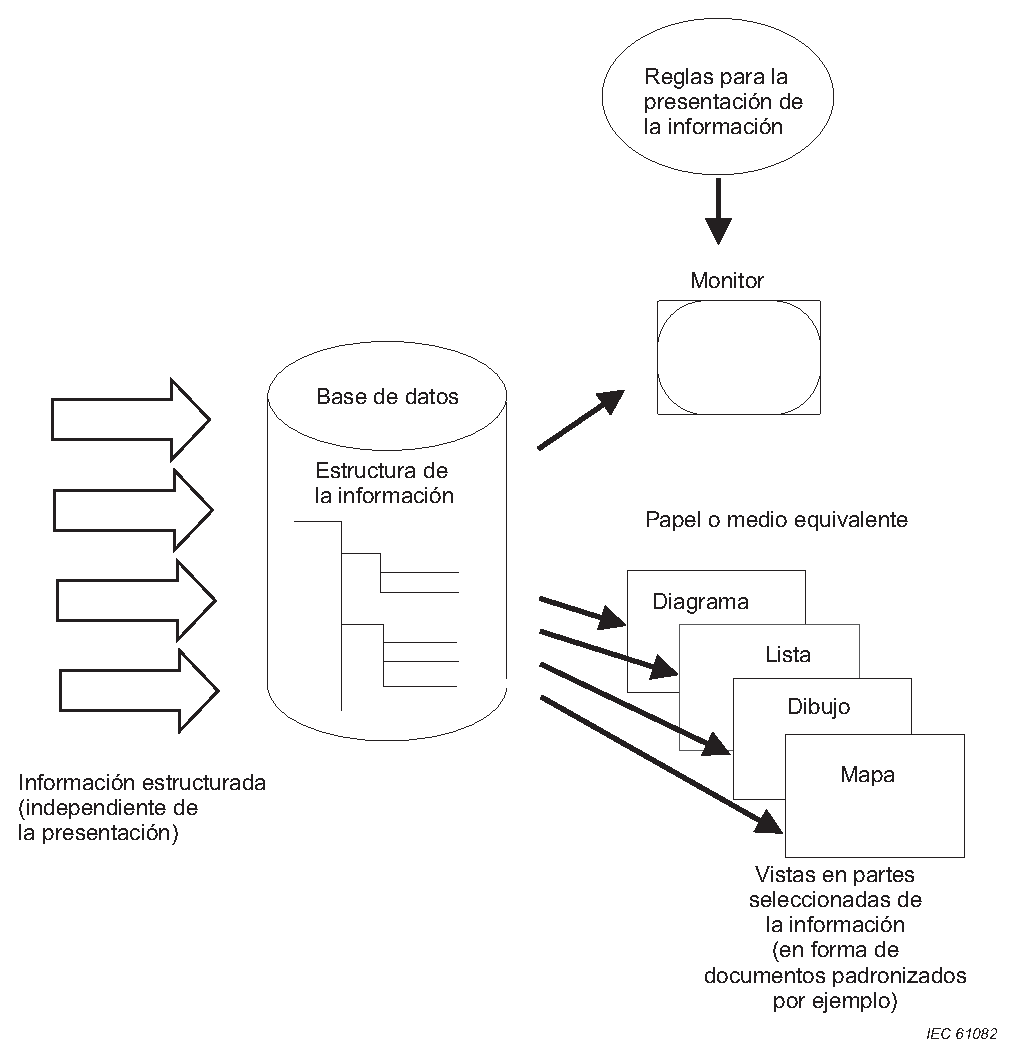
\includegraphics[width=1.0\linewidth]{chapters/enfoque/figures/documentos-generados-iec61082.eps} 
  \caption{Enfoque propuesto por la norma IEC 61802 para la generaci�n de
  documentos sobre electrotecnolog�a} 
  \label{fig:Enfoque-documentos-generados-iec61082.eps}
\end{center}
\end{figure}

Considerando que el \gls{SCL} permite expresar de 
manera formal todo 
el proyecto IEC 61850,
resulta muy sencillo realizar la documentaci�n autom�tica
de este proyecto. Es posible leer los archivos \gls{SCL}
donde se encuentran los modelos de informaci�n
mediante lenguajes de programaci�n que provean librer�as
para la lectura de archivos XML. En este trabajo se ha
utilizado el lenguaje de programaci�n orientado a 
objetos \emph{Python 2.6},
que a partir de los ICDs dise�ados durante
el proceso de ingenier�a,
ha generado en forma autom�tica 
las tablas del cap�tulo \ref{cap:model},
siguiendo las recomendaciones de la norma IEC 61082 \cite{IEC61082-1:2004}

Por lo tanto, de aqu� en m�s, todo el proceso de ingenier�a 
utilizado en este trabajo 
expresa el flujo de trabajo y
los dise�os en t�rminos de \gls{SCL}, 
y los gr�ficos se presentan  
como complemento.




\section{Virtualizaci�n IEC 61850 de unidades generadoras de centrales hidroel�ctricas}
%\ref{sec:Modelo-informacion-61850}

Existen dos posibles enfoques para la definici�n de los 
nodos l�gicos de un sistema IEC 61850:
\begin{enumerate}
  \item Definici�n de los modelos de nodos l�gicos 
  de los puntos de comunicaci�n entre dispositivos IEC 61850.
  \item Definici�n de los modelos de nodos l�gicos 
  de los puntos de comunicaci�n entre dispositivos IEC 61850, 
  y virtualizaci�n IEC 61850 de toda la planta (incluso si el 
  dato no ser� transmitido por la red).
\end{enumerate}


\begin{figure}
\begin{center}
  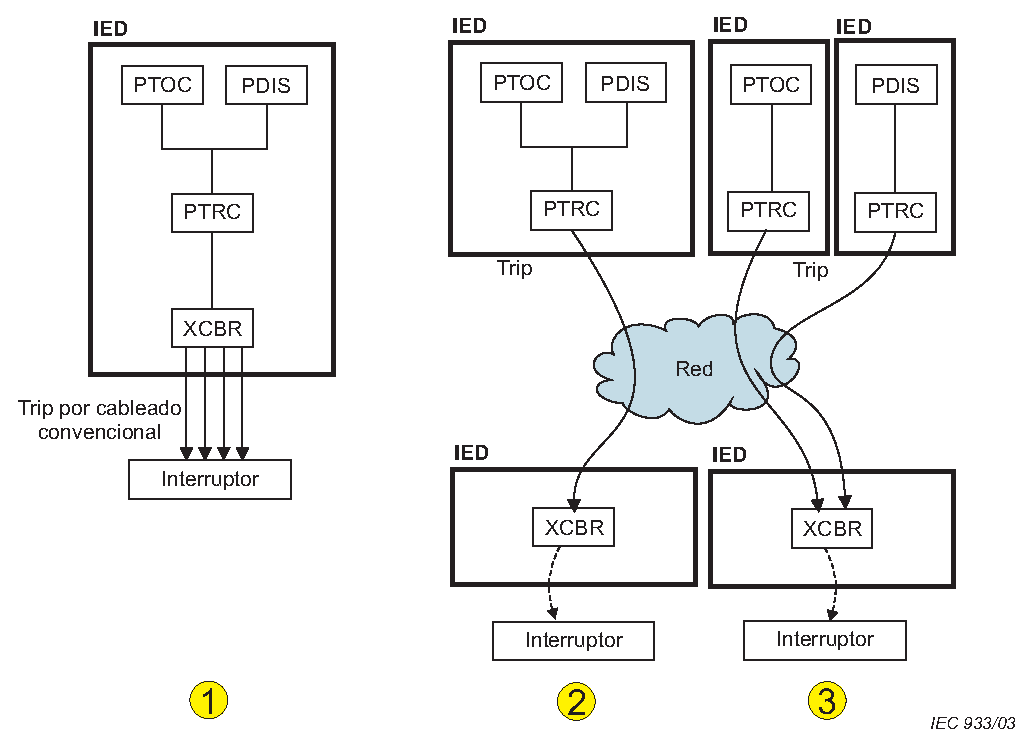
\includegraphics[width=1.0\linewidth]{chapters/enfoque/figures/virtualizacion-CBR.eps}
  \caption{Virtualizaci�n de un interruptor}
  \label{fig:virtulization-CBR}
\end{center}
\end{figure}



En el presente trabajo se opta por dise�ar el 
modelo conforme al segundo enfoque mencionado arriba. Este enfoque
presenta muchas ventajas, dado que se dota al sistema 
de una sem�ntica muy detallada de toda la planta. Una primera 
aproximaci�n puede ser observada en la figura
\ref{fig:virtualizacion-hydro-presa}.

\begin{figure}
\begin{center}
  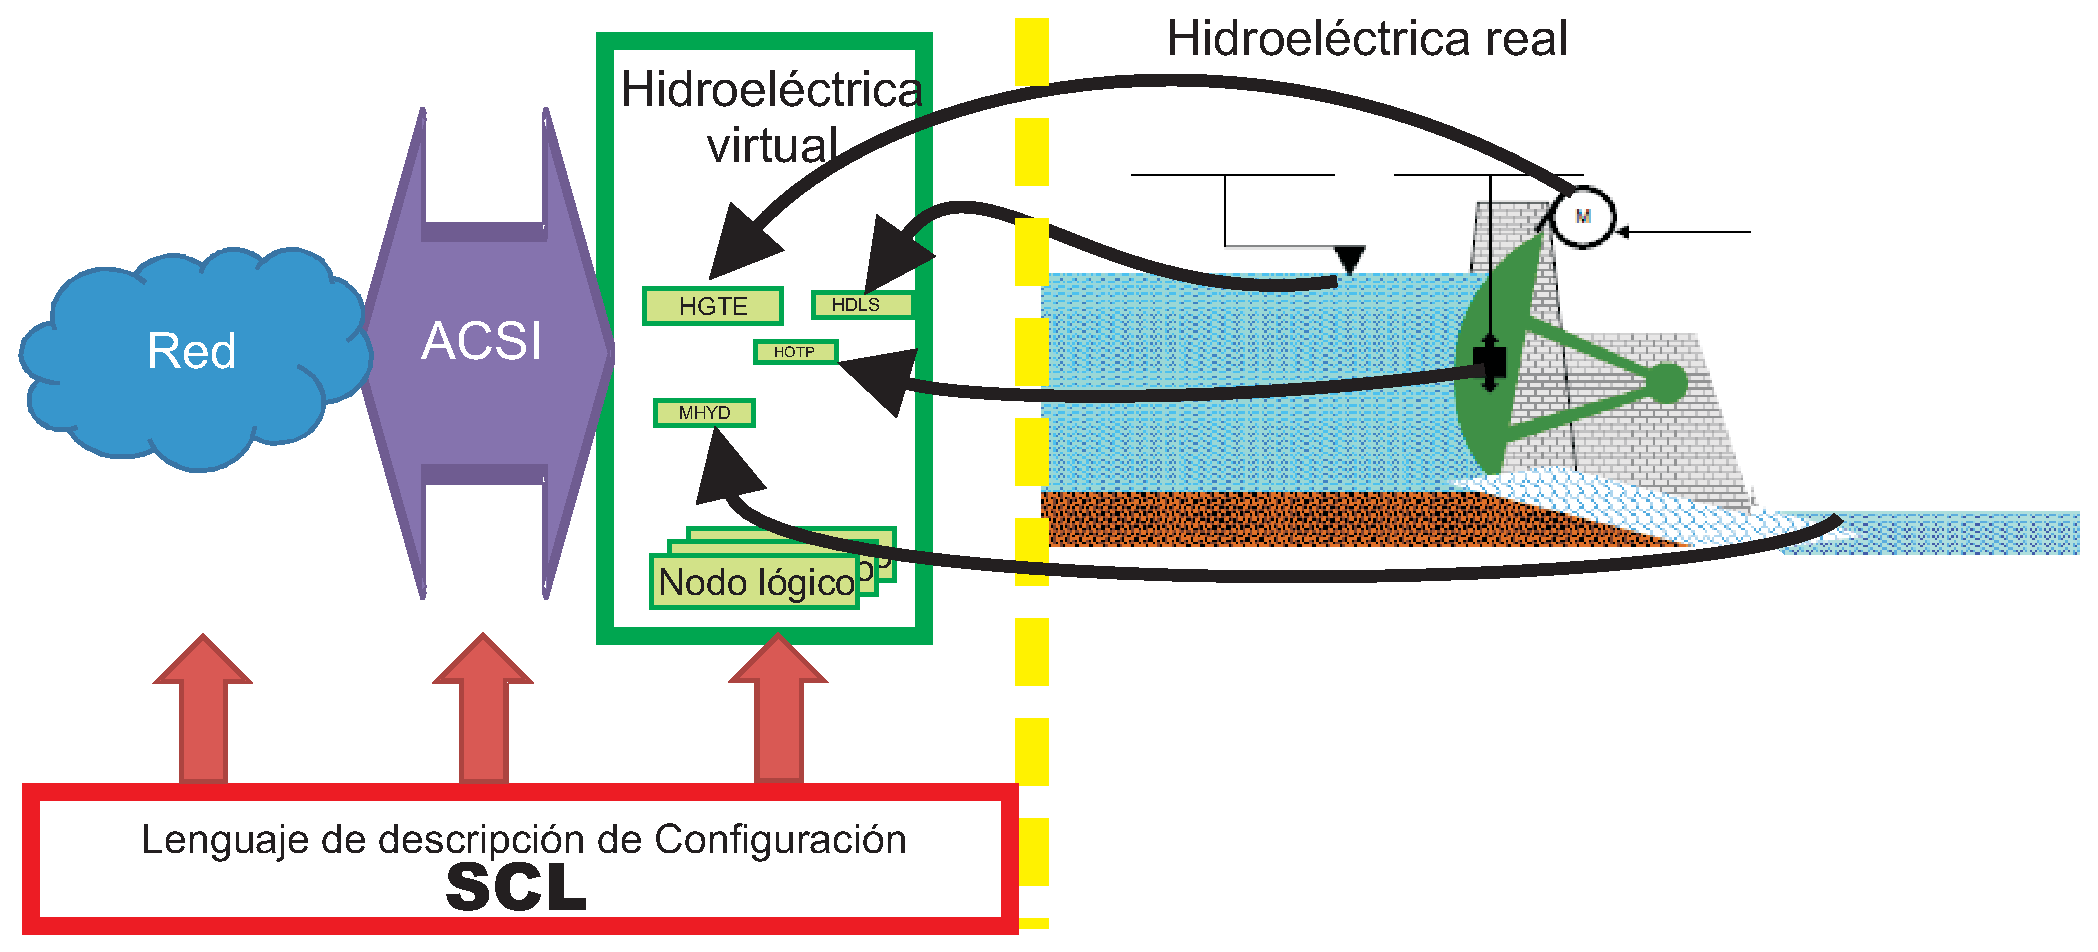
\includegraphics[width=1.0\linewidth]{chapters/enfoque/figures/virtualizacion-hydro-presa.eps}
  \caption{Virtualizaci�n IEC 61850 de una central hidroel�ctrica}
  \label{fig:virtualizacion-hydro-presa}
\end{center}
\end{figure}



En la figura \ref{fig:virtulization-CBR} obtenida
del apartado IEC 61850--7--1 \cite{IEC61850-7-1:2003} se observa,
un interruptor virtualizado con el nodo l�gico \textbf{XCBR}. En el 
caso (1) el interruptor f�sico recibe comunicaci�n del IED (que se puede 
encontrar a nivel de bay, por ejemplo)
a trav�s de cableado convencional, y el IED puede utilizar 
el nodo l�gico \textbf{XCBR} para activar los 
comandos de apertura o cierre, de acuerdo a 
las condiciones de trip definidos en el nodo l�gico
\textbf{PTRC}. En el mercado existen IEDs que permiten 
asignar a los contactos f�sicos binarios los 
comandos de apertura o cierre v�a cableado convencional, 
como as� tambi�n existen IEDs que tienen los nodos l�gicos
desde el \textbf{PTOC} por ejemplo, hasta el \textbf{PTRC},
pero sin incluir el \textbf{XCBR}, pero permitiendo 
el accionamiento del interruptor por cableado convencional. Para 
este tipo de IEDs se pierde parte de la sem�ntica que podr�a 
obtenerse con la virtualizaci�n del interruptor. En caso de 
que se tenga el nodo l�gico \textbf{XCBR}, siempre considerando 
el caso 1 de la figura \ref{fig:virtulization-CBR},
se pueden utilizar datos sem�nticos por norma (del \textbf{XCBR}) 
en las l�gicas del IED (que se encuentran fuera del alcance de la norma IEC
61850), con lo que la complejidad del \gls{SAS} se simplifica.

En los casos (2) y (3) de la figura \ref{fig:virtulization-CBR} 
se pueden observar como se distribuye una funci�n del \gls{SAS}
entre varios IEDs. El hecho de poseer un modelo de nodos l�gicos 
que incluya el \textbf{XCBR} para este ejemplo, 
disminuir�a considerablemente los cambios en el proyecto
para en un futuro migrar la funci�n centralizada (caso 1)
a una funci�n distribuida entre varios IEDs (casos 2 y 3).

Este mismo principio
es totalmente aplicable en el dise�o de modelos IEC 61850 de 
hidroel�ctricas, y 
vuelve a ser esbozado en el apartado 
IEC 61850--7--4--10 \cite{IEC61850-7-410:2007} a trav�s 
de la figura \ref{fig:virtulization-potenciometro}, donde 
se puede visualizar la virtualizaci�n de la interfaz
f�sica con un potenci�metro motorizado a trav�s 
del nodo l�gico \textbf{FSPT}, que es utilizado, entre otras cosas, para indicar valores de funciones de control.

\begin{figure}
\begin{center}
  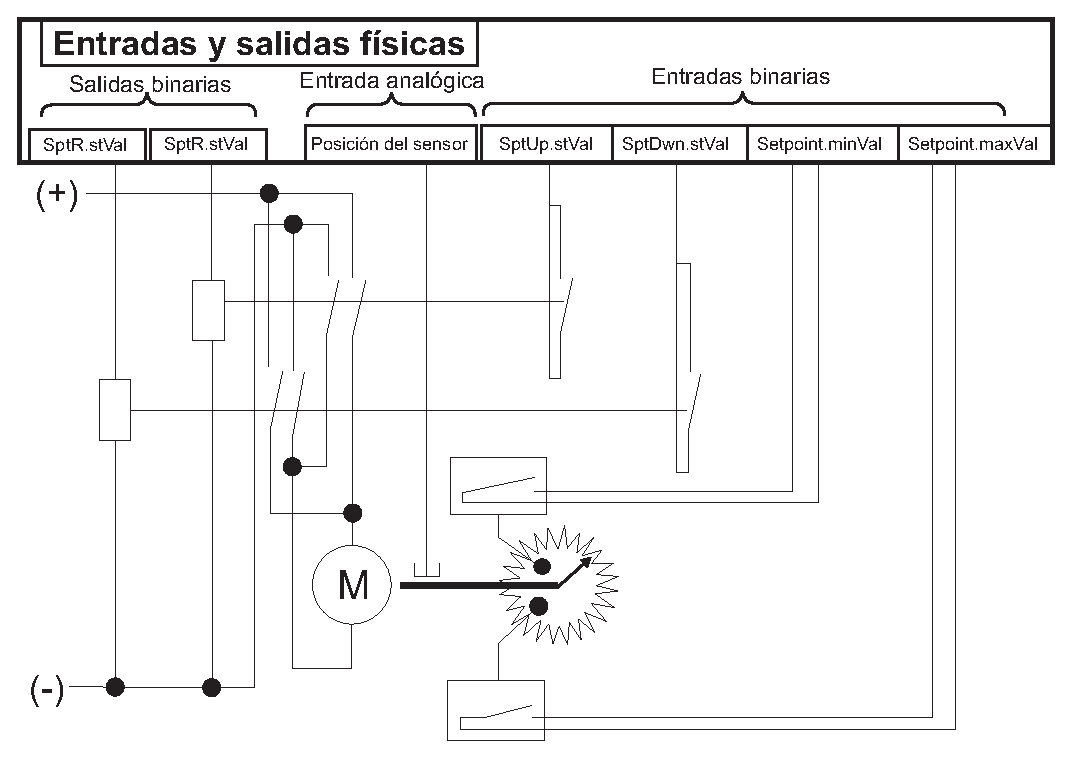
\includegraphics[width=1.0\linewidth]{chapters/enfoque/figures/virtualizacion-potenciometro.eps}
  \caption{Virtualizaci�n de una interfaz f�sica con un potenci�metro
  motorizado}
  \label{fig:virtulization-potenciometro}
\end{center}
\end{figure}

Entonces, siguiendo este enfoque, se han virtualizado 
numerosos datos del sistema a trav�s de nodos l�gicos 
que contienen el \gls{CDC} \textbf{SAV}, que es 
utilizado para bus de proceso. Si bien no se 
utilizar� el bus de proceso para todos los nodos l�gicos que contengan \textbf{CDCs} \textbf{SAV}, 
se aplica el mismo principio de virtualizaci�n del 
interruptor (\textbf{XCBR}) explicado en los p�rrafos anteriores.

Los principales nodos l�gicos de la 
norma IEC 61850--7--4--10 \cite{IEC61850-7-410:2007} 
que est�n compuestos por \textbf{CDCs} \textbf{SAV}
son los del grupo T. Es posible observar 
la interacci�n de este nodo l�gico con 
los nodos l�gicos del bus de estaci�n en la figura
\ref{fig:LN-bus-proceso-7-4-10}, obtenida de \cite{IEC61850-7-410:2007}.

\begin{figure}
\begin{center}
  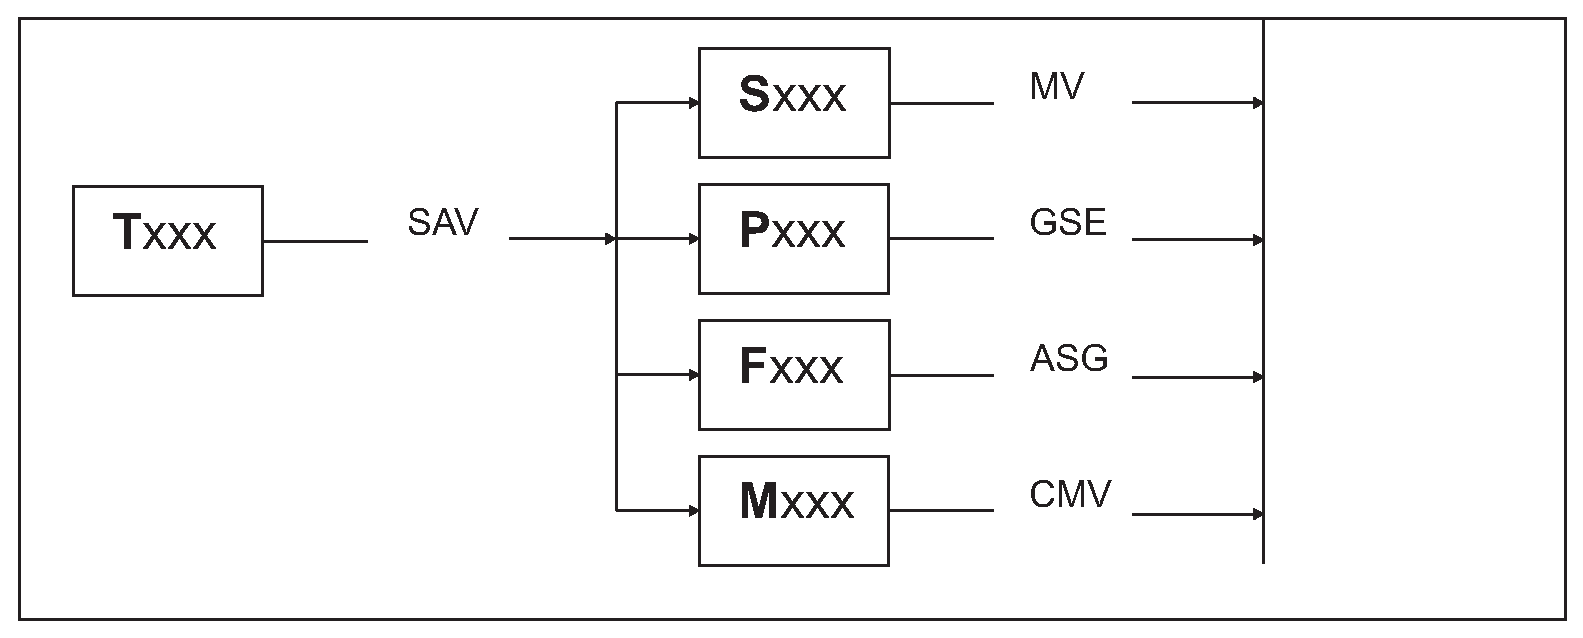
\includegraphics[width=1.0\linewidth]{chapters/enfoque/figures/virtualizacion-LNs-con-SAV.eps}
  \caption{Los nodos l�gicos del grupo T utilizan el bus de proceso (IEC
  61850--9--x)}
  \label{fig:LN-bus-proceso-7-4-10}
\end{center}
\end{figure}


\section{Proceso de ingenier�a totalmente basado en SCL}

%El uso adecuado del \gls{SCL} durante el 
%proceso en ingenier�a trae grandes ventajas 

El flujo de trabajo a ser adoptado durante el proceso
de ingenier�a IEC 61850 de una subestaci�n 
permite dise�ar el sistema 
acorde a lo indicado en el 
apartado IEC 61850--7--1 \cite[cl. 6]{IEC61850-7-1:2003},
\cite[cl. 7.2]{IEC61850-7-1:2003},  
\cite[cl. 8.2]{IEC61850-7-1:2003}.
Todo el dise�o del sistema se puede describir mediante el \gls{SCL}, 
siguiendo los pasos indicados en el apartado 
IEC 61850--6 \cite[cl. 5]{IEC61850-6:2004},
siempre considerando los requisitos 
que exige el dise�o, seg�n las definiciones 
del apartado IEC 61850--4 \cite[cl. 5]{IEC61850-4:2002}.


El \gls{SCL} es  
la parte m�s importante de la 
serie IEC 61850 \cite{Schwarz:2007}, 
pues todo el proceso de ingenier�a 
puede apoyarse en este lenguaje. Todas 
las dem�s partes de la norma (correspondientes 
al dise�o de sistemas), pueden ser expresadas a trav�s 
del \gls{SCL}. 


Durante el transcurrir de este cap�tulo 
se demuestra la viabilidad t�cnica de la 
utilizaci�n del \gls{SCL} durante todo el proceso de 
ingenier�a IEC 61850.


Como primer paso para dicha demostraci�n,
es imprescindible identificar 
el modelo de informaci�n
del sistema que puede ser 
dise�ado mediante \gls{SCL} y  
sus respectivas reglas de
utilizaci�n.
Aplicando 
ingenier�a inversa a 
los XSDs \cite{Hypermodel:2010} de 
IEC 61850-6 \cite{IEC61850-6:2004} es posible 
visualizar con mayor facilidad 
los \textbf{SCL XML Shemas} a trav�s del \gls{UML-es}. 

A medida que en este cap�tulo se van identificando 
las posibilidades 
que ofrece el \gls{SCL}, el autor concibe
el enfoque m�s adecuado 
para resolver el problema planteado.


\section{Descripci�n del modelo IEC 61850 orientado a objetos mediante SCL}
El \gls{SCL}, como se ha mencionado 
en los cap�tulos introductorios,
define b�sicamente 5 grandes partes:
\begin{enumerate}
  \item Header
  \item Substation
  \item Communication
  \item IED
  \item DataTypeTemplates 
\end{enumerate}  
La representaci�n en \gls{UML-es} de estas 5
partes mencionadas es presentada en la 
figura \ref{fig:SCL-main-parts}.
 
\begin{figure}
\begin{center}
  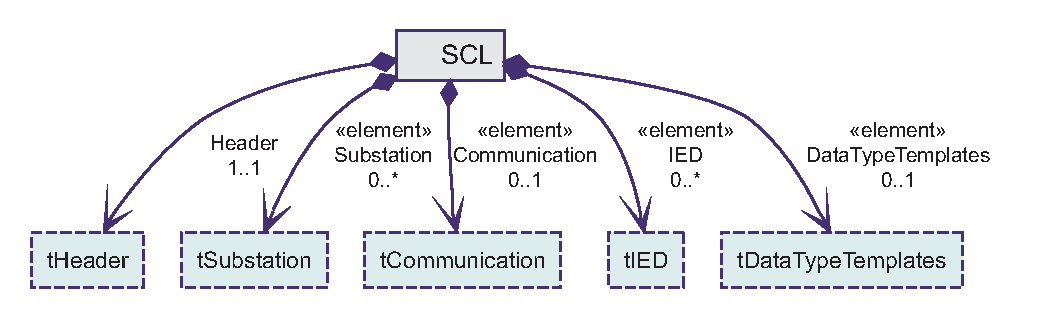
\includegraphics[width=1.0\textwidth]{chapters/enfoque/figures/scl-depth2-heredado.eps}
  \caption{Partes principales del SCL}
  \label{fig:SCL-main-parts}
\end{center}
\end{figure}

Antes de explicar estas partes 
con la profundidad adecuada, 
es necesario 
formular una definici�n precisa 
del paradigma \gls{O-O-es}. Muchos 
autores ya han formulado definiciones 
precisas  
\cite{Rentsch:1982} 
\cite{Pascoe:1986}
\cite{Nygaard:1986}
\cite{Madsen:1988}, 
y la definici�n de Lastly, Wegner
\cite{Wegner:1987} ha sido 
la m�s aceptada \cite{Capretz:2003}.
Wegner define el paradigma \gls{O-O-es} 
en t�rminos de objetos, clases y herencia.

\emph{
	`` Los objetos son entidades aut�nomas
	que responden a mensajes u operaciones y
	comparten un estado. Las clases clasifican
	objetos por sus operaciones comunes.
	La herencia sirve para clasificar clases 
	con respecto a su comportamiento com�n. La 
	abstracci�n de datos esconde (simplifica) la 
	representaci�n de datos y su implementaci�n 
	de operaciones '' 
}\cite{Wegner:1987}. Esto es: 

\begin{center}
	orientado a objetos = objetos + clases + herencia
\end{center}

%Estos conceptos En las siguientes secciones

La metodolog�a que utiliz� la norma IEC 61850 
para la creaci�n del \gls{SCL} y los modelos de 
informaci�n definidos formalmente en IEC 61850--7--x 
\cite{IEC61850-7-1:2003}
\cite{IEC61850-7-2:2003}
\cite{IEC61850-7-3:2003}
\cite{IEC61850-7-4:2003}
\cite{IEC61850-7-410:2007} 
enfoca la organizaci�n del modelo
a trav�s de la creaci�n de objetos de la siguiente forma:
Los objetos guardan el dato y tienen un 
comportamiento propio con una forma particular 
para agrupar la informaci�n por funcionalidades comunes 
y estructuras comunes de la informaci�n. 
Este enfoque permite 
empaquetar un conjunto de acciones comunes,
manejar una peque�a cantidad de variables 
en lugar de m�ltiples variables, 
organizar comportamientos comunes agrup�ndolos 
y estructurando los 
sistemas l�gicos de forma a que 
representen al mundo real.



%\subsubsection{Clases}
%\subsubsection{Objetos}





\section{DataTypeTemplates}

El elemento \emph{DataTypeTemplate} 
y todos 
sus elementos hijos ser�an 
lo m�s pr�ximo 
a definiciones de clase. 
Si bien sabemos que 
los archivos XML se utilizan 
generalemente como
mecanismo para la \gls{SO},
en realidad el \emph{DataTypeTemplate} 
es lo m�s cercano a la definici�n de 
clases del paradigma \gls{O-O-es}, 
pues los elementos hijos de
\emph{DataTypeTemplates} 
sirven como plantillas a trav�s 
del cual las instancias son creadas
en un IED. De hecho, tambi�n puede
relacionarse un \emph{DataTypeTemplate}
directamente con el modelo de 
informaci�n inicialmente ubicado 
en el elemento \emph{Substation}, 
pero considerando que el 
SCL XML Schema no define v�nculos 
obligatorios entre el elemento \emph{Substation}
y el elemento \emph{DataTypeTemplate}
(en el elemento \emph{IED} s� lo hace), 
entonces en este trabajo se opt� por 
vincular directamente el \emph{DataTypeTemplate}
con el elemento \emph{IED} de 
cada \gls{ICD}. 
En la figuras 
\ref{fig:SCL-DataTypeTemplates-depthMax-conHerencia}
y
\ref{fig:SCL-DataTypeTemplates-depthMax-heredado}
se pueden observar los diagramas 
de clases del DataTypeTemplate.
Los mismos diagramas, en forma simplificada,
son proveidos en las figuras
\ref{fig:SCL-DataTypeTemplates-depthMax-conHerencia-simplificado}
y 
\ref{fig:SCL-DataTypeTemplates-depthMax-heredado-simplificado}.

\begin{figure}
\begin{center}
  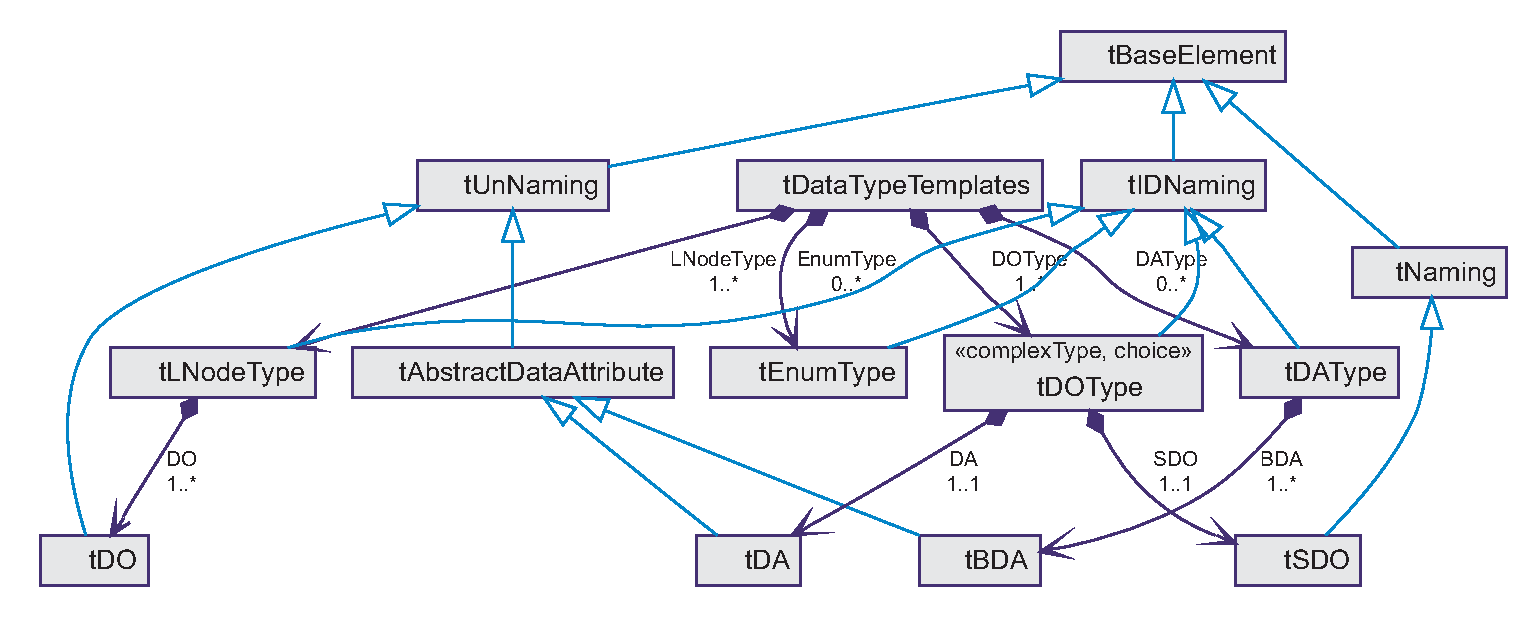
\includegraphics[width=1.0\linewidth]{chapters/enfoque/figures/scl-DataTypeTemplates-depthMax-conHerencia-simplificado.eps} 
  \caption{Diagrama de clases simplificado del elemento \emph{DataTypeTemplate}
  del SCL, incluyendo sus clases abstractas}
  \label{fig:SCL-DataTypeTemplates-depthMax-conHerencia-simplificado}
\end{center}
\end{figure}

\begin{figure}
\begin{center}
  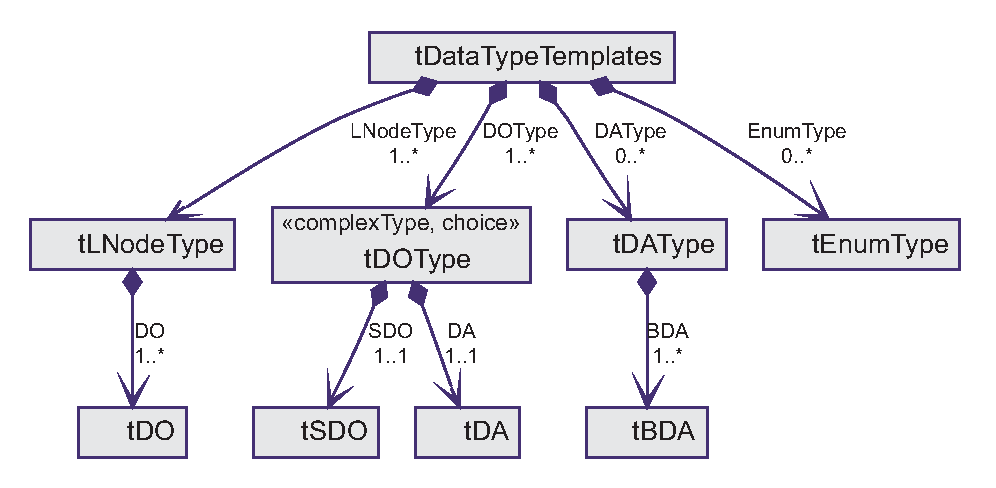
\includegraphics[width=0.7\linewidth]{chapters/enfoque/figures/scl-DataTypeTemplates-depthMax-heredado-simplificado.eps} 
  \caption{Diagrama de clases simplificado del elemento \emph{DataTypeTemplate}
  del SCL, omitiendo sus clases abstractas}
  \label{fig:SCL-DataTypeTemplates-depthMax-heredado-simplificado}
\end{center}
\end{figure}


\begin{landscape}
\thispagestyle{empty}
\begin{figure}
\begin{center}
  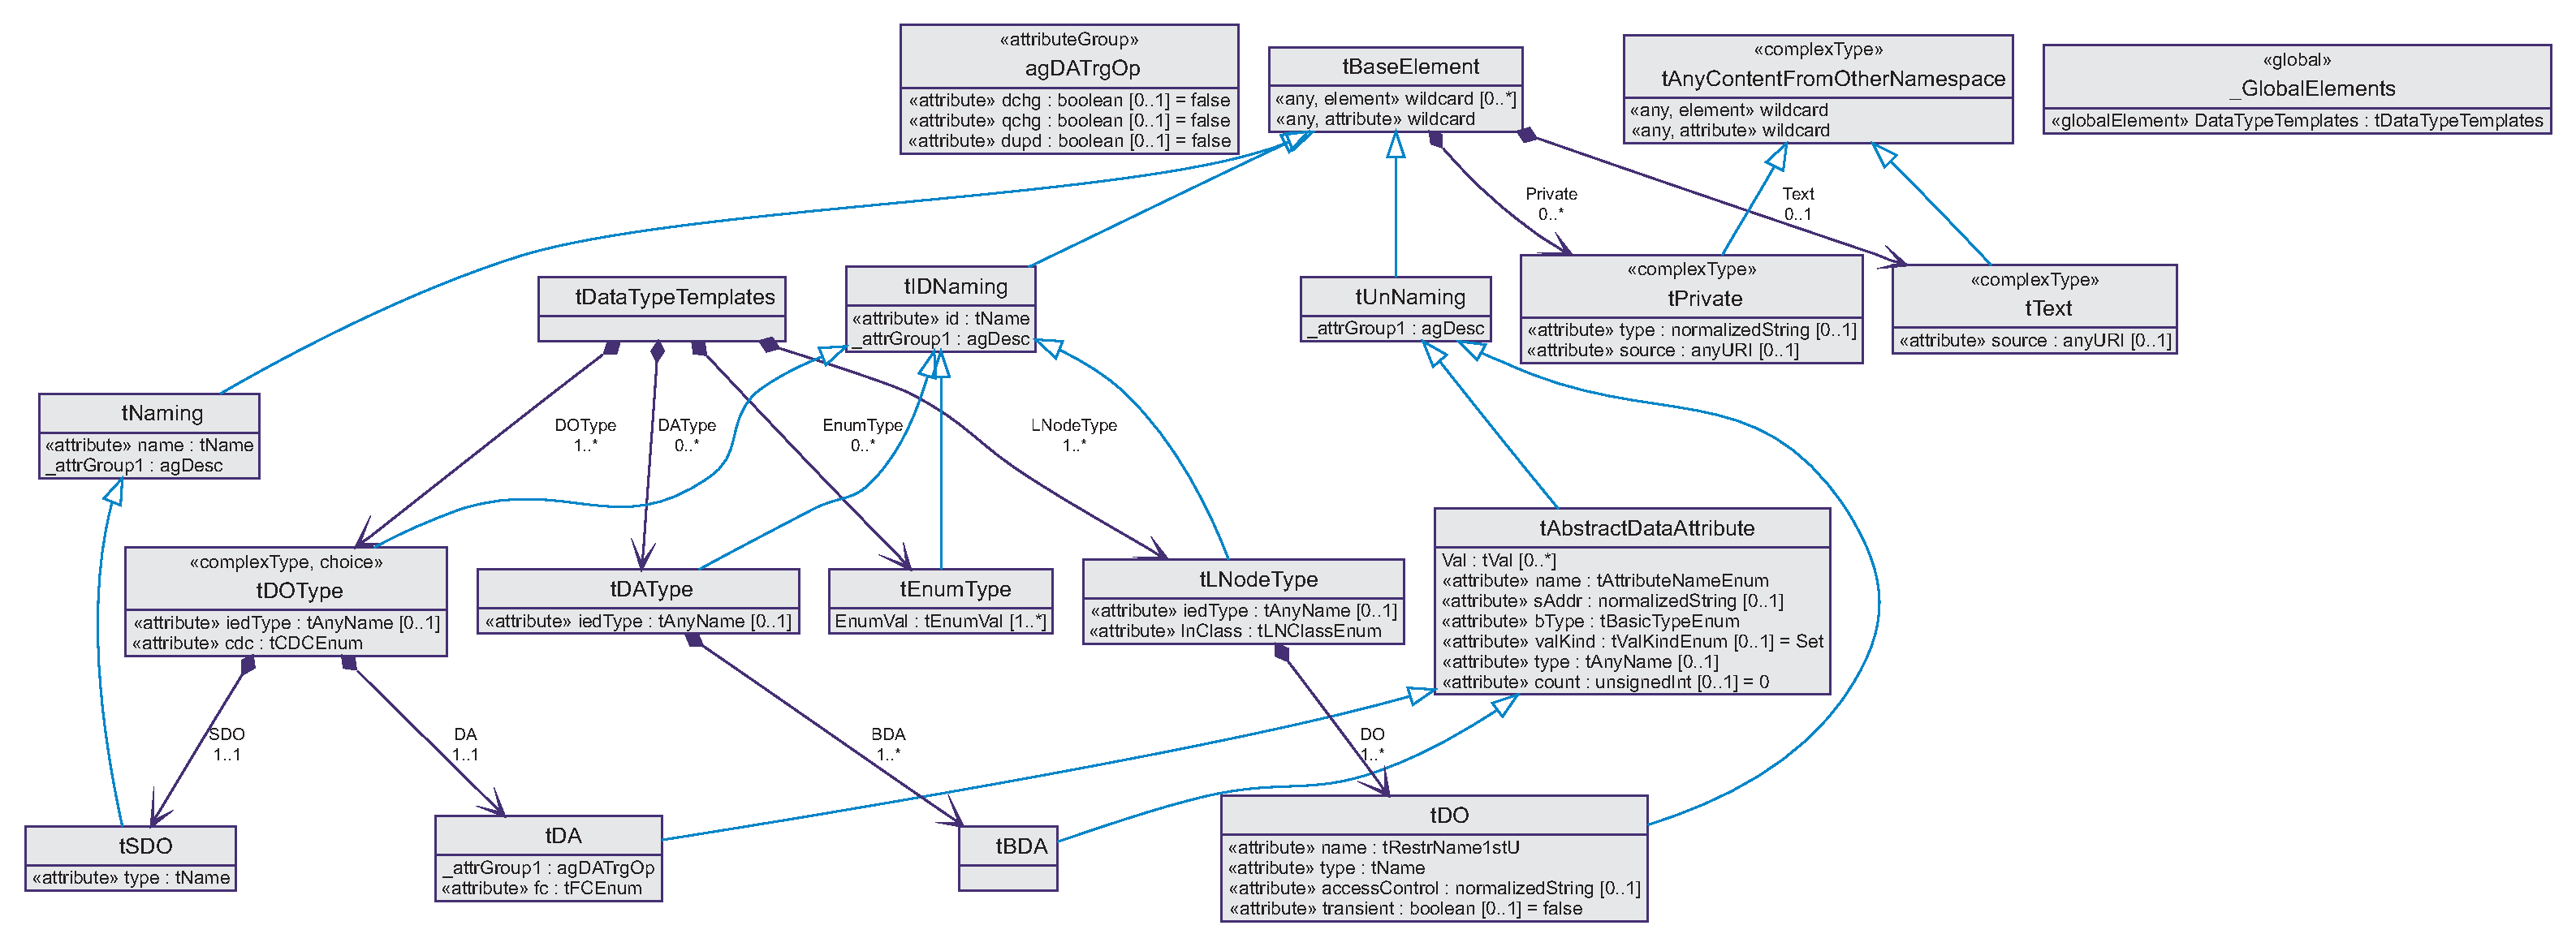
\includegraphics[width=1.0\linewidth]{chapters/enfoque/figures/scl-DataTypeTemplates-depthMax-conHerencia.eps} 
  \captionsetup{font=scriptsize}
  \caption{Clases del elemento \emph{DataTypeTemplate} del SCL, incluyendo
  sus clases abstractas}
  \label{fig:SCL-DataTypeTemplates-depthMax-conHerencia}
\end{center}
\end{figure}
\end{landscape}


\begin{landscape}
\thispagestyle{empty}
\begin{figure}
\begin{center}
  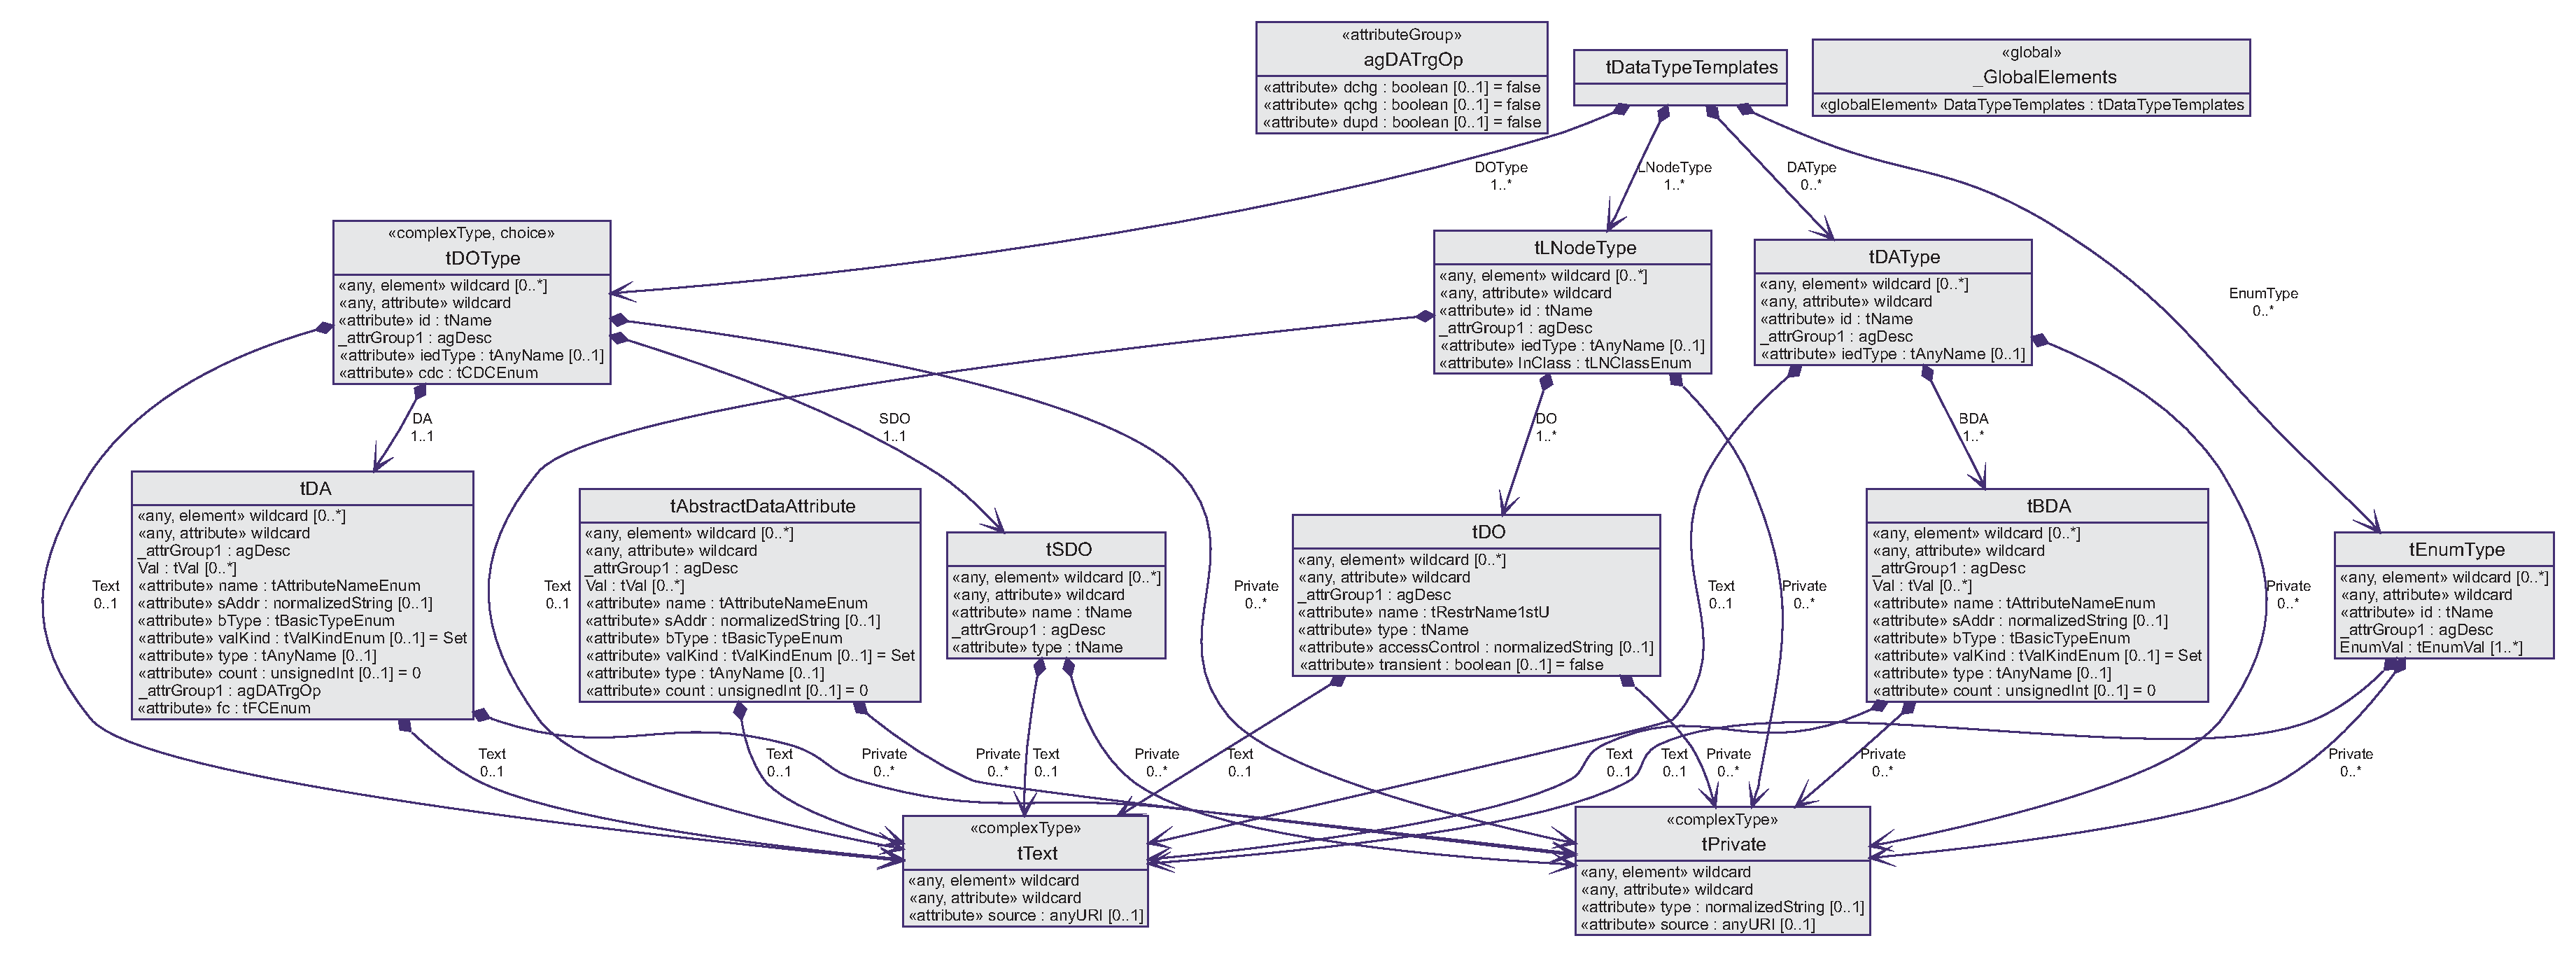
\includegraphics[width=1.0\linewidth]{chapters/enfoque/figures/scl-DataTypeTemplates-depthMax-heredado.eps} 
  \captionsetup{font=scriptsize}
  \caption{Clases del elemento \emph{DataTypeTemplate}
  del SCL, omitiendo sus clases abstractas}
  \label{fig:SCL-DataTypeTemplates-depthMax-heredado}
\end{center}
\end{figure}
\end{landscape}


Seg�n las directrices del EPRI \cite{Epri:2004}, 
uno de los primeros pasos del proceso de ingenier�a 
para la 
especificaci�n de sistemas de 
automatizaci�n de subestaciones usando la norma IEC 61850
consiste en identificar los datos
disponibles, y en base a estos datos, determinar 
los nodos l�gicos correspondientes.

El autor de este trabajo realiz� este paso 
escribiendo en el elemento \textbf{DataTypeTemplate}
de un s�lo archivo SCL todos los nodos l�gicos 
seg�n los datos identificados del sistema. 
En este paso, a�n no se ubican los nodos l�gicos
en los dispositivos l�gicos ni f�sicos. 



\section{Substation}


El modelo de la subestaci�n especificado 
en el elemento SCL \emph{Substation} 
permite construir el modelo de objetos 
de los equipamientos primarios del 
sistema, con las designaciones 
de los puntos de comunicaci�n del sistema
(y la norma IEC 61850 sugiere utilizar 
la norma IEC 61346 \cite{IEC61346-1:1996}
para la nomenclatura de dichos puntos).

Del paradigma \gls{O-O-es} sabemos 
que los objetos IEC 61850 son 
agrupaciones de datos y operaciones con 
memoria aut�noma que podr�a incidir  
en el comportamiento de 
cada invocaci�n.
Los datos de los objetos tienen 
un estado que recuerdan el efecto 
de cada operaci�n \cite{Wegner:1987},
y, a diferencia de las clases, 
los nodos l�gicos del elemento 
\emph{Substation} son objetos que persisten
en el archivo \gls{SCL} a trav�s del 
mecanismo de \glsentryfirst{SO}, 
y los nodos l�gicos implementados en 
los dispositivos IED son objetos IEC 61850
propiamente dichos, 
y s�lo existen en un proceso 
en ejecuci�n. 

 
Centr�ndonos en la interrelaci�n 
entre el modelo de datos 
definidos en el elemento \textbf{IED}
y sus respectivos \textbf{DataTypeTemplates},
podemos afirmar que:
un objeto es creado a partir 
de una clase, en otras palabras, 
un objeto es una instancia de una clase.
An�logamente, los nodos l�gicos de 
los elementos \textbf{IED} 
son creados a partir 
de \textbf{DataTypeTemplates}, 
y siendo m�s espec�fico, los  
elementos \textbf{LN} 
(ver figura \ref{fig:SCL-IED-depthMax-heredado})
son creados a partir de la
plantilla de datos \textbf{LNodeType}
(ver figura \ref{fig:SCL-DataTypeTemplates-depthMax-heredado-simplificado}).


Para fines pr�cticos, se presenta el 
diagrama \gls{UML-es} de las clases 
instanciables del elemento \emph{Substation}
en la figura \ref{fig:SCL-substation-heredado}.
En este diagrama es posible observar 
las restricciones de cantidades 
m�nima y m�xima de instancias permitidas
y su ubicaci�n dentro de la estructura
de la subestaci�n. Como puede observarse 
en el peque�o bosquejo (el diagrama UML
del elemento \emph{Substation} y las 
flechas punteadas en rojo) dise�ado 
sobre el plano de una futura subestaci�n 
paraguaya \cite{Itaipu:6693DE15204E1R0} 
(figura \ref{fig:SCL-SCD-unifilar-villa-hayes}), 
el elemento \emph{Substation} del \gls{SCL} 
permite describir pr�cticamente toda la 
topolog�a de una subestaci�n, 
siendo posible ubicar los nodos l�gicos
en cuaquier nivel jer�rquico del 
diagrama unifilar, gracias a que 
pr�cticamente todas las clases 
instanciables heredan la clase 
abstracta \emph{PowerSystemResource}, 
que hereda de \emph{LNodeContainer} 
las agregaciones de
\emph{LNode} (ver 
figura \ref{fig:SCL-header-conHerencia}).
Para una visi�n totalmente detallada de 
la estructura del elemento subestaci�n
el autor recomienda leer el c�digo \gls{XML}  
\ref{cod:substation-profundo-xml} del 
ap�ndice \ref{app:codigos-SCL}.

\begin{landscape}
\thispagestyle{empty}
\begin{figure}
\begin{center}
  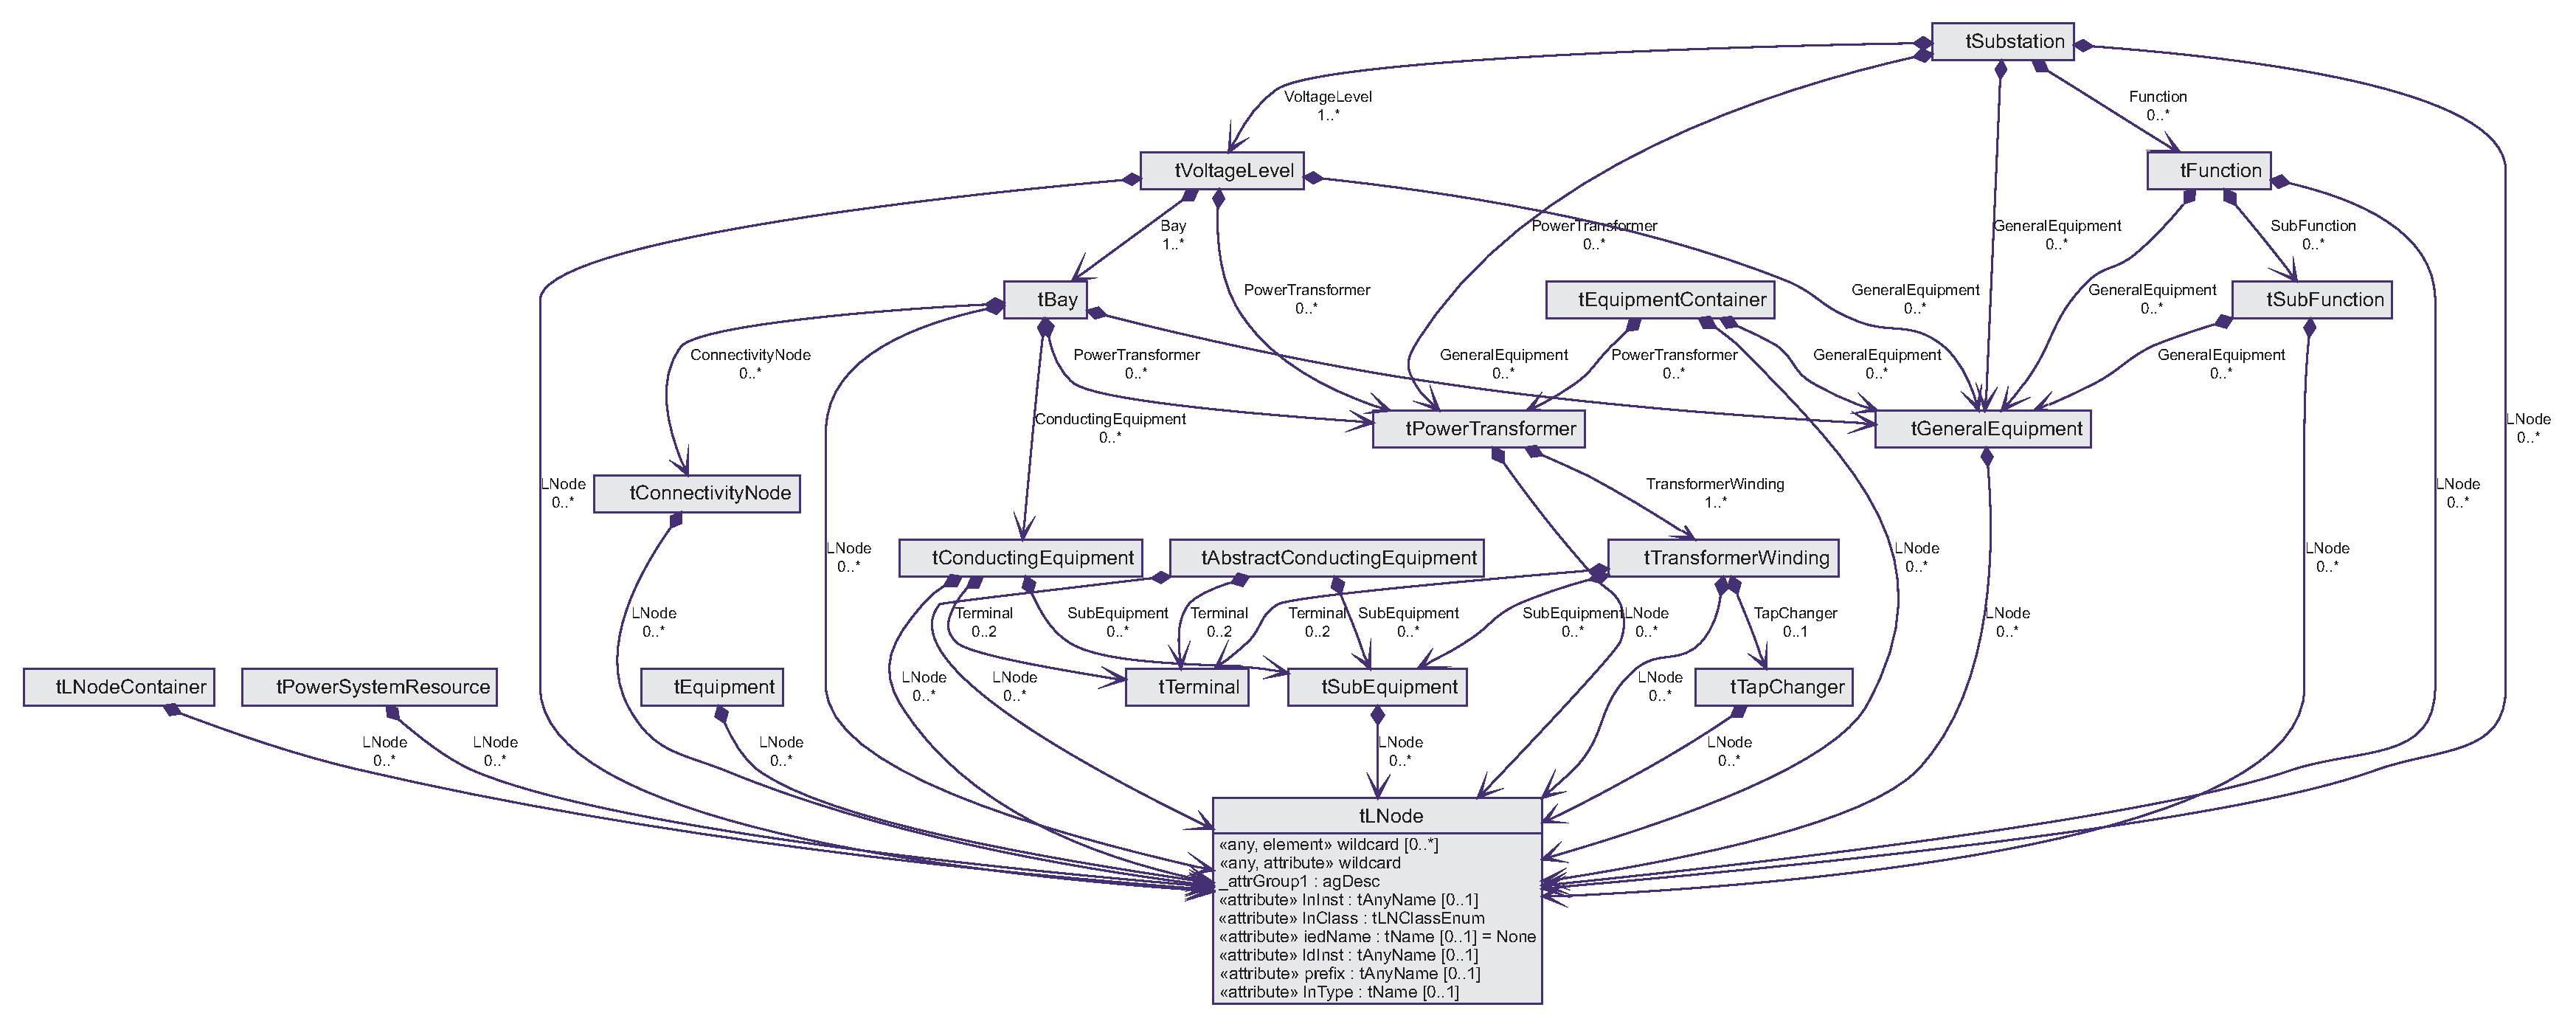
\includegraphics[width=1.0\linewidth]{chapters/enfoque/figures/scl-Substation-dept3-heredado.eps}
  \captionsetup{font=scriptsize}
  \caption{Clases instanciables del elemento \emph{Substation}}
  \label{fig:SCL-substation-heredado}
\end{center}
\end{figure}
\end{landscape}

\begin{landscape}
\thispagestyle{empty}
\begin{figure}
\begin{center}
  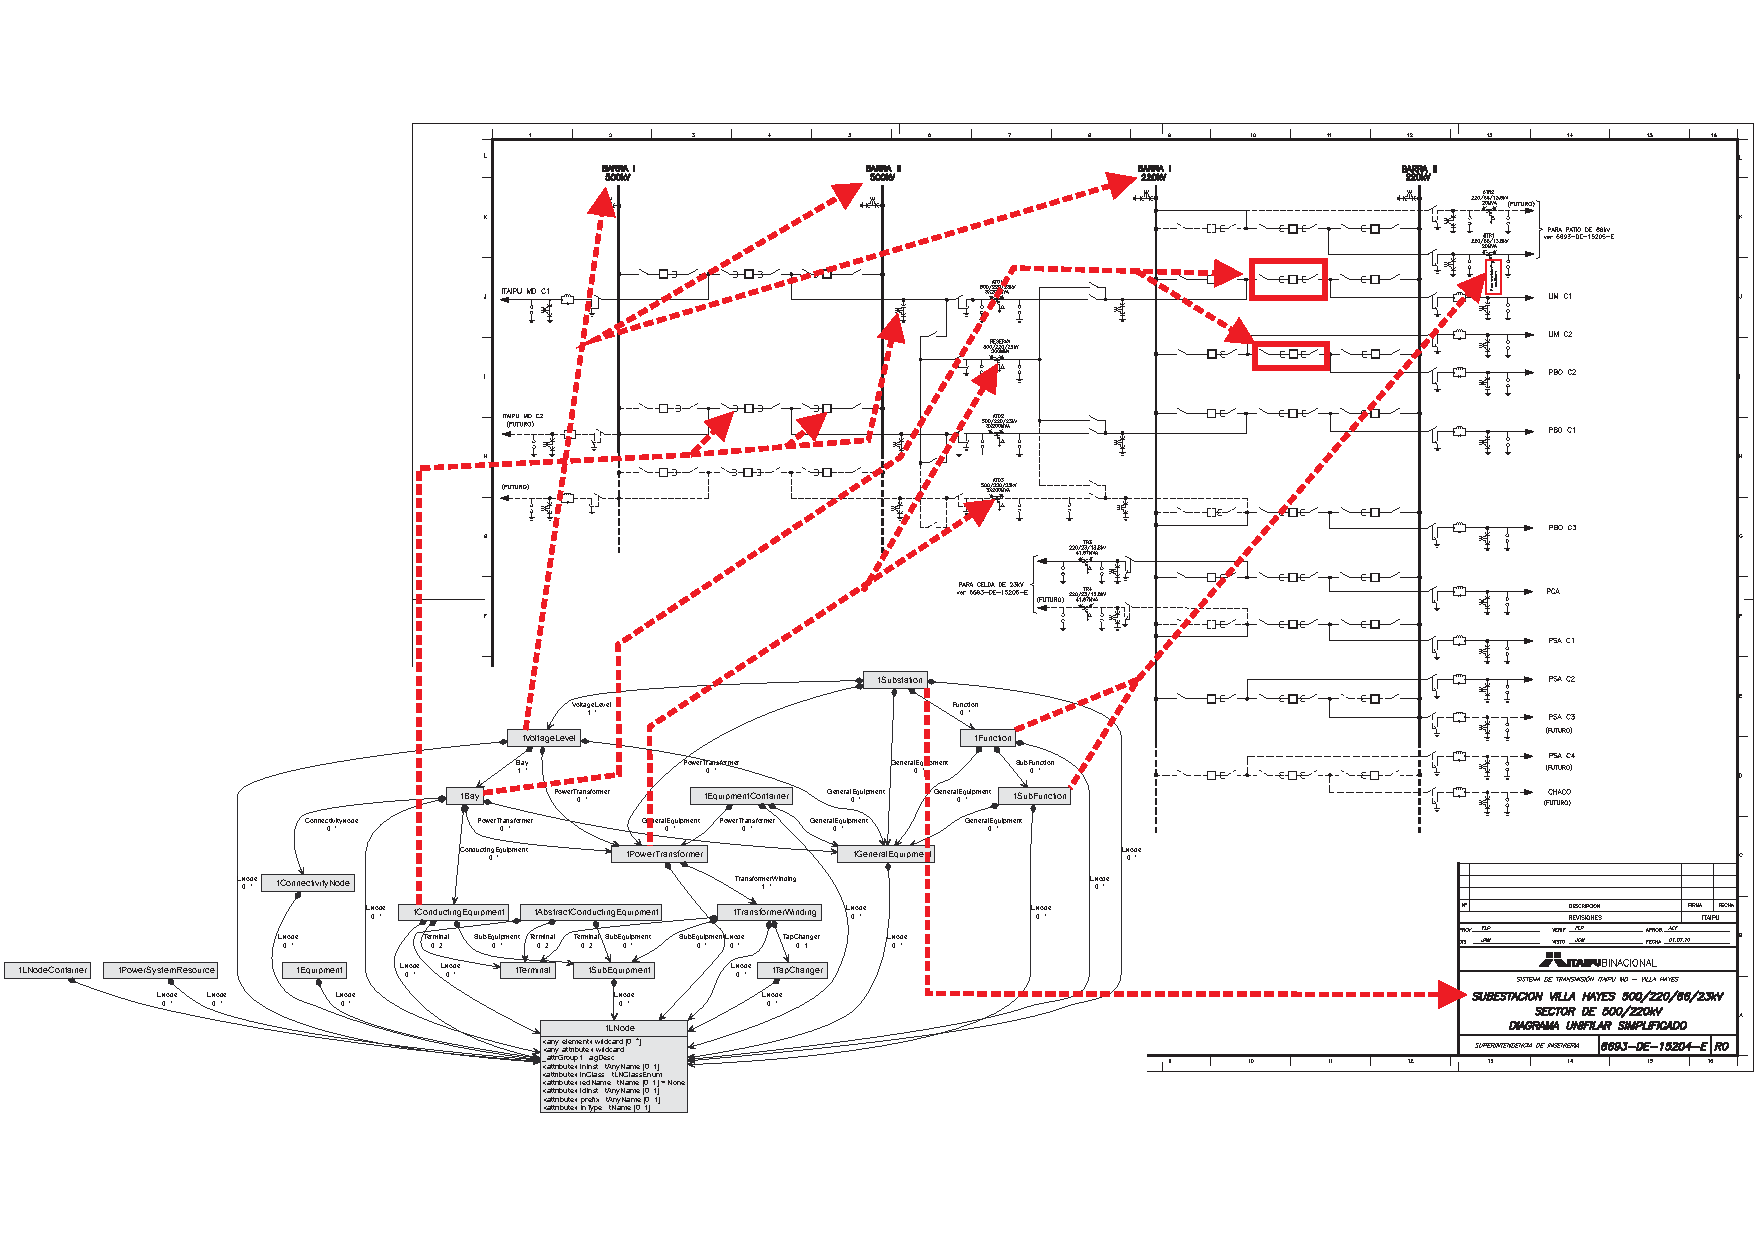
\includegraphics[width=1.0\linewidth]{chapters/enfoque/figures/SSD-and-6693DE15204E1R0} 
  \captionsetup{font=scriptsize}
  \caption{Diagrama unifilar de la subestaci�n Villa Hayes
  \cite{Itaipu:6693DE15204E1R0} y su relaci�n (descripta en forma simplificada) 
  con el SCL.} 
  \label{fig:SCL-SCD-unifilar-villa-hayes}
\end{center}
\end{figure}
\end{landscape}
 
 
 
\begin{landscape}
\thispagestyle{empty}
\begin{figure}
\begin{center}
  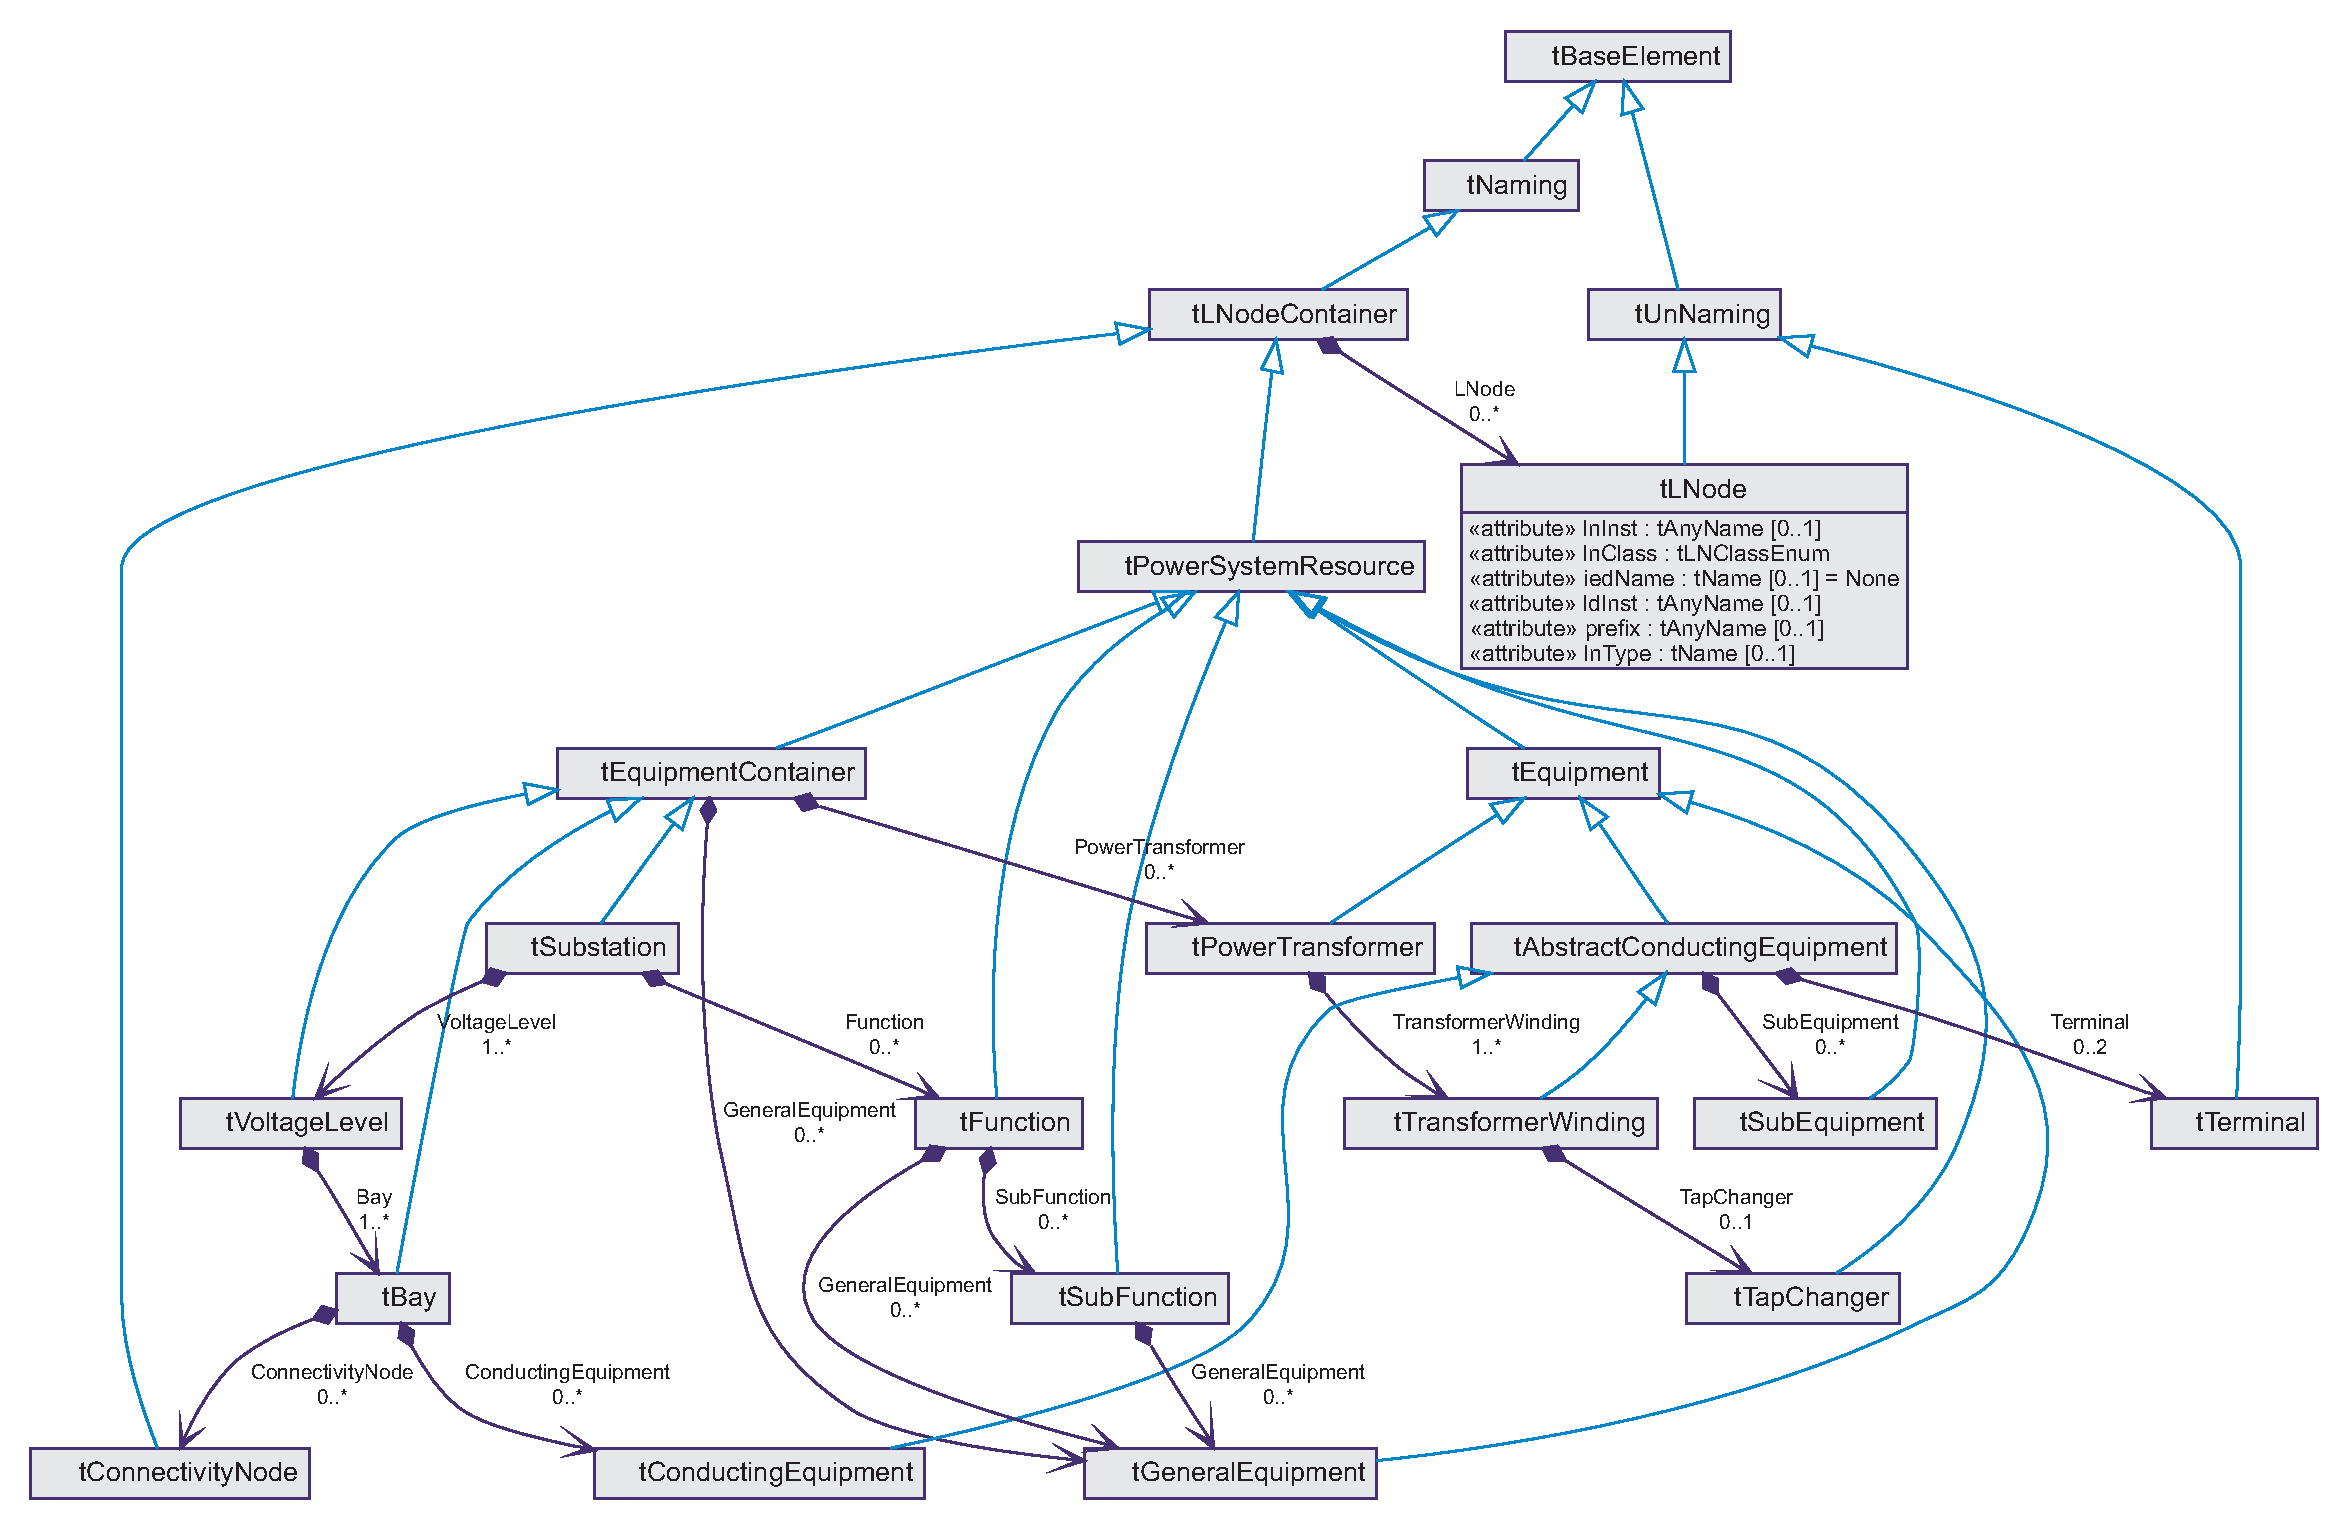
\includegraphics[width=1.0\linewidth]{chapters/enfoque/figures/scl-Substation-deptMax-conHerencia.eps} 
  \captionsetup{font=scriptsize}
  \caption{Clases del elemento \emph{Substation}, incluyendo sus clases abstractas}
  \label{fig:SCL-header-conHerencia}
\end{center}
\end{figure}
\end{landscape}



A pesar de que la variante SSD describe con gran detalle la estructura de las
subestaciones, esta no describe con suficiente detalle 
la estructura de las hidroel�ctricas, es por ello que 
su relevancia en el proceso de ingenier�a en el �mbito de las centrales
hidroel�ctricas debe ser revisado. 
En las subestaciones se define la estructura b�sica en base a niveles de 
voltaje, bay, equipamientos conductores y sus terminales (que est�n 
incluidos en el elemento \emph{Substation}). Actualmente a�n 
no es posible describir la estructura de una hidroel�ctrica, 
usando el SSD, 
en t�rminos de cotas, unidades generadoras y embalses, por ejemplo.  
El SSD provee
una descripci�n sem�ntica de estructura del sistema y es �til 
principalmente para el proyectista (en el �mbito de subestaciones), 
pues gracias a el es posible realizar cambios del sistema 
con mayor facilidad. Este ser�a el uso ideal del SSD. Gracias 
al uso de un s�lo SSD para todo el sistema, se facilita la 
construcci�n de sistemas a prueba de futuro. Sin embargo, 
no siempre es ventajoso empezar el proyecto 
creando el SSD del sistema, ese es s�lo un enfoque entre los
tantos existentes (algunos enfoques se describen en la 
secci�n \ref{sec:ENFOQUE-estado-del-arte-herramientas}). 
El SSD bien podr�a ser creado en otra etapa del proceso 
de ingenier�a. 

Para el enfoque utilizado en este 
trabajo, se ha creado el SSD al final 
del trabajo. En este caso particular, no proporcionaba 
ventajas significativas el uso del SSD, pues entre 
apoyar el dise�o de los nodos l�gicos en 
la topolog�a del sistema 
y en la arquitectura del sistema de comunicaci�n, 
result� m�s adecuado tomar
los \textbf{LNTypes}
con sos respectivos \textbf{DOType} 
que forman parte del \textbf{DataTypeTemplates} 
creado en el paso anterior,
y a partir de all� 
creando las instancias agrupadas en dispositivos l�gicos, 
ya conociendo de antemano la arquitectura del sistema. Se 
describen mayores detalles al respecto 
en la secci�n \ref{sec:ENFOQUE-ssd-vs-icd}.

 
 


\section{Header}

Como puede observarse en la 
figura \ref{fig:SCL-header-con-herencias}, 
el \gls{SCL} permite guardar un historial 
del proceso de ingenier�a. Seg�n 
estas definiciones, es posible realizar 
un control de versiones bien detallado
de los archivos \gls{SCL} dise�ados durante  
el proceso de ingenier�a. En el atributo
\emph{id} se proporciona un 
identificador �nico  
para versionar las distintas variantes  
\gls{SCL}. 


\begin{figure}
\begin{center}
  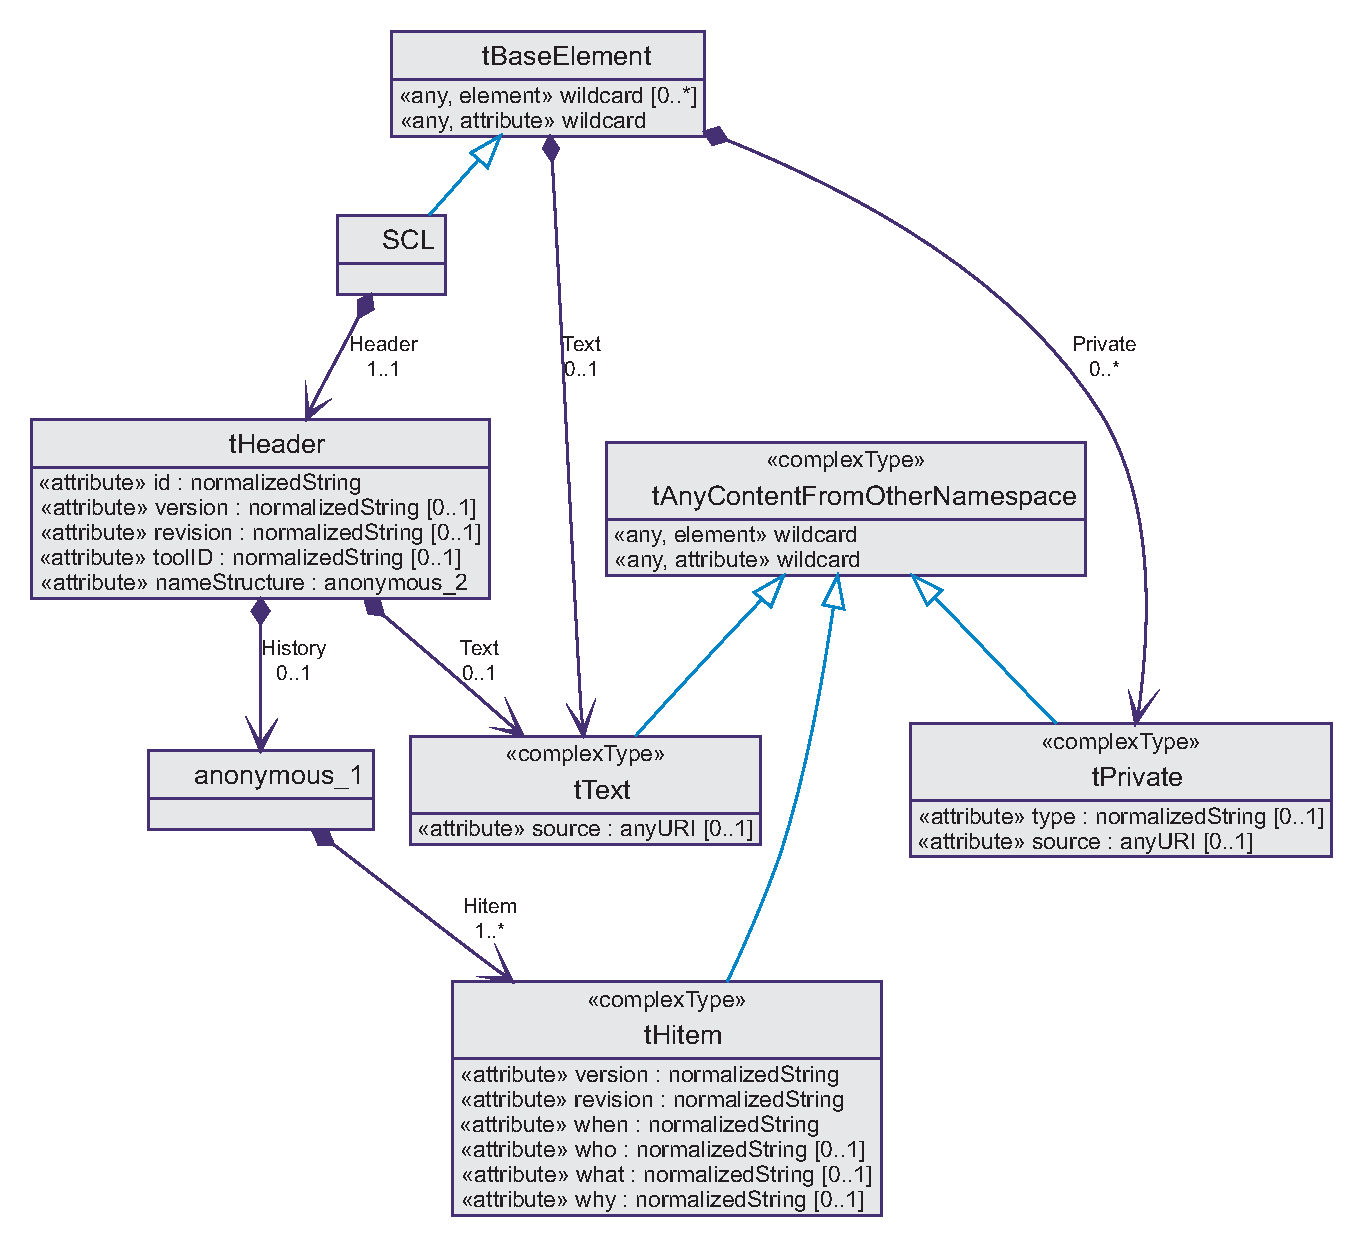
\includegraphics[width=1.0\textwidth]{chapters/enfoque/figures/scl-header-depthMax-conHerencia.eps}
  \caption{\emph{Header} del SCL, incluyendo las herencias
  correspondientes}
  \label{fig:SCL-header-con-herencias}
\end{center}
\end{figure}

El elemento \emph{Header} tambi�n define 
el enfoque del proceso de ingenier�a 
utilizado, pues con su atributo 
\emph{nameStructure} se indica 
si los nombres de se�ales del 
sistema de comunicaci�n proceden del 
elemento \emph{Substation} (generalmente
asociado con el archivo \gls{SSD}) 
o de la estructura de un IED existente 
en el mercado siendo sus posibles valores 
\emph{FuncName} o \emph{IEDName}. 

Con el enfoque utilizado en este trabajo 
se procede a la designaci�n de los nombres 
de las se�ales de comunicaci�n con 
respecto a los IEDs, pero no con IEDs 
procedentes del mercado, sino con 
ICDs dise�ados durante el proceso de ingenier�a
(en la secci�n \ref{chEnfoque:ied-simplif-no-preconfig} se proporciona 
m�s informaci�n sobre el 
enfoque utilizado en el
dise�o de los
modelos de IEDs realizados en este proyecto).

\begin{table}
	\lstinputlisting[label=cod:header-example-xml,
	caption=Ejemplo de Header]
	{chapters/enfoque/source/scl/myHeader.xml} 
\end{table}

Se provee de un trozo de ejemplo del 
ICD correspondiente a un IED a ser 
utilizado en la parte hidr�ulica 
del regualdor de velocidad en 
la lista \ref{cod:header-example-xml}. 
Esta estructura se visualiza mejor 
en el diagrama \gls{UML} 
de la figura \ref{fig:SCL-header-heredado}.  

\begin{figure}
\begin{center}
  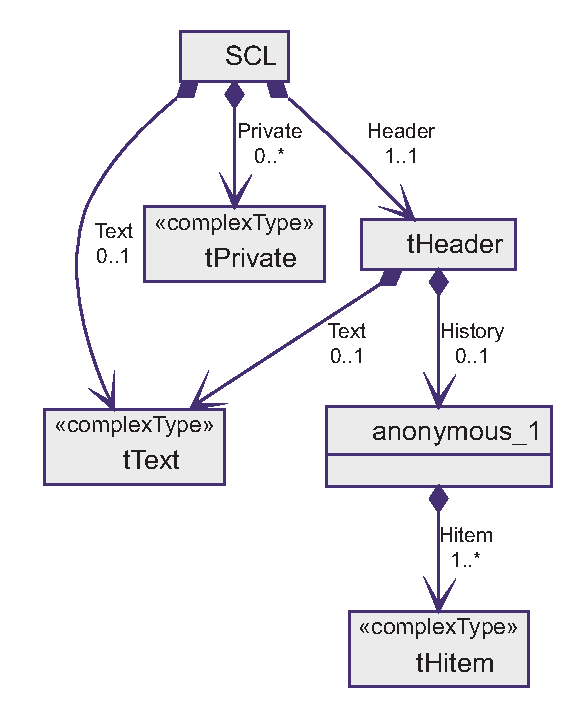
\includegraphics[width=0.4\textwidth]{chapters/enfoque/figures/scl-header-depthMax-heredado.eps}
  \caption{Clases instanciables del \emph{Header}}
  \label{fig:SCL-header-heredado}
\end{center}
\end{figure}






%%\section{IED}



%\section{Communication}
\todo[inline]{ver que hacer con esta seccion} %este voy a deber nom�s, no hay tiempo!
%%\section{AAA}






%\todo[inline]{En este cap�tulo voy a agregar 
%los graficos a continuacion:

%(los ejemplos que voy usando son con estas clases)}


%\begin{figure}
% 
% 
% 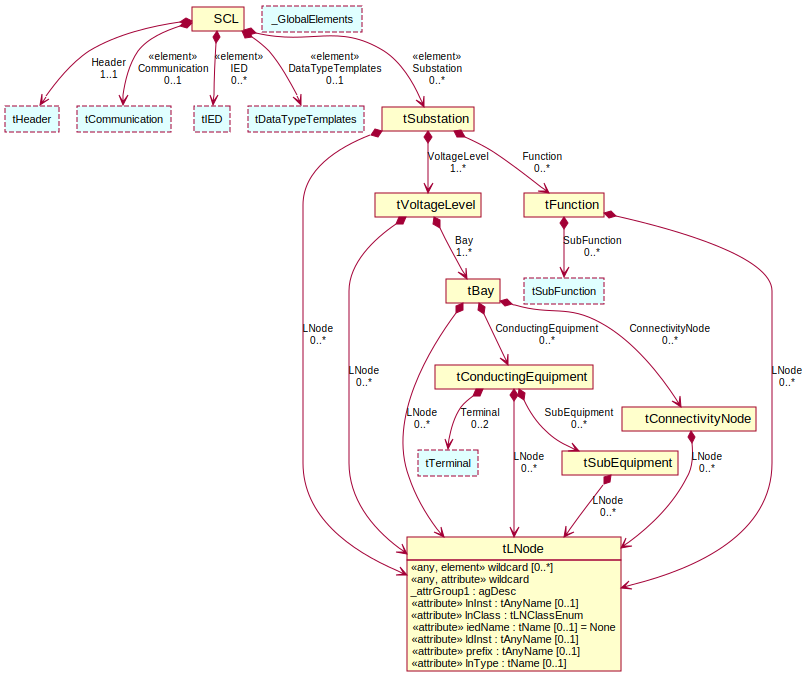
\includegraphics[width=1.0\textwidth]{chapters/oop/figures/LogicalNodeAllocationStructure}
% \caption{Logical Node and their role at the substation level}
% \label{fig:LogicalNodeAllocationStructure}
%\end{figure}

%\begin{landscape}
%	\begin{figure}	
%  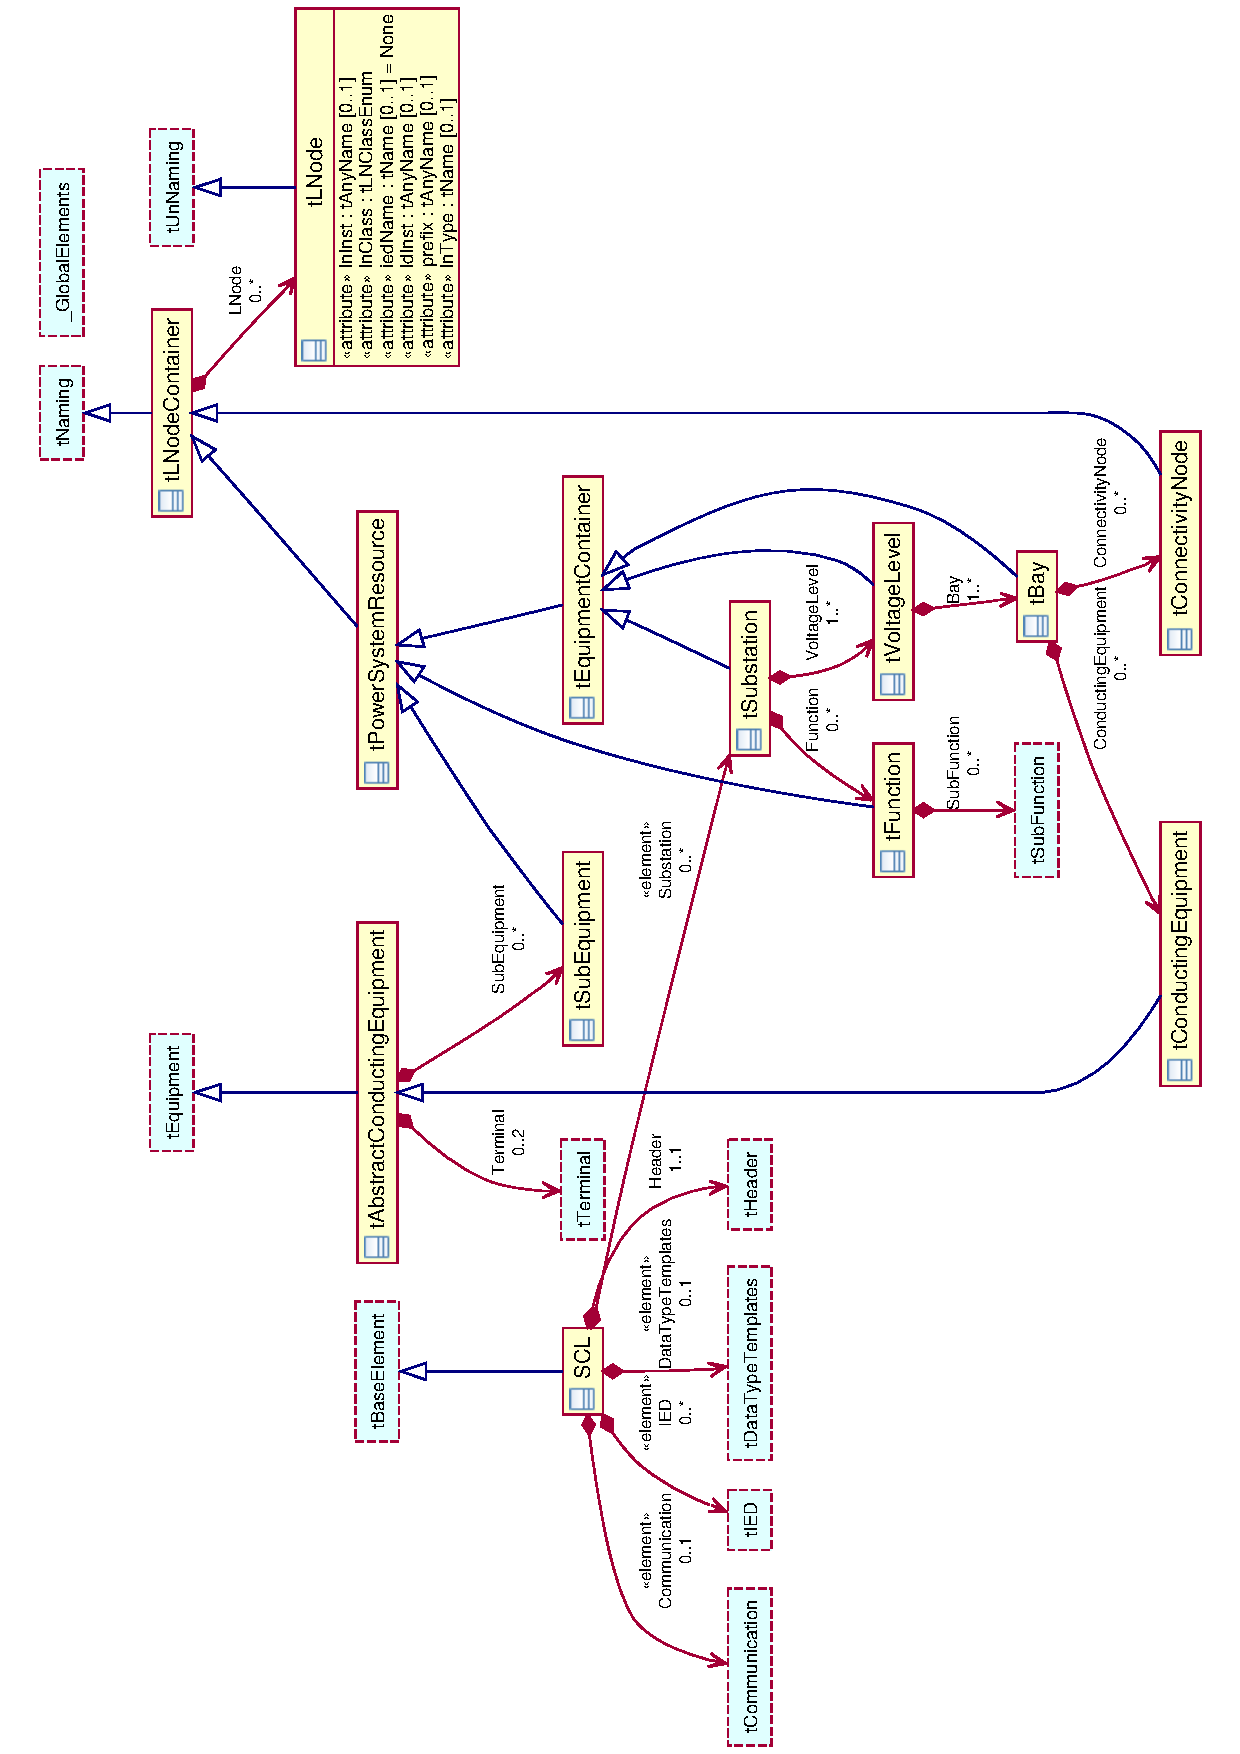
\includegraphics[angle=-90, width=1.0\linewidth]{chapters/oop/figures/LogicalNodeAllocationStructure_with_heritance}
%  \caption{Logical Node and their role at the substation level, depicted with
%  the heritance details}
%  \label{fig:LogicalNodeAllocationStructure_with_heritance}
%\end{figure}
%\end{landscape}
	
%\section{Proceso de ingenier�a IEC 61850 SCL-c�ntrico}


El proceso de ingenier�a 
\section{Especificaci�n de nodos l�gicos en variantes SSD vs. especificaci�n
con variantes ICD}
	\label{sec:ENFOQUE-ssd-vs-icd}
	
	
Seg�n las definiciones de la norma 
IEC 61850--6 \cite{IEC61850-6:2004}, 
la variante SSD puede ser utilizada 
para definir el diagrama unifilar y 
los nodos l�gicos requeridos en dicho
diagrama. 

Seg�n el XML Shema de la norma \cite{IEC61850-6:2004} que define la estructura del SLC
no es obligatorio definir correctamente 
el atributo \emph{iedName} del 
elemento \emph{LNode} en la variante SSD, debido a esto, 
la especificaci�n de nodos l�gicos de IEDs  (productos)
con la variante SSD puede 
inducir a errores, dado que en un SSD (aunque est� en 
plena conformidad con la norma IEC 61850) 
no valida en forma autom�tica 
la definici�n de ubicaciones de nodos l�gicos 
en los respectivos IEDs y tampoco se provee 
la agrupaci�n en Dispositivos L�gicos sin
antes haber creado el SSD (generalmente
los sistemas se construyen con cientos de instancias 
de nodos l�gicos, por lo que deber�a haber 
una asistencia por parte del software de modo
a minimizar los errores humanos). 
Si las herramientas 
de ingenier�a permitieran forzar la identificaci�n 
de los nodos l�gicos en sus respectivos IEDs
y posibilitaran la visualizaci�n en modo gr�fico 
o con tablas de las agrupaciones de LNodes realizadas 
en archivos SSD 
este problema ser�a resuelto, 
pero como no lo hacen \cite{PTI:SESEP2010}, 
existe una alta probabilidad de que 
algunos nodos l�gicos
no est�n bien ubicados, o directamente  
no est�n ubicados a 
ning�n IED en variantes SSD 
dise�adas para especificaciones t�cnicas 
de IEDs (esto se soluciona utilizando 
gr�ficos hechos en programas tales como AutoCAD, 
pero en este trabajo se busca
un enfoque a trav�s del cual se pueda obtener
un dise�o IEC 61850 totalmente basado en SCL). 

Es por ello que el autor de este trabajo 
ha analizado otras alternativas que asistan  
las especificaciones simplificadas 
y dise�os del modelo de sistema IEC 61850 realizado.
La especificaci�n de nodos l�gicos con la
variante ICD que posea una profundidad de 
descripci�n adecuada y bien definida resuelve 
todos los problemas que se podr�an ocasionar 
al especificar con variantes SSD como producto 
final de la especificaci�n.

El SSD creado al final del trabajo tiene en cuenta
los siguientes v�nculos XML:

\lstinputlisting[label=cod:slc-ssd-ln-constraints,
caption=Reglas definidas en IEC 61850-6 para la construcci�n de nodos l�gicos en
la variante SSD] {chapters/enfoque/source/scl/ssd-ln-constraint.xsd} 

por lo que el resultado del SSD es muy aproximado 
al SCD, dado que ya se realiza el mapeo de los 
\textbf{LN} de ICDs a \textbf{LNodes} del SSD. 

En la siguiente secci�n, el autor describe este
tipo de variante ICD mencionado anteriormente. 
\section{IED simplificado y no pre-configurado}

\label{sec:ied-simplificado-y-no-pre-configurado}


En esta secci�n el autor propone el concepto de 
ISNP (IED simplificado y no pre--configurado).

Se dice que los ICDs est�n pre--configurados cuando 
ya traen desde el TEMPLATE del ICD (la norma IEC 61850 recomienda 
dar el nombre de TEMPLATE al ICD nuevo, obtenido del fabricante y sin cambiar
nada) configuraciones para env�o 
de informaci�n a trav�s de la red
de forma eficiente a trav�s de agrupaciones
adecuadas de datos (\emph{DataSet}, \emph{Report}), o incluso asociaciones
\emph{MCAA} o \emph{TPAA} ya preparadas.  Por dar un ejemplo, la
herramienta de ingenier�a PCM600 de la ABB, trae ICDs pre-configurados que han sido dise�ados para 
usos en funciones de automatizaci�n muy generales
%\footnote{http://www02.abb.com/global/clabb/clabb151.nsf/bf177942f19f4a98c1257148003b7a0a/088b8658171c587bc125732c0058f550/$FILE/1MRK511200-UEN_-_en_PCM_600_engineering_workflow_for_pre-configured_IED_670.pdf}.
%\footnote{\url{http://www02.abb.com/global/clabb/clabb151.nsf/bf177942f19f4a98c1257148003b7a0a/088b8658171c587bc125732c0058f550/$FILE/1MRK511200-UEN_-_en_PCM_600_engineering_workflow_for_pre-configured_IED_670.pdf}}.
\footnote{\url{http://goo.gl/L80ft}}.


El autor define a un ICD como simplificado si el elemento \emph{IED} del 
SCL posee solamente los nodos hijos y sus atributos obligatorios, m�s las  
instancias de los nodos l�gicos y las instancias de los \emph{Data Objects}
pero sin sus nodos hijos, y sin asociaciones ni agrupaciones de datos, pero 
incluyendo obligatoriamente todos los servicios que ser�n utilizados, 
y las referencias a los nodos hijos del \textbf{DataTypeTemplate}
correspondientes solamente a las instancias definidas en el 
elemento IED.
La definici�n de ICD simplificado puede observarse en la figura
\ref{fig:SCL-IED-ISNP-heredado}.

Es ilustrativo comparar la estructura de un ICD ISNP (figura
\ref{fig:SCL-IED-ISNP-heredado}) y el de un ICD completo (figura
\ref{fig:SCL-IED-depthMax-heredado} y 
c�digo fuente \ref{cod:ied-profundo-xml}). 

\begin{landscape}
\thispagestyle{empty}
\begin{figure}
\begin{center}
  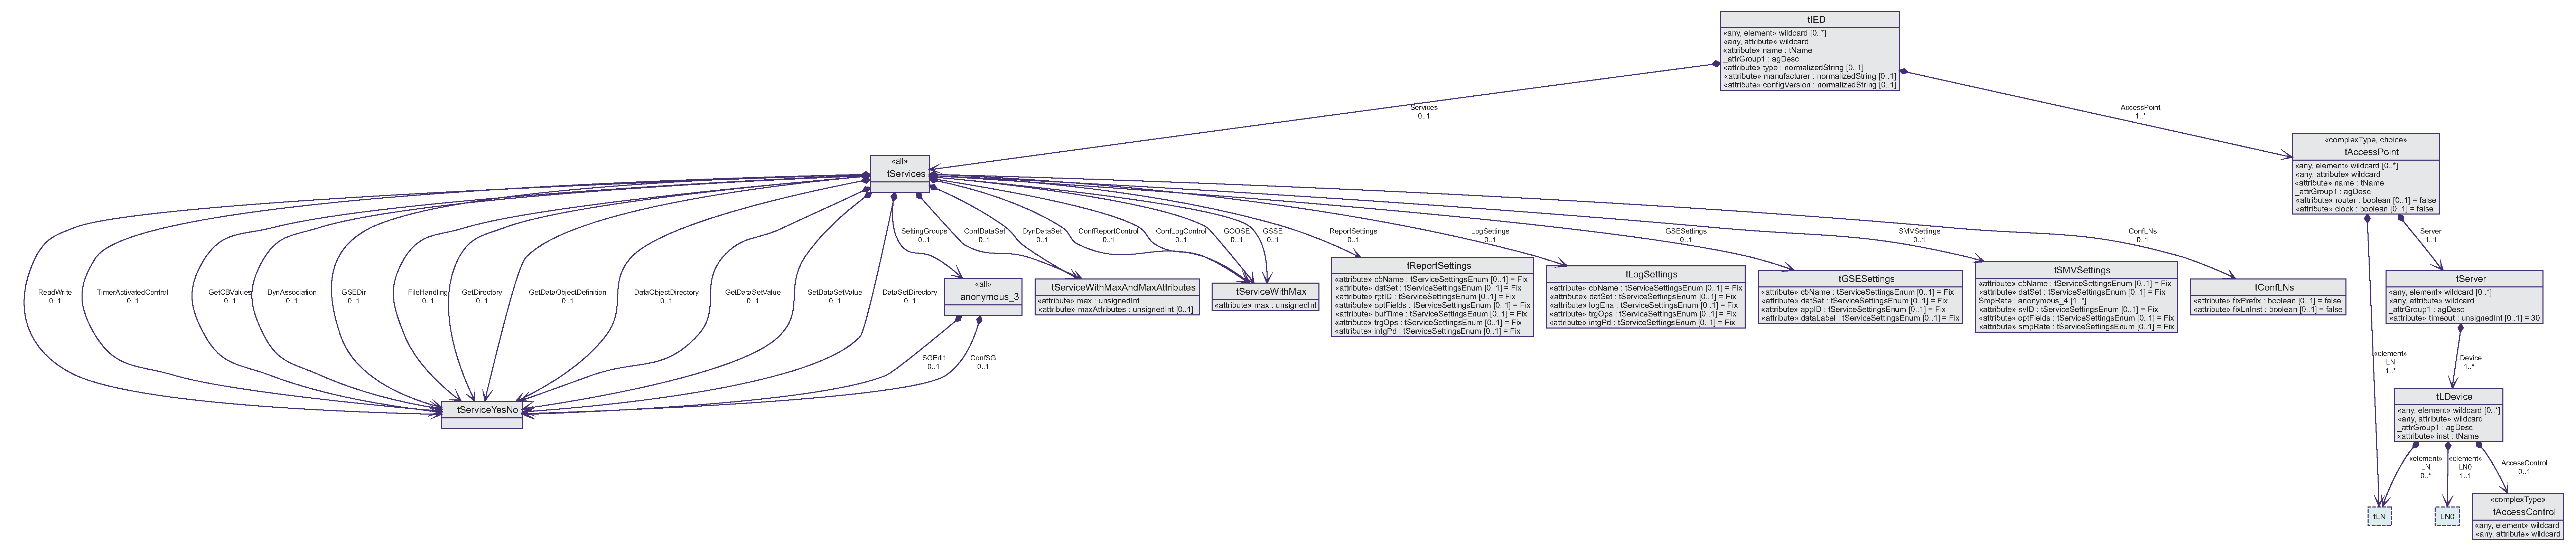
\includegraphics[width=1.0\linewidth]{chapters/enfoque/figures/scl-IED-depthISNP-heredado.eps}
  \captionsetup{font=scriptsize}
  \caption{Diagrama de clases para un IED ISNP}
  \label{fig:SCL-IED-ISNP-heredado}
\end{center}
\end{figure}
\end{landscape}

La construcci�n de ICDs del tipo ISNP permite enfocar de una manera nueva 
la espeficicaci�n t�cnica de IEDs, pues en la variante ICD 
es posible definir los nodos l�gicos a ser utilizados por cada IED, 
agrupados en sus respectivos \emph{Logical Devices}, 
definiendo los \emph{DataObjects} de cada nodo l�gico, 
y describiendo los servicios de comunicaci�n que deber�n utilizarse.
En realidad, al contrario de lo que pueda imaginarse el lector, 
la construcci�n de ICDs del tipo ISNP no es dif�cil ni lleva mucho tiempo, 
pues se describe solamente lo escencial, lo m�nimo que podr�a tener 
un IED. Y lo m�s importante, dicha descripci�n se realiza de una 
manera formal (y en plena conformidad con la norma IEC 61850). En otras
palabras, cualquier fabricante de IEDs podr� entener claramente las necesidades
del sistema IEC 61850 de la planta
sin tener que redactar documentos con largas 
explicaciones sobre los modelos de informaci�n,
modelos de servicios y arquitectura.
En las definiciones formales de 
nodos l�gicos del apartado 
IEC 61850--7--410 \cite{IEC61850-7-410:2007} 
no se definen los servicios de comunicaci�n  
de cada nodo l�gico
(en el apartado IEC 61850--7--4 \cite{IEC61850-7-4:2003}
s� se definen), pero es posible observar los
servicios de comunicaci�n de los \textbf{CDCs}
utilizados. Cabe destacar que, en caso que
se necesiten m�s servicios que los mencionados 
en estos apartados de la norma, ellos 
deben ser bien especificados.

\label{chEnfoque:ied-simplif-no-preconfig}
Con este nuevo enfoque, tambi�n surge un nuevo reto: Elaborar 
una espeficicaci�n de nodos l�gicos y servicios de comunicaci�n 
que el fabricante pueda ofrecer. 
Si bien es m�s sencillo especificar nodos l�gicos, 
la espeficicaci�n t�cnica de las capacidades m�nimas de los servicios de
comunicaci�n de los IEDs que necesita la planta
es un poco m�s complicada, dado que
se puede incurrir a especificar servicios que si bien est�n definidos 
por la norma, no existen en el mercado. 

Es por ello que 
el autor propone la utilizaci�n de base de datos de ICDs 
de m�ltiples fabricantes, y de esa forma obtener datos 
estad�sticos de las capacidades de los ICDs existentes actualmente en el
mercado. Siguiendo este planteamiento, el autor ha elaborado 
un \emph{script} Python a trav�s del cual se obtuvieron las tablas 
del ap�ndice \ref{app:Estadisticas-servicios}, 
donde se observan los servicios de comunicaci�n que 
est�n implementados en 178 ICDs 
de cuatro fabricantes distintos. 
El hecho de que la espeficicaci�n t�cnica de los sistemas 
IEC 61850 definan los servicios m�nimos que deban tener 
los dispositivos (incluyendo la configuraci�n de los atributos de los
servicios) permite dise�ar sistemas realmente a prueba de futuro, 
pues en caso que un equipo se da�e, ser� muy simple sustituirlo 
con otro, aunque sea de otro fabricante, sin tener que cambiar 
el dise�o de parte importante del sistema. Por dar un ejemplo, 
al sustituir un IED con capacidades IEC 61850 distintas 
cambiar�a el 
dise�o del modelo IEC 61850 de todo un bay, lo cual a la vez
provocar�a desuniformidad de modelos con respecto 
a los dem�s bays (que en teor�a deber�an ser iguales), y 
de esa forma el sistema se vuelve complejo innecesariamente. 
Los atributos de los servicios definidos en SCL 
tambi�n son importantes, pues, volviendo al mismo escenario del 
ejemplo del bay con un IED a ser cambiado, 
si el IED a ser retirado utilizaba un \emph{DataSet}
con 150 atributos de datos instanciados, y el nuevo 
IED permite como m�ximo el env�o de 50 atributos de 
datos instanciados, entonces se deber� rever parte 
importante del proyecto\footnote{Interoperability and Replacement of an IED by another
one \url{http://blog.iec61850.com/2010/09/interoperability-and-replacement-of-ied.html}}. En
este caso se puede observar que la espeficicaci�n t�cnica de servicios de comunicaci�n ayuda a 
construir sistemas donde la intercambiabilidad de equipos 
sea m�s sencilla. En este caso tambi�n resulta �til 
utilizar m�todos estad�sticos aprovechando la 
base de datos de ICDs, para conocer hasta cu�ntos
atributos de datos instanciados se pueden agrupar en cada \emph{DataSet}
seg�n las capacidades de los fabricantes y el estado 
del arte de las tecnolog�as IEC 61850. 
 
La selecci�n apropiada de los nodos l�gicos 
y de los \textbf{Data Objects}
permite al due�o de la planta asegurar que los nodos l�gicos 
cumplan con los requerimientos funcionales. 
La definici�n del tipo del nodo l�gico
y su cantidad de instancias no siempre es 
suficiente. En el presente trabajo se observa la necesidad de 
especificar
los \textbf{DOType} y \textbf{DOI} en el \textbf{SCL}. 
Dando un ejemplo este enfoque queda m�s claro: si en la
hidroel�ctrica se necesita medir la frecuencia el�ctrica, 
se definir�a el nodo l�gico \textbf{MMXU},
pero como el nodo l�gico de tipo \textbf{MMXU} tiene 
como \textbf{Data} opcional a la frecuencia,
si el IED en realidad no implementa el \textbf{Data Object} \emph{Hz},
el nodo l�gico no estar� cumpliendo con los requisitos
funcionales existentes en la planta, por lo que 
resulta pertinente especificar el nodo l�gico
\textbf{MMXU} y por lo menos su \textbf{DO} \emph{Hz}.


\begin{landscape}
\thispagestyle{empty}
\begin{figure}
\begin{center}
  %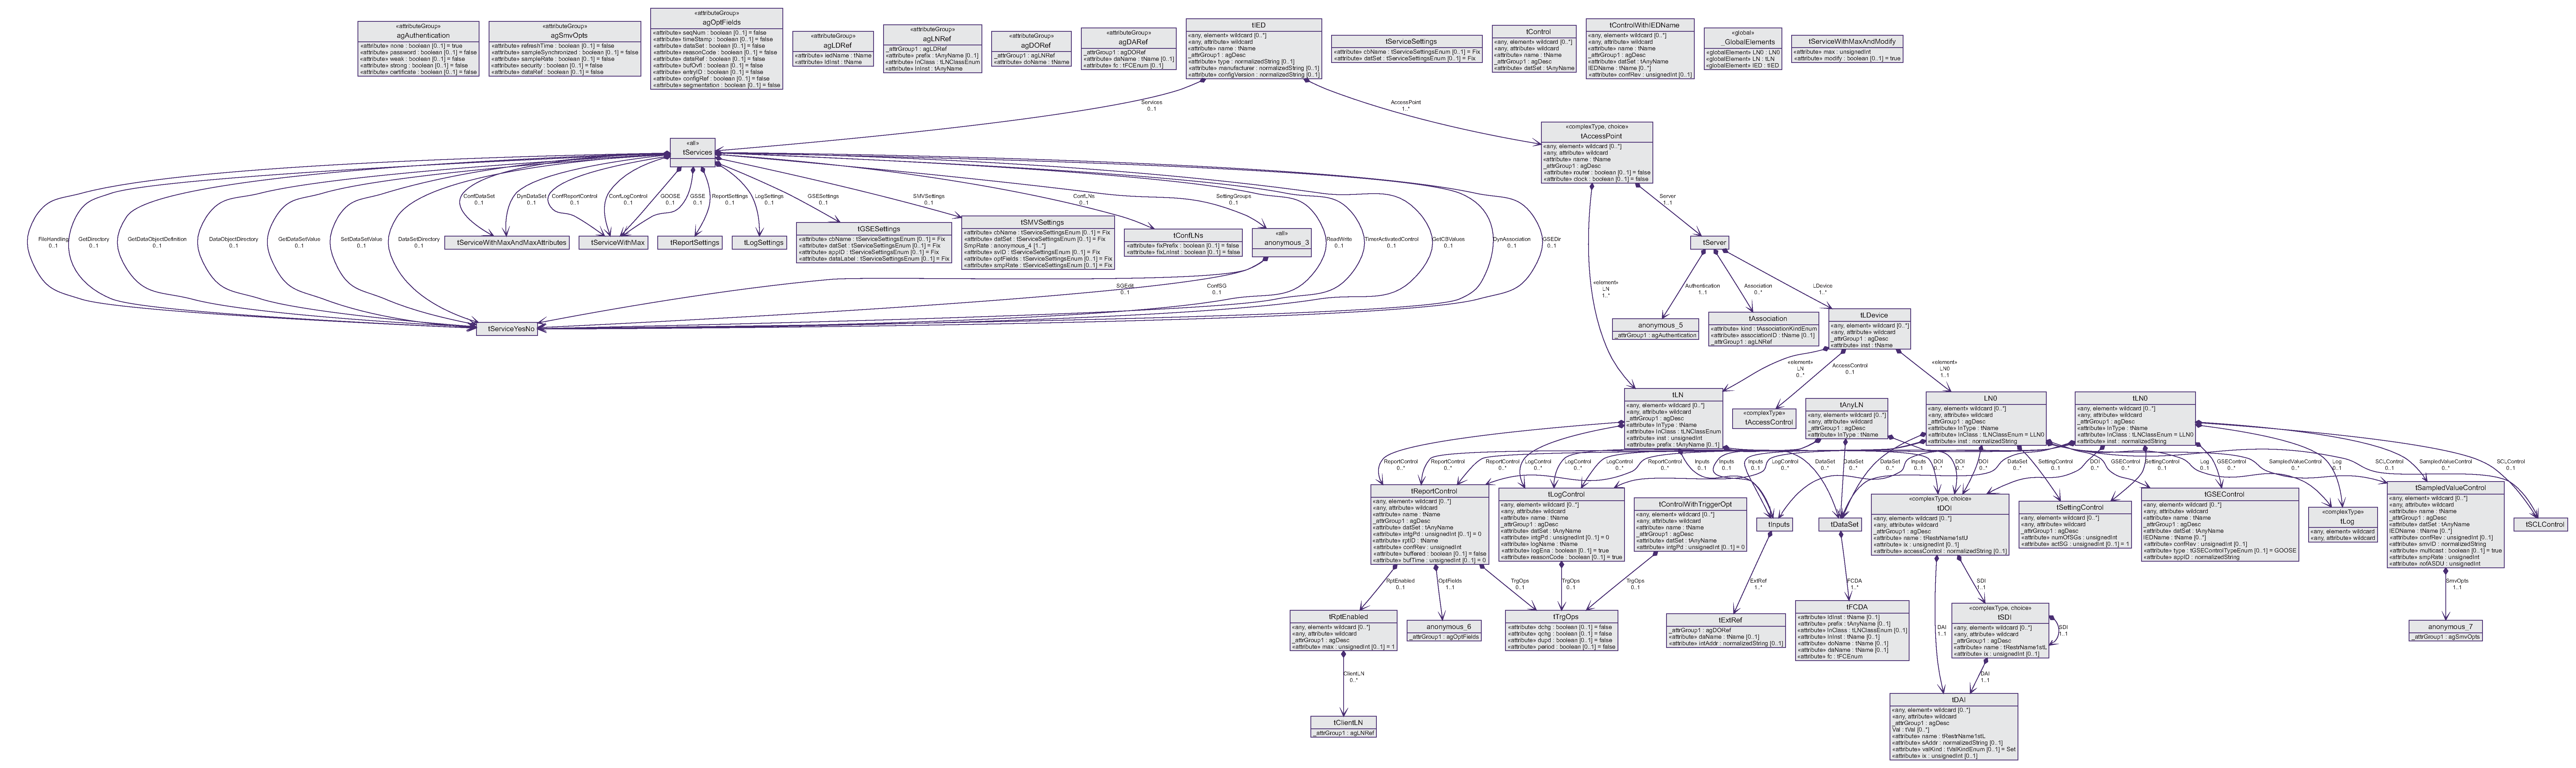
\includegraphics[width=1.0\linewidth]{chapters/enfoque/figures/scl-IED-depthMax-heredado.eps} 
  %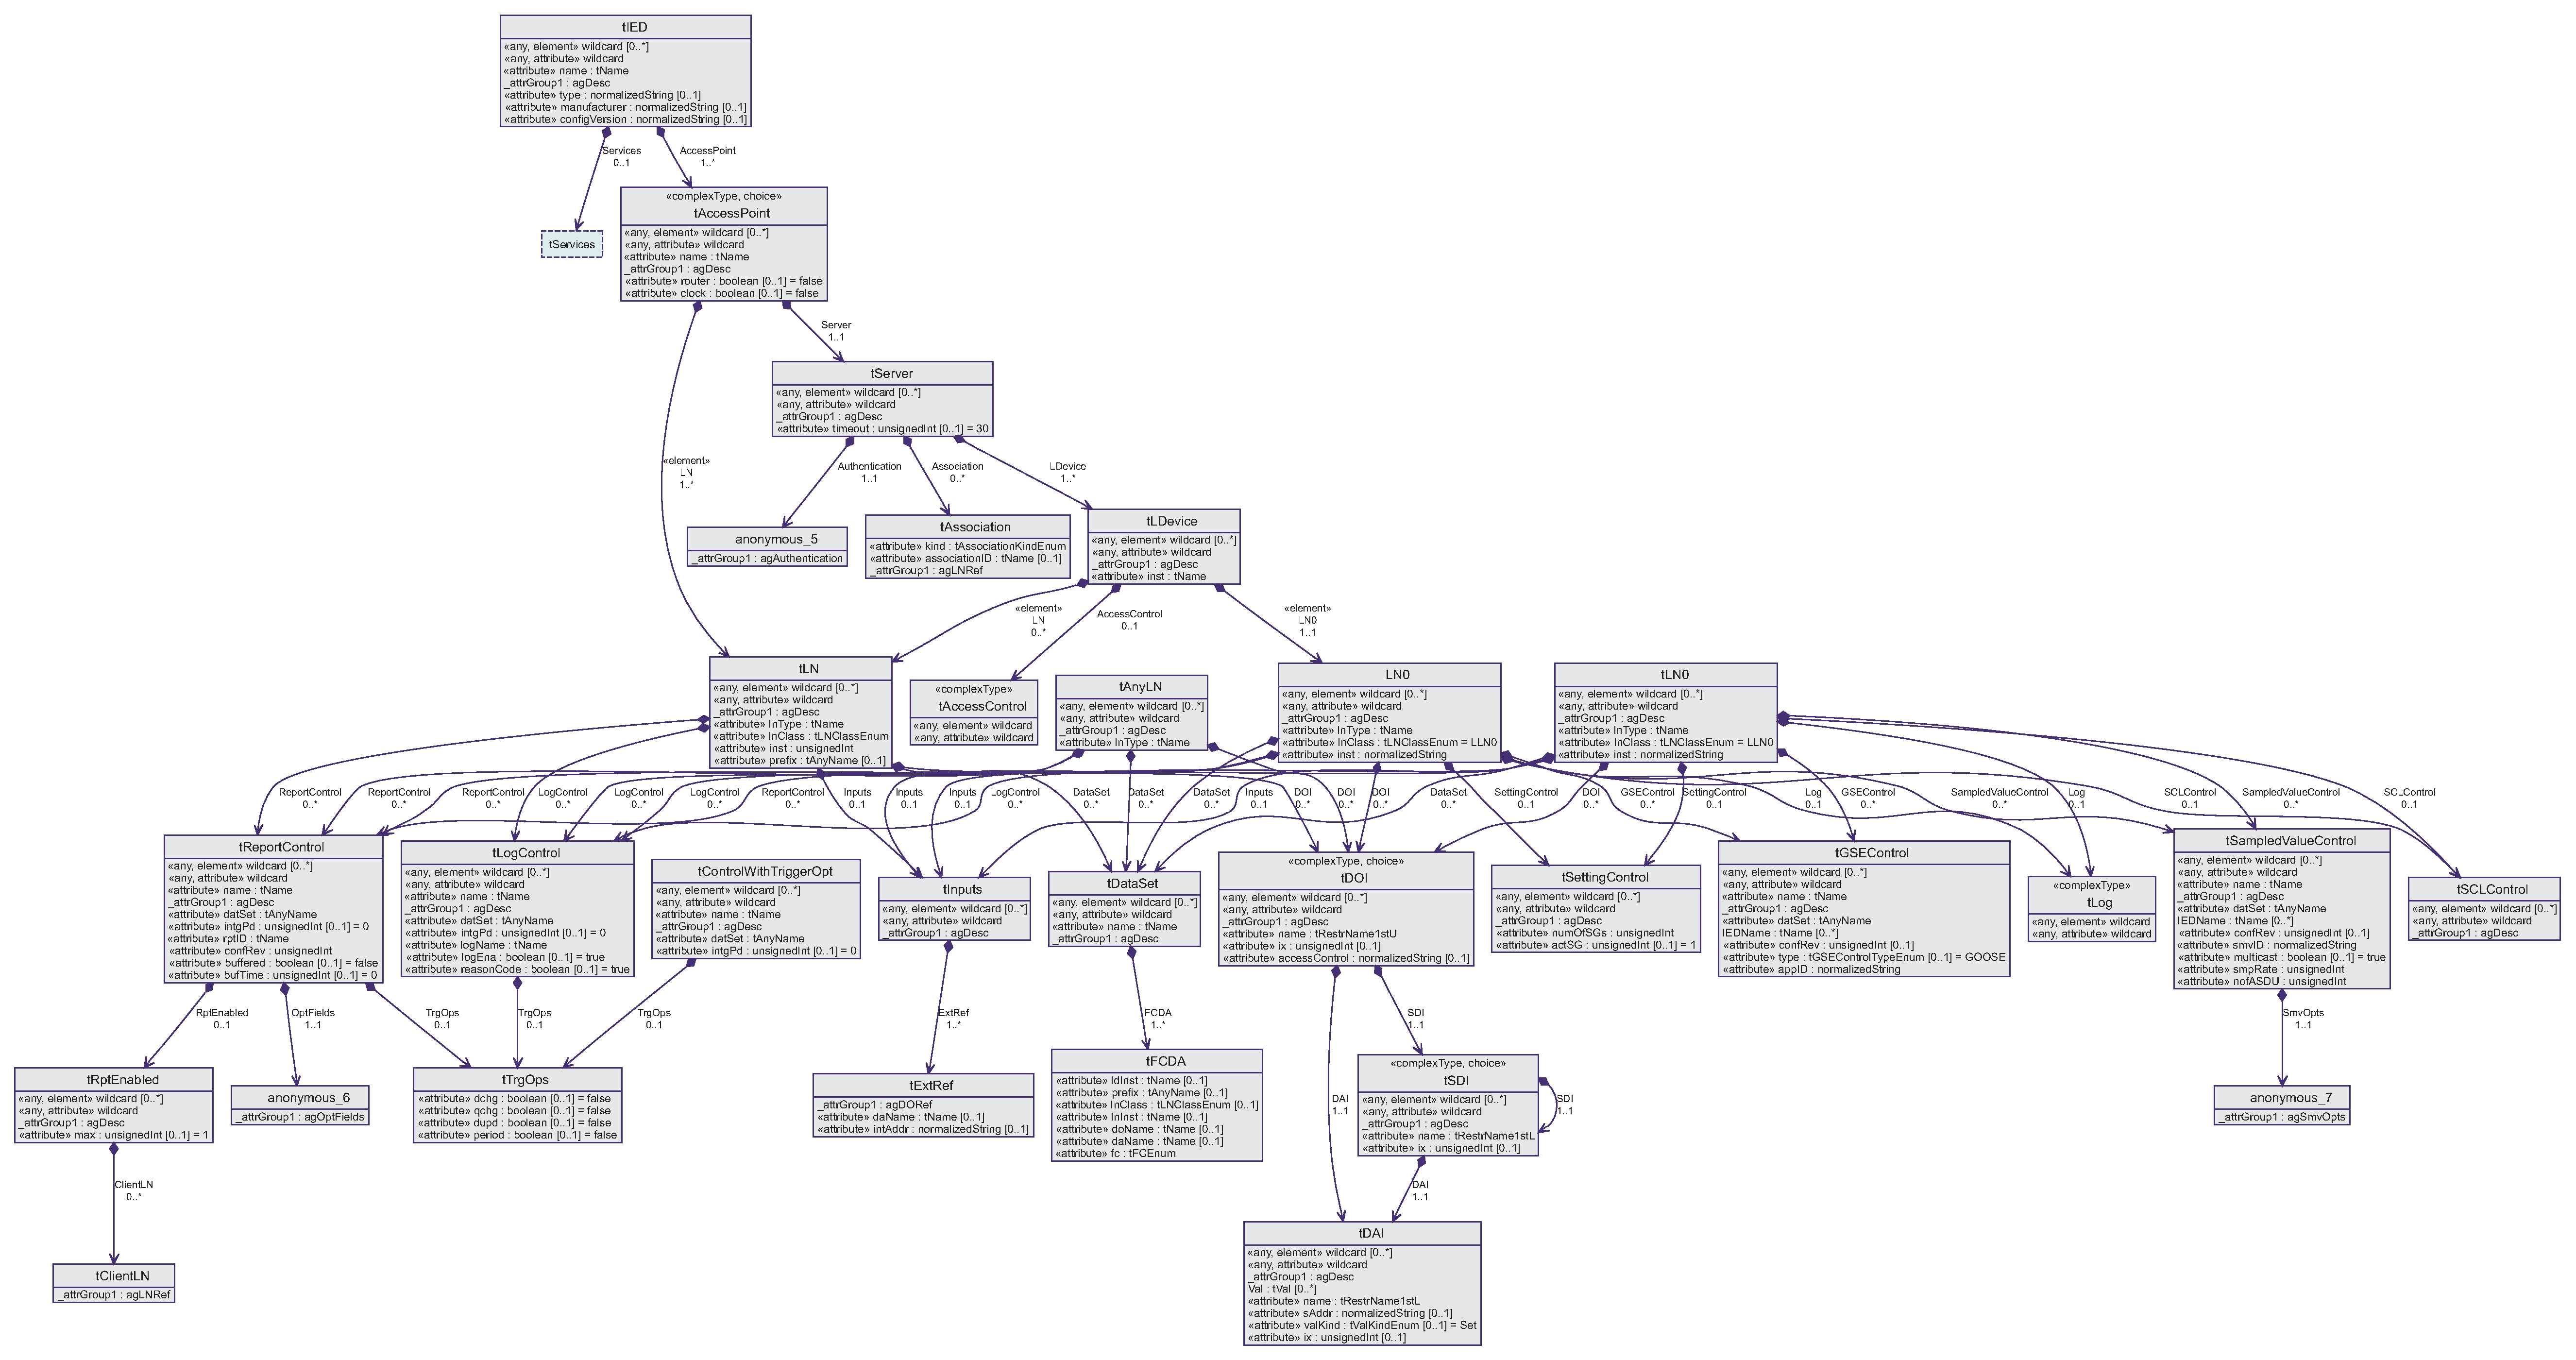
\includegraphics[width=1.0\linewidth]{chapters/enfoque/figures/scl-IED-depthMax-heredado-y-sin-servicios.eps} 
  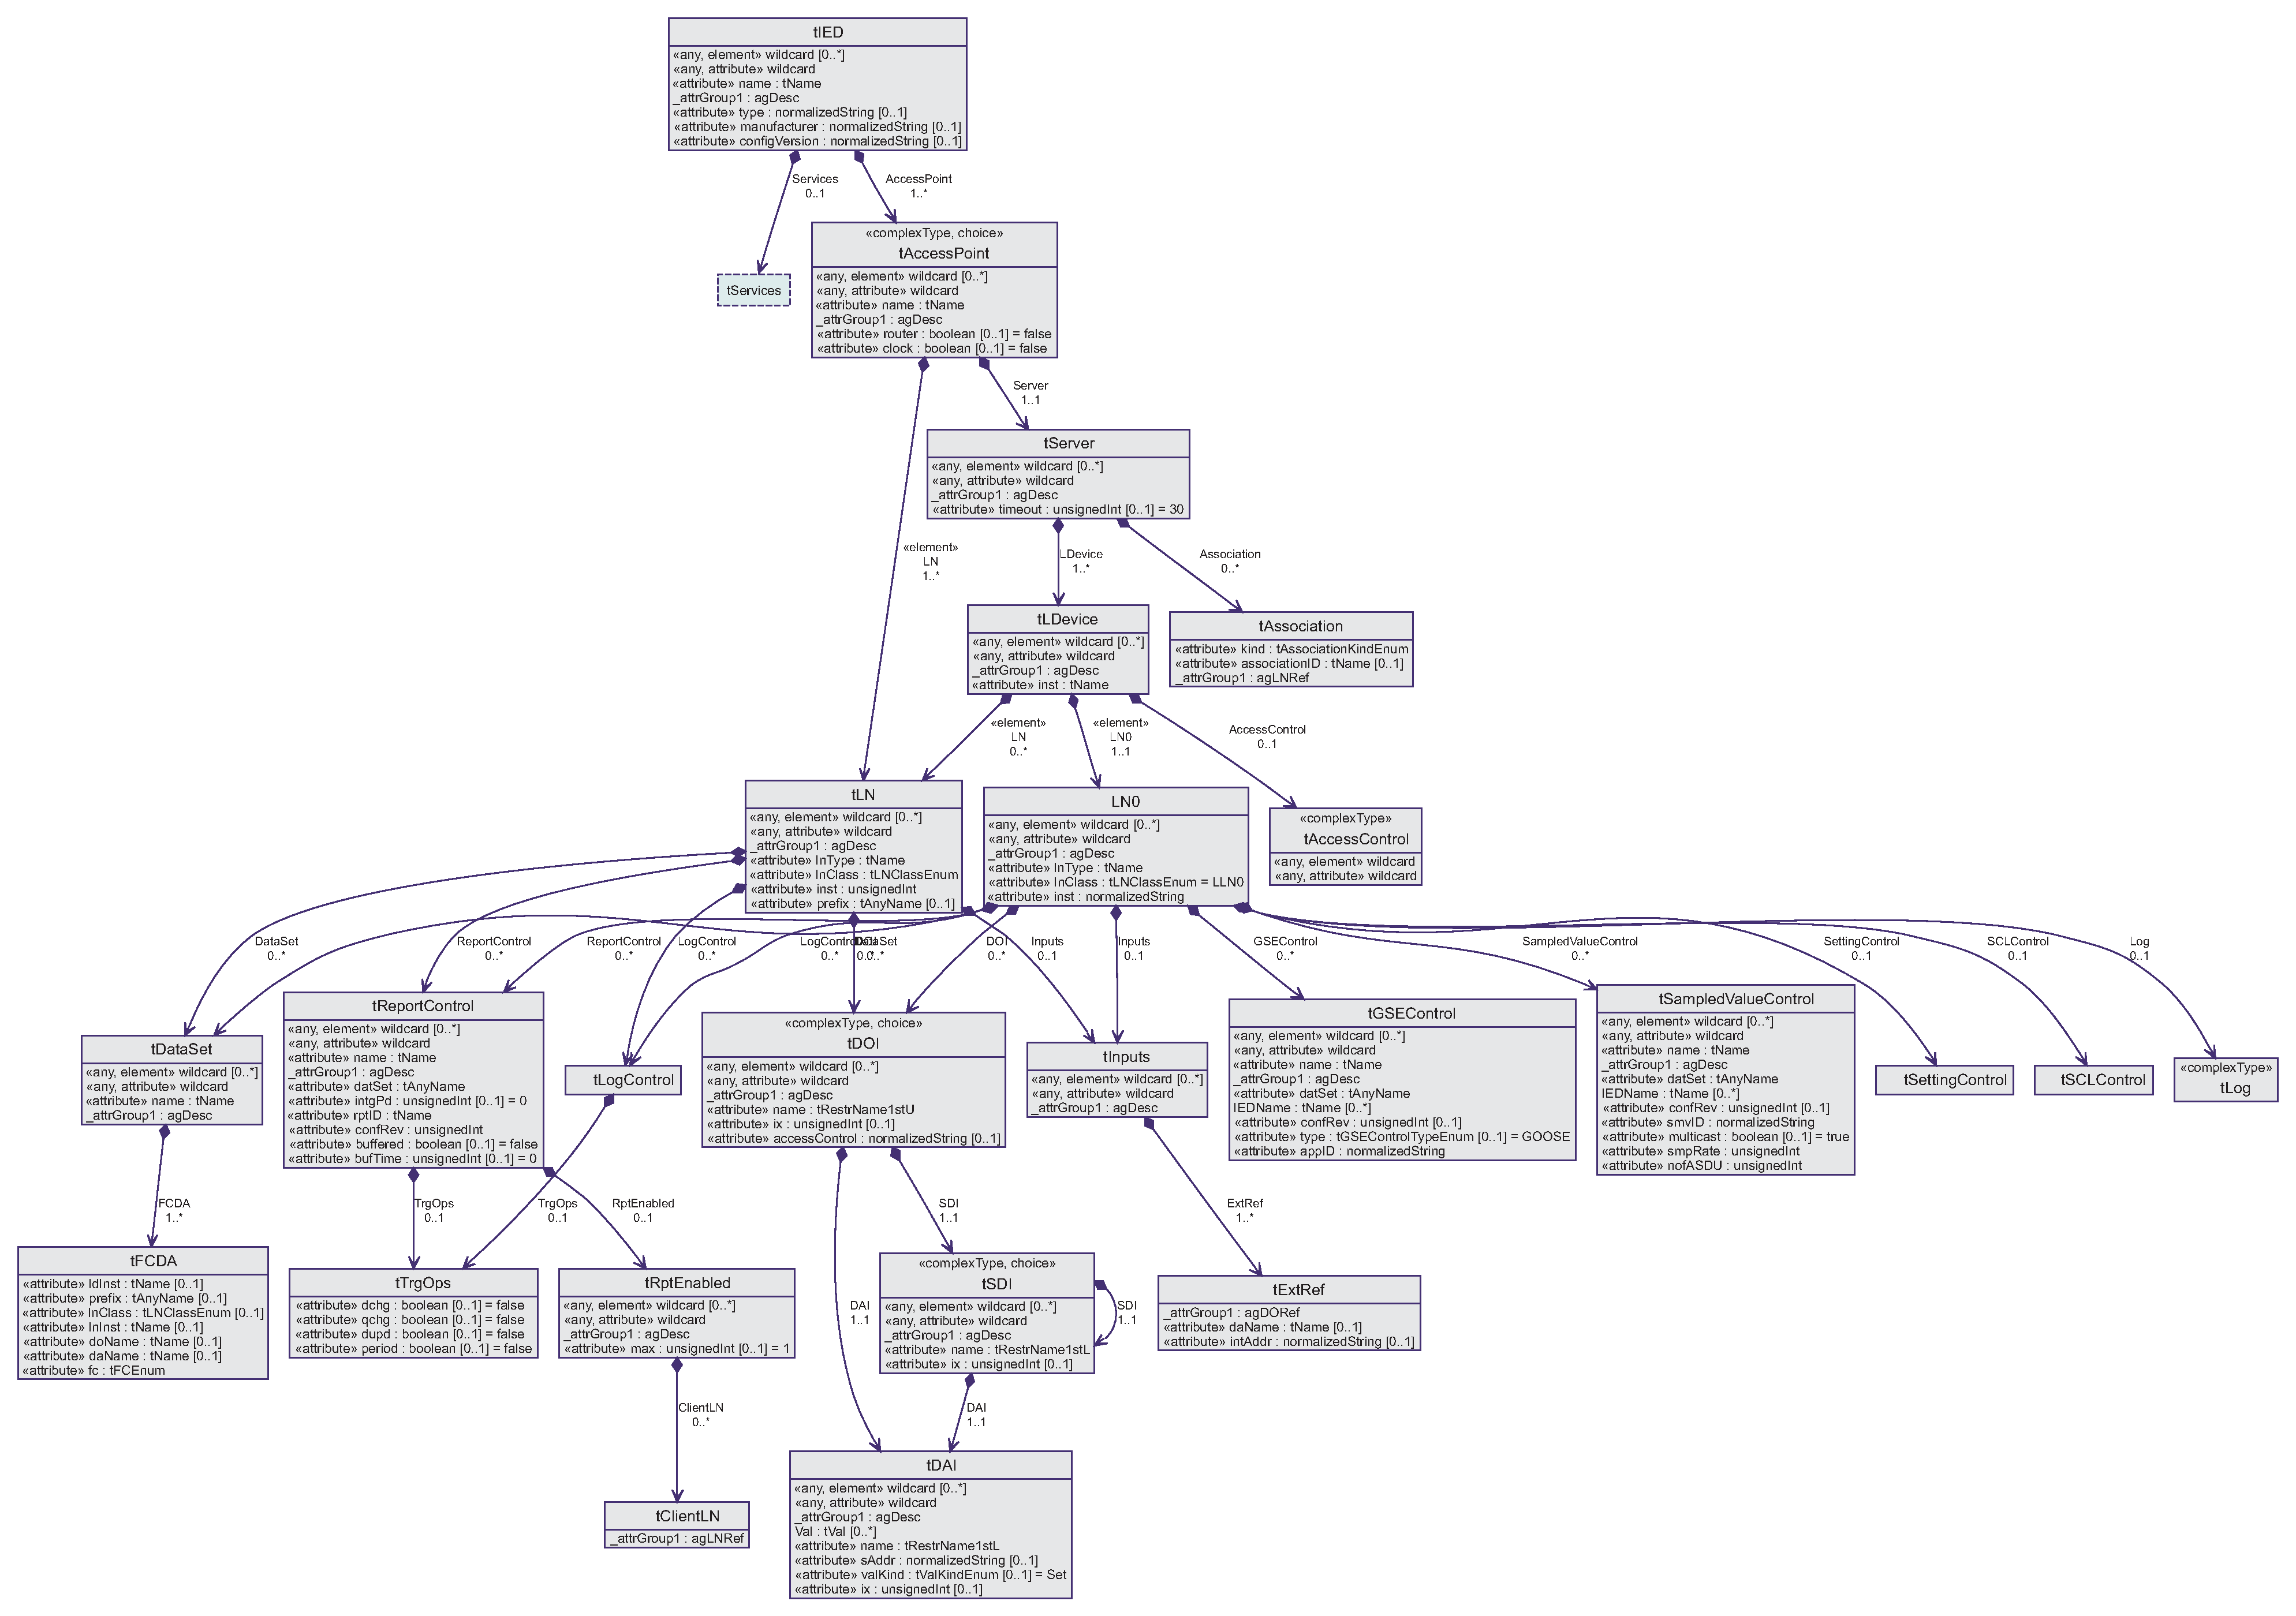
\includegraphics[width=1.0\linewidth]{chapters/enfoque/figures/scl-IED-depthMax-heredado-sin-attributos-y-sin-servicios.eps} 
  \captionsetup{font=scriptsize}
  \caption{Clases del elemento \emph{IED} del SCL, omitiendo sus clases abstractas}
  \label{fig:SCL-IED-depthMax-heredado}
\end{center}
\end{figure}
\end{landscape}

\begin{landscape}
\thispagestyle{empty}
\begin{figure}
\begin{center}
  %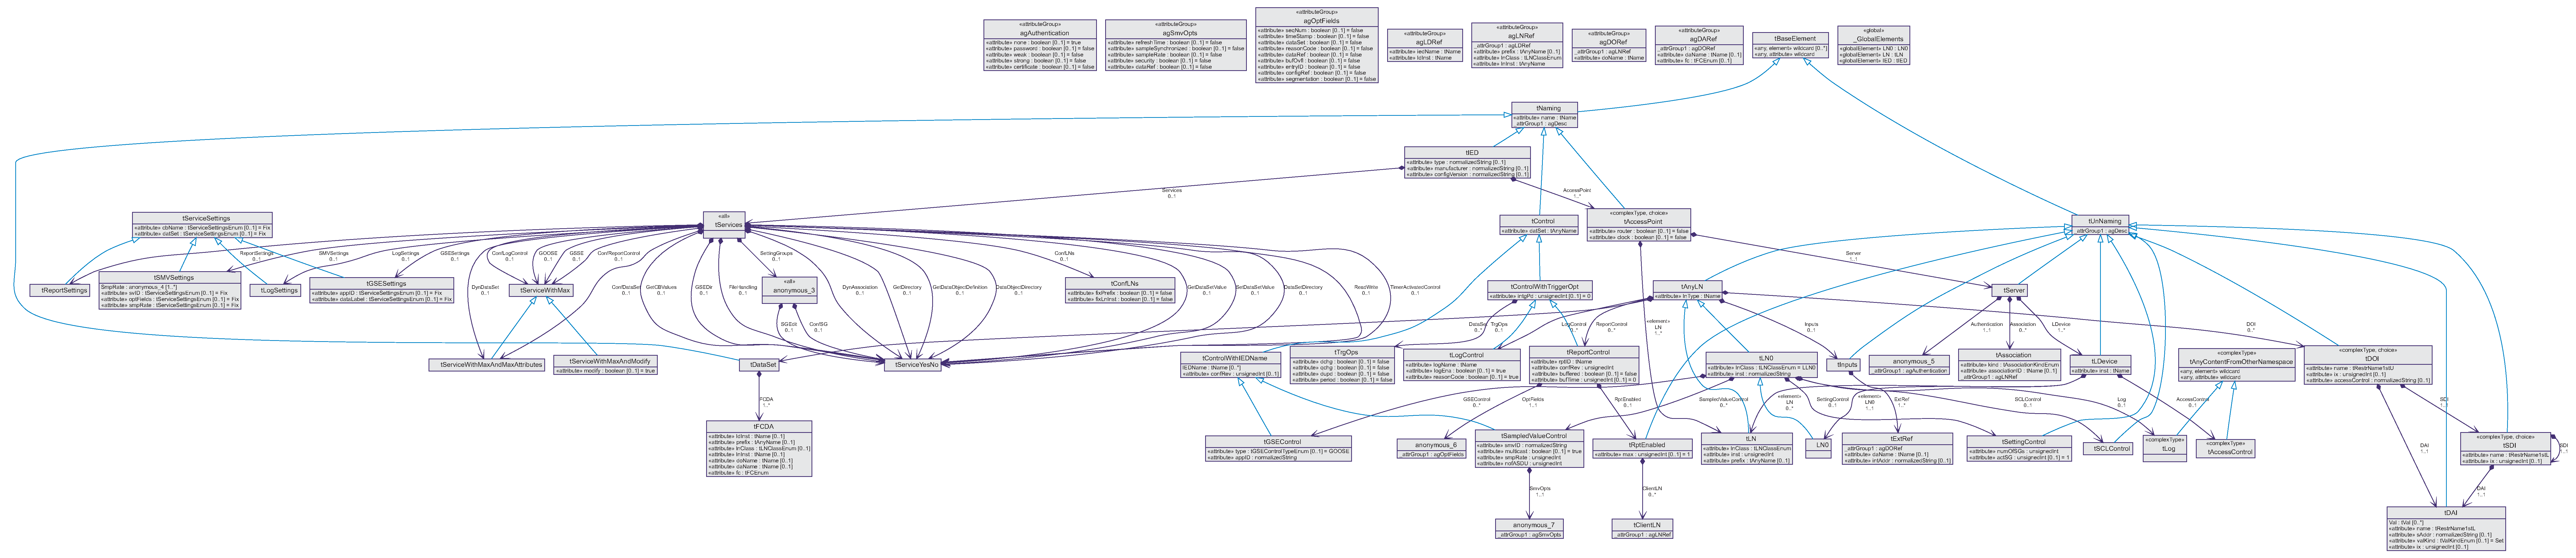
\includegraphics[width=1.0\linewidth]{chapters/enfoque/figures/scl-IED-depthMax-conHerencia.eps} 
  %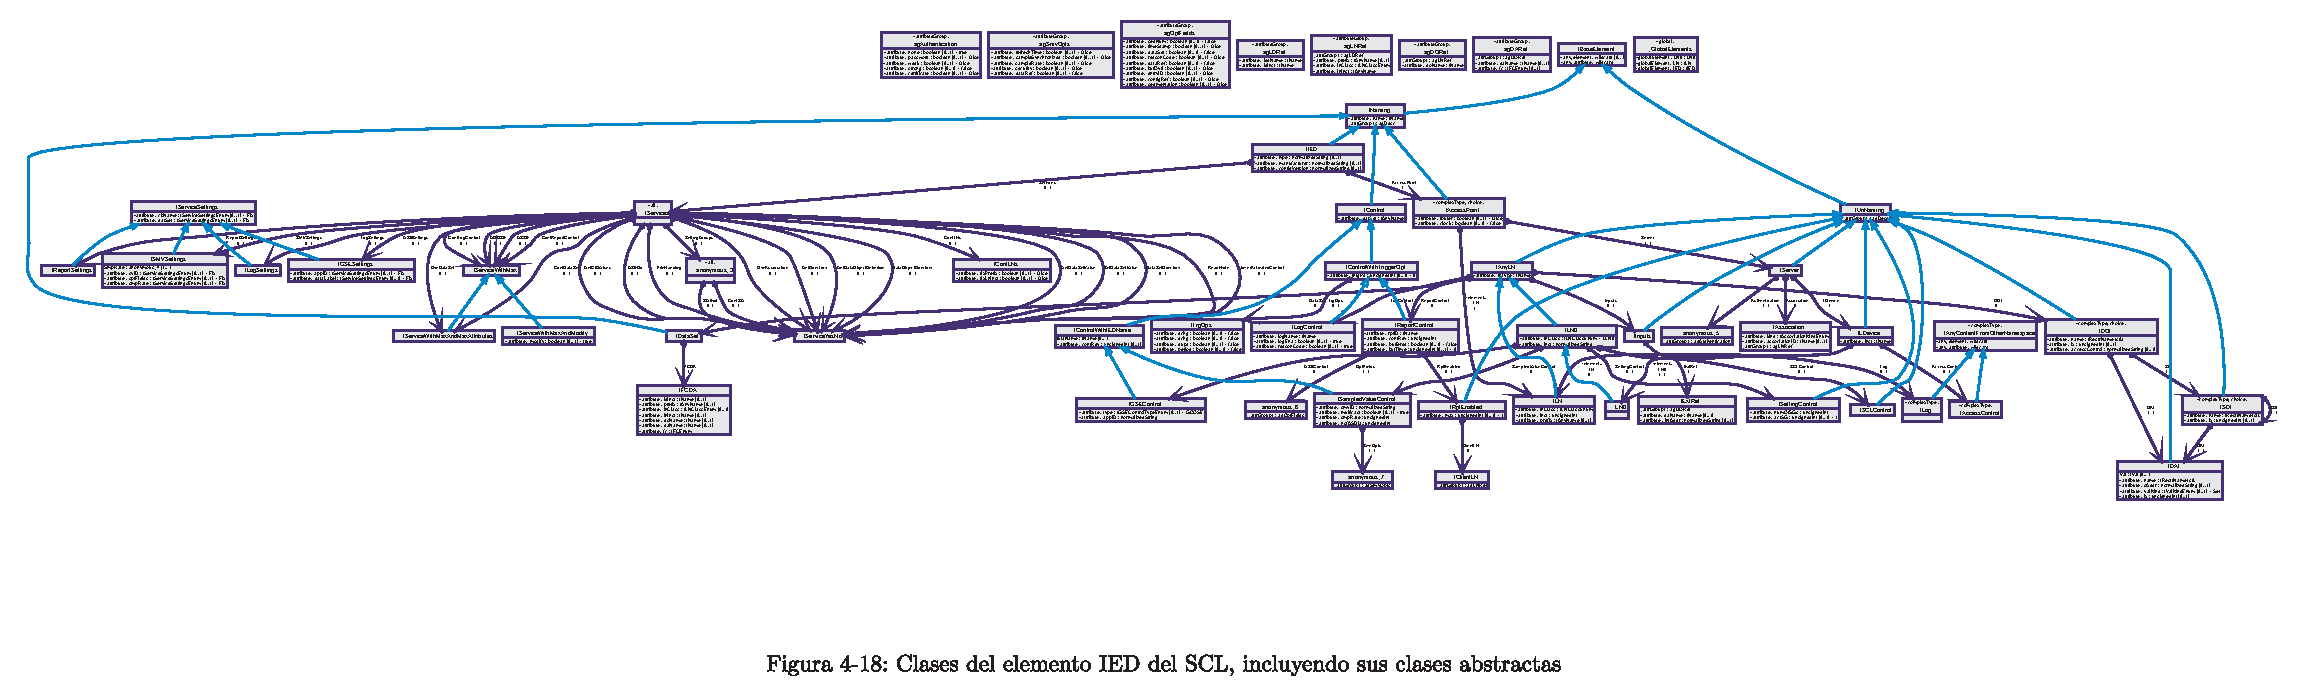
\includegraphics[width=1.0\linewidth]{chapters/enfoque/figures/scl-IED-depthMax-conHerencia-proporcional-a-hoja-A3.eps} 
  %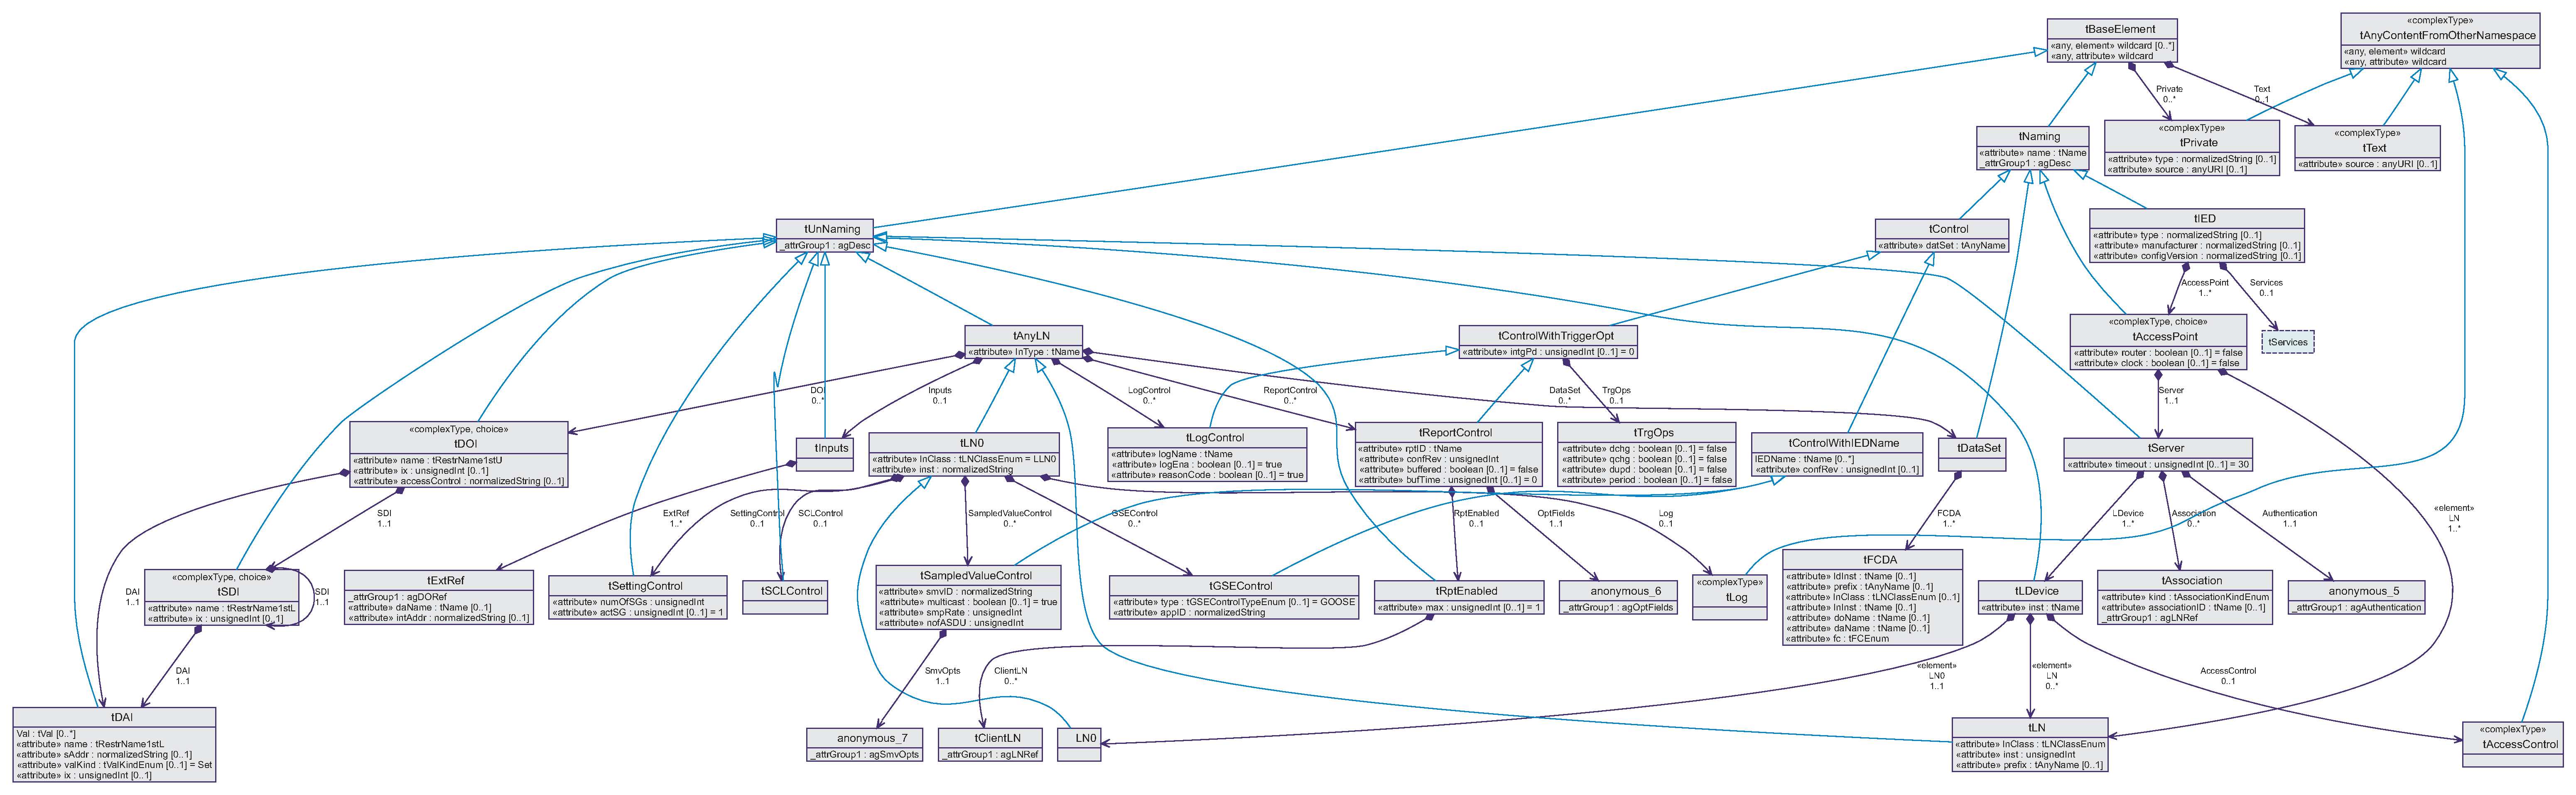
\includegraphics[width=1.0\linewidth]{chapters/enfoque/figures/scl-IED-depthMax-conHerencia-y-sin-Servicios.eps} 
  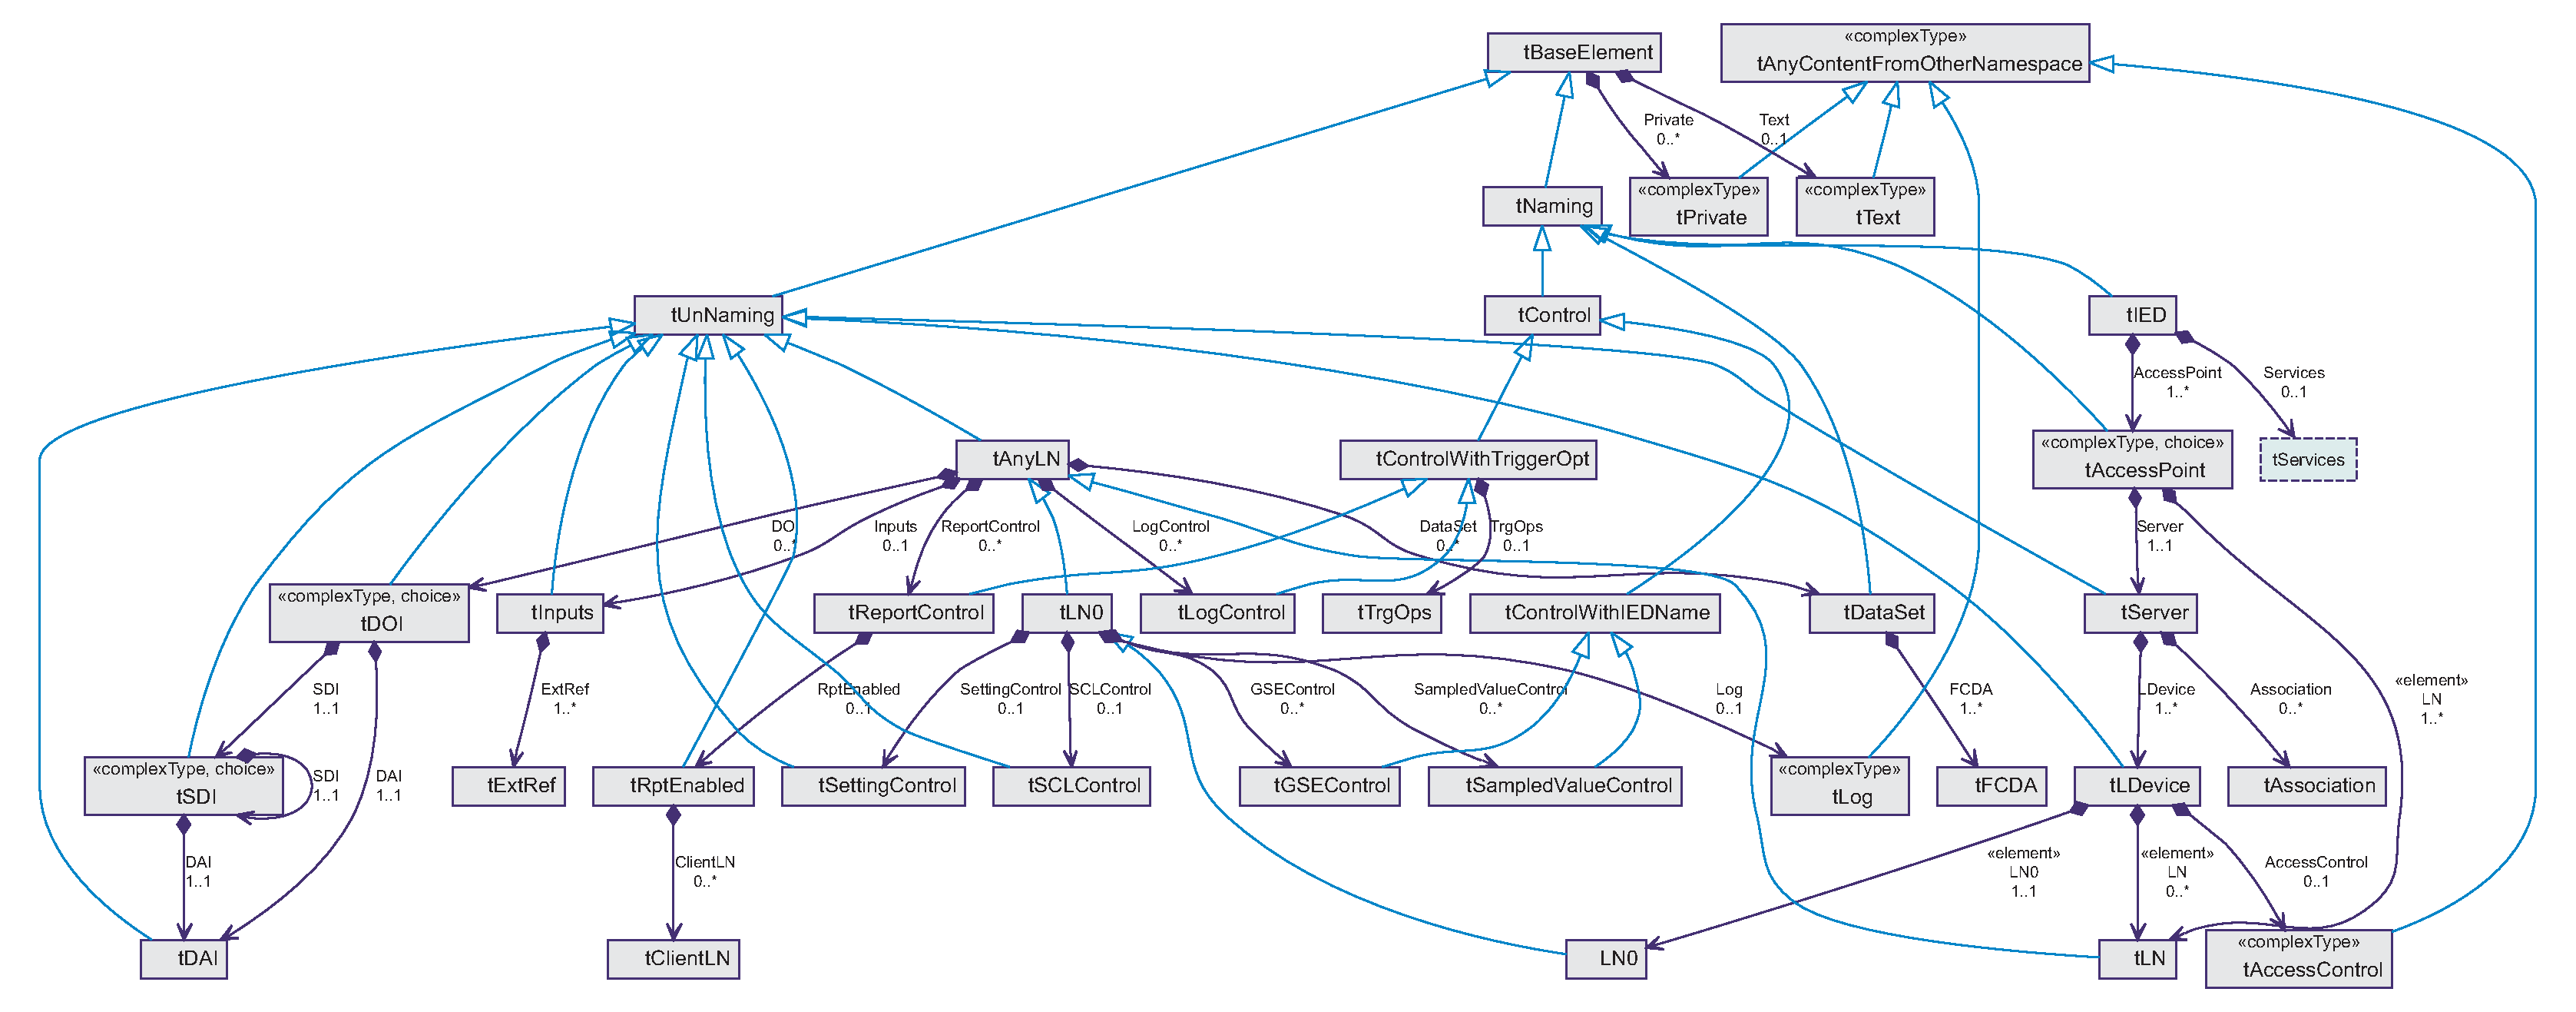
\includegraphics[width=1.0\linewidth]{chapters/enfoque/figures/scl-IED-depthMax-conHerencia-sin-atributos-y-sin-Servicios.eps} 
  \captionsetup{font=scriptsize}
  \caption{Clases del elemento \emph{IED} del SCL, incluyendo sus clases abstractas}
  \label{fig:SCL-IED-depthMax-conHerencia}
\end{center}
\end{figure}
\end{landscape}












%\section{Criterios de dise�o de especificaciones  
de nodos l�gicos que a�n no se ofrecen en el mercado}

\todo[inline]{Tengo que reformular la forma de escribir esta secci�n}

El conocimiento, a grandes rasgos, de los problemas t�cnicos para la
fabricaci�n de dispositivos es muy importante, pues ello permite 
realizar dise�os de sistemas con especificaciones de equipos que, 
si bien no existen en el mercado,
podr�an ser obtenidos con facilidad si los problemas t�cnicos para su
fabricaci�n no son complicados. Por ejemplo, la implementaci�n de
nuevos nodos l�gicos es mas sencilla para el fabricante si este ya ha implementado
anteriormente los CDCs necesarios para el nuevo nodo l�gico. Lo mismo ocurre
con los servicios de comunicaci�n. 
\todo[inline]{aca voy a encajarle las clases java que program� para la 7-x}.
La consideraci�n de este criterio de dise�o es viable gracias a reuniones con
los fabricantes y a la apertura que ofrece la norma al estar basada en
est�ndares abiertos.

\section{Consideraciones para construir sistemas a prueba de futuro}

La norma IEC 61850 abre las posibilidades al proyectista para que este 
pueda construir sistemas a prueba de futuro. Si bien este no es uno 
de los objetivos fundamentales de la norma IEC 61850, 
si el proyectista lo desea, puede considerar ciertos aspectos t�cnicos 
que permitan construir sistemas que perduren en el tiempo.  

El \gls{ACSI} fue dise�ado 
en base al paradigma \gls{O-O-es}, con una estructura muy sencilla (desde el
punto de vista inform�tico) basado en un modelo jer�rquico de la informaci�n.
Su principal objetivo, hablando en t�rminos de dise�o de sofware,  
es desacoplar el dise�o del sistema (el proyecto) de 
la implementaci�n tecnol�gica (los protocolos), 
utilizando el patr�n de dise�o \gls{O-O-es} interface-implementaci�n.

La separaci�n de la interfaz (IEC 61850--7--2) de la implementaci�n 
(IEC 61850--8--x e IEC 61850--9--x) es el compromiso m�s importante que 
la norma IEC 61850 ha tomado para la construcci�n de sistemas a prueba de
futuro. Si bien una buena cantidad de clases del \emph{ACSI} 
son mapeadas directamente al protocolo MMS (osea, el ACSI en realidad no es tan
desacoplado del protocolo MMS), las interfaces existen, funcionan, 
y el proyectista del modelo IEC 61850 no tiene que preocuparse por como se
realiza el mapeado del ACSI a la pila de protocolos de la norma IEC 61850,
igualmente este aspecto es a prueba de futuro. En cuanto
a los protocolos, s�lo hay que
preocuparse por definir sus par�metros adecuadamente.  


El hecho de que a largo plazo se mantengan las interfaces \emph{ACSI} 
facilita una parte importante de la labor del proyectista, pues 
resulta beneficioso apostar por capacitarse en la norma IEC 61850, 
dado que la norma acompa�a de una manera m�s suave los cambios
tecnol�gicos.  

Resulta que el aporte de la norma IEC 61850 no es suficiente 
para construir sistemas a prueba de futuro, a�n resta el 
aporte del proyectista. 
El proyectista debe definir un modelo de datos consistente, 
aprovechando todo el modelo de datos sem�ntico 
proveida por la norma IEC 61850
(utilizando la menor cantidad de nodos l�gicos del grupo G siempre que sea
posible, por ejemplo)
y la posibilidad de describir 
en forma totalmente unificada, organizada y formal 
toda la estructura del sistema IEC 61850 (manteniendo 
un archivo SSD de todo el sistema).
Otros aspectos muy importantes que podr�a definir 
el proyectista para dise�ar sistemas a prueba de futuro
est�n mencionados en la secci�n
\ref{chEnfoque:ied-simplif-no-preconfig}




 





\chapter{Aplicaci�n del enfoque propuesto para el dise�o del modelo IEC 61850
del regulador de velocidad de una unidad generadora t�pica de Itaipu}
\label{cap:model}


\section{Datos del sistema}

%Uno de los primeros pasos del proceso de ingenier�a 
%IEC 61850 consiste en identificar los datos
%disponibles, y en base a estos datos, determinar 
%los nodos l�gicos correspondientes.

En este trabajo se toma como punto de partida los documentos
\emph{Itaipu, aspectos destacados de su ingenier�a} \cite{Itaipu:195860C8841ER0},
\emph{Governing Diagram} \cite{Itaipu:5215DF71167I1R1}, y 
\emph{Governing Diagram -- Description} \cite{Itaipu:52151071168i1r1}, 
donde ya se detallan todos los datos del regulador
de velocidad. Muchos de estos datos no necesariamente
se env�an por la red. Se ha dise�ado el modelo de  
todos los datos posibles para tener un mayor
grado de virtualizaci�n de los sistemas reales, 
de este modo, la programaci�n de las funciones
de control dentro de los IEDs manejan 
datos sem�nticos que podr�an facilitar 
el dise�o de los bloques de control 
dentro del IED o tambi�n el monitoreo del sistema.

Los nodos l�gicos son presentados en un formato tabla. El dise�o del modelo IEC 61850 
presentado en este trabajo se basa en los modelos de nodos l�gicos presentados por esta norma. En 
otras palabras, la combinaci�n seleccionada de nodos l�gicos (modelos de informaci�n definidos por la norma y presentados como
\textbf{DataTypeTemplates} en este trabajo) constituye el dise�o del sistema (modelo de informaci�n del sistema, presentado como
instancias de nodos l�gicos). En resumen, en este cap�tulo se utilizan:
  
\begin{itemize}
	\item Tablas: Enumeran las instancias de un determinado nodo l�gico. Las descripciones incluyen los datos de las unidades generadoras
	de Itaipu.
	\item DataTypeTemplates: Plantillas \textbf{LNType}, del elemento \textbf{DataTypeTemplates}. Estos modelos son extraidos del apartado 7-4-10 
	de la norma IEC 61850 y contiene las descripciones proveidas por esta norma, sin incluir los datos de las unidades generadoras de Itaipu. Cuando 
	el lector desee conocer la aplicaci�n de estas plantillas de nodos l�gicos deber� observar la tabla de instancias del nodo l�gico. 
	\item Descripci�n en \GLS{SCL}: Para ofrecer una descripci�n formal este trabajo tambi�n presenta el dise�o de los modelos 
	de plantillas e instancias usando \GLS{SCL}, que es el lenguaje definido por la norma IEC 61850.
\end{itemize}


\section{Arquitectura del sistema de 
monitoreo y control del regulador de velocidad}

La arquitectura del sistema IEC 61850 definido en este
trabajo tiene las siguientes caracter�sticas:

\begin{itemize}
  \item Topolog�a de red: Anillo.
  \item Redundancia: Sistema totalmente duplicado e id�ntico.
  \item Regulaci�n de velocidad: La regulaci�n primaria y la regulaci�n
  secundaria es realizada en IEDs distintos.
  \item Sensores de frecuencia: Se modelaron ICDs b�sicos
  (conteniendo solamente un nodo l�gico por fase, y suponiendo 
  que la conexi�n del secundario del transformador est�n en 
  estrella para simplificar a�n m�s el modelo) 
  de dos \glspl{MU} para obtener
  la frecuencia del generador y la frecuencia del sistema de potencia.
  \item Sistema Hidr�ulico: El sistema contiene 3 IEDs sensores 
  para la parte hidr�ulica.
  \item Tac�metro: Se ha definido un tac�metro en un ICD. Se 
  han agregado varios nodos l�gicos para el ajuste de curvas, 
  en caso que sea necesario.
\end{itemize} 

La arquitectura general referencial puede visualizarse en la figura
\ref{fig:arquitectura-Gral-Referencial1}. Se ha utilizado 
el layout de la arquitectura general referencial de la 
futura Subestaci�n Villa Hayes \cite{Itaipu:6693DE15207E}.

\begin{landscape}
\thispagestyle{empty}
\begin{figure}
\begin{center}
  \includegraphics[width=0.65\linewidth]{chapters/model/figures/arquitecturaGralReferencial.eps}
  \captionsetup{font=scriptsize}
  \caption{Arquitectura del sistema}
  \label{fig:arquitectura-Gral-Referencial1}
\end{center}
\end{figure}
\end{landscape}
 
\section{Propuesta de extensi�n de los nodos l�gicos de la norma 
IEC 61850-7-410}

El autor de este trabajo propone agregar los siguientes nodos 
l�gicos a la norma IEC 61850:

    
% \subsection{LN: Operation control  -  Name: COPC}
% 
% 	Este nuevo nodo l�gico permite definir el modo de 
% 	operaci�n. Inicialmente, se podr� operar en modo local�simo,
% 	local, desde el sistema central, como as� tambi�n la operaci�n
% 	del equipo podr� realizarse bajo control conjunto. 
% 	
% 
%     \begin{table}[H]
%     \begin{center}
%     \begin{tabular}{|p{3.6cm}|p{2.4cm}|p{6.0cm}|p{0.1cm}|p{0.8cm}|}
%             \hline
%             \multicolumn{5}{|c|}{\cellcolor[gray]{0.8} \textbf{COPC Class} } \\
%             \hline
%             \textbf{Attribute Name} & \textbf{Attr. Type} & \textbf{Explanation} &  \textbf{T} & \textbf{M/O}\\
%             \hline
%             LNName &   & Shall be inherited from Logical-Node Class (see IEC 61850-7-2) & &M \\
%             \hline
%             \multicolumn{5}{|l|}{\cellcolor[gray]{0.8} \textbf{Data} } \\
%             \hline
% 
% 			\multicolumn{5}{|l|}{\textbf{Common Logical Node Information} } \\
%             \hline
%               &  &LN shall inherit all Mandatory Data from Common Logical Node Class & & \\
%             \hline
% 
% 			\multicolumn{5}{|l|}{\textbf{Controls} } \\
%             \hline
%             OpLcls  & ACT  & Operaci�n en modo local�simo & & O\\
%             \hline
%             OpLcl  & ACT  & Operaci�n en modo local & & O\\
%             \hline
%             OpCntr  & ACT & Operaci�n desde el control central & & O\\
%             \hline
%             OpCnj  & ACT & Operaci�n bajo control conjunto & & O\\
%             \hline
% 			\end{tabular}
%     \caption{Nuevo nodo l�gico: COPC}
%     \label{table:newLN-COPC}
%     \end{center}
%     \end{table}
% 
% 
% \todo{traducir los DATA al ingles!}
% 
%     

\subsection{LN: Hydraulic switch  -  Name: SSWI}

	Este nuevo nodo l�gico podr�a ser utilizado para modelar 
	swiches
	de los sistemas mec�nicos. Este nodo l�gico permite conocer 
	la posici�n de la llave hidr�ulica. Resulta que el 
	nodo l�gico TPOS env�a mensajes con los protocolos definidos 
	en IEC 61850-9-x del porcentaje de abertura o cierre, por lo tanto, no siempre
	se obtendr� un buen desempe�o del flujo de informaci�n circulante por la red si
	la llave selectora digital es escalonada (si tiene solamente dos o tres
	posiciones fijas por ejemplo). En estos casos resulta exagerado el uso 
	del bus de proceso con el \textbf{CDC SAV}, por lo que el autor de este trabajo
	propone agregar este nodo l�gico a la norma IEC 61850.
    El item 22 del regulador Rapid77 \cite{Itaipu:52151071168i1r1}, llaves de
    velocidad, tambi�n podr�a ser modelado con este nodo l�gico.
	
	Este nodo l�gico es muy similar al \textbf{HITG}, pero tiene 
	la sem�ntica adecuada.
	

    \begin{table}[H]
    \begin{center}
    \begin{tabular}{|p{3.6cm}|p{2.4cm}|p{6.0cm}|p{0.1cm}|p{0.8cm}|}
            \hline
            \multicolumn{5}{|c|}{\cellcolor[gray]{0.8} \textbf{SSWI Class} } \\
            \hline
            \textbf{Attribute Name} & \textbf{Attr. Type} & \textbf{Explanation} &  \textbf{T} & \textbf{M/O}\\
            \hline
            LNName &   & Shall be inherited from Logical-Node Class (see IEC 61850-7-2) & &M \\
            \hline
            \multicolumn{5}{|l|}{\cellcolor[gray]{0.8} \textbf{Data} } \\
            \hline

			\multicolumn{5}{|l|}{\textbf{Common Logical Node Information} } \\
            \hline
              &  &LN shall inherit all Mandatory Data from Common Logical Node Class & & \\
            \hline

			\multicolumn{5}{|l|}{\textbf{Status information} } \\
			\hline
			SwTyp & INS & Switch type & & M\\
			\hline
			SwOpCap & INS & Switch operating capability && M\\
            \hline
            PosStep  & INS & Integer representing the position, counting from
            lowest position & & O\\
            \hline
            PosUp  & SPS & Upper end position reached (switch cannot move
            further)& & M\\
            \hline
            PosDn  & PosDn & Lower end position reached (switch cannot move
            further) & & M\\
            \hline
            Mvm  & SPS & Switch is moving & & O\\
            \hline
			SwBlk & SPS & Switch is blocked (cannot move from present position) & &O\\
            \hline

			\multicolumn{5}{|l|}{\textbf{Controls} } \\
             \hline
             Opn  & SPC  & Switch to full open position & & O\\
             \hline
             Cls  & SPC &  Switch to full closed position & & O\\
             \hline
             BlkOpn  & SPC & Block opening of the switch & & O\\
             \hline
             BlkCls  & SPC & Block closing of the gate & & O\\
             \hline
			\end{tabular}
    \caption{Nuevo nodo l�gico: SSWI}
    \label{table:newLN-COPC}
    \end{center}
    \end{table}

En donde SwOpCap es una enumeraci�n que representa las 
capacidades f�sicas de operaci�n de la llave o v�lvula.
\begin{itemize}
  \item None: 1
  \item Open: 2
  \item Close: 3
  \item Open and Close: 4
\end{itemize}

Este nodo l�gico est� dise�ado para trabajar en conjunto 
con el nodo l�gico \textbf{CSWI} en caso que sea necesario. 
El nodo l�gico \textbf{XSWI} no reemplaza a este nuevo nodo l�gico 
pues el \textbf{XSWI} fue concebido para llaves de apertura 
de circuitos el�ctricos, no hidr�ulicos ni neum�ticos.

\subsection{LN: Frecuency sensor  -  Name: SFRQ}

El nodo l�gico \textbf{SFRQ} representar�a un sensor de frecuencia el�ctrica
que permita enviar los valores muestreados de frecuencia por la IEC 61850-9-x (a trav�s del \GLS{CDC} \textbf{SAV}).
El nodo l�gico \textbf{MMXU} s�lo realiza mediciones, no se permite utilizarlo para valores muestreados, 
los nodos l�gicos \textbf{TFRQ} y \textbf{TRTN} son espec�ficos para el env�o
de la frecuencia no el�ctrica. El regulador de velocidad de Itaipu
necesita las frecuencias el�ctricas medidas
en la barra de 13KV y en la barra de 500KV. En el dise�o se 
ha utilizado el nodo l�gico \textbf{TVTR}.

	
	

    \begin{table}[H]
    \begin{center}
    \begin{tabular}{|p{3.6cm}|p{2.4cm}|p{6.0cm}|p{0.1cm}|p{0.8cm}|}
            \hline
            \multicolumn{5}{|c|}{\cellcolor[gray]{0.8} \textbf{SFRQ Class} } \\
            \hline
            \textbf{Attribute Name} & \textbf{Attr. Type} & \textbf{Explanation} &  \textbf{T} & \textbf{M/O}\\
            \hline
            LNName &   & Shall be inherited from Logical-Node Class (see IEC 61850-7-2) & &M \\
            \hline
            \multicolumn{5}{|l|}{\cellcolor[gray]{0.8} \textbf{Data} } \\
            \hline

 
			\multicolumn{5}{|l|}{\textbf{Common Logical Node Information} } \\
            \hline
              &  &LN shall inherit all Mandatory Data from Common Logical Node Class & & \\
            \hline
            EEHealth & INS & External equipment health & & O\\
            \hline
            EEName & DPL & External equipment name plate & & O\\
            \hline
            OpTmh & INS & Operation time & & O\\
            \hline


			\multicolumn{5}{|l|}{\textbf{Measured values} } \\
            \hline
            Hz  & SAV & Frecuency (sampled value)& & M\\
            \hline


			\multicolumn{5}{|l|}{\textbf{Status Information} } \\
            \hline
            FuFail & SPS & TVTR fuse failure& & O\\
            \hline
			\multicolumn{5}{|l|}{\textbf{Settings} } \\
            \hline
            HzRtg  & ASG & Rated frecuency & & O\\
            \hline
			\end{tabular}
    \caption{Nuevo nodo l�gico: SFRQ}
    \label{table:newLN-SFRQ}
    \end{center}
    \end{table}



    
    
\section{Nodos l\'ogicos del IED IEDRV}
\label{sec:LNs-del-IEDRV}

En la figura \ref{fig:MODEL-resumen-IEDRV} se presenta un resumen
de los nodos l�gicos m�s importantes, y en las tablas a continuaci�n se 
presentan los detalles correspondientes.

Los nodos l�gicos de esta secci�n corresponden
a los IEDs reguladores de velocidad (primaria y secundaria). Los 
IEDs son id�nticos. Simplemente cambian los algoritmos internos 
basados en los nodos l�gicos \textbf{FPID}.

\begin{figure}
\begin{center}
  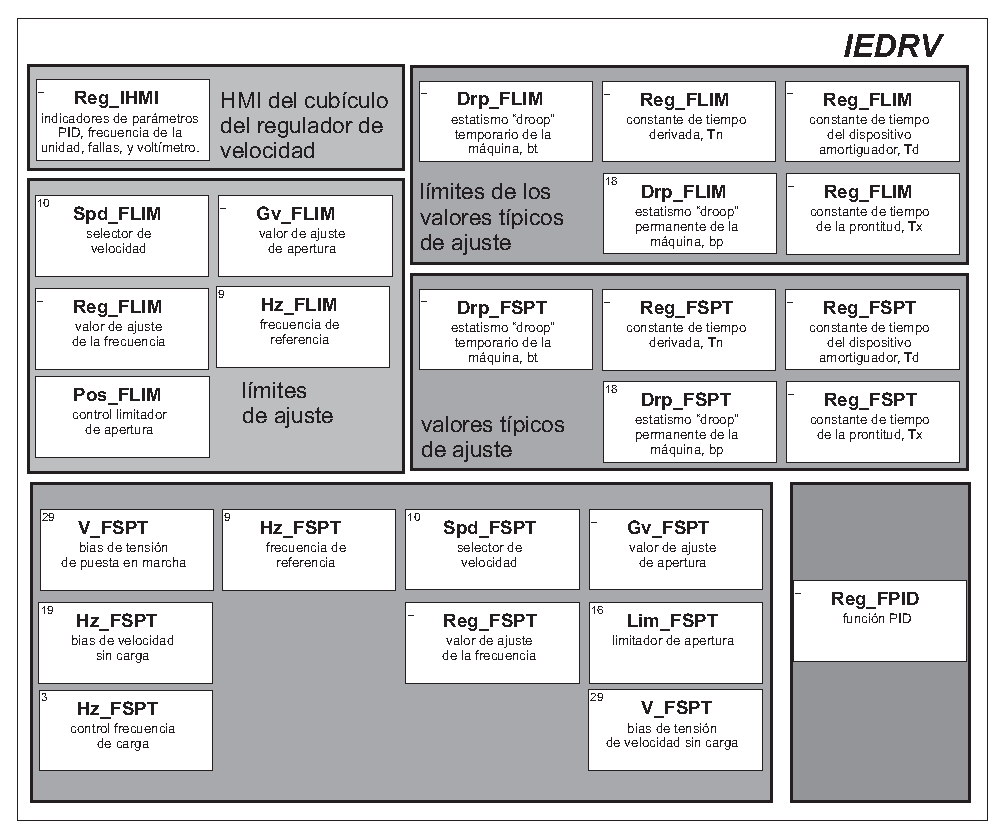
\includegraphics[width=0.7\linewidth]{chapters/model/figures/LN-IEDRV.eps} 
  \caption{Resumen de los nodos l�gicos m�s importantes del IED \emph{IEDRV}}
  \label{fig:MODEL-resumen-IEDRV}
\end{center}
\end{figure}

\input{chapters/model/iedE/FPID_reg} 


\input{chapters/model/iedE/FLIM_tipical} 
  
  
\input{chapters/model/iedE/FSPT_1} 
  
  
  
  

    
\section{Nodos l\'ogicos del IED IEDMainTnk}
\input{chapters/model/iedA/FLIM_} 
  
  
\input{chapters/model/iedA/FXOT_1} 
  
  
\input{chapters/model/iedA/FXUT_1} 
  
  
\input{chapters/model/iedA/KFIL_29} 
  
  
\input{chapters/model/iedA/KFIL_actuator} 
  
  
\input{chapters/model/iedA/KPMPa} 
  
  
\input{chapters/model/iedA/KTNK_1} 
  
  
\input{chapters/model/iedA/KVLV_idler_system} 
  
  
\input{chapters/model/iedA/KVLV_adjusting_isolating_valve} 
  
  
\input{chapters/model/iedA/KVLV_piloted} 
  
  
\input{chapters/model/iedA/KVLV_solenoid_operated} 
  
  
\input{chapters/model/iedA/KVLV_restrictor} 
  
  
\input{chapters/model/iedA/KVLV_switch} 
  
  
\input{chapters/model/iedA/STMP6} 
  
  
\input{chapters/model/iedA/STMP_thermostat} 
  
  
\input{chapters/model/iedA/TLEV_gauge} 
  
  
\input{chapters/model/iedA/TPOS_e} 
  
  
\input{chapters/model/iedA/TPOS_lvl_sw} 
  
  
\input{chapters/model/iedA/TPOS_prs_sw} 
  
  
\input{chapters/model/iedA/TPRS_gauge} 
  
  
\input{chapters/model/iedA/TTMP_6} 
  
  
\input{chapters/model/iedA/TTMP_thermostat} 
  
  
\input{chapters/model/iedA/ZMOTa} 
  
  

    
\section{Nodos l\'ogicos del IED IEDairOilTNK}
\input{chapters/model/iedB/KTNK_air_oil} 
  
  
\input{chapters/model/iedB/KVLV_solenoid_operated} 
  
  
\input{chapters/model/iedB/KVLV_relief} 
  
  
\input{chapters/model/iedB/KVLV_aut_contr} 
  
  
\input{chapters/model/iedB/TLEV_gauge} 
  
  
\input{chapters/model/iedB/TPOS_prs_sw} 
  
  
\input{chapters/model/iedB/TPRS_trans} 
  
  
\input{chapters/model/iedB/TPRS_gauge} 
  
  

    
\section{Nodos l\'ogicos del IED IEDcmprsAirPlant}
\input{chapters/model/iedC/FLIM_} 
  
  
\input{chapters/model/iedC/FSPT_for_flim} 
  
  
\input{chapters/model/iedC/KVLV_relief} 
  
  
\input{chapters/model/iedC/TPOS_e} 
  
  
\input{chapters/model/iedC/TPOS_prs_sw} 
  
  
\input{chapters/model/iedC/TPRS_gauge} 
  
  
\input{chapters/model/iedC/ZMOTa} 
  
  

    
\section{Nodos l\'ogicos del IED IEDsensRot}
\input{chapters/model/iedD/FLIM_tipical} 
  
  
\input{chapters/model/iedD/FSPT_1} 
  
  
\input{chapters/model/iedD/TRTN_1} 
  
  
\input{chapters/model/iedD/HSPD_1} 
  
  


\section{Resumen de los nodos l�gicos del sistema}

En la figura \ref{fig:LNodes-reg-veloc} se presenta el resumen gr�fico de los 
nodos l�gicos del regulador de velocidad, conforme a la arquitectura definida en la figura \ref{fig:arquitectura-Gral-Referencial1}.
Este gr�fico fue generado por la herramienta de ingenier�a Atlan61850 a partir de los archivos ICD del anexo \ref{app:resultados2-codigos-SCL}, 
y los XSDs del anexo A de la norma IEC 61850--6 \cite{IEC61850-6:2004}, 
que han sido modificados para utilizar las definiciones de norma IEC 61850--7--4--10 \cite{IEC61850-7-410:2007} (estas modificaciones 
se presentan en el anexo \ref{app:codigos-SCL} de este trabajo).
Posteriormente el gr�fico fue enriquecido utilizando 
un editor de im�genes convencional.

\begin{landscape}
\thispagestyle{empty}
\begin{figure}
\begin{center}
  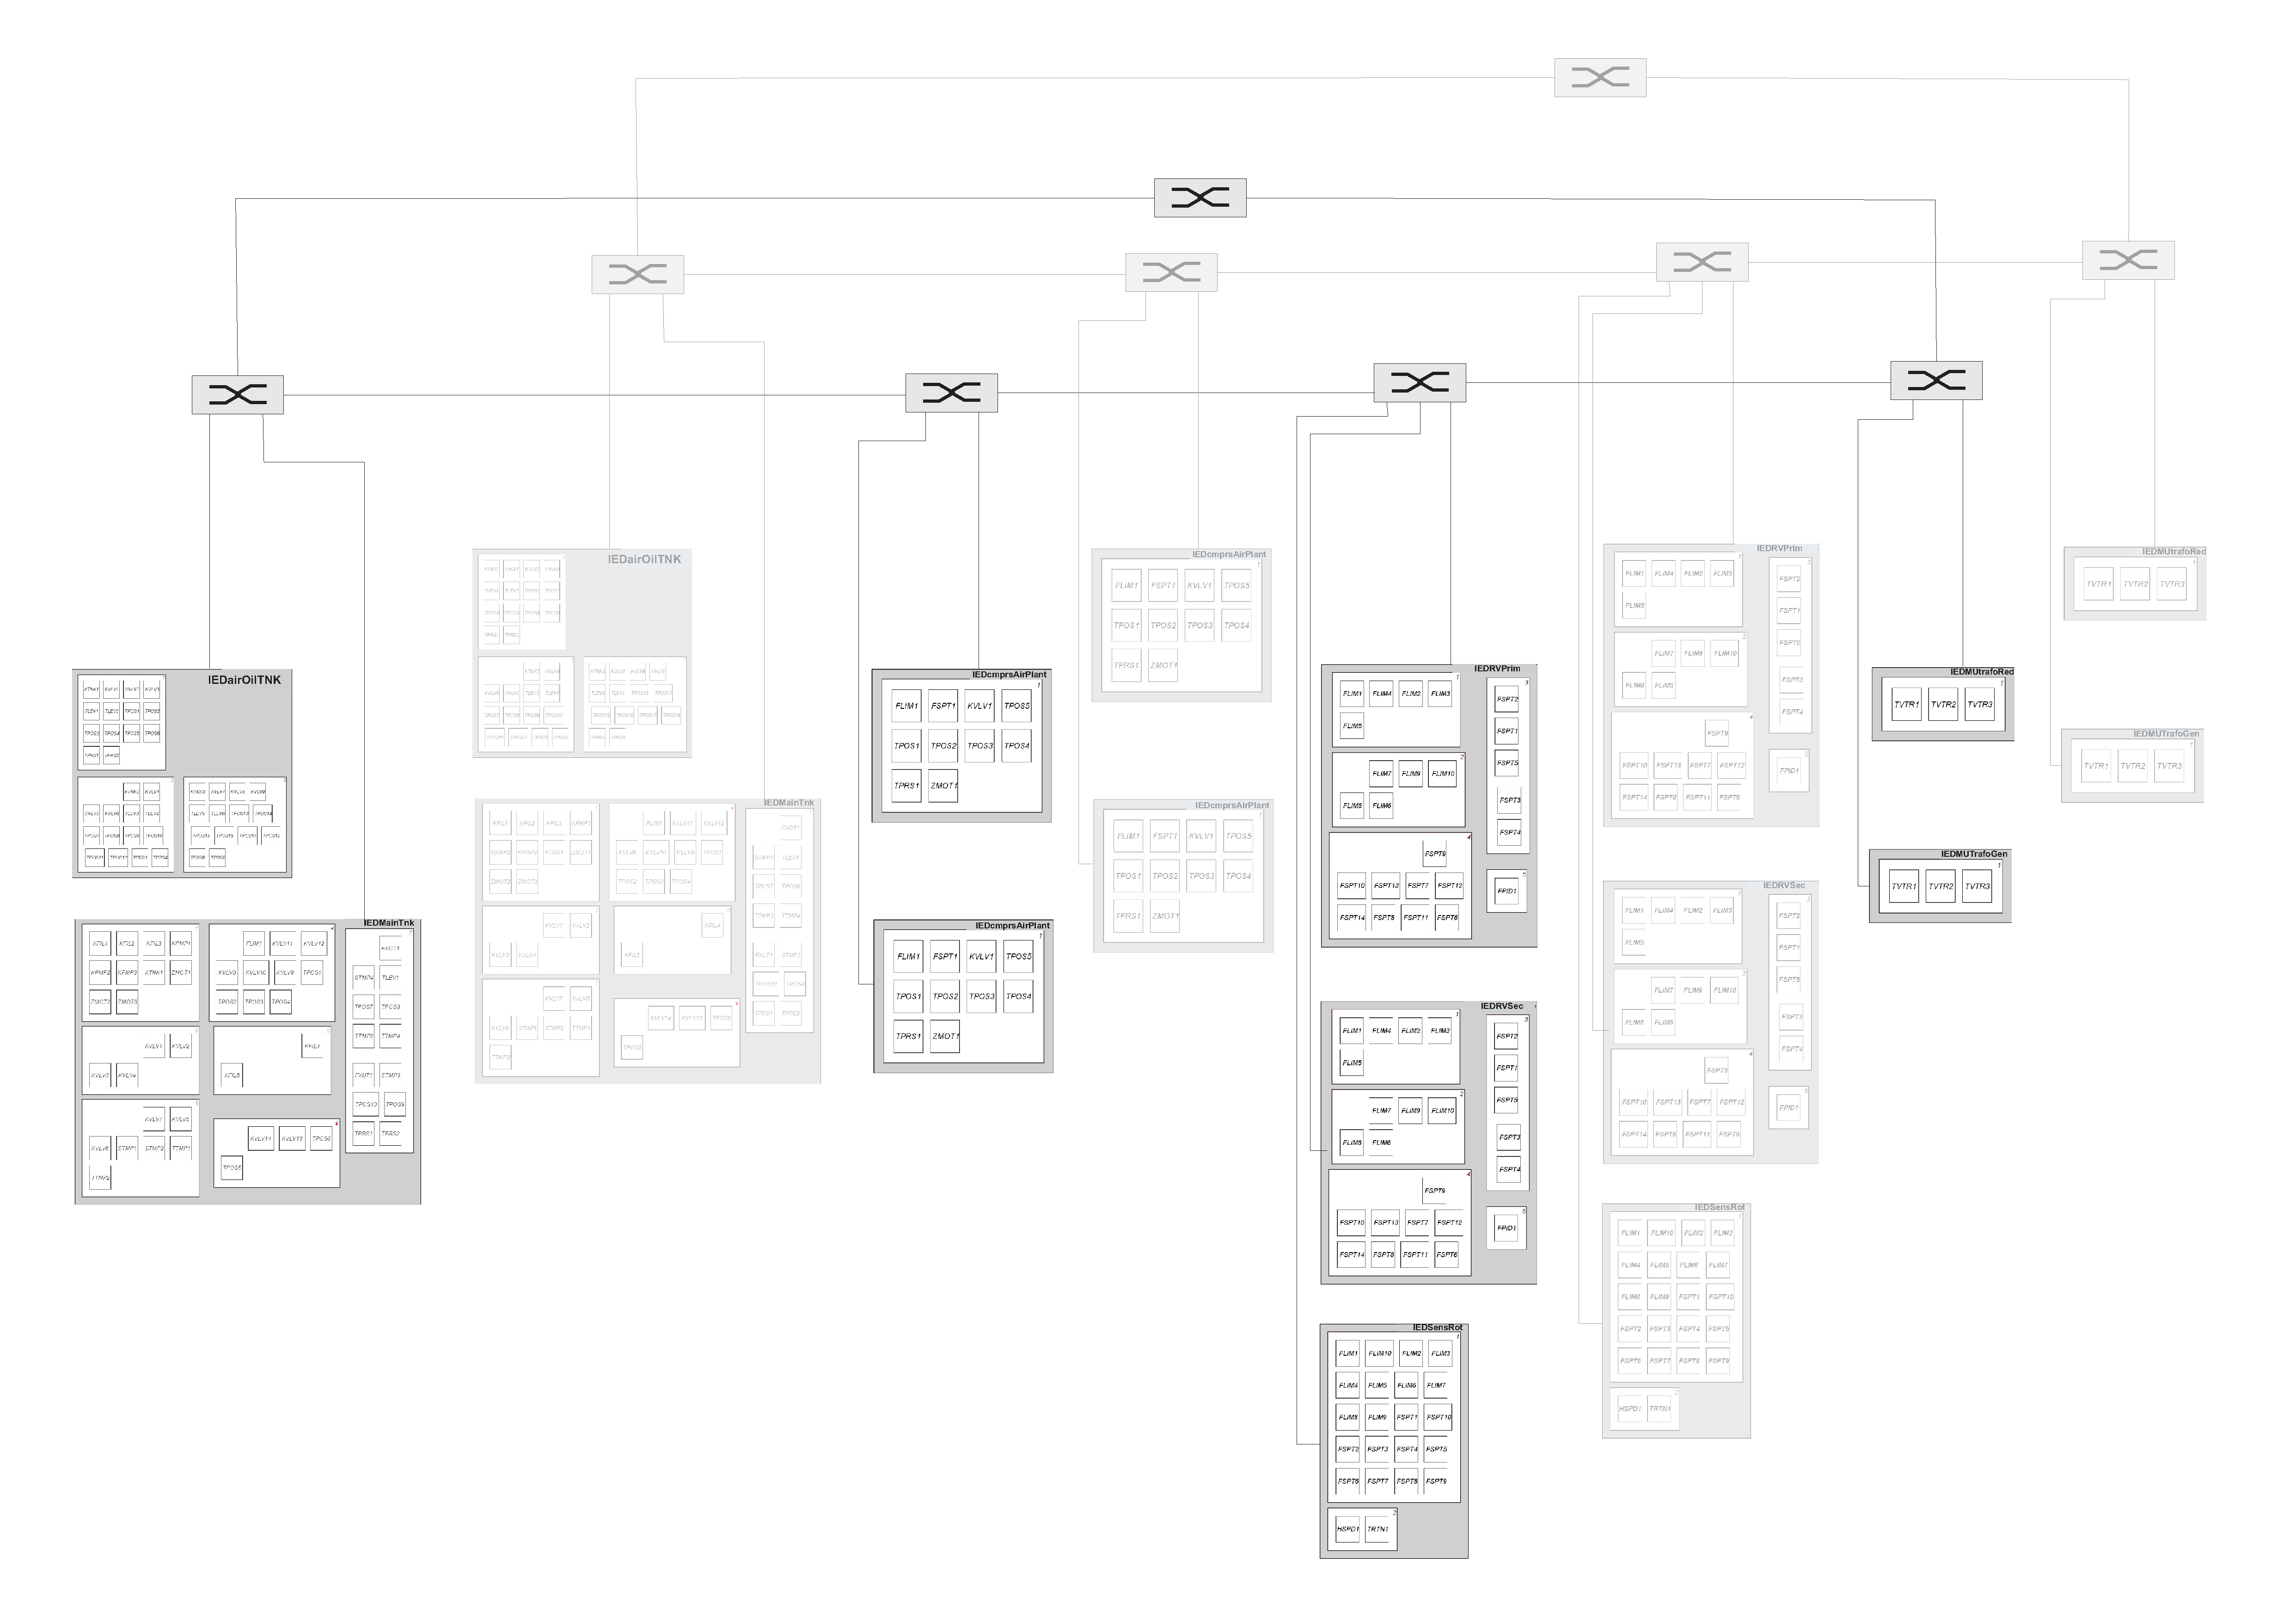
\includegraphics[width=1.0\linewidth]{chapters/model/figures/nodosLogicosDelSistema.eps} 
  \captionsetup{font=scriptsize}
  \caption{Resumen de los nodos l�gicos del regulador de velocidad ubicados seg�n la arquitectura referencial de la figura \ref{fig:arquitectura-Gral-Referencial1} }
  \label{fig:LNodes-reg-veloc}
\end{center}
\end{figure}
\end{landscape}



\section{Servicios de comunicaci�n}

El modelo de los servicios de comunicaci�n de los IEDs definidos en este trabajo
son presentados a trav�s de la variante SCL ISNP (secci�n \ref{sec:ied-simplificado-y-no-pre-configurado}), conforme al proceso de ingenier�a
definido en el cap�tulo \ref{ch:enfoque-del-autor}.

En las siguientes subsecciones se presenta la descripci�n del modelo de servicios ACSI 
utilizando una notaci�n simple y amigable para el lector (formato tabla). Las definiciones 
formales, presentadas en SCL, pueden ser encontradas en el ap�ndice \ref{app:resultados2-codigos-SCL}.
 

\subsection{Servicios ACSI de los IEDs IEDRV, IEDMainTnk, IEDairOilTNK e IEDcmprsAirPlant}

    \begin{table}[H]
	\begin{center}    
	\begin{tabular}{|l|p{8cm}|}
	    \hline
	    \multicolumn{2}{|c|}{\cellcolor[gray]{0.8}  \textbf{IED IEDRV - Servicios ACSI}  } \\
	        \hline
	        \textbf{Nombre del Servicio ACSI} & \textbf{Par�metros del servicio} \\
	        \hline 
	        DynAssociation &  \\
	        \hline
	        GetDataObjectDefinition &  \\
	        \hline
	        DataObjectDirectory &  \\
	        \hline
	        GetDataSetValue &  \\
	        \hline
	        SetDataSetValue &  \\
	        \hline
	        DataSetDirectory &  \\
	        \hline
	        ConfDataSet & max=50, maxAttributes=250 \\
	        \hline
	        GetDirectory &  \\
	        \hline
	        ReadWrite &  \\
	        \hline
	        ConfReportControl & max=7 \\
	        \hline
	        GetCBValues &  \\
	        \hline
	        ReportSettings & intgPd=Dyn, trgOps=Dyn, bufTime=Dyn, optFields=Dyn, rptID=Dyn, datSet=Fix, cbName=Fix \\
	        \hline
	        GSESettings & appID=Fix, cbName=Fix, dataLabel=Dyn, datSet=Fix \\
	        \hline
	        GOOSE & max=5 \\
	        \hline
	        FileHandling &  \\
	        \hline
	        ConfLNs & fixLnInst=true, fixPrefix=false \\
	        \hline
			SMVSettings & smpRate=Conf \\
	        \hline
	\end{tabular}
    \caption{Servicios ACSI de los IEDs IEDRV, IEDMainTnk, IEDairOilTNK e IEDcmprsAirPlant}
    \label{table:app-Servicios-acsi-IEDs}
	\end{center}
    \end{table}

%\subsection{Servicios ACSI del IED IEDMainTnk}
%\subsection{Servicios ACSI del IED IEDairOilTNK}
%\subsection{Servicios ACSI del IED IEDcmprsAirPlant}

\subsection{Servicios ACSI del IED IEDsensRot}

    \begin{table}[H]
	\begin{center}    
	\begin{tabular}{|l|p{8cm}|}
	    \hline
	    \multicolumn{2}{|c|}{\cellcolor[gray]{0.8}  \textbf{IED IEDMainTnk - Servicios ACSI}  } \\
	        \hline
	        \textbf{Nombre del Servicio ACSI} & \textbf{Par�metros del servicio} \\
	        \hline
	        GetDataObjectDefinition &  \\
	        \hline
	        DataObjectDirectory &  \\
	        \hline
	        DataSetDirectory &  \\
	        \hline
	        ConfDataSet & max=5, maxAttributes=50 \\
	        \hline
	        GetDirectory &  \\
	        \hline
	        ConfReportControl & max=5 \\
	        \hline
	        GetCBValues &  \\
	        \hline
	        ReportSettings & intgPd=Dyn, trgOps=Dyn, bufTime=Dyn, optFields=Dyn, rptID=Dyn, datSet=Fix, cbName=Fix \\
	        \hline
	        GSESettings & appID=Fix, cbName=Fix, dataLabel=Dyn, datSet=Fix \\
	        \hline
	        GOOSE & max=5 \\
	        \hline
	        FileHandling &  \\
	        \hline
	        ConfLNs & fixLnInst=true, fixPrefix=false \\
	        \hline
			SMVSettings & smpRate=Conf \\
	        \hline
	\end{tabular}
    \caption{Servicios ACSI para el IEDsensRot}
    \label{table:app-Servicios-acsi-IEDsensRot}
	\end{center}
    \end{table}


  
\chapter{Conclusiones}
\label{ch:conclusiones}
%\todo{completar las conclusiones!}

\section{Conclusiones}

Este Trabajo Final de Grado comienza 
en el cap�tulo \ref{ch:introduction} 
con una breve introducci�n a la norma IEC 61850. Esta 
introducci�n describe
la importancia de la norma, 
las nociones b�sicas de la 
norma, 
su aplicaci�n en las hidroel�ctricas, 
dando mayor enfoque a la explicaci�n del 
modelo de informaci�n y servicios que ofrece 
la IEC 61850, y a la explicaci�n del 
lenguaje de configuraci�n de estos 
sistemas de comunicaci�n y redes.

Un objetivo importante de este trabajo 
es interpretar la norma IEC 61850, 
identificando sus puntos fuertes y d�biles
para su aplicaci�n en centrales hidroel�ctricas. 
Acorde a esto, en los cap�tulos 
\ref{cap:planteamiento-del-problema} y
\ref{ch:enfoque-del-autor}
se identificaron los problemas y los desaf�os 
existentes durante el proceso de ingenier�a IEC 61850
en sistemas de automatizaci�n de centrales hidroel�ctricas,
dando un primer paso en la armonizaci�n de 
la IEC 61850 con la IEEE 830 \cite{IEEE:830-1998}, 
y visualizando 
las ventajas que tendr�a la adaptaci�n y
aplicaci�n de esta norma IEEE
para la identificaci�n de los requisitos 
que deben cumplir los sistemas IEC 61850
a ser dise�ados en una forma totalmente sistem�tica,
y se explica al lector el enfoque adoptado por el 
autor de este trabajo durante
todo el proceso de ingenier�a correspondiente
a los objetivos del trabajo. La investigaci�n
descripta en el cap�tulo 
\ref{ch:enfoque-del-autor}
ha mejorado la comprensi�n de la norma 
IEC 61850, en especial del proceso de 
ingenier�a produce resultados en 
el formato formal 
definido en IEC 61850--6 \cite{IEC61850-6:2004}.
Un an�lisis del uso de ICDs para 
especificaci�n de equipamientos IEC 61850 
ha sido profundizado, ofreciendo 
datos y ejemplos concretos, describiendo 
sus ventajas y desventajas.

De esta manera, en el cap�tulo \ref{cap:model}
se aborda el objetivo principal de este trabajo: 
El dise�o del modelo IEC 61850 del regulador de velocidad 
de una unidad generadora t�pica de la 
Central Hidroel�ctrica Itaipu. Este  
dise�o se realiza aplicando el enfoque
propuesto en el proceso de ingenier�a  
explicado en el cap�tulo 
\ref{ch:enfoque-del-autor}.
En este cap�tulo se propone la inclusi�n
de dos nodos l�gicos a la norma IEC 61850,
de modo a enriquecer e ir cubriendo todas 
las necesidades del \gls{SAS}, 
y en las secciones \ref{sec:LNs-del-IEDRV}
en adelante se gener� en forma autom�tica
acorde a las directrices de la norma IEC 61346,
descriptas en la secci�n \ref{sec:doc-automatica}, 
tomando como informaci�n estructurada el 
resultado del dise�o, que se present� 
en formato SCL en el 
anexo \ref{app:resultados2-codigos-SCL}.

%\section{Sumario de contribuciones}

\section{Futuros trabajos}

Esta secci�n discute las limitaciones de este 
trabajo, y en base a eso se formularon
posibles opciones de futura investigaci�n
para mejorar el dise�o y enfoque de dise�o 
propuesto en este trabajo.

Cuando se levantaron los requisitos del 
sistema en el 
cap�tulo \ref{cap:planteamiento-del-problema},
se hizo alusi�n a la aplicaci�n de 
la norma IEEE 830 \cite{IEEE:830-1998}
para el levantamiento de los requisitos
de un sistema IEC 61850. En este trabajo 
se ha hecho una aplicaci�n muy b�sica 
e incompleta de esta norma IEEE. Una
posible futura extensi�n de esta 
investigaci�n podr�a tratar la 
armonizaci�n (con suficiente nivel de detalle) de la 
IEC 61850 con la IEEE 830.

En el cap�tulo 
\ref{cap:model},
mucho c�digo fuente SCL ha sido escrito 
a mano (usando herramientas de edici�n
de archivos XML gen�ricas, no herramientas
de ingenier�a espec�ficas en la norma IEC 61850)
debido a que a la fecha de elaboraci�n 
de este trabajo las herramientas de ingenier�a 
disponibles en el mercado no cubr�an todas 
las necesidades requeridas para 
el proceso de ingenier�a adoptado 
en este trabajo. Un futuro trabajo de 
aqu� a un par de a�os, podr�a 
rever las opciones existentes en el 
mercado para identificar las herramientas
de ingenier�a espec�ficas para la norma 
IEC 61850, considerando que 
dichas herramientas a�n se encuentran 
en sus primeras versiones estables, y
est�n evolucionando muy r�pidamente.


El autor de este
trabajo tiene entendido que los documentos oficiales que describen aspectos relevantes 
del  dise�o de modelos de sistemas IEC 61850 para hidroel�ctricas est�n en proceso
de elaboraci�n, y ser�n publicados en breve bajo la serie IEC 61850--7--510
\cite{IEC61850-7-510:2009}.
En base a esos documentos, 
ser� posible adaptar el enfoque planteado en este 
trabajo a las directrices dadas por la IEC en dichos documentos, y tambi�n 
ser� posible proponer la adopci�n, en parte,  
del enfoque planteado en este trabajo 
en las siguientes ediciones de los 
documentos de la IEC mencionados arriba, 
en caso de que sea oportuno. Esto 
constituye todo un trabajo de investigaci�n 
que podr�a realizarse en el futuro.


Como otra opci�n de trabajo futuro, tambi�n
se ha identificado la 
pertinencia de iniciar los estudios
para desarrollar herramientas de ingenier�a hechas a
medida de las necesidades particulares de un usuario.

En este trabajo no se han levantado los requisitos 
de comunicaci�n utilizando el enfoque PICOM definido 
en el apartado IEC 61850--5 \cite{IEC61850-5:2003}. 
Es muy importante aplicar el enfoque PICOM 
a los dise�os de modelos IEC 61850 debido 
a que permiten definir los servicios de comunicaci�n m�s 
adecuados para el sistema, en base a los requisitos.
Un futuro trabajo podr�a ser la aplicaci�n del 
enfoque PICOM para la obtenci�n de un modelo 
IEC 61850 robusto.




  

\begin{singlespace} 
	%esta es la bibliografia standard de la IEEE
	\bibliographystyle{IEEEtran} %otra opci�n es 	%\bibliographystyle{plain}
	\bibliography{IEEEabrv,bibliography/myIEEEbibliography}
%	\bibliographystyle{plain}
\end{singlespace}

\appendix 
%\chapter{Tables}

\begin{table}
\caption{Armadillos}
\label{arm:table}
\begin{center}
\begin{tabular}{||l|l||}\hline
Armadillos & are \\\hline
our	   & friends \\\hline
\end{tabular}
\end{center}
\end{table}

\clearpage
\newpage

%\chapter{Figures}

\vspace*{-3in}

\begin{figure}
\vspace{2.4in}
\caption{Armadillo slaying lawyer.}
\label{arm:fig1}
\end{figure}
\clearpage
\newpage

\begin{figure}
\vspace{2.4in}
\caption{Armadillo eradicating national debt.}
\label{arm:fig2}
\end{figure}
\clearpage
\newpage


%este no funciona! no se que le pasa a
% los XMLS, posiblemente es problema de los encodings,
%por eso pase a pdf los xmls separadamente, y luego
%reci�n le anex� a el documento principal 
%\chapter{Resultados del trabajo, en formato SCL}
\label{app:resultados-codigos-SCL}


\section{ICD del regulador de velocidad (regulaci�n primaria)}
\lstinputlisting[label=cod:ICD-IED_RV-primaria-xml,
caption=ICD de la regulaci�n primaria]
{governorModel/ICDs/IED_RV.xml} 

\section{ICD del regulador de velocidad (regulaci�n secundaria)}
\todo{actualizar urgente!}
\lstinputlisting[label=cod:ICD-IED_RV-secundaria-xml,
caption=ICD de la regulaci�n secundaria]
{governorModel/ICDs/IED_RV.xml} 

\section{ICD del sensor de rotaci�n}
\lstinputlisting[label=cod:ICD-sensor-rotacion-xml,
caption=ICD del sensor de rotaci�n]
{governorModel/ICDs/IED_rot_sensor.xml} 

\section{ICD del tanque principal}
\lstinputlisting[label=cod:ICD-IED_MAIN_TNK-xml,
caption=ICD del tanque principal]
{governorModel/ICDs/IED_MAIN_TNK.xml} 

\section{ICD de la planta a aire comprimido}
\lstinputlisting[label=cod:ICD-IED_compressed_air_plant-xml,
caption=ICD del compresor de aire]
{governorModel/ICDs/IED_compressed_air_plant.xml} 

\section{ICD del tanque de compresi�n de aire y de aceite}
\lstinputlisting[label=cod:ICD-IED_air-oil_PRS_TNK-xml,
caption=ICD del tanque de compresi�n de aire y de aceite]
{governorModel/ICDs/IED_air-oil_PRS_TNK.xml} 
 
\chapter{Resultados del trabajo, en formato SCL}
\label{app:resultados2-codigos-SCL}


\newpage
\vspace*{\fill}
	\begingroup
\section{ICD del regulador de velocidad (regulaci�n primaria)}
	\endgroup
\vspace*{\fill}
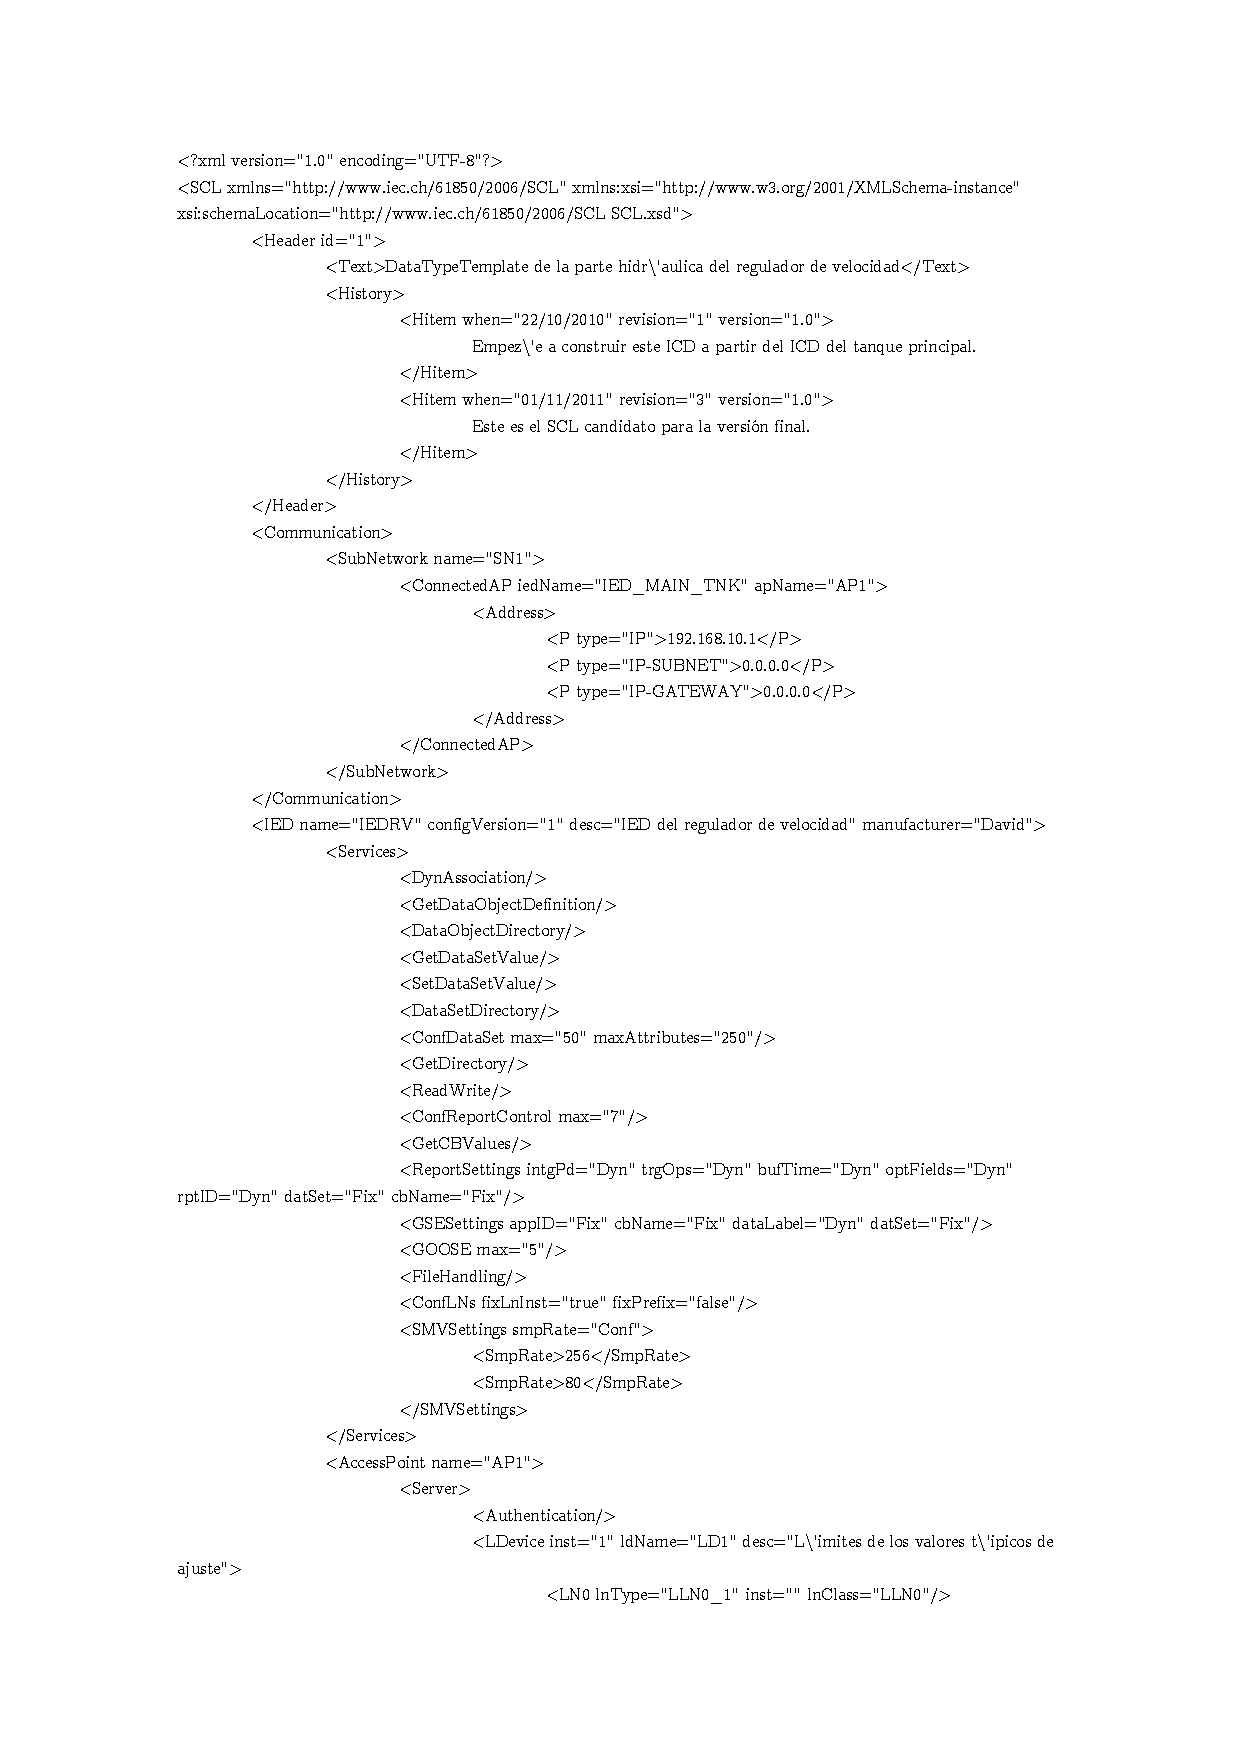
\includepdf[pages=1-4]{appendices/ICD-IED_RV.pdf} 
%\lstinputlisting[label=cod:ICD-IED_RV-primaria-xml,
%caption=ICD de la regulaci�n primaria]
%{governorModel/ICDs/IED_RV.xml} 



\vspace*{\fill}
	\begingroup
\section{ICD del regulador de velocidad (regulaci�n secundaria)}
	\endgroup
\vspace*{\fill}
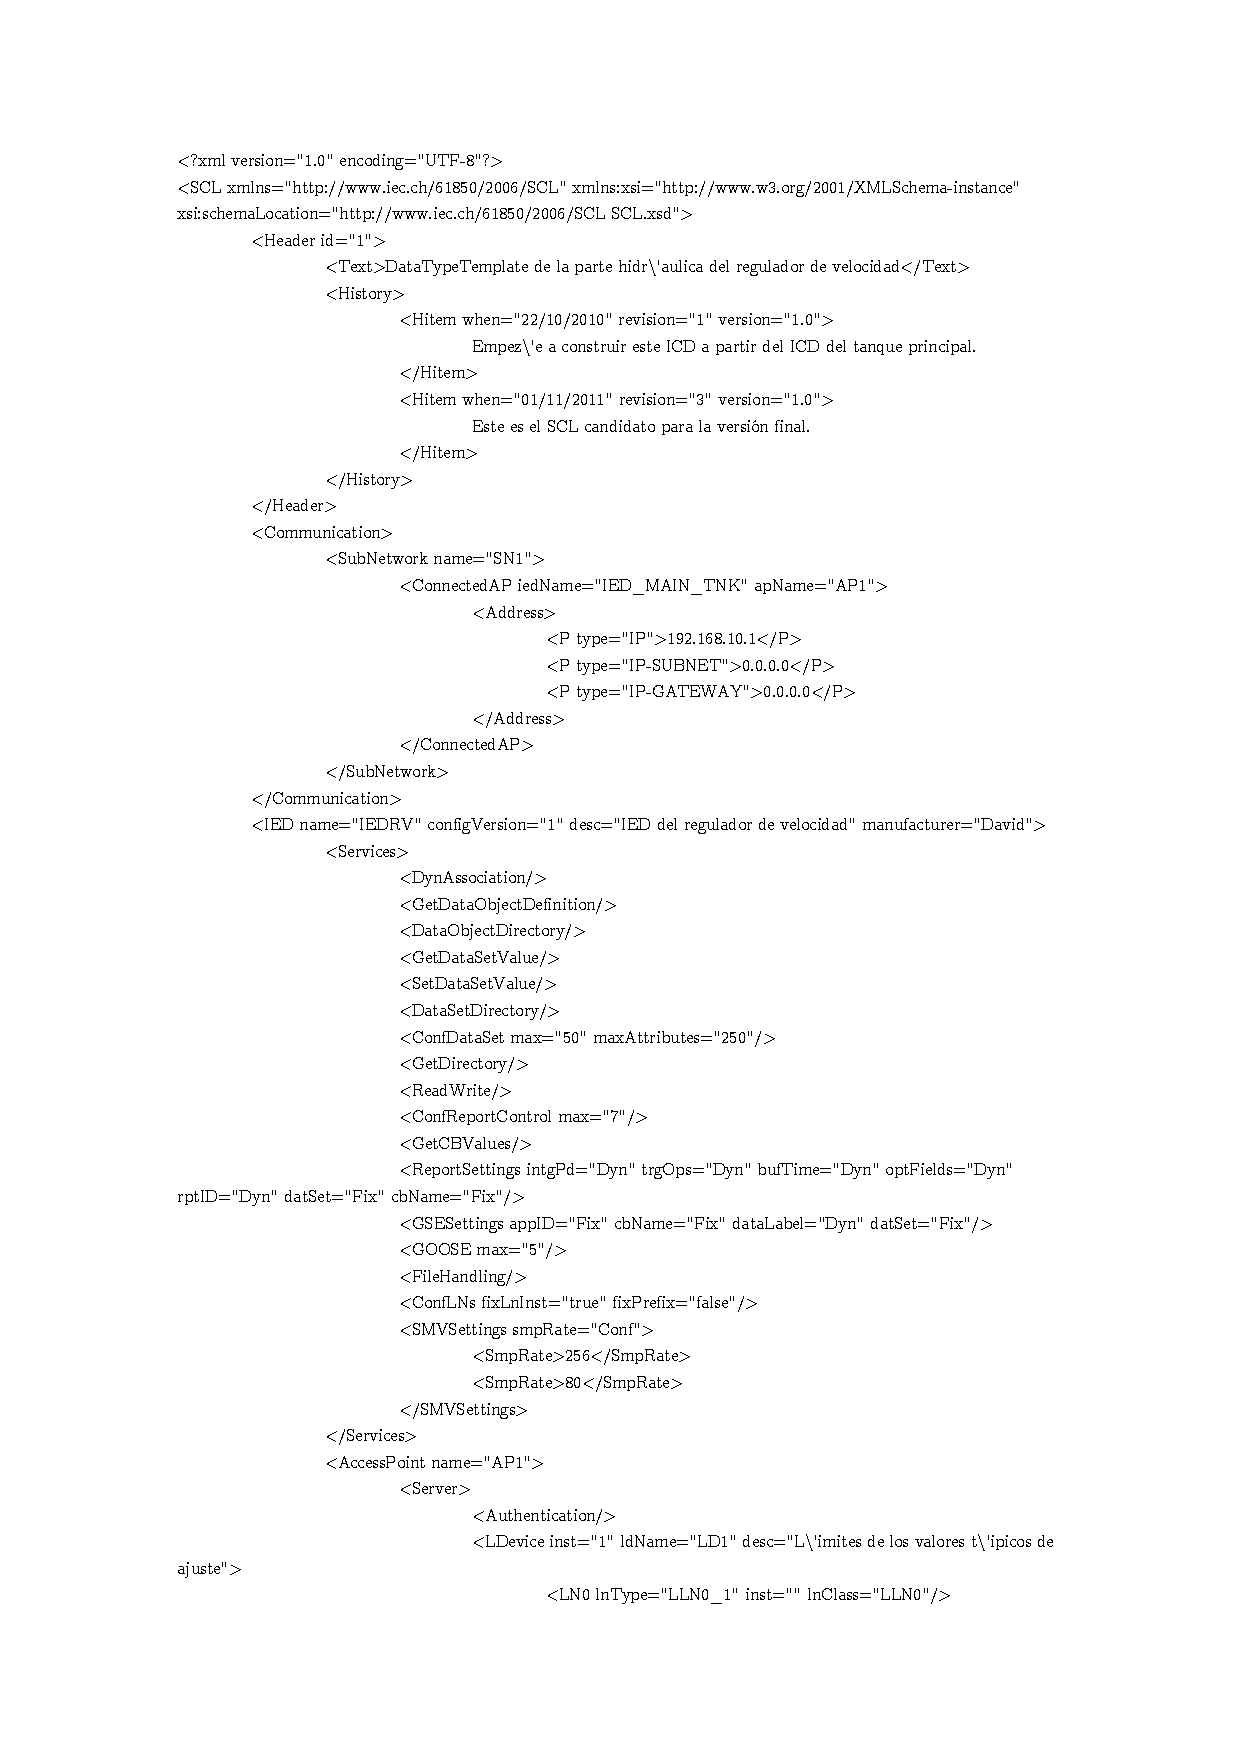
\includepdf[pages=1-4]{appendices/ICD-IED_RV.pdf} 


\vspace*{\fill}
	\begingroup
\section{ICD del sensor de rotaci�n}
	\endgroup
\vspace*{\fill}
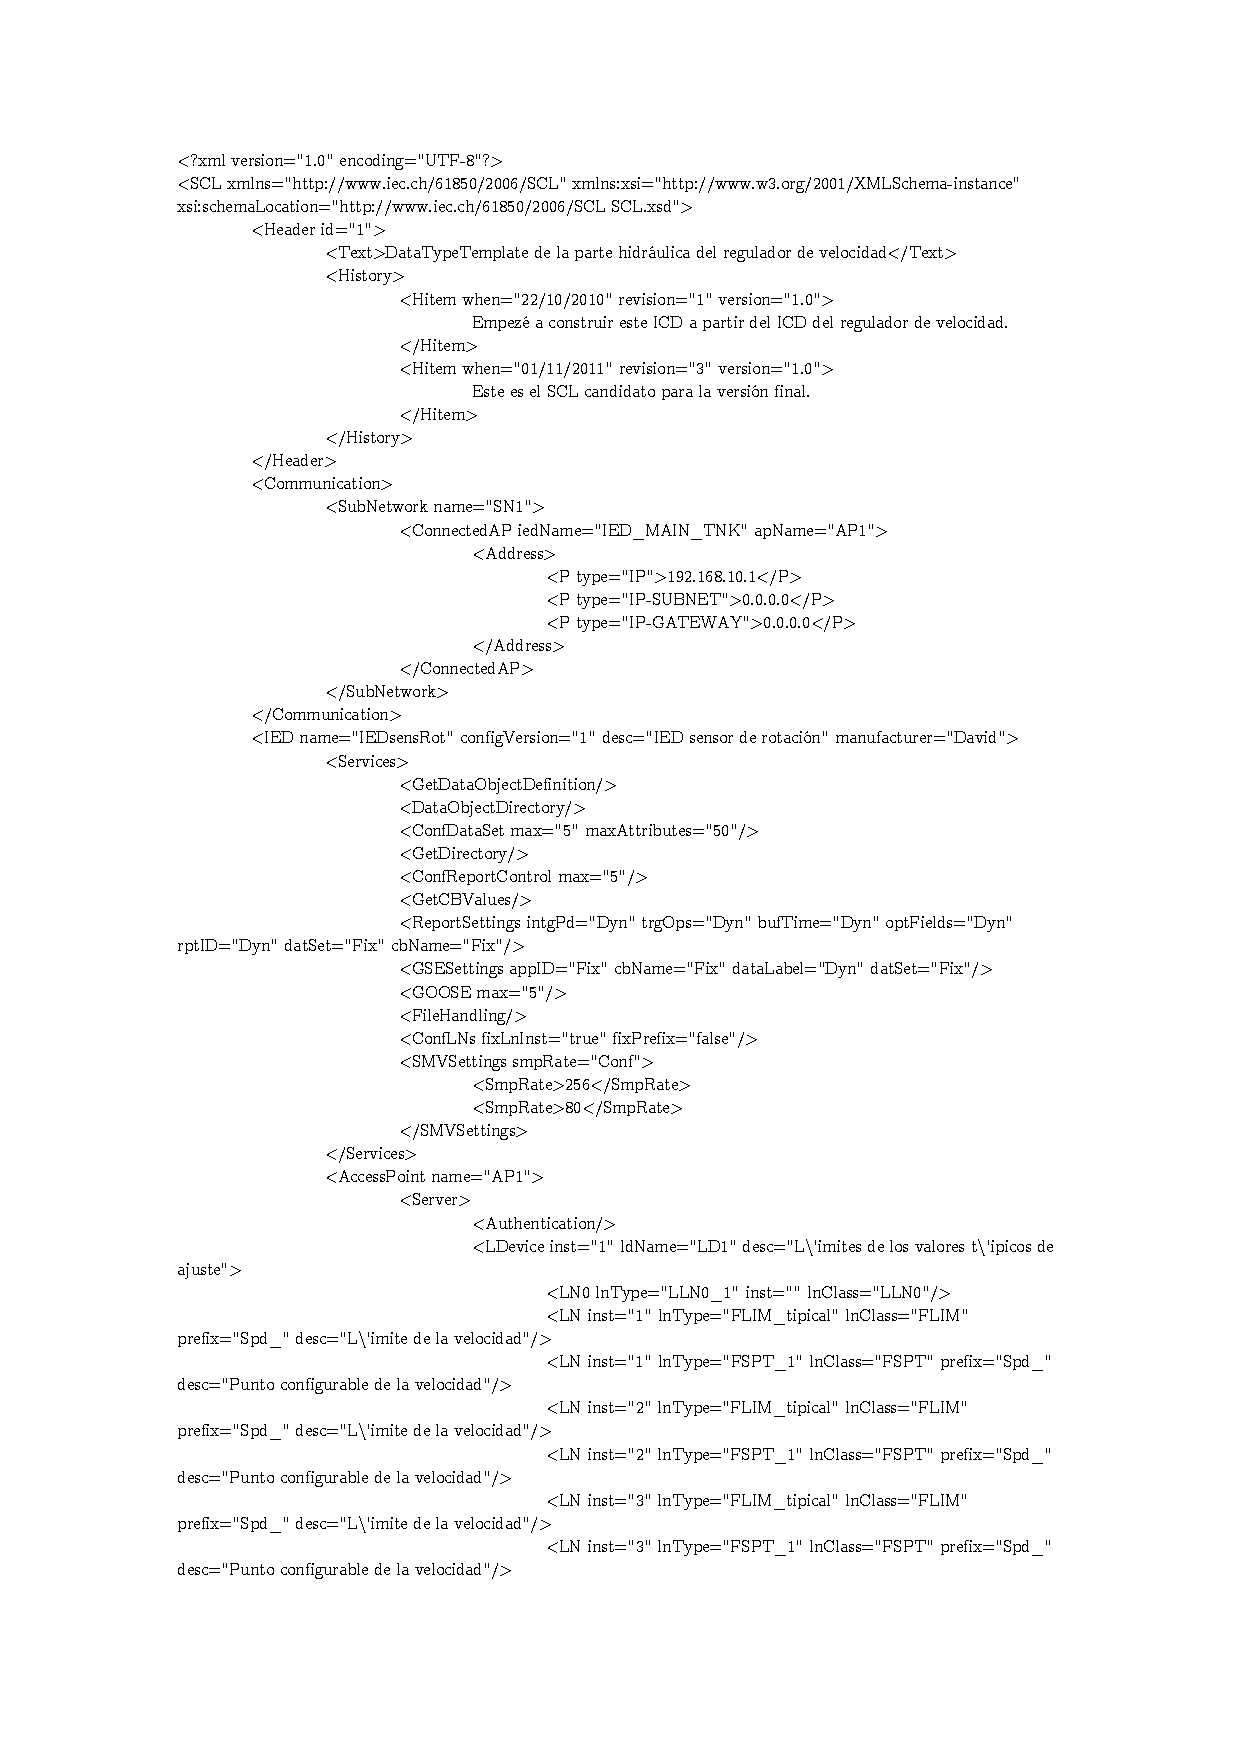
\includepdf[pages=1-4]{appendices/ICD-IED_rot_sensor.pdf} 


\vspace*{\fill}
	\begingroup
\section{ICD del tanque principal}
	\endgroup
\vspace*{\fill}
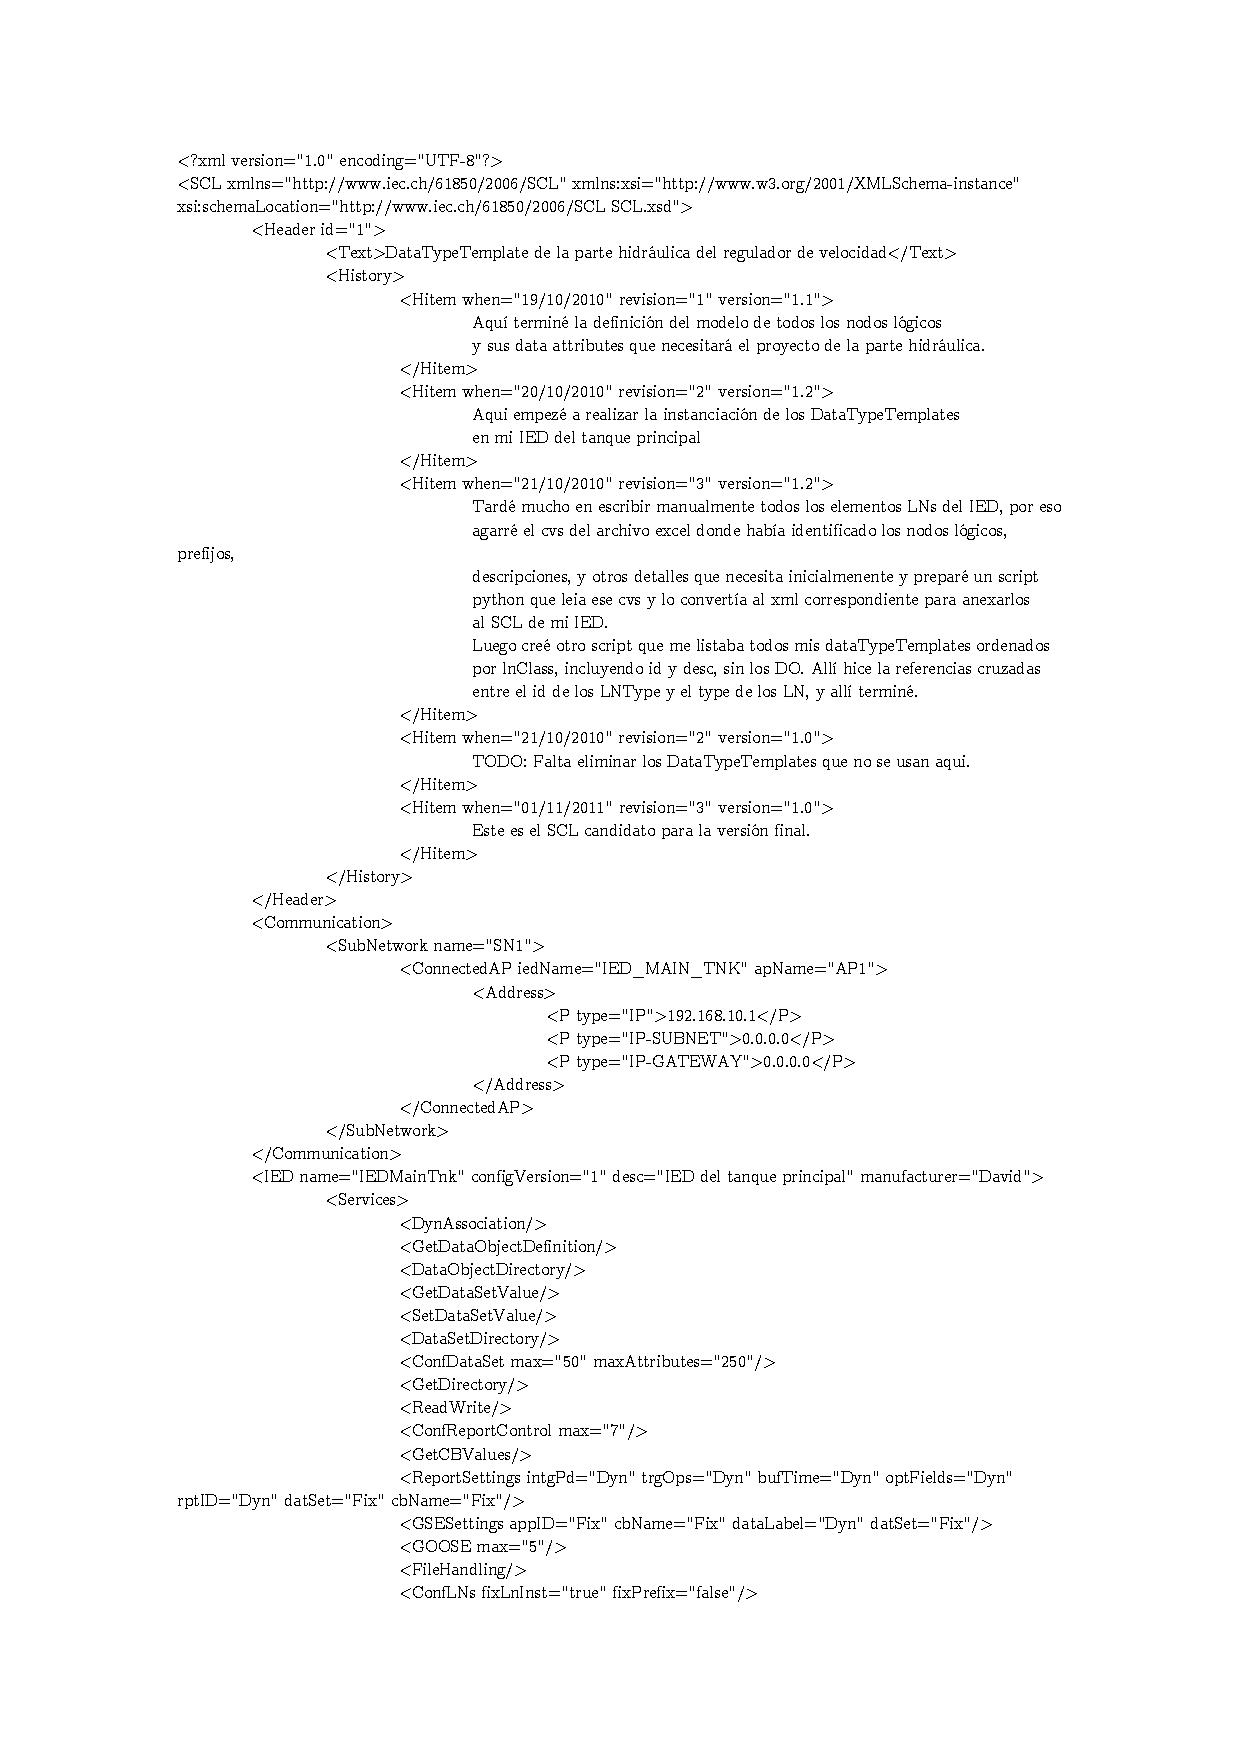
\includepdf[pages=1-11]{appendices/ICD-IED_MAIN_TNK.pdf} 



\vspace*{\fill}
	\begingroup
\section{ICD de la planta a aire comprimido}
	\endgroup
\vspace*{\fill}
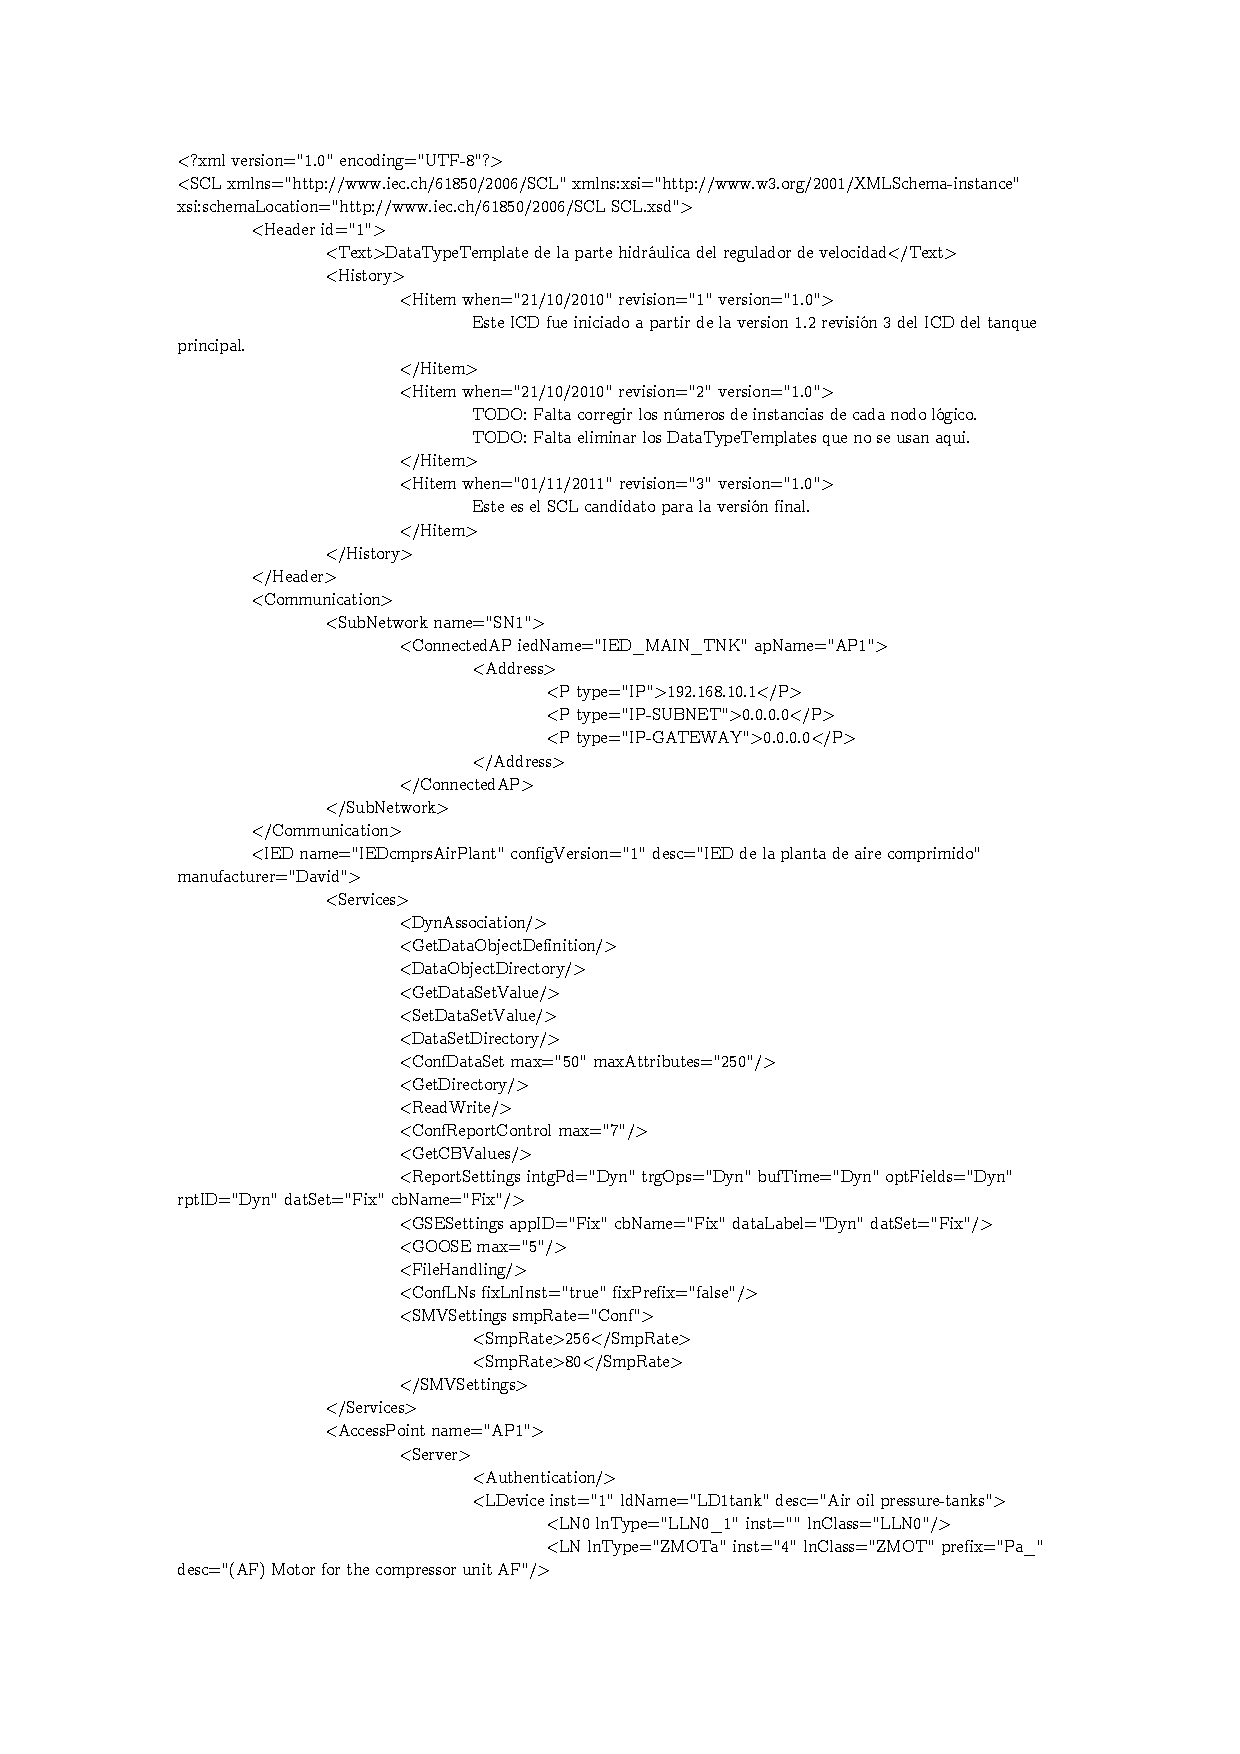
\includepdf[pages=1-4]{appendices/ICD-IED_compressed_air_plant.pdf} 



\vspace*{\fill}
	\begingroup
\section{ICD del tanque de compresi�n de aire y de aceite}
	\endgroup
\vspace*{\fill}
\includepdf[pages=1-6]{appendices/ICD-IED_air-oil_PRS_TNK.pdf} 
  



\vspace*{\fill}
	\begingroup
\section{SSD de todo el sistema}
	\endgroup
\vspace*{\fill}
\includepdf[pages=1-21]{appendices/SSD_MRV.pdf} 
  
  
 
\section{SCL XML Shemas modificados asociados a los ICDs del proyecto}

Para este trabajo se han utilizado los XML Shemas 
definidos en el apartado IEC 61850-6, edici�n 1 \cite{IEC61850-6:2004},
y se han realizado algunas modificaciones, 
proveidas en las secciones los c�digos fuente \ref{cod:scl-xsd} y
\ref{cod:SCL_Enums-xsd}, para agregar los nodos l�gicos 
para centrales hidroel�ctricas 
definidos en IEC 61850-7-410 \cite{IEC61850-7-410:2007}. En 
los dem�s ficheros \emph{XSD} s�lo se ha modificado
el espacio de nombres, que originalmente estaba
definido con la URL de 2006 en \cite{IEC61850-6:2004},
y en el presente trabajo se cambi� dicho espacio 
de nombres para la URL de 2003 de la iec, 
porque el la herramienta de ingenier�a Atlan61850
s�lo aceptaba este espacio de nombres. Con la herramienta
Atlan61850 fue obtenida la figura \ref{fig:LNodes-reg-veloc}
(y luego han sido retocados con otro software de prop�sito general 
para la edici�n de im�genes).

Est� claro que 
utilizar el fichero XSD 
\emph{SCL\_Maintenance} para 
realizar estas modificaciones
es una buena pr�ctica. Dicho 
enfoque ser� considerado por el autor para un 
trabajo futuro (los resultados son los mismos,
s�lo cambia la modularidad del c�digo fuente 
donde se encuentran las definciones).

	\subsection{SCL.xsd}
		\lstinputlisting[label=cod:scl-xsd,
		caption=SCL.xsd]
		{governorModel/xsd2003/SCL.xsd} 

	\subsection{SCL\_Enums.xsd}
		\lstinputlisting[label=cod:SCL_Enums-xsd,
		caption=SCL\_Enums.xsd]
		{governorModel/xsd2003/SCL_Enums.xsd} 


\chapter{Archivos SCL complementarios}
\label{app:codigos-SCL}


\section{Profundidad completa del 
elemento \emph{Substation}}

\lstinputlisting[label=cod:substation-profundo-xml,
caption=Elemento \emph{Substation} con profundidad completa]
{chapters/enfoque/source/scl/substation-profundo.xml} 



\section{Profundidad completa del 
elemento \emph{IED}}
\label{app:SEC-profundidad-completa-IED}

\lstinputlisting[label=cod:ied-profundo-xml,
caption=Elemento \emph{IED} con profundidad completa]
{chapters/enfoque/source/scl/ied-profundo.xml} 

\chapter{Datos estad�siticos de ICDs disponibles en el mercado}

En este ap�ndice se muestran las estad�sticas de 
aspectos relevantes de 178 ICDs correspondientes 
a IEDs de 5 fabricantes. Estos ICDs se han obtenido en noviembre del 2010, y no se ha incluido 
ning�n ICD ficticio.  

Utilizando los 178 ICDs se pudo crear una 
base de datos de ICDs.  
A trav�s del lenguaje de programaci�n \emph{Python 2.6} 
el autor de este trabajo ha consultado la base de datos, y ha 
generado las tablas que se
visualizan en este cap�tulo.

\section{Servicios de comunicaci�n disponibles en el la base de datos}
	\label{app:Estadisticas-servicios}
	
    \begin{table}[H]
	\begin{center}    
	\begin{tabular}{|l|l|}
	    \hline
	    \multicolumn{2}{|c|}{\cellcolor[gray]{0.8} \textbf{IED - Servicios implementados en el mercado}  } \\
	        \hline
	        \textbf{Servicio ACSI} & \textbf{Cantidad de IEDs que lo implementan} \\
	        \hline 
	        GetDirectory & 178 \\
	        \hline
	        ConfReportControl & 63 \\
	        \hline
	        FileHandling & 119 \\
	        \hline
	\end{tabular}
    \caption{Servicios implementados en el mercado}
    \label{table:app-Servicios-implementados-mercado1}
	\end{center}
    \end{table}



    \begin{table}[H]
	\begin{center}    
	\begin{tabular}{|l|l|}
	    \hline
	    \multicolumn{2}{|c|}{\cellcolor[gray]{0.8} \textbf{IED - Servicios implementados en el mercado}  } \\
	        \hline
	        \textbf{Servicio ACSI} & \textbf{Cantidad de IEDs que lo implementan} \\
	        \hline 
	        GSSE & 1 \\
	        \hline
	        ConfDataSet & 156 \\
	        \hline
	        GetDataSetValue & 178 \\
	        \hline
	        SetDataSetValue & 59 \\
	        \hline
	        GetCBValues & 178 \\
	        \hline
	        ReadWrite & 178 \\
	        \hline
	        GetDataObjectDefinition & 178 \\
	        \hline
	        ConfLNs & 175 \\
	        \hline
	        DataSetDirectory & 177 \\
	        \hline
	        TimerActivatedControl & 1 \\
	        \hline
	        ReportSettings & 177 \\
	        \hline
	        DynAssociation & 178 \\
	        \hline
	        GSEDir & 1 \\
	        \hline
	        ConfLogControl & 1 \\
	        \hline
	        DynDataSet & 2 \\
	        \hline
	        GOOSE & 177 \\
	        \hline
	        DataObjectDirectory & 178 \\
	        \hline
	        GSESettings & 173 \\
	        \hline
	\end{tabular}
    \caption{Servicios implementados en el mercado}
    \label{table:app-Servicios-implementados-mercado2}
	\end{center}
    \end{table}


\section{Nodos l�gicos disponibles en la base de datos}


    \begin{table}[H]
	\begin{center}    
	\begin{tabular}{|l|l|}
	    \hline
	    \multicolumn{2}{|c|}{\cellcolor[gray]{0.8} \textbf{IED - Nodos l�gicos implementados en el mercado}  } \\
	        \hline
	        \textbf{LNClass} & \textbf{Cantidad de instancias encontradas en la base de datos} \\
	        \hline 
	        ZMOT & 2 \\
	        \hline
	        RADR & 15 \\
	        \hline
	        POPF & 22 \\
	        \hline
	        CSWI & 343 \\
	        \hline
	        PTUC & 50 \\
	        \hline
	        RDIR & 151 \\
	        \hline
	        RDRE & 121 \\
	        \hline
	        PHAR & 65 \\
	        \hline
	        SCBC & 1 \\
	        \hline
	        GAIO & 4 \\
	        \hline
	        PZSU & 10 \\
	        \hline
	        PFRC & 205 \\
	        \hline
	        CILO & 123 \\
	        \hline
	        RCCF & 1 \\
	        \hline
	        PDCF & 1 \\
	        \hline
	        PSOF & 94 \\
	        \hline
	        ZAXN & 6 \\
	        \hline
	        TVTR & 2 \\
	        \hline
	        RCLP & 1 \\
	        \hline
	        RFLO & 91 \\
	        \hline
	        RBRF & 266 \\
	        \hline
	        PTUF & 392 \\
	        \hline
	        MSQI & 210 \\
	        \hline
	\end{tabular}
    \caption{Nodos l�gicos implementados en el mercado}
    \label{table:app-LNs-implementados-mercado1}
	\end{center}
    \end{table}

    \begin{table}[H]
	\begin{center}    
	\begin{tabular}{|l|l|}
	    \hline
	    \multicolumn{2}{|c|}{\cellcolor[gray]{0.8} \textbf{IED - Nodos l�gicos implementados en el mercado}  } \\
	        \hline
	        \textbf{LNClass} & \textbf{Cantidad de instancias encontradas en la base de datos} \\
	        \hline
	        PIOC & 783 \\
	        \hline
	        MMTR & 37 \\
	        \hline
	        MTHE & 10 \\
	        \hline
	        MSTA & 238 \\
	        \hline
	        PVOC & 6 \\
	        \hline
	        PPWR & 20 \\
	        \hline
	        RCLI & 20 \\
	        \hline
	        GGIO & 2521 \\
	        \hline
	        PEFI & 3 \\
	        \hline
	        PTUV & 451 \\
	        \hline
	        XSWI & 368 \\
	        \hline
	        LPHD & 846 \\
	        \hline
	        PHIZ & 2 \\
	        \hline
	        XCBR & 325 \\
	        \hline
	        RTTR & 40 \\
	        \hline
	        MMOT & 1 \\
	        \hline
	        PSDE & 20 \\
	        \hline
	        MDIF & 3 \\
	        \hline
	        PLMP & 1 \\
	        \hline
	        PDUP & 122 \\
	        \hline
	        SIMG & 6 \\
	        \hline
	        XBCF & 1 \\
	        \hline
	        PTOV & 785 \\
	        \hline
	        RREC & 72 \\
	        \hline
	        PDIF & 278 \\
	        \hline
	\end{tabular}
    \caption{Nodos l�gicos implementados en el mercado}
    \label{table:app-LNs-implementados-mercado2}
	\end{center}
    \end{table}

    \begin{table}[H]
	\begin{center}    
	\begin{tabular}{|l|l|}
	    \hline
	    \multicolumn{2}{|c|}{\cellcolor[gray]{0.8} \textbf{IED - Nodos l�gicos implementados en el mercado}  } \\
	        \hline
	        \textbf{LNClass} & \textbf{Cantidad de instancias encontradas en la base de datos} \\
	        \hline 
	        TCTR & 3 \\
	        \hline
	        RVCS & 5 \\
	        \hline
	        YPTR & 1 \\
	        \hline
	        MTHR & 15 \\
	        \hline
	        PTTR & 211 \\
	        \hline
	        RBDR & 80 \\
	        \hline
	        PVPH & 46 \\
	        \hline
	        PMSS & 17 \\
	        \hline
	        PMRI & 27 \\
	        \hline
	        MMXU & 415 \\
	        \hline
	        PTAF & 24 \\
	        \hline
	        RPSB & 250 \\
	        \hline
	        PDMP & 3 \\
	        \hline
	        PDIS & 447 \\
	        \hline
	        PPAM & 3 \\
	        \hline
	        PTOF & 352 \\
	        \hline
	        PDOP & 126 \\
	        \hline
	        PTOC & 2657 \\
	        \hline
	        PTRC & 433 \\
	        \hline
	        CALH & 4 \\
	        \hline
	        RSYN & 95 \\
	        \hline
	        PSCH & 159 \\
	        \hline
	        MTHI & 13 \\
	        \hline
	        PVSP & 1 \\
	        \hline
	        MMXN & 91 \\
	        \hline
	\end{tabular}
    \caption{Nodos l�gicos implementados en el mercado}
    \label{table:app-LNs-implementados-mercado3}
	\end{center}
    \end{table}
	        
    \begin{table}[H]
	\begin{center}    
	\begin{tabular}{|l|l|}
	    \hline
	    \multicolumn{2}{|c|}{\cellcolor[gray]{0.8} \textbf{IED - Nodos l�gicos implementados en el mercado}  } \\
	        \hline
	        \textbf{LNClass} & \textbf{Cantidad de instancias encontradas en la base de datos} \\
	        \hline
	        PTEF & 20 \\
	        \hline
	        MTHM & 3 \\
	        \hline
	        MDST & 28 \\
	        \hline
	        ZBAT & 9 \\
	        \hline
	\end{tabular}
    \caption{Nodos l�gicos implementados en el mercado}
    \label{table:app-LNs-implementados-mercado4}
	\end{center}
    \end{table}
	
%\chapter{Implementaci�n del ACSI en Java}
\label{app:ACSI-implementation-in-java}
En este ap�ndice se presenta 
el c�digo fuente escrito por el autor 
de este trabajo utilizando el lenguaje 
de programaci�n Java.
Esta API escrita en Java no 
implementa todo el ACSI, es m�s,
no realiza una implementaci�n 
muy detallada ni precisa, 
tampoco sigue los patrones 
de dise�o ni las convencioens Java, 
simplemente  
fue desarrollado para comprender 
y analizar ciertos aspectos
de implementaci�n de la serie 
IEC 61850-7-x, intentando
realizar las implementaciones de 
la forma m�s aproximada a las 
definiciones de la norma IEC 61850.
Resulta claro de que una implementaci�n 
real del ACSI es mucho m�s compleja 
y detallada que la presentada 
en este cap�tulo. 


\lstinputlisting[label=cod:ACSIClass-java,
caption=ACSIClass]
{chapters/oop/source/java_ACSI/src/ACSI/informationModels/ACSIClass.java}

\lstinputlisting[label=cod:DATA-java,
caption=DATA]
{chapters/oop/source/java_ACSI/src/ACSI/informationModels/DATA.java}

\lstinputlisting[label=cod:LOGICALDEVICE-java,
caption=Logical Device]
{chapters/oop/source/java_ACSI/src/ACSI/informationModels/LOGICAL_DEVICE.java}

\lstinputlisting[label=cod:LOGICALNODELN0-java,
caption=Logical Node LN0]
{chapters/oop/source/java_ACSI/src/ACSI/informationModels/LOGICAL_NODE_LN0.java}

\lstinputlisting[label=cod:LOGICALNODEL-java,
caption=Logical Node]
{chapters/oop/source/java_ACSI/src/ACSI/informationModels/LOGICAL_NODE.java}

\lstinputlisting[label=cod:SERVER-java,
caption=Server]
{chapters/oop/source/java_ACSI/src/ACSI/informationModels/SERVER.java}

\lstinputlisting[label=cod:CompositeCDC-java,
caption=CompositeCDC]
{chapters/oop/source/java_ACSI/src/ACSI/informationModels/Data/CompositeCDC.java}

\lstinputlisting[label=cod:SimpleCDC-java,
caption=SimpleCDC]
{chapters/oop/source/java_ACSI/src/ACSI/informationModels/Data/SimpleCDC.java}

\lstinputlisting[label=cod:BasicType-java,
caption=BasicType]
{chapters/oop/source/java_ACSI/src/ACSI/informationModels/DataAttribute/BasicType.java}

\lstinputlisting[label=cod:CompositeComponent-java,
caption=CompositeComponent]
{chapters/oop/source/java_ACSI/src/ACSI/informationModels/DataAttribute/CompositeComponent.java}

\lstinputlisting[label=cod:DAType-java,
caption=DAType]
{chapters/oop/source/java_ACSI/src/ACSI/informationModels/DataAttribute/DAType.java}

\lstinputlisting[label=cod:Prescence-java,
caption=Prescence]
{chapters/oop/source/java_ACSI/src/ACSI/informationModels/DataAttribute/Prescence.java}

\lstinputlisting[label=cod:PrimitiveComponent-java,
caption=PrimitiveComponent]
{chapters/oop/source/java_ACSI/src/ACSI/informationModels/DataAttribute/PrimitiveComponent.java}

\lstinputlisting[label=cod:EntryTime-java,
caption=EntryTime]
{chapters/oop/source/java_ACSI/src/ACSI/informationModels/DataAttribute/common/EntryTime.java}

\lstinputlisting[label=cod:TimeQuality-java,
caption=TimeQuality]
{chapters/oop/source/java_ACSI/src/ACSI/informationModels/DataAttribute/common/TimeQuality.java}

\lstinputlisting[label=cod:TimeStamp-java,
caption=TimeStamp]
{chapters/oop/source/java_ACSI/src/ACSI/informationModels/DataAttribute/common/TimeStamp.java}

\lstinputlisting[label=cod:TriggerConditions-java,
caption=TriggerConditions]
{chapters/oop/source/java_ACSI/src/ACSI/informationModels/DataAttribute/common/TriggerConditions.java}

\lstinputlisting[label=cod:ASSOCIATION-java,
caption=ASSOCIATION]
{chapters/oop/source/java_ACSI/src/ACSI/informationModels/services/ASSOCIATION.java}

\lstinputlisting[label=cod:MCAA-java,
caption=MCAA]
{chapters/oop/source/java_ACSI/src/ACSI/informationModels/services/MCAA.java}

\lstinputlisting[label=cod:TPAA-java,
caption=TPAA]
{chapters/oop/source/java_ACSI/src/ACSI/informationModels/services/TPAA.java}

\lstinputlisting[label=cod:BUFFERED_REPORT_CONTROL_BLOCK-java,
caption=BUFFERED REPORT CONTROL BLOCK]
{chapters/oop/source/java_ACSI/src/ACSI/informationModels/services/controlBlock/BUFFERED_REPORT_CONTROL_BLOCK.java}

\lstinputlisting[label=cod:Control-java,
caption=Control]
{chapters/oop/source/java_ACSI/src/ACSI/informationModels/services/controlBlock/Control.java}

\lstinputlisting[label=cod:DATA_SET-java,
caption=DATA SET]
{chapters/oop/source/java_ACSI/src/ACSI/informationModels/services/controlBlock/DATA_SET.java}

\lstinputlisting[label=cod:FILE-java,
caption=FILE]
{chapters/oop/source/java_ACSI/src/ACSI/informationModels/services/controlBlock/FILE.java}

\lstinputlisting[label=cod:GOOSE-java,
caption=GOOSE]
{chapters/oop/source/java_ACSI/src/ACSI/informationModels/services/controlBlock/GOOSE.java}

\lstinputlisting[label=cod:GSE-java,
caption=GSE]
{chapters/oop/source/java_ACSI/src/ACSI/informationModels/services/controlBlock/GSE.java}

\lstinputlisting[label=cod:GSSE-java,
caption=GSSE]
{chapters/oop/source/java_ACSI/src/ACSI/informationModels/services/controlBlock/GSSE.java}

\lstinputlisting[label=cod:LOG_CONTROL_BLOCK-java,
caption=LOG CONTROL BLOCK]
{chapters/oop/source/java_ACSI/src/ACSI/informationModels/services/controlBlock/LOG_CONTROL_BLOCK.java}

\lstinputlisting[label=cod:MULTICAST_SAMPLE_VALUE_CONTROL_BLOCK-java,
caption=MULTICAST SAMPLE VALUE CONTROL BLOCK]
{chapters/oop/source/java_ACSI/src/ACSI/informationModels/services/controlBlock/MULTICAST_SAMPLE_VALUE_CONTROL_BLOCK.java}

\lstinputlisting[label=cod:REPORT_CONTROL_BLOCK-java,
caption=REPORT CONTROL BLOCK]
{chapters/oop/source/java_ACSI/src/ACSI/informationModels/services/controlBlock/REPORT_CONTROL_BLOCK.java}

\lstinputlisting[label=cod:SAMPLE_VALUE_CONTROL_BLOCK-java,
caption=SAMPLE VALUE CONTROL BLOCK]
{chapters/oop/source/java_ACSI/src/ACSI/informationModels/services/controlBlock/SAMPLE_VALUE_CONTROL_BLOCK.java}

\lstinputlisting[label=cod:SETTING_GROUP_CONTROL_BLOCK-java,
caption=SETTING GROUP CONTROL BLOCK]
{chapters/oop/source/java_ACSI/src/ACSI/informationModels/services/controlBlock/SETTING_GROUP_CONTROL_BLOCK.java}

\lstinputlisting[label=cod:Substitution-java,
caption=Substitution]
{chapters/oop/source/java_ACSI/src/ACSI/informationModels/services/controlBlock/Substitution.java}

\lstinputlisting[label=cod:Time-java,
caption=Time]
{chapters/oop/source/java_ACSI/src/ACSI/informationModels/services/controlBlock/Time.java}

\lstinputlisting[label=cod:UNBUFFERED_REPORT_CONTROL_BLOCK-java,
caption=UNBUFFERED REPORT CONTROL BLOCK]
{chapters/oop/source/java_ACSI/src/ACSI/informationModels/services/controlBlock/UNBUFFERED_REPORT_CONTROL_BLOCK.java}

\lstinputlisting[label=cod:UNICAST_SAMPLE_VALUE_CONTROL_BLOCK-java,
caption=UNICAST SAMPLED VALUE CONTROL BLOCK]
{chapters/oop/source/java_ACSI/src/ACSI/informationModels/services/controlBlock/UNICAST_SAMPLE_VALUE_CONTROL_BLOCK.java}


\lstinputlisting[label=cod:ServiceError-java,
caption=ServiceError]
{chapters/oop/source/java_ACSI/src/ACSI/informationModels/services/error/ServiceError.java}

    

\end{document}

       
